\documentclass{ws-rv9x6}
\usepackage{ws-rv-thm}
\usepackage[square]{ws-rv-van}
\usepackage{simplewick}
\usepackage{relsize}
\usepackage{alphalph}
\usepackage[vcentermath]{youngtab}
\newcommand{\myng}[1]{\,{\tiny\yng #1}\,}

\newif\ifarxivsubmission

\arxivsubmissiontrue

\ifarxivsubmission
  \usepackage{color}
  \definecolor{darkblue}{rgb}{0.1,0.1,.7}
  \usepackage[colorlinks, linkcolor=darkblue, citecolor=darkblue, urlcolor=darkblue, linktocpage]{hyperref}
  \crop[off]{}
  \makeatletter
  \def\@makechapterhead#1{%                                                                                                      
    {\vbox to 110pt{%        %rvs                                                                                              
%   \refstepcounter{chapter}%                                                                                                  
    \def\thefootnote{\@fnsymbol\c@footnote}%                                                                                   
%   \addcontentsline{toc}{chapter}{\outchapter#1}                                                                              
    \vspace*{37pt}      %VSPACE FROM TRIM SIZE                                                                                 
        \parindent\z@\raggedright\reset@font
        {\centering{%{\CNfont Chapter~\thechapter\par}%                                                                         
         \vskip 0.25in
    \vbox{
    \CTfont #1\par
    }\par}\par}\nobreak\vfill}}}%  %rvs
  \makeatother
\else
  \usepackage[]{hyperref}
\fi

\makeindex

%\newcommand\be{\begin{eqnarray}}
%\newcommand\ee{\end{eqnarray}}
\def\be#1\ee{\begin{align}#1\end{align}}
\newcommand\f\phi
\newcommand\cO{\mathcal{O}}
\newcommand\p[1]{\left(#1\right)}
\newcommand\ptl\partial
\newcommand\e\epsilon
\newcommand\<\langle
\renewcommand\>\rangle
\newcommand\Z{\mathbb{Z}}
\newcommand\de\delta
\newcommand\R{\mathbb{R}}
\newcommand\bx{\mathbf{x}}
\newcommand\nn{\nonumber}
\renewcommand\.{\cdot}
\newcommand\x\times
\newcommand\pdr[2]{\frac{\partial #1}{\partial #2}}
\newcommand\s\sigma
\newcommand\SO{\mathrm{SO}}
\newcommand\De{\Delta}
\newcommand\cS{\mathcal{S}}
\newcommand\oo\infty
\newcommand\SU{\mathrm{SU}}
\newcommand\cH{\mathcal{H}}
\newcommand\bn{\mathbf{n}}
\newcommand\bP{\mathbf{P}}
\renewcommand\b\beta
\renewcommand\a\alpha
\newcommand\Tr{\mathrm{Tr}}
\renewcommand\l\lambda
\newcommand\cL{\mathcal{L}}
\newcommand\cD{\mathcal{D}}
\renewcommand\th{\theta}
\newcommand\tl[1]{\widetilde{#1}}
\newcommand\GeV{\mathrm{GeV}}
\newcommand\g\gamma
\newcommand\arXiv[1]{{\tt arXiv:#1}}
\newcommand\z\zeta
\renewcommand\hat[1]{\widehat{#1}}
\newcommand\bs{\mathbf{s}}
\newcommand\draftnote[1]{{\color{blue} #1}}
\newcommand\C{\mathbb{C}}
\renewcommand\bar[1]{\overline{#1}}
\newcommand\SL{\mathrm{SL}}
\newcommand\cM{\mathcal{M}}
\newcommand\cN{\mathcal{N}}
\newcommand\cA{\mathcal{A}}
\newcommand\cF{\mathcal{F}}
\newcommand\w{\omega}

\newcommand\stoplecture{
\stepcounter{LectureCounter}
\hfill \draftnote{\it End of lecture \theLectureCounter}
}

\newcounter{LectureCounter}



\newtheorem{exercise}{Exercise}[section]
\let\Exercisefont\itshape
\def\Exerciseheadfont{\bfseries}

\numberwithin{equation}{section}

\begin{document}

\ifarxivsubmission
\chapter{Phys 229ab Advanced Mathematical Methods:\ \ \\
Conformal Field Theory
}\label{ch:bootstrap}
\else
\chapter{The Conformal Bootstrap}
\fi

\author[David Simmons-Duffin]{David Simmons-Duffin}

\address{Caltech,
dsd@caltech.edu}

\begin{abstract}
Notes for Physics 229, 2017-2018. These notes are in progress. They were last updated on \today. In a few places, there are reminders \draftnote{in blue} to the author to add additional discussion/comments. There may also be empty citations and missing figures. Some of the discussion is not original and is borrowed from various sources. I have tried to indicate with a footnote when a section closely follows a particular reference.
\end{abstract}
\body

\makeatletter
\newalphalph{\alphmult}[mult]{\@alph}{26}
\makeatother
\renewcommand{\thefootnote}{\arabic{footnote}}

\ifarxivsubmission
  \thispagestyle{empty}
  \makeatletter
  \renewcommand*\l@chapter[2]{}
  \renewcommand*\l@schapter[2]{}
  \renewcommand*\l@author[2]{}
  \makeatother
  \newpage
  \setcounter{page}{1}
  \setcounter{tocdepth}{3}
  \smalltoc
  \tableofcontents
\fi

\ifarxivsubmission
  \newpage
\fi


\section*{Resources}

The introductory part of these notes is heavily based on Silviu Pufu's Bootstrap 2017 lectures \cite{Pufu2017}, John Cardy's book {\it Scaling and Renormalization in Statistical Physics\/} \cite{Cardy:1996xt}, Slava Rychkov's EPFL lectures on CFT \cite{Rychkov:2016iqz}, and John McGreevy's lectures on QFT \cite{McGreevy2017}. The core material on axiomatic CFT is based on my TASI lectures \cite{}. The section on 2d CFTs is based on material in Polchinski's String Theory book \cite{} and di Francesco et.\ al.\ \cite{}.


\section{Introduction}

\subsection{QFT and emergent symmetry}

Quantum Field Theory is a universal language for theoretical physics. It shows up in many different settings, for example
\begin{itemize}
\item statistical physics,
\item condensed matter physics,
\item particle physics (SM and beyond),
\item string theory/holography.
\end{itemize}

The microscopic physics in these settings can be quite complicated. However, the macroscopic physics sometimes displays extra ``emergent" symmetries that can help us do computations.

For example, in condensed matter physics, we are interested in describing a material made up of atoms with some lattice spacing $a$.\footnote{We ignore the possibility of lattice defects for the moment.} We refer to the detailed lattice system as the ``microscopic theory." Quantum field theory is a good description at distances much larger than the lattice spacing $x\gg a$, or equivalently energy/momenta much lower than the UV cutoff $\Lambda_{UV}=1/a$.\footnote{QFTs that are valid below a UV cutoff are often called ``effective field theories" (EFTs).} At these large scales, the discrete translation symmetry of the lattice becomes a continuous symmetry.

Similarly, in statistical physics, particle physics, and string theory, QFT can describe distance scales much larger than the characteristic scales of the microscopic theory.

Statistical systems are described by QFTs in Euclidean signature, e.g.\ on $\R^d$. Such QFTs capture properties of the equilibrium state. By contrast, condensed matter and particle systems are described by QFTs in Lorentzian signature, e.g.\ on $\R^{d-1,1}$. Such QFTs encode time-dependent quantum dynamics.

We will be interested in QFTs with rotational symmetry, by which we mean $\SO(d)$ symmetry in Euclidean signature and $\SO(d-1,1)$ symmetry in Lorentzian signature. In particle physics and string theory, this symmetry is built into the microscopic theory. However in lattice systems, rotational symmetry is emergent. This means that correlation functions become rotationally invariant in the limit of large distances, even though microscopic correlation functions are not rotationally-invariant.\footnote{Emergent rotational symmetry is very familiar: we� often cannot determine the orientation of a microscopic lattice using macroscopic observations. Some examples of materials {\it without\/} emergent $\SO(d)$ symmetry are crystals like salt. A very exotic example is the Haah code \cite{}.} In particular, for condensed matter systems, the effective ``speed of light" associated with $\SO(d-1,1)$-invariance is an emergent property and has nothing to do with the speed of actual light. (We will see some explicit examples later.)

Under general conditions, $\SO(d)$-invariant Euclidean QFTs are in one-to-one correspondence with $\SO(d-1,1)$-invariant Lorentzian QFTs. The map between them is called Wick rotation, and we will discuss it in detail. Because of this correspondence, we can focus mostly on Euclidean QFTs, and later understand Lorentzian QFTs by Wick rotating what we learned in Euclidean signature.

\subsection{The mass gap and critical points}

Thus, we are interested in theories with Poincare symmetry
\be
G_\mathrm{Poincare} &= \R^d \rtimes \SO(d).
\ee
From the point of view of long-distance physics, the most important property of a Poincare-invariant theory is its mass gap 
\be
m_\mathrm{gap} &= E_1-E_0 \geq 0,
\ee
where $E_0,E_1$ are the energies of the ground state and first excited state, respectively.\footnote{Some QFTs with topological order can have multiple degenerate ground states.} Theories with nonzero $m_\mathrm{gap}$ are called ``gapped." 

To understand why $m_\mathrm{gap}$ is important, let us study a two-point function of a scalar local operator $\f(x)=\f(x^0,\mathbf{x})$. We  can ensure that $\f(0)$ has vanishing vacuum expectation value by subtracting off an appropriate multiple of the unit operator. By Poincare invariance, it suffices to consider $\<0|\f(x^0,\mathbf{0}) \f(0)|0\>$ with $x^0>0$. The two-point function is then given by
\be
\label{eq:completeset}
\<0|\f(x^0,\mathbf{0})\f(0)|0\> &= \<0|\f(0) e^{-H x^0} \f(0)|0\> \nn\\
&= \sum_\psi |\<0|\f(0)|\psi\>|^2 e^{-E_\psi x^0}.
\ee
Here, $H$ is the Hamiltonian with the vacuum energy subtracted off, and $\psi$ runs over an orthonormal basis of eigenstates of $H$. To get the right-hand side, we have used $\f(x^0,\mathbf{0}) = e^{H x^0} \f(0,\mathbf{0}) e^{-H x^0}$ and  $H|0\>=0$.\footnote{Note that the Euclidean time-evolution operator is $e^{-H x^0}$ as opposed to the familiar $e^{-iHt}$ in Lorentzian signature. They are related by Wick rotation $x^0 = i t$. We will discuss this in much more detail in later sections.}

The key point is that the operator $e^{-H x^0}$ exponentially damps states with energy $E_\psi\gg 1/x^0$.
 %%We have the Kallen-Lehmann spectral representation
%%\be
%%\<\f(x)\f(y)\> &= \int dm^2 \rho(m^2) G_F(x-y,m),
%%\ee
%%where $G_F(x,m^2)$ is the Feynman propagator with mass $m$. Here, $\rho(m^2)\geq 0$ is an effective density of states with mass $m$. If we demand that $\f(0)$ have vanishing vacuum expectation value (by subtracting off an appropriate multiple of the unit operator), then the support of $\rho(m^2)$ is contained in $[m_\mathrm{gap}^2,\oo)$.
%%
%% For simplicity, consider $d=3$ where the Feynman propagator simplifies
%%\be
%%G_F(x,m) &= \frac{1}{4\pi |x|} e^{-m|x|} \qquad (d=3).
%%\ee
%The key point is that $G_F(x,m)$ falls off exponentially as $e^{-m|x|}$ in Euclidean signature. At large $|x|$, the two-point function is then dominated by contributions with the smallest $m$, and thus falls off as $e^{-m_\mathrm{gap} |x|}/|x|$ if $m_\mathrm{gap}$ is nonzero.\footnote{It could fall faster if the operator $\f(x)$ has zero amplitude to create the lightest state in the theory.}
%
%A more general way to see the exponential falloff is to write the two-point function as
%\be
%\<0|\f(x^0,\mathbf{0}) \f(0)|0\> &= \<0|\f(0)e^{-H x^0} \f(0)|0\>,
%\ee
%where $H$ is the Hamiltonian (with the ground state energy subtracted off), and we have taken the points to be separated only in the $x^0$ direction for simplicity.\footnote{Note that in Euclidean theories, the time-evolution operator is $e^{-H x^0}$ as opposed to $e^{-iHt}$ familiar from quantum mechanics. We will discuss this in much more detail later in the course.} 
At large $x^0$, the correlator is dominated by $\psi$ with the smallest nonzero eigenvalue of $H$, which is $m_\mathrm{gap}$.\footnote{Note that the vacuum does not contribute as an intermediate state because we have demanded $\<0|\f(0)|0\>=0$.}

Thus, when $m_\mathrm{gap}$ is nonzero, correlation functions of local operators fall off at least as fast as $e^{-|x|/\xi}$, where $\xi\equiv 1/m_\mathrm{gap}$ is called the ``correlation length." Generic statistical and condensed matter systems have microscopic correlation lengths $\xi \sim a$, or equivalently $m_\mathrm{gap} \sim \Lambda_{UV}$. At long distances, they are described by QFTs whose local correlation functions vanish, called topological quantum field theories (TQFTs).

%Generic statistical and condensed-matter systems are gapped. In such systems, correlations at scales $x\gg \l$ are effectively zero.\footnote{Gapped theories are described by topological quantum field theories (TQFTs) and are interesting in their own right. However, we will not focus on TQFTs in this course.}

 However, sometimes by tuning parameters in the microscopic Hamiltonian, we can make $m_\mathrm{gap}$ much smaller than $\Lambda_{UV}$, and even arrange for $m_\mathrm{gap}$ to vanish. Points in parameter space where $m_\mathrm{gap}=0$ are called critical points.
At a critical point, the system experiences a phase transition, and develops nonzero correlations at arbitrarily long distances.\footnote{If the Standard Model were like a generic condensed matter system, we might expect $m_\mathrm{gap}$ to be close to the UV cutoff, which is perhaps the GUT scale $10^{15}\GeV$ or Planck scale $10^{18}\GeV$. The hierarchy problem is the problem of explaining why the Standard Model is so close to a critical point.}

Long-distance correlation functions at critical points have no intrinsic length-scale because all memory of dimensionful microscopic quantities (like the lattice spacing $a$) disappears when distances become arbitrarily large. For example, critical two-point functions behave as pure power laws
\be
\label{eq:criticaltwopt}
\<\f(x)\f(0)\> &= \frac{C}{|x|^{2\De}} \qquad(\textrm{critical point, }x\gg a),
\ee
where $C$ and $\De$ are constants depending on $\phi$. The quantity $\De$ is called the scaling dimension of $\f$.

\subsection{Scaling and conformal symmetry}

A more precise way to state the lack of an intrinsic length scale is to say that theories with $m_\mathrm{gap}=0$ have an emergent symmetry under rescaling
\be
\label{eq:rescalingsymmetry}
x^\mu &\to \l x^\mu\qquad (\l>0).
\ee
Rescaling also acts on the operators\footnote{We will give a precise definition of what this means in section~\ref{}.}
\be
\f(x) &\to \l^\De \f(\l x),
\ee
and it is easy to check that (\ref{eq:criticaltwopt}) is invariant under this transformation.

Under very general conditions (that we will discuss), critical points also display less obvious emergent symmetries called conformal transformations. A conformal transformation $x\to x'(x)$ is a map that looks like a rotation and rescaling near each point,
\be
\pdr{x'^\mu}{x^\nu} &= \Omega(x) R^{\mu}{}_\nu(x),\qquad R^{\mu}{}_\nu\in \SO(d).
\ee
An example is a special conformal transformation,
%a less-obvious emergent symmetry under special conformal transformations
\be
\label{eq:specialconformalsymmetry}
x^\mu \to \frac{x^\mu - b^\mu x^2}{1-2 b\.x + b^2 x^2}\qquad(b\in \R^d).
\ee
In 2 dimensions, there are more exotic examples, like the one pictured in figure~\ref{}.

Here is some rough intuition for why critical points display conformal symmetry. We know that a critical theory is invariant under rescalings and rotations. If the theory is also local, in the sense that degrees of freedom at a point only interact directly with other degrees of freedom at nearby points, then the theory should also be invariant under transformations that locally look like a rescaling and rotation. This is the defining property of a conformal transformation. Turning this rough intuition into a theorem is a difficult problem (that we will discuss in more detail later). However, it seems to be true in a wide class of systems.

QFTs that are invariant under conformal symmetry are called conformal field theories (CFTs). To summarize, CFTs describe critical points where $m_\mathrm{gap}=0$. One can also understand the neighborhood of a critical point where $m_\mathrm{gap}$ is nonzero (but still $m_\mathrm{gap} \ll \Lambda_{UV}$) by studying perturbations of the associated CFT.

\subsection[Examples of critical points]{Examples of critical points\footnote{Sources for this section: Pufu \cite{Pufu2017}, Cardy \cite{Cardy:1996xt}.}}


So far our discussion has been very abstract, so let us introduce some examples. 
%Through examples, we will try to explain
%\begin{itemize}
%\item Why statistical systems are described by Euclidean QFT,
%\item How different microscopic theories are described by the same CFT (universality),
%\item How to tune $m_\mathrm{gap}\to 0$ in a solvable model,
%\item How to study (some) CFTs using conventional QFT tools like perturbation theory.
%\end{itemize}
One of our goals will be to infer from examples a set of axioms that CFTs should satisfy. We will then study these axioms in the next part of the course. Another goal will be to be more precise about how and why statistical and condensed matter systems are described by quantum field theory, and how critical points come about.

\subsubsection{Magnets}

Our first examples of critical points occur in magnets.  Given a magnet with temperature $T$, we can apply a magnetic field $\vec{H}$ and measure the magnetization $\vec{M}$. There are three main types of magnets in 3-dimensions, which are distinguished by their symmetries:\footnote{Here, we mean non-spacetime symmetries, usually called ``global" or ``flavor" symmetries. The emergent spacetime symmetry group is still the Poincare group, or the conformal group at the critical point.}
\begin{itemize}
\item {\it Uni-axial magnet}: individual magnetic moments $\vec\mu$ are confined to lie along a fixed axis. Uni-axial magnets have an $O(1)=\Z_2$ symmetry under which $\vec H \to -\vec H$ and $\vec M \to -\vec M$.

\item {\it XY magnet}: magnetic moments $\vec\mu$ are oriented in a plane. Such magnets have an $O(2)$ symmetry under which $\vec H$ and $\vec M$ rotate in the plane.

\item {\it Heisenberg magnet}: magnetic moments $\vec \mu$ are unconstrained. Such magnets have $O(3)$ symmetry under which $\vec H$ and $\vec M$ transform in the vector representation.
\end{itemize}
For the moment, we will focus on the simplest case of uni-axial magnets. We denote the projections of $\vec H,\vec M$ onto the appropriate axis by $H,M$.

In experiments, we observe the following. There exists a ``critical temperature" $T_c$, such that
\begin{itemize}
\item For $T<T_c$, the preferred state of the magnet has nonzero magnetization $M\neq 0$ when $H=0$. In other words, the $\Z_2$ symmetry is spontaneously broken.
\item For $T>T_c$, the magnet has $M=0$ when $H=0$, i.e.\ the $\Z_2$ symmetry is unbroken.
\end{itemize}
The corresponding phase diagram is pictured in figure~\ref{}. The point 
\be
H = 0,\ T=T_c
\ee
is a critical point, and is described by a CFT at long distances. To reach the critical point, we must tune two parameters: $H$ and $T$. Tuning $H=0$ is easy because that is where the microscopic theory has $\Z_2$ symmetry. However, the value of $T_c$ depends on the specific material.

In more detail, the behavior of the magnetization in different phases is shown in figure~\ref{}. Close to $T_c$, observables exhibit so-called ``scaling" behavior, characterized by various critical exponents. Let us define the dimensionless couplings 
\be
\label{eq:dimensionlesscouplings}
t \equiv \frac{T-T_c}{T_c},\qquad h=\frac{H}{k_B T}.
\ee
Some examples of critical exponents are
\begin{itemize}
\item $\a$: the heat capacity at $h=0$ behaves as
\be
C &= \frac{\ptl^2 F}{\ptl T^2} \propto |t|^{-\a}.
\ee
(Here $F$ is the free-energy.)

\item $\b$: the spontaneous magnetization behaves as
\be
\lim_{H\to 0^+} M &\propto (-t)^\b.
\ee

\item $\gamma$: the zero-field susceptibility behaves as
\be
\chi &= \left.\pdr{M}{H}\right|_{H=0} \propto |t|^{-\g}.
\ee

\item $\de$: the magnetization at $T=T_c$ behaves as
\be
|M|&\propto|h|^{1/\de}.
\ee

\item $\nu$ and $\eta$: the correlation length $\xi$ can be measured by studying a two-point correlation functions of spins 
\be
G(x) &= \<s(x)s(0)\> - \<s(0)\>^2.
\ee
Away from the critical point, $G(x)\sim e^{-|x|/\xi}$ decays exponentially. However, as $t\to 0$, the correlation length diverges as
\be
\label{eq:correlationlengthexponent}
\xi &\propto |t|^{-\nu}.
\ee
Equivalently, the mass-gap goes to zero as $m_\mathrm{gap}\propto |t|^\nu$.
Precisely at $t=0$, the two-point function takes the form
\be
G(x) &\propto \frac{1}{|x|^{d-2+\eta}},
\ee
i.e.\ the spin operator has dimension $\Delta_s = \frac{d-2}{2}+\frac \eta 2$.
\end{itemize}

Don't worry, I can't keep track of all these critical exponents either. We will see shortly that all of this behavior can be explained using effective field theory, scaling symmetry, and dimensional analysis.

Now, here is an amazing fact:
\begin{claim}
We find the same critical exponents in many different uni-axial magnets, regardless of what material they're made of.
\end{claim}
In fact, critical uni-axial magnets are all described by the same scale-invariant QFT at long distances. This phenomenon is called ``critical universality."

\subsubsection{Liquid-vapor transitions}

Other critical points appear in liquid-vapor transitions. For example, the phase-diagram of water is pictured in figure~\ref{}. Near room temperatures and pressures, there is a sharp distinction between the liquid and gas phases. However, at  higher temperatures and pressures, the distinction between liquid and gas disappears at a critical point $(T_c,P_c)$.  For example, in water $T_c=647\,\mathrm{K}$, $P_c=374\,\mathrm{Atm}$.

Note that the critical points of magnets and water are both obtained by tuning two parameters. Comparing neighborhoods of the critical points in figures~\ref{} and \ref{}, we can make the following rough analogy between water and magnets:
\be
P-P_c &\sim H, \nn\\
\rho-\rho_c &\sim M.
\ee
where $\rho$ is the density and $\rho_c$ is the critical density.\footnote{Water does not have a microscopic $\Z_2$ symmetry, but it turns out that one emerges near the critical point. Roughly speaking, the $\Z_2$ switches the liquid (high-density) and gas (low-density) phases. To make a more precise analogy, we should identify $M$ with the combination of $\rho$ and $P$ that flips sign under the emergent $\Z_2$.}

In measurements of critical water, we again observe scaling behavior. For example, the heat capacity behaves as
\be
C &\sim |t|^{-\a},
\ee
where $t$ is again given by (\ref{eq:dimensionlesscouplings}).
Additionally, the difference in density between the liquid and gas phases behaves as
\be
\rho_\mathrm{liquid}-\rho_\mathrm{gas} &\sim (-t)^\b.
\ee
Amazingly,
\begin{claim}
Water and other liquid-vapor transitions have precisely the same critical exponents as uni-axial magnets.
\end{claim}
We say that liquid-vapor transitions are in the same ``universality class" as uni-axial magnets.

\stoplecture

\subsubsection{The Ising model}

The Ising model is a simplified model of a magnet that is still rich enough to capture its critical behavior. Its degrees of freedom are classical spins taking values $\pm 1$, with one spin for each site on a cubic lattice\footnote{The Ising model can also be formulated on other lattices, and in many cases these models lie in the same universality class.}
\be
s_i \in \{\pm 1\},\qquad i \in \Z^d.
\ee
The partition function is a sum over all configurations of spins, with Boltzmann weights that mimic the interactions between physical spins in a magnet,
\be
Z(K,h) &= \sum_{\{s_i\}} e^{-S[s]}, \nn\\
S[s] &= -K \sum_{\<ij\>} s_i s_j - h \sum_j s_j.
\ee
The notation $\<ij\>$ means that $i,j$ are neighboring lattice sites. (You can think of $K$ as the product $\b J$ where $\b$ is the inverse temperature and $J$ is the spin-spin interaction.) We can also compute correlation functions by inserting spins into the sum
\be
\<s_{i_1} \cdots s_{i_n}\> &= \frac{1}{Z}\sum_{\{s_i\}} s_{i_1} \cdots s_{i_n} e^{-S[s]}.
\ee
The ``magnetization" is proportional to the one-point function $\<s_i\>$ (which is independent of $i$).

When $K$ is positive, the term in $S[s]$ proportional to $K$ makes spins want to align. This term has a $\Z_2$ symmetry under which $s_i\to -s_i$ for all $i$. The term proportional to $h$ breaks this $\Z_2$ symmetry and causes spins to preferentially have the same sign as $h$. Both of these effects compete against statistical fluctuations.

In dimension $d \geq 2$, the Ising model famously exhibits a critical point at a special value $K=K_c$ and $h=0$. For $K>K_c$, spins spontaneously align and break the $\Z_2$ symmetry. For $K<K_c$, statistical fluctuations cause the spins to randomize and the $\Z_2$ is unbroken.

The Ising critical point displays precisely the same long-distance correlation functions and critical exponents as real uni-axial magnets and liquid-vapor systems. In fact, for our purposes, we can think of the Ising model as yet another physical system in the same universality class as these other systems. Its main distinguishing feature is that it is much simpler than e.g.\ actual water, and thus much easier to study.\footnote{There are many other abstract statistical lattice models in the same universality class as the Ising model, for example compass models \arXiv{1303.5922} and the Blume-Capel model \arXiv{1711.10946}. The Ising model on a cubic lattice is arguably the simplest, however the Blume-Capel model has some features that make it even better for simulation.} By studying the mathematics of the Ising model, we will be able to understand gaplessness and a few QFT/CFT axioms in a simple way. By the power of critical universality, quantities we compute in the abstract Ising model at $K=K_c$ agree exactly with interesting quantities in real physical systems.

\subsubsection{Continuum $\f^4$ theory}

The Ising lattice model is a good starting point for understanding why classical statistical systems are described by QFT at long distances. We can think of each configuration of spins as a map
\be
s: \Z^d \to \{\pm 1\},
\ee
and the partition function is a sum over all such maps. This is a discrete version of a path integral.

Typically, in QFT we integrate over continuous functions on a continuous space, e.g.\ 
\be
\f : \R^d \to \R.
\ee
If we study correlation functions of the Ising model at long distances (much larger than the lattice spacing), it's not hard to imagine that we can approximate the lattice as continuous $i\in\Z^d \to x\in\R^d$. Similarly, we can replace individual spins $s_i$ with average densities of spins $\f(x)$ in small neighborhoods, so that the effective spin at a point becomes a real number. 

This suggests that the partition sum of the Ising model might be related to the path integral for a scalar field on $\R^d$, at least at long distances. That is, perhaps we can take
\be
\Z^d &\to \R^d\nn\\
s_i &\to \phi(x) \nn\\
\sum_{\{s_i\}} &\to \int D\phi \nn\\
e^{-S[s]} &\to e^{-S[\phi]},
\ee
for some continuum action $S[\f]$, without changing the long-distance behavior of correlation functions too much.

There is a non-rigorous procedure called ``taking the continuum limit" of a lattice model that tries to justify these replacements. However, it involves several uncontrolled approximations, and it is perhaps more honest to just study a continuum scalar theory and compare its behavior with the Ising model.

For concreteness, let us focus on 3-dimensions. The simplest interacting theory of a scalar field in 3d has Euclidean action
\be
\label{eq:continuumphifour}
S[\f] &= \int d^3 x \p{\frac 1 2 (\ptl \phi)^2 + \frac 1 2 m^2 \f^2 + g \f^4}.
\ee
Note that $\f$ has mass-dimension $1/2$, so that $m$ and $g$ both have mass-dimension $1$. Thus, $\f^2$ and $\f^4$ are relevant interactions, and we can think of this theory as an RG flow from the free-boson at high energies to something else at low energies.

Let us map out the phase diagram of this theory. Because $m$ and $g$ are the only dimensionful parameters, only their ratio matters.\footnote{To be more precise, there is also a UV cutoff $\Lambda$ that depends on how the theory is regularized. The quartic term gives rise to a linear divergence proportional to the $\f^2$ term, so  physical masses are given by $m_\mathrm{phys}^2 = m^2 + \a g \Lambda$, with $\a$ a dimensionless number. (In some regularization schemes, like dimensional regularization, the linear divergence vanishes.) However, shifting $m^2$ is the only way the cutoff can enter a physical observable. Thus, our discussion becomes correct after the replacement $m^2 \to m^2_\mathrm{phys}$.}   Suppose first that $m^2/g^2 \gg 0$ is large and positive. In this limit, the theory has a single massive vacuum with mass approximately $m_\mathrm{gap} \approx m$. Now suppose $m^2/g^2 \ll 0$ is very negative. In this case, the theory has two very massive vacuua that spontaneously break the $\Z_2$ symmetry, with $m_\mathrm{gap}\approx \sqrt {-2m^2}$.

If we start at very large $|m^2|$ (in either phase) and decrease $|m^2|$, $m_\mathrm{gap}$ decreases too. There exists a critical ratio $m^2/g^2 = r_c$ where $m_\mathrm{gap}\to 0$ and the theory is described by a nontrivial CFT. One can justify this claim using the $\e$-expansion and other perturbative techniques, as we will discuss, or from numerical simulations.

The phase diagram we have just described is the same as the Ising phase diagram. Indeed $\f^4$-theory is also in the Ising universality class.

Near the critical point, the $\f^4$ interaction cannot be treated as a small perturbation. More explicitly, because the coupling constant $g$ has mass-dimension 1, perturbation theory is really an expansion in $g x$, where $x$ is the characteristic length scale of the observable we are computing. In the long-distance limit $x\to \oo$ (where the CFT emerges), this expansion breaks down. Thus, the Ising CFT cannot be studied with traditional perturbation theory. We will later discuss two different perturbative (but uncontrolled) expansions for the Ising CFT: the $\e$-expansion and the large-$N$ expansion.

\begin{figure}
\begin{center}
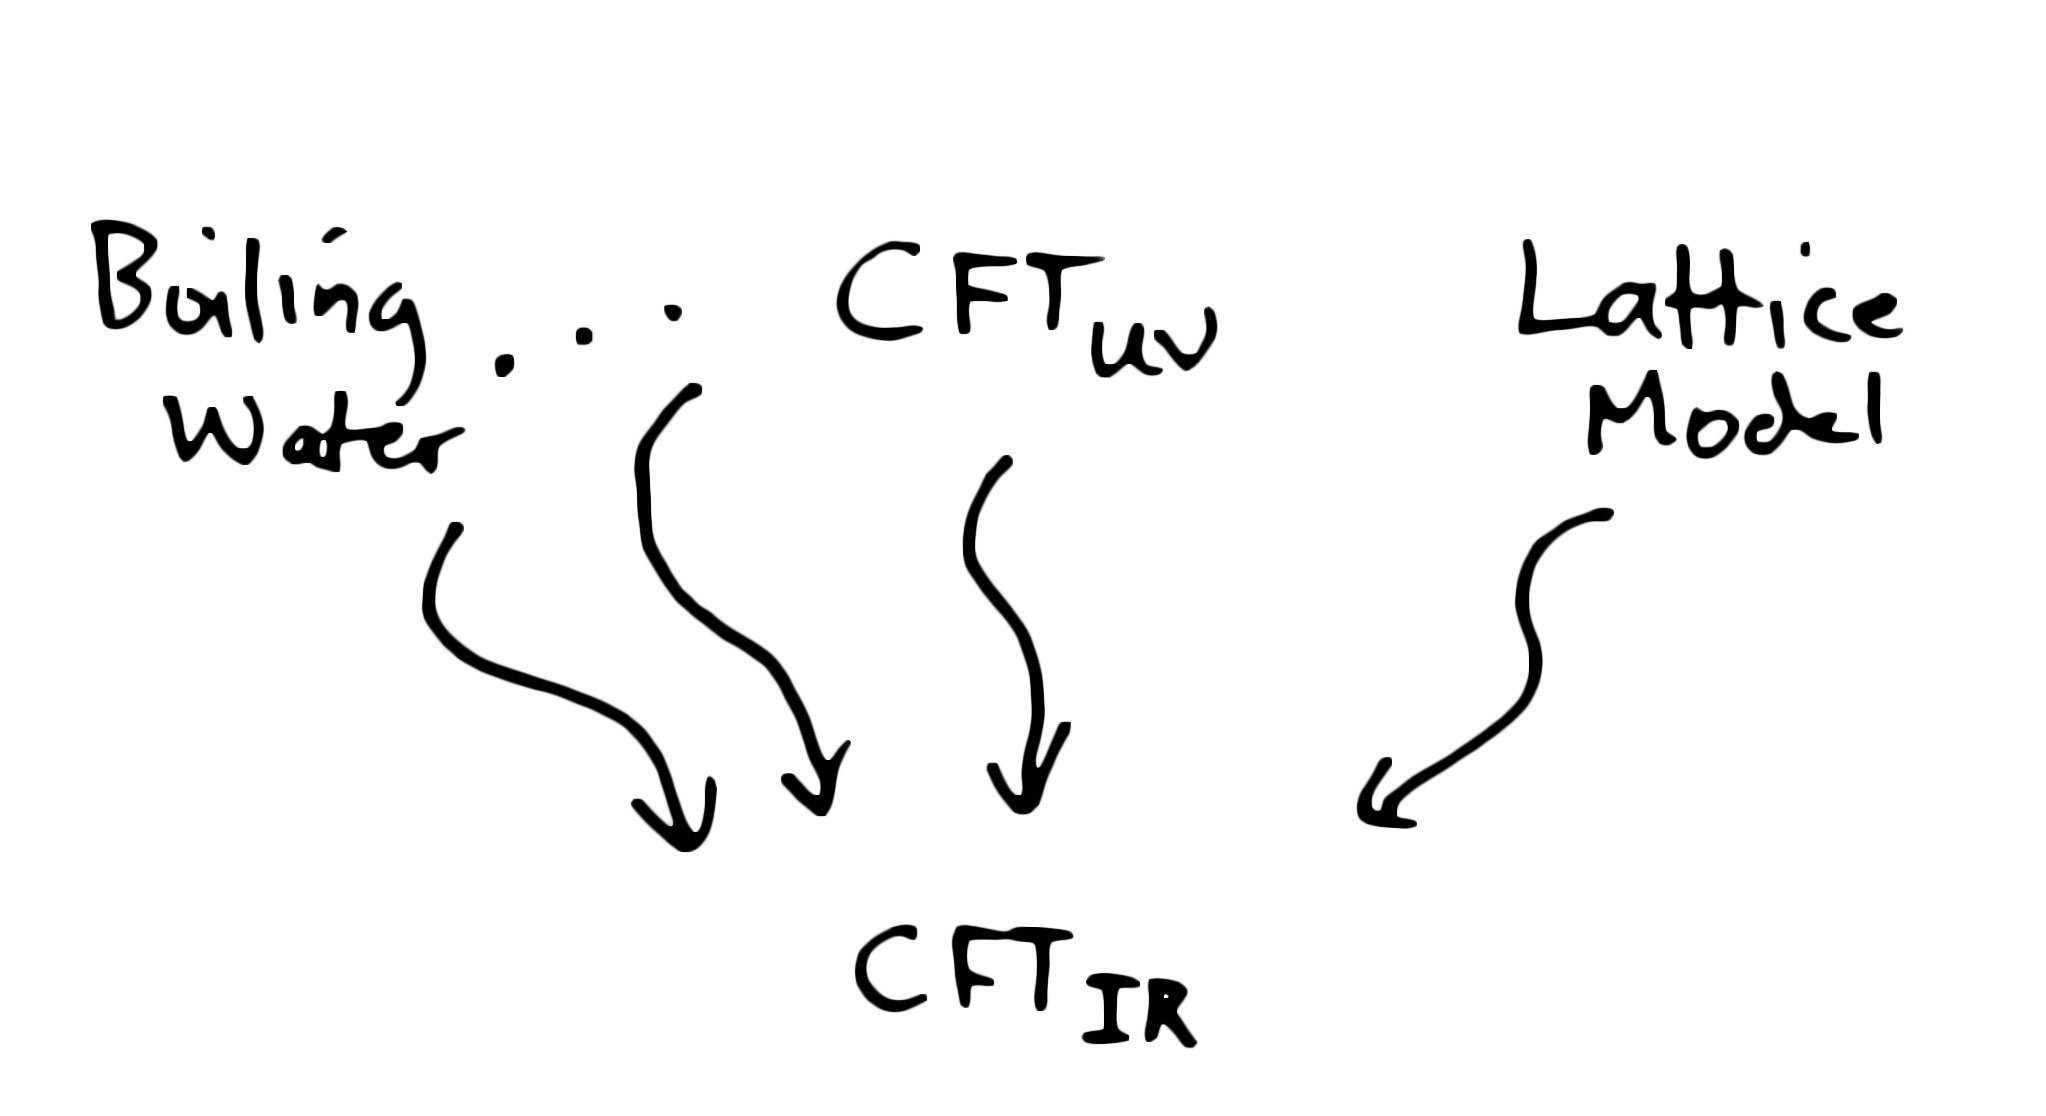
\includegraphics[width=0.55\textwidth]{rgflows-ising.jpg}
\end{center}
\caption{Many  microscopic theories can flow to the same IR CFT\@. We say that the theories are IR equivalent, or IR dual. \label{fig:rgflows}}
\end{figure}

The theory with action (\ref{eq:continuumphifour}) and $m^2/g^2=r_c$ is equivalent to the free boson at short distances (high energies/UV) and the Ising CFT at long distances (low energies/IR). The free boson is itself a CFT, so we have an RG flow from one CFT to another (figure \ref{fig:rgflows}). This construction, where we start with a UV CFT and  perturb it so that it flows to an IR CFT, is one possible definition of a general QFT. In this definition, we must allow for the possibility that the IR theory is gapped, in which case $\mathrm{CFT}_\mathrm{IR}$ is a TQFT which is technically a special case of a CFT (where all local correlation functions are zero).

An RG flow from the free boson is perhaps the cleanest theoretical construction of the Ising CFT. It shows that the Ising CFT inherits properties of a continuum quantum field theory. For example, $\f^4$-theory has rotational invariance and $\Z_2$ symmetry, so the Ising CFT does too. The Ising lattice model is easier to simulate, but it does not have microscopic rotational symmetry. Meanwhile, water has rotational symmetry but no microscopic $\Z_2$ symmetry. We will learn a lot about the Ising CFT by going back and forth between different microscopic realizations.

\subsubsection{Other universality classes}

We have seen several different systems that fall into the Ising universality class. However, not every critical point is described by the Ising CFT. Another important class of 3d CFTs are the $O(N)$ models. These can be described as the critical point of a theory of $N$ bosons $\f_i$ ($i=1,\dots,N$) with a quartic interaction that respects an $O(N)$ global symmetry
\be
S &= \int d^3 x \p{\frac 1 2 \sum_i \ptl_\mu \f_i \ptl^\mu \f_i + \frac 1 2 m^2 \sum_i \f_i \f_i + g \p{\sum_i \f_i \f_i}^2}.
\ee
XY magnets are in the same universality class of the $O(2)$ model and Heisenberg magnets are in the same universality class of the $O(3)$ model.

\draftnote{Discuss non-uniqueness of UV Lagrangian description. An example is particle-vortex duality between the gauged $O(2)$ model and the $O(2)$ model. Distinguish between IR duality and exact duality.}

But this is just the tip of the iceberg --- there is a huge zoo of different types of critical points that we can construct in a variety of ways. One of our goals will be to better understand this zoo.

\section[Path integrals, quantization, and the quantum-classical correspondence]{Path integrals, quantization, and the quantum-classical correspondence\footnote{Sources for this section: McGreevy \cite{McGreevy2017}.}}

In this section, we explain in more detail why classical statistical systems are described by Euclidean quantum field theory, and also how they are related to quantum condensed-matter systems via Wick rotation. Along the way, we will introduce some important technical concepts in QFT, like cutting-and-gluing rules for path integrals and the idea of quantization.

\subsection{The 1d Ising model and the transfer matrix}

Let us start with the Ising lattice model in 1-dimension. For concreteness, we will study the theory on a periodic lattice with length $M$, so the spins $s_i$ are labeled by $i\in \Z_M$.  The partition function is given by
\be
Z_1 &= \sum_{\{s_i=\pm 1\}} e^{-S[s]} \nn\\
S[s] &= -K \sum_{i=1}^{M} s_i s_{i+1} - h \sum_{i=1}^M s_i.
\ee
We refer to $S[s]$ as the ``action," even though it is equal to $\b H$, where $H$ is the classical Hamiltonian. This is because we would like to reserve the word Hamiltonian for a completely different object that will appear shortly.

As mentioned in the introduction, the partition sum should be thought of as a discrete version of a 1-dimensional path-integral. This 1-dimensional path integral can be computed by relating it to a 0-dimensional quantum theory. This is an example of the notion of {\it quantization}.

The key idea is to build up the partition sum by moving along the lattice site-by-site. Forget about periodicity for the moment, and consider the contribution to the partition function from spins $j<i$ for some fixed $i$,
\be
Z_\mathrm{partial}(i,s_i) &= \sum_{\{s_j:j<i\}} e^{K\sum_{j < i} s_j s_{j+1} + h \sum_{j< i} s_j}.
\ee
Because of the interaction term $s_{i-1}s_{i}$, we cannot do the sum over $\{s_1,\dots, s_{i-1}\}$ without specifying the spin $s_i$. Thus, we have a function of $s_i$. In short, $Z_\mathrm{partial}(i,s)$ is the partition function of the theory on the lattice $1\dots i$, with fixed boundary condition $s$ at site $i$.\footnote{We must also impose some boundary condition at site $1$. The precise choice is not important for this discussion, so we have left it implicit.}

Note that $Z_\mathrm{partial}(i+1,s_{i+1})$ can be related to $Z_\mathrm{partial}(i,s_{i})$ by inserting the remaining Boltzmann weights that depend on $s_i$ and performing the sum over $s_i=\pm 1$,
\be
\label{eq:onestepsum}
Z_\mathrm{partial}(i+1,s_{i+1}) &= \sum_{s_i = \pm 1} T(s_{i+1},s_i) Z_\mathrm{partial}(i,s_{i}),
\ee
where
\be
T(s_{i+1},s_i) &\equiv e^{K s_i s_{i+1} + h s_i}.
\ee

The key step is to recognize (\ref{eq:onestepsum}) as a discrete version of the Schrodinger equation in a 2-dimensional Hilbert space $\mathcal{H}$. This Hilbert space has basis $|s\>=|\pm 1\>$. The $T(s',s)$'s are elements of a $2\x 2$  matrix $\hat{T}$ acting  on $\mathcal{H}$
%We can think of $T(s',s)$ as elements of a $2\x 2$ matrix and $Z_\mathrm{partial}(s)$ as components of a vector in a 2-dimensional Hilbert space,
\be
T(s',s) &= \<s'|\hat{T}|s\>,\qquad \hat{T} =
\begin{pmatrix}
e^{K+h} & e^{-K-h} \\
e^{-K+h} & e^{K-h}
\end{pmatrix},
\ee
and $Z_\mathrm{partial}(i,s)$ are the components of a vector $|\Psi_i\>\in \mathcal{H}$,
\be
Z_\mathrm{partial}(i,s) &= \<s|\Psi_i\>.
\ee
In this notation, (\ref{eq:onestepsum}) becomes
\be
\label{eq:discreteshrodinger}
|\Psi_{i+1}\> &= \hat{T} |\Psi_i\>.
\ee
The matrix $\hat{T}$ is called the ``transfer matrix", and it plays the role of a discrete time-translation operator. Here, $i$ should be thought of as a discrete Euclidean time coordinate.

To be explicit, the (integrated) Schrodinger equation in a quantum theory in Euclidean time is
\be
|\Psi(\tau+\Delta\tau)\> &= e^{-\De\tau \hat H} |\Psi(\tau)\>,
\ee
where $\tau$ is the Euclidean time coordinate, $\De\tau$ is some time-step, and $\hat H$ is the quantum Hamiltonian. Thus,  the $1$-dimensional Ising lattice model is equivalent to a 2-state quantum theory with Hamiltonian
\be
\hat H &= -\frac{1}{\Delta\tau} \log \hat T.
\ee

When the lattice is periodic, the partition function is related to the transfer matrix by
\be
\label{eq:partitionfunctionastransfermatrix}
Z_1 %&= \sum_{\{s_i\}} T(s_M, s_{M-1}) T(s_{M-1},s_{M-2}) \cdots T(s_1,s_M) \nn\\
&= \sum_{\{s_i\}} \<s_M|\hat{T}|s_{M-1}\>\<s_{M-1}|\hat{T}|s_{M-2}\> \cdots \< s_1|\hat{T}|s_M\> \nn\\
&= \Tr(\hat{T}^M).
\ee
This is now easy to evaluate by diagonalizing $\hat T$,
\be
\Tr(\hat{T}^M) &= \l_+^M + \l_-^M,
\ee
where
\be
\l_\pm &= e^K \cosh h \pm \sqrt{e^{2K} \sinh^2 h + e^{-2K}} \nn\\
&\to \begin{cases}
2\cosh K \\
2\sinh K
\end{cases}\qquad (\textrm{when }h=0).
\ee

In the thermodynamic limit $M\to\oo$, the partition function is dominated by the larger eigenvalue
\be
Z_1 &=\l_+^M \p{1+\p{\frac{\l_-}{\l_+}}^M} \approx \l_+^M.
\ee
In quantum mechanical language, the state with the largest eigenvalue of $\hat T$ has the smallest eigenvalue of $\hat H$ --- i.e.\ it is the ground state, and we should call it $|0\>$. We have shown that the ground state dominates the thermodynamic limit. Contributions from the excited state are exponentially suppressed in the energy gap times the size of the system
\be
\p{\frac{\l_-}{\l_+}}^M &= e^{-(M\Delta\tau) m_\mathrm{gap}}, \nn\\
m_\mathrm{gap} &\equiv - \frac 1 {\Delta \tau} \log (\l_-/\l_+).
\ee

\stoplecture

We can also use the transfer matrix to compute correlation functions. For example, consider the two-point function $\<s_{i_1} s_{i_2}\>_{\Z_M}$ where the subscript $M$ indicates that we are on a periodic lattice with length $M$. Suppose $i_1>i_2$. We have
\be
\<s_{i_1} s_{i_2} \>_{\Z_M} &= \frac 1 {Z_1} \sum_{\{s_i\}} \<s_M|\hat{T}|s_{M-1}\> \cdots \<s_{i_1+1}|\hat{T}|s_{i_1}\> s_{i_1} \<s_{i_1}|\hat{T}|s_{i_1-1}\>\cdots \nn\\
& \qquad \x\cdots\<s_{i_2+1}|\hat{T}|s_{i_2}\> s_{i_2} \<s_{i_2}|\hat{T}|s_{i_2-1}\>\cdots \<s_1|\hat{T}|s_M\> \nn\\
&= \frac{1}{Z_1}\Tr(\hat{T}^{M-i_1} \hat{\s}^z \hat{T}^{i_1 - i_2}\s^z \hat T^{i_2}) \qquad (i_1 > i_2).
\label{eq:correlatorastrace}
\ee
Here, we introduced the Pauli spin operator $\s^z$ that measures the spin of a state
\be
\s^z|s\> &= s|s\>.
\ee
It is easy to compute the correlation function (\ref{eq:correlatorastrace}) by expressing $\hat s$ in the eigenbasis of $\hat T$.
\begin{exercise}
Show that in the limit of large $M$ and large ``distance" $i_1-i_2$, the correlator factorizes into a product of expectation values $\<0|\s^z|0\>$, plus exponential corrections from the excited state
\be
\<s_{i_1} s_{i_2}\>_{\Z_M} &= \<0|\s^z|0\>^2 + O(e^{-m_\mathrm{gap} \tau}, e^{- m_\mathrm{gap}(L-\tau)}),
\ee
where $\tau\equiv (i_1-i_2)\Delta\tau$, $L\equiv M\Delta\tau$.
\end{exercise}

Let us write (\ref{eq:correlatorastrace}) in a slightly different way by introducing ``Heisenberg picture" operators
\be
\hat s(i) &= \hat T^{-i} \s^z \hat T^i.
\ee
Equation~(\ref{eq:correlatorastrace}) is equivalent to
\be
\label{eq:heisenbergtwopt}
\<s_{i_1} s_{i_2}\>_{\Z_M} &= \frac 1 {Z_1} \Tr(\hat s(i_1) \hat s(i_2) \hat T^M) \qquad (i_1 > i_2).
\ee
Note that in deriving (\ref{eq:correlatorastrace}, \ref{eq:heisenbergtwopt}), we used that $i_1>i_2$. If instead $i_2 > i_1$, the path integral would give a product of operators in the opposite order
\be
\<s_{i_1} s_{i_2}\>_{\Z_M} &= \frac 1 {Z_1} \Tr(\hat s(i_2) \hat s(i_1) \hat T^M ) \qquad (i_2 > i_1).
\ee
The general statement is that the path integral becomes a time-ordered product of quantum operators\footnote{We hope that the time-ordering symbol $T\{\cdots\}$ will not be confused with the transfer matrix.}
\be
\label{eq:periodiccorrelationlattice}
\<s_{i_1} \cdots s_{i_n}\>_{\Z_M} &= \frac{1}{Z_1}\Tr(T\{ \hat s(i_1) \cdots \hat s(i_n)\}\hat T^M ),
\ee
where the definition of the time-ordering symbol is
\be
T\{\hat s (i_1)\cdots \hat s(i_n)\} &\equiv \hat s(i_1)\cdots \hat s(i_n) \theta(i_1 > \cdots > i_n) + \mathrm{permutations}.
\ee
Here $\theta(i_1 > \cdots > i_n)$ is $1$ if the $i_k$ are in the specified order and zero otherwise.

Finally, in the limit of large-$M$, the factor $\frac{\hat T^M}{\l_+^M}$ projects onto the ground state, so a path integral on the full lattice $\Z$ becomes a vacuum expectation value of a time-ordered product
\be
\label{eq:fulllattice}
\<s_{i_1}\cdots s_{i_n}\>_\Z &= \<0|T\{ \hat s(i_1) \cdots \hat s(i_n)\}|0\>.
\ee

\begin{exercise}
Consider adding a next-to-nearest neighbor interaction to the 1d Ising model
\be
S[s] &= \sum_{i} K s_{i}s_{i+1} + K' s_{i} s_{i+2}.
\ee
Find the associated quantum Hilbert space and transfer matrix, and compute the partition function on $\Z_M$ in the limit of large $M$.
\end{exercise}

\subsection{Quantization in quantum mechanics}

The procedure of turning a path integral into a product of quantum operators is called quantization. It is an extremely general procedure that ultimately stems from ``cutting and gluing" rules of the path integral.

For a more familiar example, let us review quantization for the path integral of a quantum particle on the real line. This theory has Euclidean action
\be
S[x] &= \int d\tau \p{\frac 1 2 \dot x^2 + V(x)},
\ee
where $x(\tau)$ is a map from Euclidean time $\tau$ to $\R$.
%To quantize, we introduce an orthonormal basis state $|x\>$ for every classical configuration at a fixed time $\tau_0$. These are the analogs of $|s=\pm 1\>$ in the Ising case, which were in one-to-one correspondence with classical configurations at a fixed lattice site $i_0$.
Consider the path integral on the interval $\tau\in[\tau_a,\tau_b]$ with fixed boundary conditions
\be
\label{eq:qmtransitionamplitude}
U(x_b,\tau_b;x_a,\tau_a) &\equiv \int_{\substack{x(\tau_b)=x_b \\ x(\tau_a) = x_a}} Dx(\tau) e^{-S[x]}.
\ee
By grouping paths according to their positions at a fixed time $\tau_c\in(\tau_a,\tau_b)$, we obtain a simple ``gluing" rule for $U$,
\be
\label{eq:gluingruleqm}
U(x_b,\tau_b;x_a,\tau_a) &= \int_{-\oo}^\oo dx_c U(x_b,\tau_b;x_c,\tau_c)U(x_c,\tau_c;x_a,\tau_a).
\ee

To quantize the theory, we build up the path integral  in small time-increments using the gluing rule. Suppose we have already computed the path integral $U(x_0,\tau_0;x_a,\tau_a)$ on the interval $[\tau_a,\tau_0]$. To extend $\tau_0\to \tau_0+\e$, we write
\be
\label{eq:gluingforsmallinterval}
U(x_1,\tau_0+\e;x_a,\tau_a) &= \int dx_0\, U(x_1,\tau_0+\e;x_0,\tau_0) U(x_0,\tau_0;x_a,\tau_a).
\ee
The quantity
\be
U(x_1,\tau_0+\e;x_0,\tau_0) &= U(x_1,\e;x_0,0).
\ee
plays the role of a transfer matrix, and $U(x_0,\tau_0;x_a,\tau_a)$ plays the role of a state at time $\tau_0$. To see this, we introduce a Hilbert space
\be
\label{eq:qmhilberspace}
\mathcal{H} &= \mathrm{Span}\{|x\> : x\in \R\}
\ee
with inner product $\<x'|x\>=\de(x-x')$.
The $|x\>$ are analogs of the basis states $|s=\pm 1\>$ in the Ising model. Defining $\hat T_\e$ and $|\Psi(\tau_0)\>$ by
\be
\<x_1|\hat T_\e|x_0\> &= U(x_1,\e;x_0,0),\nn\\
\<x_0|\Psi(\tau_0)\> &= U(x_0,\tau_0;x_a,\tau_a),
\ee
equation (\ref{eq:gluingforsmallinterval}) becomes
\be
\label{eq:transfermatrixforqmeq}
|\Psi(\tau_0+\e)\> &= \hat T_\e |\Psi(\tau_0)\>.
\ee

To recover the Schrodinger equation, we must show that 
\be
\hat T_\e &= 1 - \e \hat H + O(\e^2),
\ee
where
\be
\hat H &= -\frac 1 2 \frac{\ptl^2}{\ptl x^2} + V(x)
\ee
is the usual quantum-mechanical Hamiltonian. This is a standard argument, and we give a quick version here for completeness. We have
\be
\<x_1|\hat T_\e|x_0\> &= \int_{\substack{x(\e)=x_1 \\ x(0) = x_0}} Dx(\tau) e^{-S[x]},\qquad(\e \ll 1)\nn\\
S[x] &= \int_0^\e d\tau \p{\frac 1 2 \dot x^2 + V(x)}.
\ee
Because the time interval is so short, if $|x(\tau)-x_0|$ ever becomes larger than $O(\e)$, the kinetic term will cause the amplitude to be highly suppressed. Thus, let us assume $|x(\tau)-x_0|$ is of order $\e$. This means we can replace $V(x)\to V(x_0)$ (up to subleading corrections in $\e$), so the potential factors out of the integrand
\be
e^{-S[x]} &= e^{-\e V(x_0)} \exp\p{-\int_0^\e d\tau \frac{\dot x^2}{2}}.
\ee

We can now split $x(\tau)$ into a classical term and a fluctuation term $\z(\tau)$ with boundary conditions $\z(0)=\z(\e)=0$,
\be
x(\tau) &= x_0\p{1-\frac{\tau}{\e}} + x_1\frac{\tau}{\e} + \z(\tau),\nn\\
\int_0^\e d\tau \frac{\dot x^2}{2} &= \frac{(x_1-x_0)}{2\e} + \int_0^\e d\tau \frac{\dot\z^2}{2}.
\ee
The path integral over $\z$ contributes a constant $A_\e$ that depends on how the theory is regulated.\footnote{A very simple regulator is to approximate $x(\tau)$ as a piecewise linear path with segments of length $\e$. This is equivalent to simply setting $\z=0$ and not doing the integral.} We thus find
\be
\<x_1|\hat T|x_0\> &= A_\e e^{-\e V(x_0)} e^{-\frac{(x_1-x_0)^2}{2\e}}(1+O(\e)).
\ee
Finally, the Gaussian factor can be expanded in $\e$ using
\be
\label{eq:simplifyexponential}
e^{-\frac{x^2}{2\e}} &= \sqrt{2\pi \e}\p{\de(x) + \frac \e 2 \de''(x) + O(\e^2)},
\ee
which gives
\be
\<x_1|\hat T|x_0\> &= A_\e \sqrt{2\pi \e} \p{\de(x_1-x_0) - \e\p{-\frac 1 2\de''(x_1-x_0) + V(x_0)\de(x_1-x_0)} + O(\e^2)} \nn\\
 &= A_\e \sqrt{2\pi \e}\<x_1|1 - \e \hat H + O(\e^2)|x_0\>.
\ee
The prefactor $A_\e \sqrt{2\pi \e}$ is an overall regulator-dependent constant that can be renormalized away by adding a ``cosmological constant" term to the action.

Thus, in the limit $\e\to 0$, equation (\ref{eq:transfermatrixforqmeq}) becomes a Euclidean version of the Schrodinger equation
\be
\frac{d}{d\tau} |\Psi(\tau)\> &= - \hat H|\Psi(\tau)\>.
\ee
Integrating using the initial condition $U(x',0,x,0)=\de(x-x')$, we find
\be
\label{eq:pathintegralwithbcsasamplitude}
U(x_b,\tau_b;x_a,\tau_a) &= \<x_b|e^{-\hat H (\tau_b-\tau_a)} |x_b\>.
\ee

Path integrals on different geometries correspond to different quantum mechanical observables. For example, the path integral on a circle $S^1_\b$ of length $\b$ with periodic boundary conditions is equal to
\be
\int_{-\oo}^\oo dx\, U(x,\b;x,0) = \Tr(e^{-\b \hat H}),
\ee
which is the quantum partition function at inverse temperature $\b$.
This is the continuum analog of equation~(\ref{eq:partitionfunctionastransfermatrix}).
Inserting observables into the path integral gives a time-ordered product of the associated quantum operators. For example, with periodic boundary conditions,
\be
\label{eq:periodiccorrelation}
\<x(\tau_1) \cdots x(\tau_n)\>_{S^1_\b} &=
\int_{x(\b)=x(0)} Dx\, x(\tau_1) \cdots x(\tau_n) e^{-S[x]}\nn\\
 &= \Tr(T\{\hat x(\tau_1) \cdots \hat x(\tau_n)\} e^{-\b \hat H}),
\ee
where we introduced the operator
\be
\hat x(\tau) &= e^{\tau \hat H} \hat x e^{-\tau \hat H}, \nn\\
\hat x|x\> &= x|x\>.
\ee
To derive (\ref{eq:periodiccorrelation}), we cut the interval $[0,\b]$ into segments $[0,\tau_1]\cup [\tau_1,\tau_2] \cup \cdots [\tau_n,\b]$ (assuming $\tau_n > \cdots > \tau_1$) and use (\ref{eq:pathintegralwithbcsasamplitude}) for each segment.
The operator $\hat x$ is the analog of $\hat s$ and equation~(\ref{eq:periodiccorrelation}) is the analog of (\ref{eq:periodiccorrelationlattice}).

Finally, in the limit $\b\to \oo$, the factor $e^{-\b \hat H}$ projects onto the ground state. Thus the Euclidean path integral on $\R$ is equal to a time-ordered correlation function in the ground state,
\be
\<x(\tau_1) \cdots x(\tau_n)\>_{\R} &= \<0|T\{\hat x(\tau_1) \cdots \hat x(\tau_n)\}|0\>.
\ee
This is the continuum analog of (\ref{eq:fulllattice}).

\stoplecture

\subsection{The 2d Ising model}

Let us now consider a slightly more complicated case: the 2d Ising model. This will be a good toy example for how cutting, gluing, and quantization work in a general QFT. For simplicity, we set $h=0$. We consider the partition function on the doubly-periodic lattice $\Z_{M} \x \Z_{N}$ and label spins $s_{i,j}$ by a pair $(i,j) \in \Z_{M} \x \Z_{N}$.

The action is given by
\be
S[s] &= -K\sum_{i,j} (s_{i,j}s_{i+1,j}  +  s_{i,j}s_{i,j+1}) \nn\\
&= K \sum_{i,j} \p{\frac 1 2 (s_{i,j+1} - s_{i,j})^2 - 1} - K \sum_{i,j}  s_{i,j} s_{i+1,j} \nn\\
&= \mathrm{const.} + \sum_{j=1}^{N} L( \bs_{j+1}, \bs_{j}).
\label{eq:unimportant}
\ee
In the last line, we split the action into contributions from pairs of neighboring rows.
The notation $s_{j}$ represents the configuration of spins in the $j$-th row,
\be
(\bs_{j})_{i} &= s_{i,j}.
\ee
The action associated with a pair of neighboring rows is given by
\be
L(\bs',\bs) &= \frac 1 2 K \sum_{i=1}^{M}(\bs'_i - \bs_i)^2 - \frac 1 2 K \sum_{i=1}^{M}(\bs_{i+1} \bs_i + \bs'_{i+1} \bs'_i).
\ee
(The constant in (\ref{eq:unimportant}) gives an unimportant multiplicative constant in the path integral that will disappear in normalized correlation functions, so we will ignore it.)

To quantize the theory, we can think of the $j$ direction as time, so $\bs_{j}$ is interpreted as a classical configuration on a fixed time-slice. The Hilbert space has an orthonormal basis vector for each such configuration,
\be
\label{eq:twodisinghilbert}
\mathcal{H}_{M} &= \mathrm{Span}\left\{|\pm\! 1, \pm 1, \cdots,\pm 1\>\right\} \nn\\
&= \bigotimes_{i=1}^{M} \mathcal{H}_i,
\ee
where $\mathcal{H}_i$ is a 1-qubit Hilbert space for each site $i$. $\mathcal{H}_{M}$ is the quantum Hilbert space of $M$ qubits, and is $2^{M}$-dimensional.

The transfer matrix between successive time slices is a $2^{M} \x 2^{M}$ matrix with entries
\be
\<\bs'|\hat T|\bs\> &= e^{-L(\bs',\bs)}.
\ee
The partition function on $\Z_{M} \x \Z_{N}$ is then
\be
\label{eq:partitionfunctionastracetwod}
Z(\Z_{M} \x \Z_{N}) &= \Tr_{\mathcal{H}_{M}}(\hat T^{N}).
\ee
To compute correlation functions, we need an operator that measures the spin at site $i$. This is simply the Pauli spin matrix $\s^z_i$ associated with the $i$-th site
\be
\s^z_i |s_1,\dots,s_j,\dots,s_{M}\> &= s_i |s_1,\dots,s_i,\dots,s_{M}\>.
\ee
We also have Heisenberg picture operators
\be
\label{eq:oldspinop}
\hat s_{i,j} &= \hat T^{-j} \s_i^z \hat T^j.
\ee
Correlation functions become traces of time-ordered products, e.g.
\be
\<s_{i_1,j_1} s_{i_2,j_2}\> &= \Tr_{\mathcal{H}_{M}}(\hat T^{N+j_2-j_1} \s_{i_1}^z \hat T_2^{j_1-j_2} \s_{i_2}^z) \th (j_1-j_2) + (1\leftrightarrow 2) \nn\\
&= \Tr_{\mathcal{H}_M}(T\{\hat s_{i_1,j_1} \hat s_{i_2,j_2}\} \hat T^{N}).
\ee

Let us now emphasize an important new ingredient in the 2-dimensional case compared to the 1-dimensional case. To arrive at (\ref{eq:partitionfunctionastracetwod}), we had to choose $j$ as the time direction. We then cut the path integral along rows of constant $j$. However, we could just as well have chosen $i$ as the time direction and cut the path integral along columns of constant $i$. This would give a different Hilbert space $\mathcal{H}_N$ with dimension $2^N$, a new transfer matrix $\hat T'$ (acting on $\mathcal{H}_N$), and a different formula for the same path integral,
\be
Z(\Z_M\x\Z_N) &= \Tr_{\mathcal{H}_N}(\hat T'^M) = \Tr_{\mathcal{H}_M}(\hat T^N).
\ee
In this new quantization, an insertion of $s_{i,j}$ in the path integral becomes an insertion of
\be
\label{eq:newspinop}
s_{i,j} &\to \hat T'^{-i} \s_j^z \hat T'^i
\ee
in a time-ordered product of quantum operators. Let us emphasize that the operators (\ref{eq:oldspinop}) and (\ref{eq:newspinop}) truly are different, even though they represent the same path integral variable. They even act on different-dimensional Hilbert spaces ($2^M$ vs.\ $2^N$)! Furthermore, even the notion of ``time"-ordering is different in this different quantization: in one case, operators are ordered according to their $i$ coordinates, and in the other they are ordered according to their $j$ coordinates.

\begin{exercise}
Show how to quantize the 2d Ising model in yet another way, using $i+j$ as the time coordinate and $i-j$ as space coordinate. What is the Hilbert space? What is the transfer matrix?
\end{exercise}

%More generally, we can build up the 2d Ising path integral by cutting and gluing path integrals on arbitrary regions on the lattice. For example, given a subset of spins $B\subset \Z^2$, let the ``boundary" $\ptl B$ consist of the spins in $B$ that have nontrivial interactions with spins outside of $B$. We use $s_b$ to indicate spins in the boundary $\ptl B$ and $s_i$ to indicate spins in the interior. We can associate a Hilbert space to $\ptl B$ by introducing an orthonormal basis vector for every spin configuration on $\ptl B$,
%\be
%\mathcal{H}_{\ptl B} &= \mathrm{Span}\left\{|s_b\> : \textrm{$s_b$ is a configuration of spins on $\ptl B$} \right\}.
%\ee
%The path integral over the interior with fixed boundary conditions gives a state $|\Psi\> \in \mathcal{H}$ with wavefunction
%\be
%\<s_{b 0}|\Psi\> &= \sum_{\substack {s_i=\pm 1 \\ s_b = s_{b0}}} e^{-S[s]}.
%\ee
%Consider now the complement $\bar B$, which also has $\ptl B$ as a boundary, and let $|\Psi'\>\in \mathcal{H}$ be the state produced by performing the path integral over the interior of $\bar B$. The path integral over $\bar B\cup B$ is given by taking a product of the associated wavefunctions and summing over boundary spins 
%\be
%Z(\bar B\cup B) &= \sum_{s_b} \<\Psi'|s_b\>\<s_{b}|\Psi\> = \<\Psi'|\Psi\>.
%\ee
%
%In general when two regions $B_1,B_2$ share part of their boundary, we can partially glue states in $\mathcal{H}_{\ptl B_1}$ and $\mathcal{H}_{\ptl B_2}$ by summing over the shared boundary spins. This gives a state in the Hilbert space $\mathcal{H}_{\ptl(B_1\cup B_2)}$ (figure~\ref{}).
%
%In the special case where we cut the path integral into pieces related by a translation symmetry, we can introduce a transfer matrix and interpret correlators in terms of time-ordered products of quantum operators.

\subsection{Atiyah-Segal axioms}
\label{sec:asaxioms}

We are now ready to understand some axioms of continuum QFT. We will simultaneously state them and give examples in a Lagrangian theory of a real scalar field $\f$. A version of these axioms in TQFTs is due to Atiyah and a version in 2d CFTs is due to Segal. We will be interested in QFTs that depend on the geometry of the space in which they live, so when we say ``manifold" below, we mean ``Riemannian manifold with metric."

Consider a $d$-dimensional QFT $Q$. 
\begin{enumerate}
\item To every $(d-1)$-manifold $N$ without boundary, $Q$ assigns a Hilbert space $\mathcal{H}_{N}$ called the space of states on $N$.

For example, in theories with an explicit path integral over some fields (``Lagrangian theories"), $\mathcal{H}_N$ has an orthonormal basis state for every field configuration on $N$. In scalar field theory,
\be
\label{eq:scalarfieldhilbertspace}
\mathcal{H}_N &= \mathrm{Span}\{|\f_b\> : \f_b\in C(N,\R)\}.
\ee
with inner product $\<\f_{b1}|\f_{b2}\> = \de(\f_{b1}-\f_{b2})$ (a functional $\de$-function).

Here $C(N,\R)$ is a space of real-valued functions on $N$.\footnote{We are being deliberately vague about {\it which\/} space of functions on $N$, e.g.\ $C^1(N)$, $C^\oo(N)$, etc.. In reality, the path integral is defined by introducing a regulator and taking a limit as the regulator is removed. Different regulators will result in different spaces of functions, and we prefer to be agnostic about which regulator is being used.}  More formally, we can write
\be
\cH_N &= L^2(C(N,\R),\C),
\ee
where $L^2(X)$ denotes the square-integrable complex functions on $X$.

The space $\cH_N$ is the analog of the Hilbert spaces (\ref{eq:qmhilberspace}) and (\ref{eq:twodisinghilbert}) for quantum mechanics and the 2d Ising model. Let us discuss the example of quantum mechanics more explicitly. Quantum mechanics is a $1$-dimensional QFT. In this case $d-1=0$, and the only possible $0$-manifolds are disjoint unions of points. The space of field configurations on a point is $C(\bullet,\R)=\R$, so the Hilbert space associated to a point is $\cH_\bullet = L^2(C(\bullet,\R),\C) = L^2(\R,\C)$. This is spanned by the usual basis states $|x\>$ with inner product $\de(x-x')$.\footnote{Note in particular that $L^2(C(\bullet,\R),\C)$ is totally different from $L^2(\bullet,\C)=\C$. In general, don't confuse the Hilbert space $\cH_N$ with the space of square-integrable functions $L^2(N,\C)$.}

%Note that $L^2(C(N,\R),\C)$ totally different from $L^2(N,\C)$. To understand this, consider the special case of quantum mechanics, which is a $1$-dimensional QFT. The only possible $(d-1)$-manifolds are then disjoint unions of points. The space of fields on a point is $C(\bullet,\R)=\R$, so the Hilbert space is $\cH_\bullet = L^2(C(\bullet,\R)) = L^2(\R,\C)$. This is spanned by the usual basis states $|x\>$ with inner product $\de(x-x')$. This is not the same as $L^2(\bullet,\C)=\C$.

\item The space of states on a disconnected union is a tensor product
\be
\label{eq:disjointunionrule}
\mathcal{H}_{N_1 \sqcup N_2} &= \mathcal{H}_{N_1}\otimes \mathcal{H}_{N_2}.
\ee
This should be clear in scalar theory from the definition (\ref{eq:scalarfieldhilbertspace}). It will be useful to assign a Hilbert space to the empty manifold, and the only reasonable choice consistent with (\ref{eq:disjointunionrule}) is
\be
\mathcal{H}_{\varnothing} &= \mathbb{C}.
\ee

\item To every $d$-manifold $M$ with incoming boundary $N$ and outgoing boundary $N'$, $Q$ assigns a transition amplitude\footnote{By incoming vs. outgoing boundary, we assume that each boundary component $N$ comes equipped with a nonzero infinitesimal vector field pointing into or out of $M$.}
\be
\label{eq:transitionamplitude}
Z_M : \mathcal{H}_N \to \mathcal{H}_{N'}.
\ee
In Lagrangian theories, $Z_M$ is obtained by fixing boundary conditions on $N,N'$ and performing the path integral over the interior. For example in a scalar theory, the matrix elements of $Z_M$ are given by
\be
\label{eq:transitionmatrixelement}
\<\f_b'|Z_M|\f_{b}\> &= \int_{\substack{\phi|_{N} = \f_b \\ \phi|_{N'} = \f_b'}} D\phi(x) e^{-S[\f]}.
\ee
Here, the notation $\f|_{N}$ means the restriction of $\f$ to $N$.

In the special case where $M$ is a closed manifold (without boundary), $Z_M$ is a linear map
\be
\label{eq:closedmanifold}
Z_M : \mathbb{C} \to \mathbb{C}.
\ee
A linear map $\C\to\C$ is simply multiplication by complex number. That number is the ``partition function" of the QFT on $M$.

Another important case is where $M$ has boundaries $(\varnothing,N)$. (The first element of the ordered pair is the incoming boundary and the second is the outgoing boundary.) In this case, $Z_M$ gives a linear map
\be
\label{eq:outgoingboundary}
Z_M: \C \to \mathcal{H}_N.
\ee
Any such map is uniquely determined by its action on $1\in \C$, so this is equivalent to a state $|\Psi\>=Z_M(1) \in \mathcal{H}_N$. Thus, we can ``prepare a state" by performing the path integral with fixed boundary conditions. We saw several examples in the previous sections, for example the definition of $Z_\mathrm{partial}(i,s)$ in the 1d Ising model.

Finally, consider the case where $M$ has boundaries $(N,\varnothing)$. Then we have a linear map
\be
\label{eq:incomingboundary}
Z_M: \mathcal{H}_N \to \C,
\ee
which is equivalent to a bra-state $\<\Psi|\in \mathcal{H}_N^*$.

The usefulness of assigning $\mathcal{H}_\varnothing=\C$ is that all these special cases (\ref{eq:closedmanifold}, \ref{eq:outgoingboundary}, \ref{eq:incomingboundary}) are covered by one axiom (\ref{eq:transitionamplitude}).

\item Suppose $M_1$ has boundaries $(N,N')$ and $M_2$ has boundaries $(N',N'')$.  We can form a new $d$-manifold $M_1\cup_{N'} M_2$ by gluing $M_1$ and $M_2$ along $N'$. This manifold has boundaries $(N,N'')$. The total transition amplitude is the composition
\be
\label{eq:compositionrule}
Z_{M_1\cup_{N'} M_2} &= Z_{M_2} Z_{M_1} : \mathcal{H}_N \to \mathcal{H}_{N''}.
\ee

In scalar field theory, this follows by cutting the path integral along $N'$ by fixing boundary conditions $\f_b'\in C(N',\R)$, and then finally performing the $(d-1)$-dimensional path integral over $\f_b'$,
\be
&\int_{\substack{\phi|_{N} = \f_b \\ \phi|_{N''} = \f_b''}} D\phi(x) e^{-S[\f]} \nn\\
&= \int_{y\in N'} D\f_b'(y)
\int_{\substack{\phi_2|_{N'} = \f_b' \\ \phi_1|_{N''} = \f_b'' \\ x \in M_2}} D\phi_2(x) e^{-S[\f_2]}
\int_{\substack{\phi_1|_{N} = \f_b \\ \phi_1|_{N'} = \f_b' \\ x \in M_1}} D\phi_1(x) e^{-S[\f_1]}.
\ee
This is the field-theory analog of our gluing rule for transition amplitudes in quantum mechanics (\ref{eq:gluingruleqm}).
In the notation (\ref{eq:transitionmatrixelement}), we have simply inserted a complete set of states on $N'$,
\be
\<\f_b''|Z_{M_2} Z_{M_1}|\f_b\> &= \int_{y\in N'} D\f'_b(y) \<\f_b''|Z_{M_2}|\f_b'\>\<\f_b'|Z_{M_1}|\f_b\>.
\ee

\item \draftnote{Describe generalization to correlation functions.}

\item \draftnote{Discuss orientation, orientation reversal, conjugation.}

\end{enumerate}

\draftnote{Discuss the possibility of giving the manifolds different amounts of structure, for instance topological structure, a Riemannian metric, etc. In these notes, we will initially be interested in manifolds with a metric. Later, we will see that in certain cases we can relax this structure to only a conformal class of metrics.}

Although we have given explicit prescriptions in the case of a continuum theory, all of these axioms have analogs in the case of the 2d Ising model. It is not hard to imagine how the continuum axioms might arise in the continuum limit of the Ising model, at least in the case where the ``manifolds" $M,N,\dots$ are regions of flat space.

\stoplecture

\subsection{Quantization in continuum QFT}

Let us use the above axioms to describe the quantization procedure one more time, now in continuum QFT.
Consider the $d$-manifold $M_L=I_{L} \x N$, where $I_L=[0,L]$ is an interval of length $L$ and $N$ is a $(d-1)$-manifold, and suppose $M_L$ is endowed with the product metric. The composition rule (\ref{eq:compositionrule}) implies that
\be
\label{eq:exponentiatedtransition}
Z_{M_L} &= e^{-L \hat H}
\ee
for some operator
\be
\hat H:\mathcal{H}_N \to \mathcal{H}_N,
\ee
namely the Hamiltonian.

Consider a correlation function on $S_\b^1 \x N$
\be
\label{eq:correlatorcontinuum}
\<\f(\tau_1,y_1)\cdots \f(\tau_n,y_n)\>_{S_\b^1 \x N} &= 
\int_{\f(\b,y)=\f(0,y)} D\f(x)\, \f(\tau_1,y_1)\cdots \f(\tau_n,y_n) e^{-S[\f]}.
\ee
Here, $\tau,y$ are coordinates on $S_\b^1,N$, respectively.
As before, we introduce operators $\hat \f(y)$ that measure the field configuration on a time-slice
\be
\hat \f(y)|\f_b\> &= \f_b(y)|\f_b\>.
\ee
To compute (\ref{eq:correlatorcontinuum}), we cut the path integral at times $\tau_1,\dots,\tau_n$ and repeatedly use (\ref{eq:exponentiatedtransition}). By the usual logic, this gives
\be
\<\f(\tau_1,y_1)\cdots \f(\tau_n,y_n)\>_{S_\b^1 \x N} &= \Tr_{\mathcal{H}_N}(e^{-\b\hat H} T\{\hat \f(\tau_1,y_1)\cdots \hat \f(\tau_n,y_n)\}),
\ee
where
\be
\hat \f(\tau,y) &\equiv e^{\tau \hat H} \hat \f(y) e^{-\tau \hat H},
\ee
and $T\{\cdots\}$ represents time ordering in $\tau$.
Taking the limit of a long interval, the factor $e^{-\b \hat H}$ projects onto the ground state, and we obtain\footnote{In (\ref{eq:limitoflongbeta}), we are assuming that the theory has a unique ground state on $N$. More generally, there might be multiple ground states on $N$, in which case the limit $\b\to \oo$ becomes a trace in the space of ground states.}
\be
\label{eq:limitoflongbeta}
\<\f(\tau_1,y_1)\cdots \f(\tau_n,y_n)\>_{\R \x N} &=\<0|T\{\hat \f(\tau_1,y_1)\cdots \hat \f(\tau_n,y_n)\}|0\>.
\ee

For a QFT in $\R^d$, we can quantize the theory in many different ways by choosing different directions to play the role of ``time." In every quantization of the theory, we have
\be
\<\f(x_1)\cdots \f(x_n)\>_{\R^d} &= \<0|T\{\hat \f(x_1)\cdots \hat \f(x_n)\}|0\>.
\ee
However, in different quantizations, the objects appearing on the right-hand side are different. The Hilbert spaces are different (though isomorphic if the theory is $\SO(d)$-invariant), the ground states $|0\>$ are different, the quantum operators $\hat\f(x)$ are different, and the time-ordering symbols means different things. However, because they originate from a single path integral, the resulting expectation values are the same. It is sometimes useful to think of expressions like the RHS above as ``interpretations" of one underlying path integral.

\draftnote{Discuss boundary conditions and whether we should think of $\R^d$ as having a boundary or not.}

\subsection{The quantum transverse-field Ising model}

After all this abstract nonsense, let's return to more concrete things and try to understand the critical point of the 2d Ising model. The transfer matrix $\hat T$ of the 2d Ising lattice model was diagonalized in 1944 by Onsager. Unfortunately, we won't have time to describe his solution. Instead, we will study a closely related model in the same universality class as the lattice model.

Recall that the transfer matrix has matrix elements $\<\bs'|\hat T|\bs\> = e^{-L(\bs',\bs)}$. Let us write $\hat T$ in a more familiar way as an operator on a spin chain. First split $L$ into contributions from horizontal and vertical bonds
\be
L(\bs',\bs) &= L_h(\bs')+L_h(\bs) + L_v(\bs',\bs). \nn\\
L_h(\bs) &= -\frac 1 2 K \sum_i \bs_{i+1} \bs_i, \nn\\
L_v(\bs',\bs) &= \sum_i \frac 1 2 K(\bs_i'-\bs_i)^2.
\ee
Note that
\be
e^{\frac 1 2 K \sum_i \s^z_i \s^z_{i+1}}|\bs\> &= e^{-L_h(\bs)}|\bs\>.
\ee
Meanwhile, $L_v$ only involves spins at a single site, so let us imagine that we have only one site. Note that
\be
\<s'|(1+e^{-2K}\s^x)|s\> &= e^{-\frac 1 2 K (s'-s)^2}.
\ee
We also have
\be
1+e^{-2K} \s^x &= e^{A+K' \s^x},\qquad\textrm{where} \nn\\
\tanh K' &= e^{-2K},\nn\\
e^A &= \sqrt{1-e^{-4K}},
\ee
which follows by expanding out the Taylor series for $e^{A+K'\s^x}$ and matching the coefficients of $1,\s^x$.
Thus,
\be
e^{AM}\<\bs'|e^{K' \sum_i \s^x_i}|\bs\> &= e^{-L_v(\bs',\bs)}.
\ee
The constant $e^{AM}$ will cancel in correlation functions, so we will ignore it. Putting everything together, we find
\be
\hat T &\propto \exp\p{\frac 1 2 K \sum_i \s^z_i \s^z_{i+1}} \exp\p{K' \sum_i \s^x_i} \exp\p{\frac 1 2 K \sum_i \s^z_i \s^z_{i+1}}.
\ee
In a quantum-mechanical interpretation, we would write $\hat T=e^{-\De\tau \hat H}$, but the resulting $\hat H$ would be very complicated.

To get the theory we'll actually study, we first allow $K',K$ to be independent parameters, and then take a limit where $K,K'$ become small with fixed ratio $K'/K=g$. These modifications may seem somewhat drastic, but it turns out that, at the critical point, they can be compensated by simply rescaling the time coordinate. (We will not prove this, unfortunately.) This results in
\be
\hat T &\to e^{-\Delta \tau \hat H},
\ee
where $\Delta\tau$ is small and the Hamiltonian $\hat H$ is relatively simple,
\be
\hat H &= \sum_i \s_i ^z \s_{i+1}^z + g \sum_i \s_i^x.
\ee
This is the Hamiltonian of the ``quantum transverse-field Ising model" (TFIM). It describes a 1-dimensional chain of quantum spins with a nearest-neighbor interaction in the $z$-direction and an applied ``transverse" magnetic field in the $x$-direction.\footnote{Don't confuse the transverse field in the quantum Ising model with the applied magnetic field $h$ in the thermodynamic Ising model. At the beginning of this discussion, we set $h=0$.}${}^{,}$\footnote{A similar procedure starting from the $d$-dimensional classical Ising model gives the quantum TFIM on a $(d-1)$-dimensional spatial lattice, which is again in the same universality class.}

\subsubsection{Solution via the Jordan-Wigner transformation}

In the remainder of this section, let us solve the TFIM by diagonalizing $\hat H$. Since our Hilbert space is a tensor product of two possible states for each site, it's tempting to think of it as a fermionic Fock space, with creation and annihilation operators
\be
\s^\pm_n &\equiv \frac 1 2 (\s^y_n \pm i \s_n^z).
\ee
This is not correct, since these operators commute rather than anticommute at different sites. However, this can be fixed with a classic trick called the Jordan-Wigner transformation. We define fermionic creation and annihilation operators
\be
c^\dag_n = \p{\prod_{i=1}^{n-1} \s^x_i} \s^+_n,\qquad c_n &= \p{\prod_{i=1}^{n-1} \s^x_i }\s_n^-,
\ee 
which now satisfy canonical anticommutation relations
\be
\label{eq:anticommut}
\{c^\dag_n,c_m\} = \de_{nm},\qquad \{c_n,c_m\}=\{c_n^\dag,c_m^\dag\} = 0.
\ee
These new creation and annihilation operators are {\it nonlocal} on the spin chain. We can think of them as creating and destroying fermionic solitons.

\begin{exercise}
Verify the anticommutation relations (\ref{eq:anticommut}).
\end{exercise}

It's perhaps not surprising that we can write nonlocal variables that behave like fermions. The surprise is that the Hamiltonian in these new variables is still local, and actually quite simple
\be
\label{eq:jordanwignerhamiltonian}
H &= \sum_{n=1}^{M-1} (c_n^\dag+c_n)(c_{n+1}^\dag-c_{n+1})-P(c_{M}^\dag+c_{M})(c_{1}^\dag-c_{1})+g\sum_{n=1}^{M}(2c_n^\dag c_n -1)
\ee
where $P = \prod_{n=1}^{M}\s_n^x=(-1)^F$ is the parity operator.  Within each parity eigenspace, the Hamiltonian becomes simply
\be
H &= \sum_{n=1}^{N} (c_n^\dag+c_n)(c_{n+1}^\dag-c_{n+1})+g\sum_{n=1}^{N}(2c_n^\dag c_n -1),
\ee
where when $P=-1$ we must impose periodic boundary conditions $c_{M+1}=c_1$, and when $P=1$ we must impose antiperiodic boundary conditions $c_{M+1}=-c_1$.\footnote{The choice of which eigenspace $P=\pm 1$ to consider is equivalent to a choice of spin structure. The TFIM is a bosonic theory and can be formulated without choosing a spin structure. However, once we introduce fermions, we are required to choose a spin structure.}  Our Hamiltonian is now translationally invariant and quadratic in creation and annihilation operators, so it can be diagonalized via a Fourier transform and Bogoliubov transformation:
\be
\label{eq:afterfourier}
H &= \sum_k \left[{-(2\cos k-2g)c_k^\dag c_k-i\sin k\p{c^\dag_{-k}c_k^\dag+c_{-k}c_k}}\right]-Mg\\
&= \sum_k \e(k)\p{b_k^\dag b_k-\frac 1 2}\label{eq:diagonalizedhamiltonian},
\ee
where $b_k^\dag$ and $b_k$ are new canonically normalized creation and annihilation operators, and
\be
\label{eq:dispersionrelation}
\e(k)&= 2\sqrt{g^2-2g\cos(k)+1}
\ee
is the dispersion relation for the free fermionic quasiparticles created by $b^\dag_k$.  Because of the boundary conditions imposed by parity, the quasimomenta must take the values
\be
\label{eq:circularchainquantization}
k=
\begin{cases}
\frac{2m\pi}{M} & P=-1,\\
\frac{(2m+1)\pi}{M} & P=1.
\end{cases}
\ee
for $m=0,1,\dots,M-1$.

\draftnote{Write out the Bogoliubov transformation in more detail.}

\begin{exercise}
Derive expressions (\ref{eq:jordanwignerhamiltonian}), (\ref{eq:afterfourier}), and (\ref{eq:diagonalizedhamiltonian}).
\end{exercise}

In the continuum limit $M\to \oo$, $k$ becomes continuous. Correlation functions are dominated by the smallest values of $\e(k)$, which (assuming $g>0$) occur near $k=0$. Expanding around this point, we have
\be
\e(k)^2 &= 4(1-g)^2+ 4g k^2 + O(k^4).
\ee
Thus, the mass gap is given by $m_\mathrm{gap}=|g-1|$. At the special point $g=g_c=1$, the mass gap goes to zero and we have a critical point. Long-distance correlation functions are dominated by states with arbitrarily low energy, which requires $k\to 0$. Fur such states, we can drop the $O(k^4)$ term, and we obtain a relativistic dispersion relation\footnote{To obtain the usual dispersion relation $\e=|k|$, we need to redefine either time or space by a factor of 2.}
\be
\e(k)^2 &= 4 k^2 \qquad(g=g_c,\ k\ll 1).
\ee

To summarize, in the continuum limit, at the critical coupling, and at long distances, the quantum TFIM becomes a free relativistic fermion. This is yet another example of IR equivalence/duality. The IR theory has an emergent $\SO(1,1)$ Lorentz symmetry that was not present in the original spin system. In fact, it is also has emergent conformal symmetry, as we'll see later.

The fact that the critical point of the 1+1d quantum TFIM (and consequently other theories in the same universality class, like the 2d Ising lattice model) is equivalent to a free theory is very special to 2 dimensions. Our derivation relied in a fundamental way on the Jordan-Wigner transformation and does not work, for example in 2+1d.\footnote{There are newly-discovered versions of the Jordan-Wigner transformation in higher dimensions (\arXiv{1711.00515} --- one of your classmates is a coauthor!), but they do not relate the 2+1d TFIM to a free theory.}

\stoplecture

\section{CFTs in perturbation theory}

\subsection[Scaling and renormalization]{Scaling and renormalization\footnote{Sources for this section: Pufu \cite{Pufu2017}, Cardy \cite{Cardy:1996xt}.}}

In the quantum TFIM, we found $m_\mathrm{gap}=|g-g_c|$, which means that the correlation length critical exponent $\nu$ (defined in equation~(\ref{eq:correlationlengthexponent})) is $\nu=1$ for this theory. In this section, we explain how critical exponents are related to operator dimensions in the scale-invariant QFT (SFT) that describes the critical point.

Consider a microscopic system that has a long-distance description in terms of a quantum field theory QFT$_\mathrm{IR}$. We will think of QFT$_\mathrm{IR}$ in the language of effective field theory: it has a length cutoff $a$ and a set of coupling constants $g_A$ determined by running and matching. 
\begin{enumerate}
\item[] {\bf Matching:} First, we choose a cutoff $a\sim a_\mathrm{UV}$ near the characteristic length scales of the microscopic theory. We fix the coupling constants $g_A(a)$ at this scale by computing physical observables in both the UV and IR theories at distances $x\gtrsim a$ and demanding that they agree term-by-term in a power series in $a/x$. To match more terms, we must adjust more coupling constants.
\\
\\
An important point is that this matching procedure is analytic in the UV parameters. Specifically, if the action of the UV theory has a parameter $t$, then $g_A(a)$ will generically have a regular power-series expansion in $t$
\be
g_A(a) &= \g_{A0} + \g_{A1} t + \g_{A2} t^2 + \dots.
\ee
Roughly speaking this is because the matching happens at a fixed length scale, while nonanlyticities come from summing up contributions over many scales, as we will see shortly.\footnote{Put another way, the matching computation depends on degrees of freedom at some high energy scale. These degrees of freedom don't care about whether the theory will eventually reach a fixed-point at low energies (that is a low-energy question). From the point of view of the UV degrees of freedom, the point $t=0$ is just some generic point in the space of couplings and there is no reason to have a singularity there.}
\\
\item[] {\bf Running:} Now we perform a ``coarse-graining" operation where we rescale the cutoff $a\to ba$ with $b=1+\de \ell$, $\de\ell\ll 1$ and adjust the coupling constants $g_A$ to leave the long-distance physics invariant.\footnote{In practice, we usually use a modified version of this condition, where we keep the physics invariant up to corrections of the form $(a/x)^n$ for some power $n$ that depends on the desired accuracy. This goes hand-in-hand with the matching procedure: first we decide on how many power-law corrections $(a/x)^n$ we want to keep, we then match coupling constants up to this order and find RG equations that preserve observables up to this order. A common simplification is to throw away all corrections $(a/x)^n$ with $n>0$ --- i.e.\ take the limit as the cutoff is completely removed $a\to 0$. This is the version of RG you find in most textbooks.} The adjustment takes the form
\be
\label{eq:betafun}
a\frac{d g_A}{d a} &= - \b_A(g),
\ee
where $\b_A(g)$ is a vector-field in the space of couplings, called the ``beta function." The trajectories defined by (\ref{eq:betafun}) are ``renormalization group (RG) flows."\footnote{The beta function $\b_A$ is analytic in $g_A$ by a similar argument to the one above: it is computed by comparing two nearby length/energy scales.}

\end{enumerate}

An example RG flow is plotted in figure~\ref{}. We will be interested in fixed-points where $\b_A(g_*)=0$. At a fixed-point, observables become scale-invariant. To see this explicitly, note that by dimensional analysis, any dimensionless observable (for example a dimensionless ratio of correlation functions) must have the form
\be
G\p{\frac{x_{ij}}{a};g_A},
\ee
where $x_{ij}$ are various distances and $g_A$ are coupling constants. The $\b$-function is defined by demanding that physical observables are invariant under simultaneously rescaling $a$ and modifying the $g_A$, i.e.\
\be
\p{a\pdr{}{a} + \b_A(g) \pdr{}{g_A}} G\p{\frac{x_{ij}}{a};g_A} &= 0.
\ee
Evaluating this equation at a fixed point $g_*$, we find
\be
\label{eq:scalingform}
a\pdr{}{a} G\p{\frac{x_{ij}}{a};g_*} = 0  \qquad\implies \qquad G\p{\frac{x_{ij}}{a};g_*} &= f\p{\frac{x_{ij}}{x_{kl}}},
\ee
i.e.\ $G$ is a function of ratios of distances alone.

A fixed-point of the RG flow must be a critical point. The reason is that the scaling behavior (\ref{eq:scalingform}) is inconsistent with the long-distance behavior
\be
\<\cO(x) \cO(y)\> &\sim e^{-m_\mathrm{gap}|x-y|} \qquad (|x-y|\gg a).
\ee
The only exceptions are $m_\mathrm{gap}=0$ (so that we have a nontrivial scale-invariant theory) or $m_\mathrm{gap}=\oo$ (so that we have a TQFT).

Very close to a fixed point, $\b_A$ takes the form
\be
\b_A &= - \sum_B Y_{AB} u_B + O(u^2),
\ee
where $u=g-g_*$. Redefining the $u_A$ to diagonalize $Y_{AB}$,\footnote{It is possible to have situations where $Y_{AB}$ cannot be diagonalized, but rather has a nontrivial Jordan block form. This occurs, for example in logarithmic CFTs, which we may discuss briefly later. However, logarithmic CFTs are not unitary. We will prove later that in unitary CFTs, the matrix $Y_{AB}$ is diagonalizable. For now, let us assume it.} we have
\be
\label{eq:linearapprox}
\b_A \approx - y_A u_A,
\ee
which integrates to
\be
u_A \sim b^{y_A}.
\ee
We call the $u_A$ ``scaling variables."

\subsubsection{Relevant, marginal, and irrelevant variables}

From here, we can distinguish three cases
\begin{itemize}
\item $y_A > 0$: the coupling $u_A$ is relevant and grows at long distances. An RG flow in the $u_A$-direction takes us away from the fixed-point.
\item $y_A = 0$: the coupling $u_A$ is marginal. The fate of an RG flow in the $u_A$-direction depends on higher-order terms in the $\b$-function.
\item $y_A < 0$: the coupling $u_A$ is irrelevant. An RG flow in the $u_A$-direction takes us towards the fixed-point.
\end{itemize}

Relevant couplings must be tuned to stay close to the fixed point. From our discussion of the phase diagram of the Ising model, the fixed-point of the critical Ising model must have two relevant couplings: a thermal scaling variable $u_t$ and a magnetic scaling variable $u_h$. In addition, there are an infinite number of irrelevant variables $u_3,\dots$.\footnote{When relevant variables respect a symmetry but irrelevant variables do not, that symmetry will be emergent at long-distances. The irrelevant variables that are initially nonzero depend on the microscopic theory. For example, in magnets with no applied magnetic field, all $\Z_2$-odd irrelevant variables will vanish by symmetry. However, in liquids the $\Z_2$-symmetry is emergent, so there will in general be nonzero $\Z_2$-odd irrelevant variables. In systems where rotational invariance is emergent, there will also be irrelevant variables that transform nontrivially under $\SO(d)$, e.g.\ a tensor $u_{\mu_1\cdots\mu_j}$.} By our discussion of matching, the scaling variables $u_t,u_h$ should be analytic in the parameters of the UV theory. They must also vanish when $t=h=0$ and be consistent with $\Z_2$ symmetry. Thus,
\be
u_t &= t/t_0 + O(t^2,h^2) \nn\\
u_h &= h/h_0 + O(th),
\ee
where $t_0$ and $h_0$ are non-universal constants.\footnote{Generically, the map between UV and IR parameters is non-degenerate (i.e. differentiable with invertible derivative) at the fixed-point, so e.g. $t_0,h_0$ are not $0$ or $\oo$. To get a nondegenerate map, we might need to find the right parameters in the microscopic theory to wiggle. For example, if we had a magnet such that $u_t \sim t^2$ (I don't know of any case where this actually happens), then in addition to dialing the temperature and magnetic field, we could also compress the magnet with some pressure $P$. The three-dimensional map between the UV parameters $(T,H,P)$ and scaling variables $u_t,u_h,u_3$ will then generically be nondegenerate. If it still isn't, we can add an additional parameter, etc..}
 

In the action, scaling variables $u_A$ multiply local operators $\Phi_A$ that transform in a simple way under coarse-graining. The action linearized around the fixed-point is given by
\be
S &= S_0 + \int \frac{d^d x}{a^d} \sum_A u_A \Phi_A(x).
\ee
Here, factors of the length-cutoff $a^{-d}$ are needed to make $S$ dimensionless. For example, if the UV theory is a lattice model, $a^{-d}$ comes from writing the sum over lattice sites as an integral over space
\be
\sum_{i\in \Z^d} \to \int \frac{d^d x}{a^d}.
\ee
In our conventions, the $\Phi_A$ have classical dimension zero. (The word ``classical" is to distinguish from another notion of dimension that we will introduce shortly.)

In order for the action to be invariant under coarse-graining, we must change the operators according to
\be
\label{eq:coarsegrainingtransf}
a &\to b a, \nn\\
u_A &\to b^{y_A} u_A, \nn\\
\Phi_A &\to b^{\De_A} \Phi_A,
\ee
where
\be
y_A + \De_A = d.
\ee
The number $\De_A$ is called the ``scaling dimension" of $\Phi_A$.

At the fixed-point $u_A=0$, our coarse-graining rules fix the two-point function
\be
\label{eq:coarsegrainingtwopt}
\<\Phi_A(x_1) \Phi_A(x_2)\> &\propto \frac{a^{2\De_A}}{|x_1-x_2|^{2\De_A}}.
\ee
The right hand side is the only quantity consistent with Poincare invariance, with having classical dimension zero, and with the transformations (\ref{eq:coarsegrainingtransf}).

We can simplify this argument by introducing a version of dimensional analysis specialized to our fixed-point. We define operators and coupling constants with nontrivial length dimension by 
\be
\label{eq:redefineops}
\cO_A &= a^{-\De_A} \Phi_A, \nn\\
\l_A &= a^{-y_A} u_A = a^{\De_A - d} u_A.
\ee
These combinations are invariant under the transformation (\ref{eq:coarsegrainingtransf}). Invariance under coarse-graining then means that correlators of $\cO_A$'s can be functions of $\l_A$ (and kinematic variables like distances), but are independent of $a$. The tradeoff is that correlators must now also be consistent with dimensional analysis under which $\cO_A$ has length-dimension $-\De_A$ and $\l_A$ has length-dimension $-y_A = \De_A-d$.

For example, at the fixed-point $\l_A=0$, a two-point function of $\cO_A$ must be given by
\be
\label{eq:twoptfunctionscaling}
\<\cO_A(x_1) \cO_A(x_2)\> &\propto \frac{1}{|x_1-x_2|^{2\De_A}}.
\ee
The right-hand side is the only quantity consistent with Poincare symmetry and dimensional analysis. (Of course, it also follows trivially from (\ref{eq:coarsegrainingtwopt}) and (\ref{eq:redefineops}).)\footnote{Note that (\ref{eq:twoptfunctionscaling}) determines the critical exponent
$\eta = 2\De_h +2 - d$.}

We can now analyze the action using this specially-adapted version of dimensional analysis. We have
\be
\label{eq:deformedaction}
S &= S_0 + \int d^d x \sum_{A} \l_A \cO_A(x).
\ee
Let us split the sum into relevant and irrelevant contributions,
\be
S &= \p{S_0 + \int d^d x \sum_{\De_A < d} \l_A \cO_A(x)} + \int d^d x \sum_{\De_A > d} \l_A \cO_A(x).
\ee
(For simplicity we assume there are no marginal operators.)
The irrelevant interactions scale towards the fixed-point, so at low energies we will assume they can be treated as small perturbations of the action in parentheses.\footnote{This assumption is not always correct --- it can happen that the effects of an irrelevant interaction initially decrease near the fixed-point, but begin to grow when the effect of relevant interactions gets strong. This is called a ``dangerously-irrelevant" operator.}

For concreteness, consider the Ising model. Let us set the irrelevant $\l$'s to zero and tune $\l_h=0$ as well. There is now exactly one nonzero RG-invariant dimensionful quantity, namely $\l_t$. We can associate a mass scale to it given by
\be
m_t &= |\l_t|^{1/y_t} = |u_t|^{1/y_t} a^{-1}.
\ee
By dimensional analysis, any other dimensionful quantity must be proportional to $m_t$ to the appropriate power. (Remember that we cannot use the UV cutoff anymore because it is not RG-invariant.) For example, the mass gap of the theory in the IR must be
\be
\label{eq:massgapeq}
m_\mathrm{gap} &\propto m_t \propto |u_t|^{1/y_t} \propto |t|^{1/y_t}.
\ee
This determines the critical exponent\footnote{Our calculation of $\nu$ in the 2d Ising model shows that $\De_t=1$ for that theory. The corresponding $\cO_t$ is the mass of a 2d free fermion, which indeed has dimension $1$.}
\be
\label{eq:nuexponent}
\nu=\frac{1}{y_t} = \frac{1}{d-\De_t}.
\ee


Note that the constant of proportionality in (\ref{eq:massgapeq}) can depend on the sign of $t$. The reason is that, depending on the sign of $t$, the theory may flow to different theories in the IR (figure~\ref{}). For example, in the Ising model, when $t>0$ the theory flows to a gapped phase where $\Z_2$ is unbroken, while when $t<0$, the theory flows to a gapped phase that spontaneously breaks $\Z_2$. No matter where the theory flows, $m_t$ is still the only mass-scale around, so $m_\mathrm{gap}$ must be proportional to it. However, the actual dynamics that determines $m_\mathrm{gap}$ can be arbitrarily complicated and generally depends in a nontrivial way on the actual IR theory. 

\stoplecture

\subsubsection{The cosmological constant}

An important observable is the free energy density, defined by
\be
f &= - \lim_{V\to \oo}\frac{1}{V} \log Z_{M_V},
\ee
where $Z_{M_V}$ is the partition function in a space of volume $V$ (for example a $d$-torus with side lengths $V^{1/d}$). 
Understanding $f$ involves an extra subtlety that we glossed over in the previous discussion.

An additional operator that is always present in our effective field theory is the unit operator $\mathbf 1$.  This corresponds to a ``cosmological constant" term in the action
\be
S &\supset \int d^d x\, \l_\mathbf{1}.
\ee
The coefficient $\l_\mathbf{1}$ must be matched to the UV theory just like all the others. It encodes contributions to the free energy from UV degrees of freedom not included in the IR effective field theory.

Strictly speaking $\l_\mathbf{1}$ is another relevant coupling. However, we have ignored it so far because its only physical effect is to shift the free energy density --- it cancels out of all correlation functions.

For concreteness, consider again the Ising model with no irrelevant couplings and with $\l_h$ set to zero. The only mass scale besides $\l_\mathbf{1}$ is $m_t$. Thus, by dimensional analysis, the free-energy density must take the form
\be
\label{eq:freeenergydensity}
f &= \l_\mathbf{1} + A_{\mathrm{sign}(t)} m_t^{d},
\ee
where $A_{\mathrm{sign}(t)}$ is a constant depending only on the sign of $t$ (i.e.\ which IR theory we flow to). We cannot have a more complicated combination of $\l_\mathbf{1}$ and $\l_t$ because shifting $\l_\mathbf{1}$ can only shift $f$. Thus, only the {\it singular\/} part of the free energy density displays homogeneous scaling behavior,
\be
\label{eq:singularpart}
f_\mathrm{singular} & = A_{\mathrm{sign}(t)} m_t^{d} \propto |t|^{d/y_t}.
\ee

\subsubsection{Other critical exponents}

We are now ready to compute more critical exponents.
\begin{itemize}
\item $\a$: The value of $\a$ follows immediately from (\ref{eq:freeenergydensity}, \ref{eq:singularpart}):
\be
C \propto \frac{\ptl^2 f}{\ptl t^2} \propto |t|^{d/y_t - 2} = |t|^{-\a}.
\ee
Thus,
\be
\a = 2-\frac d {y_t} = \frac{d-2 \De_t}{d-\De_t}.
\ee

\item $\b$: The magnetization is proportional to $\pdr{f}{h}\propto \pdr{f}{\l_h}$. By dimensional analysis, this must be
\be
M \propto \pdr{f}{\l_h} \propto m_t^{d-y_h} \propto |t|^\frac{d-y_h}{y_t} = |t|^\b.
\ee
Thus,
\be
\b &= \frac{d-y_h}{y_t} = \frac{\De_h}{d-\De_t}.
\ee
This is a clear case where the constant of proportionality depends on the sign of $t$. When $t$ is positive, the theory is in the $\Z_2$-unbroken phase, so the constant of proportionality is zero. When $t$ is negative, $\Z_2$ is broken and the constant of proportionality is nonzero.

\item $\gamma$: The zero-field susceptibility involves an additional derivative with respect to $\l_h$,
\be
\chi \propto \pdr{{}^2f}{\l_h^2} \propto m_t^{d-2y_h} \propto |t|^{\frac{d-2y_h}{y_t}} = |t|^{-\g}.
\ee
Thus
\be
\g &= \frac{2y_h - d}{y_t} = \frac{d-2\De_h}{d-\De_t}.
\ee

\item $\de$: To compute the magnetization at $T=T_c$, we must consider the case $\l_t=0$ and $\l_h\neq 0$. Once again, there is only one mass scale given by
\be
m_h &= |\l_h|^{1/y_h} \propto |h|^{1/y_h}.
\ee
This time, dimensional analysis gives
\be
\pdr{f}{\l_h} \propto m_h^{d-y_h} \propto |h|^\frac{d-y_h}{y_h} = |h|^{1/\de}.
\ee
Thus
\be
\de &= \frac{y_h}{d-y_h} = \frac{d-\De_h}{\De_h}.
\ee

\end{itemize}

Because all of these exponents depend only on two quantities $\De_h,\De_t$ (or $y_h,y_t$), they satisfy various ``scaling relations." For example, 
\be
\a + 2\b + \g &= 2\nn\\
\a + \b(1+\de) &= 2.
\ee
Historically, these scaling relations played an important role in verifying the above picture of the renormalization group. For us, the important point is that scaling behavior follows from the underlying assumption of having a fixed-point of the renormalization group, and the various critical exponents are determined in terms of the more fundamental operator dimensions $\De_A$.

\subsection[The Wilson-Fisher theory and the $\e$-expansion]{The Wilson-Fisher theory and the $\e$-expansion\footnote{Sources for this section: Pufu \cite{Pufu2017}.}}

As we discussed in section~\ref{}, the 3d Ising model arises as the long-distance limit of $\f^4$-theory in 3-dimensions (suitably tuned to reach a critical point). Unfortunately the corresponding fixed-point is strongly-coupled, so it is difficult to explore the above ideas or do calculations.

However, we can obtain a related, weakly-coupled fixed-point by instead considering $\f^4$-theory in $(4-\e)$-dimensions with $\e\ll 1$. This is the Wilson-Fisher (WF) theory. Observables in the WF theory can be calculated in a systematic perturbative expansion in $\e$. In principle, the 3d Ising model is obtained by resumming the $\e$-expansion and taking $\e\to 1$.

There are several issues with this idea, such as
\begin{itemize}
\item Does it even make sense to have a QFT in non-integer-dimensions?
\item Does it matter that the theory is necessarily non-unitary if $d$ is not an integer (\arXiv{})?
\item The perturbative expansion in $\e$ is generally only asymptotic. Can one compute all the nonperturbative corrections needed to go from an asymptotic expansion in $\e$ to an actual function of $\e$?
\end{itemize}
(I'm sure you can think of more.) However, none of these issues will prevent us from doing perturbation theory. Furthermore, amazingly, if we simply set $\e=1$ in the resulting perturbative series, truncated to low orders, we find results that aren't terrible! For these reasons, the $\e$-expansion has been one of the most popular tools for studying the 3d Ising model, even though it is on conceptually shaky ground. For us, it is useful because it illustrates many of the ideas of scaling and renormalization in a perturbative setting.

So let us study $\f^4$-theory in $d$-dimensions. The theory has length-cutoff $a$ and action
\be
\label{eq:WFaction}
S &= \int \frac{d^d x}{a^d} \p{\frac 1 2 a^2 \ptl_\mu \f \ptl^\mu \f + g_1 \f + \frac 1 2 g_2 \f^2 + \frac 1 {4!} g_4 \f^4 }.
\ee
(A cubic term can be removed by a field-redefinition $\f\to \f+c$.)
Here, we are departing from the usual textbook conventions and assuming that $\f,g_i$ are classically dimensionless. The textbook conventions will follow by analyzing RG transformations near the Gaussian fixed point $g_i=0$. However, there will also be another fixed-point and our starting point is more democratic between the two.

To find scaling dimensions at the Gaussian fixed-point, we should consider infinitesimal $g_i$, so that loop effects are highly suppressed. Thus, we can treat the interactions classically and simply find a coarse-graining transformation that leaves (\ref{eq:WFaction}) invariant. This is\footnote{It may look unfamiliar that coupling constants like $g_2$ depend on RG scale. This is because they differ from the usual textbook conventions by explicit powers of $a$. We can define an RG-invariant dimensionful coupling by $\l_2^\mathrm{Gaussian} = a^{-2} g_2$. This is what is usually denoted as $m^2$ in textbooks.}
\be
a &\to ba, \nn\\
\f &\to b^{\frac {d-2}{2}} \f, \nn\\
g_1 &\to b^{\frac{d}{2}+1} g_1, \nn\\
g_2 &\to b^2 g_2, \nn\\
g_4 &\to b^{4-d} g_4.
\ee
It follows that
\be
y_1 &= \frac{d}{2} + 1  \ \ > 0\qquad(\textrm{relevant}) \nn\\
y_2 &= 2\ \ \ \ \  \ \ \ > 0 \qquad(\textrm{relevant}) \nn\\
y_4 &= 4-d \begin{cases}
>0 & (d<4)\quad(\textrm{relevant}) \\
=0 & (d=4)\quad(\textrm{marginal}) \\
<0 & (d>4)\quad(\textrm{irrelevant}).
\end{cases}
\ee
Thus, when $d<4$, the quartic coupling is relevant and causes the theory to flow away from the Gaussian fixed-point. When $d=4$, the quartic coupling is marginal. A more careful calculation (done in any QFT textbook) shows that in $d=4$, $g_4$ flows logarithmically to zero in the infrared (we say $g_4$ is ``marginally irrelevant"). Finally, when $d>4$, the quartic coupling is irrelevant and the theory flows back to the Gaussian fixed-point in the IR. It turns out that the Ising model in $d>4$ is not described by the Gaussian fixed-point, so we will focus on the case $d<4$.

To understand what happens further from the Gaussian fixed-point, we need the $\b$-function. To quadratic order in the coupling-constants, this is given by
\be
\label{eq:betafns}
a \frac{dg_1}{da} &= -\b_1(g) = \frac{d+2}{2} g_1 - \frac{g_1 g_2}{d-2} + \dots \nn\\
a \frac{dg_2}{da} &= -\b_2(g) = 2g_2 - S_d g_1^2 - \frac{g_2^2}{d-2} - \frac{g_2 g_4}{2(d-2)^2 S_d} - \frac {g_4^2} {6(d-2)^3 S_d^2} + \dots \nn\\
a \frac{dg_4}{da} &= -\b_4(g) = (4-d) g_4 - 3 S_d g_2^2 - \frac{4 g_2 g_4}{d-2} - \frac{3 g_4^2}{2(d-2)^2 S_d} + \dots,
\ee
where
\be
S_d &= \frac{2\pi^{d/2}}{\Gamma(d/2)}
\ee
is the volume of the unit sphere in $d$-dimensions.\footnote{$\b$-functions themselves are not physical observables --- they depend on a choice of {\it scheme\/}, which consists of a regulator and a definition of coupling constants. The $\b$-function here comes from using conformal perturbation theory with a cutoff regulator. We will derive it later in the course. The general formula in this scheme is
\be
a\frac{ dg_A}{da} &= (d-\De_A)g_A - \frac{S_d}{2} \sum_{B,C}f_{BCA} g_{B} g_{A},
\ee
where $f_{BCA}$ is the OPE coefficient in $\cO_B \cO_C \sim f_{BCA} \cO_A$ and $\De_A$ is the scaling dimension of $\cO_A$ at the fixed-point we are perturbing around. Here we are doing conformal perturbation theory around the Gaussian fixed-point.
}
Let us make some observations. Firstly, note that $g_1=g_2=g_4=0$ is indeed a fixed-point of these equations. The $\b$-functions above are good close to this fixed-point. Note also that the linear terms follow from scaling at the Gaussian fixed-point, i.e.\ the linear term in $-\b_i$ is $y_i g_i$.

When $\e=4-d$ is small, the linear term in $\b_4$ is small, and it's possible for it to be balanced against the quadratic terms while still staying within the regime of validity of perturbation theory. This gives another fixed-point:
\be
g_{1*}=0,\quad g_{2*} = 0,\quad g_{4*} = \frac{16\pi^2}{3} \e + O(\e^2)
\ee
This is the fixed-point of the Wilson-Fisher theory.
The above approximation for $g_*$ is well-controlled because the fixed-point occurs at small values of the couplings, where we can trust the $\b$-functions (\ref{eq:betafns}). An RG flow diagram is shown in figure~\ref{}.

Linearizing the $\b$-functions around the Wilson-Fisher point, we find
\be
a\frac{dg_1}{da} &= \p{3-\frac{\e}{2}} g_1 + \dots \nn\\
a\frac{dg_2}{da} &= \p{2-\frac{\e}{3}} g_2 + \dots \nn\\
a \frac{dg_4}{da} &= -\e\p{g_4-g_{4*}}+\dots,
\ee
where we have dropped terms of higher order in the couplings and in $\e$.
Thus, at the Wilson-Fisher point we have
\be
y_1 = 3-\frac{\e}{2}+O(\e^2),\quad y_2=2-\frac \e 3+O(\e^2),\quad y_4 = -\e+O(\e^2) \nn\\
\De_{\phi} = 1-\frac \e 2+O(\e^2),\quad \De_{\phi^2} = 2-\frac{2\e}{3} + O(\e^2),\quad \De_{\phi^4} = 4+O(\e^2).
\ee
Note in particular that while $\f^4$ is relevant at the Gaussian fixed-point, it becomes irrelevant at the Wilson-Fisher point. Thus the Wilson-Fisher point has two relevant parameters, which is consistent with experimental observations of the Ising universality class. Plugging in $\e=1$, we find $\De_\f\sim 0.5$ and $\De_{\f^2}\sim 1.33$ in 3d, which is not too far from the correct answers $\De_\f\sim 0.518, \De_{\f^2}\sim 1.412$. This is nice, but not very rigorous.

Finally, let us discuss scaling variables and dimensionful couplings in this context. Consider the flow between the Gaussian point and the Wilson-Fisher point, where $g_1=g_2=0$ and $g_4=g(a)$ is a function of $a$. The $\b$-function equation is (ignoring cubic and higher terms in $g_4$)
\be
a \frac{dg}{da} = \e g (1-g/g_*),
\ee
which has solution
\be
\label{eq:wfflowsoln}
g(a) &= \frac{1}{\frac 1 {g_*} + \p{\frac{a_0}{a}}^\e}
\ee
with some dimensionful integration constant $a_0$.

When $a$ is small, (\ref{eq:wfflowsoln}) behaves like $g(a)\sim a^{\e} = a^{y_4^\mathrm{Gauss}}$, as expected. We can define an RG-invariant dimensionful coupling associated with the Gaussian fixed-point by
\be
\l_4^\mathrm{Gauss} = \left. a^{-y_4^\mathrm{Gauss}} g(a) \right|_{a\to 0} = \frac{1}{a_0^\e}.
\ee
Thus, $|\l_4^\mathrm{Gauss}|^{-1/\e}=a_0$ represents the distance scale at which the flow starts in the UV.

When $a$ is large, the solution behaves as $g(a)-g_* \sim a^{-\e} = a^{y_4^\mathrm{WF}}$. The RG-invariant dimensionful coupling associated to the Wilson-Fisher point is then given by
\be
\l_4^\mathrm{WF} = \left. a^{-y_4^\mathrm{WF}} (g(a)-g_*)\right|_{a\to\oo} = -g_*^2 a_0^{\e}.
\ee
From the point of an IR observer looking upwards in energy from the WF point, $\l_4$ encodes the leading effect of UV physics.
Note that $\l_4^\mathrm{WF}$ is suppressed by powers of the coupling compared to $1/\l_4^\mathrm{Gauss}$. This parametric separation comes from the fact that we are considering a weakly coupled flow that moves slowly as we descend in energy. In generic strongly-coupled theories, we expect scales of relevant operators in the UV and scales of irrelevant operators in the IR to be related by $O(1)$ constants.

\stoplecture

\subsection[The $O(N)$-model and the large-$N$ expansion]{The $O(N)$-model and the large-$N$ expansion\footnote{Sources for this section: Pufu \cite{Pufu2017}.}}

The Wilson-Fisher theory is one way to replace the Ising model with a related theory that has a small parameter. Another modification that is physically interesting in its own right is a generalization of the Ising model to include $N$ scalars with an $O(N)$ symmetry. The resulting theory, called the $O(N)$-model, has action
\be
\label{eq:onmodel}
S &= \int d^d x \p{\frac 1 2 \sum_{i=1}^N \ptl_\mu \f_i\ptl^\mu \f_i + \frac 1 2 m^2 \sum_{i=1}^N \f_i^2 + u \p{\sum_{i=1}^N \f_i^2}^2}
\ee
In this lecture, we will return to textbook conventions where we associate Gaussian scaling dimensions to the coupling constants and fields. Specifically $m^2$ has mass-dimension $2$ and $u$ has mass-dimension $4-d$.

Note that the $O(1)$ model is the Ising model. As discussed in the introduction, the $O(2)$ model describes XY magnets, and the $O(3)$ model describes Heisenberg magnets (among many other systems).

Here are some properties of the $O(N)$-model:
\begin{itemize}
\item It has a Gaussian fixed-point at $u=0$, $m^2=0$. At the Gaussian fixed-point, $\f_i$ has scaling dimension $\De_{\f_i} = \frac{d-2}{2}$, and the dimensions of other operators are determined by naive dimensional analysis. For example, $\De_{\f^2} = d-2$.

\item In $d<4$, the theory has another fixed-point generalizing the Wilson-Fisher fixed-point in the case $N=1$. When $d=4-\e$ with $\e\ll 1$, this fixed-point can be studied in an expansion in $\e$ for any $N$. For example, the critical coupling occurs at
\be
u_* &= \frac{2\pi^2 \e}{N+8} + O(\e^2).
\ee

\item At large $N\gg 1$, the theory can be solved in any $d$ in an expansion in $1/N$. In particular, it can be solved directly in $d=3$. One can then try to recover information about the cases $N=1,2,3$ by extrapolating to small-$N$.  This extrapolation is sometimes successful quantitatively, but it can also help build further intuition about the spectrum of the small-$N$ theories.\footnote{Another important feature of the $O(N)$ models is that at large-$N$, they have a known holographic dual in AdS$_4$. The dual theory is due to Vasiliev and the duality was discovered by Klebanov and Polyakov \cite{}.}

\end{itemize}

In the rest of this lecture we will set $d=3$ and study the $O(N)$ model in an expansion in $1/N$.

The large-$N$ theory is solvable because it is in some sense close to the Gaussian theory. In particular, all $O(N)$-non-singlet operators have scaling dimensions equal to their dimensions at the Gaussian fixed point, plus corrections of $O(1/N)$. For example
\be
\De_{\f_i} &= \frac 1 2 + O(1/N).
\ee
However, $O(N)$-singlet operators can have dimensions very different form their Gaussian values. For example
\be
\De_{\f^2} = 2 + O(1/N),
\ee
whereas $\De_{\f^2}^\mathrm{Gaussian} = 1$. (Here, $\f^2=\sum_i \f_i \f_i$.)

It is instructive to see how the dimension of $\f^2$ can be different at the two fixed-points. One way is to study the two-point function
\be
F(x) &= \<\f^2(x) \f^2(0)\>,
\ee
as a function of $x$ at nonzero coupling $u$. We would like to show that
\be
\label{eq:conditionsonFx}
F(x) &\sim \frac{1}{|x|^2} \qquad (x \to 0), \nn\\
F(x) &\sim \frac{1}{|x|^4} \qquad (x \to \oo).
\ee
Here, the $x\to 0$ limit probes the UV where the theory is described by the Gaussian fixed-point, while $x\to \oo$ probes the IR where the theory is described by the nontrivial critical point.

We will compute $F(x)$ by summing Feynman diagrams, and this is much easier in momentum space. In momentum space, the conditions (\ref{eq:conditionsonFx}) become
\be
\label{eq:expectedscalingmomentum}
F(p) &\sim \frac{1}{|p|} \qquad (p\to \oo), \nn\\
F(p) & \sim |p| \qquad (p\to 0),
\ee
where
\be
F(p) &= \int d^3 x\, e^{ip\.x} F(x).
\ee
The reason we can use Feynman diagrams to describe the large-$N$ theory is that only a small subclass of diagrams will be important in the large-$N$ limit.

In general to reach the critical point, we must tune $m^2$. In the scheme we will use, the critical value is $m^2=0$, so let us set $m^2=0$ from the beginning. The propagator is
\be
\<\f_i(x) \f_j(0)\> &= \de_{ij} G(x),
\ee
where
\be
G(p) = \frac{1}{p^2} \quad\implies\quad
G(x) = \frac{1}{4\pi |x|}.
\ee

\draftnote{Draw diagrams for the following discussion}

The simplest contribution to $F(x)$ comes from a bubble diagram\footnote{An even simpler possibility is to draw two disconnected loops, where we contract the two $\f$'s in $\f^2(x)$, and separately contract the two $\f$'s in $\f^2(0)$. These diagrams are divergent, and the divergence comes from the fact that we have taken two operators on top of each other. The correct procedure is to carefully define the $\f^2(x)$ operator by subtracting divergences. For example, in this case we can define it using point-splitting as $\f^2(x) = \lim_{\de x\to 0}[\f(x)\f(x+\de x) - \<\f(x)\f(x+\de x)\>]$. Ambiguities in the regularization procedure can be removed by demanding that our operator is an eigenvector under rescaling. We will make this notion more precise in a few lectures.}
\be
\<\f^2(x)\f^2(0)\> &\supset 2N G(x)^2.
\ee
The overall factor of $N$ comes from summing over $i$ indices for the two propagators. These must be equal because of the contractions in $\f^2$, so we get a single sum over $N$. In Fourier-space, the bubble diagram becomes
\be
2N G(x)^2 = \frac{2N}{16\pi^2 |x|^2} &\to \frac{1}{2} \frac{N}{2|p|}.
\ee
Another contribution to $F(x)$ comes from a pair of bubbles connected by an interaction vertex. This gives
\be
\frac 1 2 u \p{\frac{N}{2|p|}}^2.
\ee
Similarly, a chain of $k$ bubbles contributes
\be
\frac 1 2 u^{k-1} \p{\frac{N}{2|p|}}^k.
\ee

We will be interested in a limit $N\to \oo$, with the product $uN$ held fixed. In this limit, chains of bubbles are the only diagrams that contribute. Any other diagram requires reconnecting different $O(N)$ indices in a way that lowers the resulting powers of $N$ relative to the number of vertices. Thus, in this limit, we only need to sum bubble diagrams, which form a geometric series
\be
F(p) &= \frac 1 2 \p{\frac{N}{2|p|} + u \p{\frac{N}{2|p|}}^2 + u^2 \p{\frac{N}{2|p|}}^3 + \dots} \nn\\
&= \frac 1 2 \frac{N}{2|p|} \frac{1}{1-\frac{uN}{2|p|}}.
\ee

Let us check that this satisfies the expected conditions (\ref{eq:expectedscalingmomentum}). When $p$ is large, the result is indeed the same as in the Gaussian theory. When $p$ is small, we have
\be
\label{eq:fatsmallp}
F(p) &\approx -\frac 1 2 - \frac{|p|}{u^2 N} + O(p^2) \qquad (p\textrm{ small}).
\ee
At first, this looks like the wrong result. However, note that the Fourier transform of a constant is $\de(x)$, which is zero at nonzero separation $x\neq 0$. We call $\de(x)$ a ``contact term" because it is only nonzero when the points in the two-point function coincide. In general, contact terms are not captured by a low-energy effective theory.\footnote{An exception is when they are fixed by Ward identities, as we will discuss later.} Their coefficients are determined by UV physics, and we should not expect to be able to predict them from knowledge of IR scaling-dimensions alone.

The next term in (\ref{eq:fatsmallp}) is non-analytic in $p$, so its Fourier-transform is nonzero at separated points. Indeed, it has the form we expect, so that $F(x)$ behaves like $\frac{1}{|x|^4}$ for large $x$.

For higher-order computations, we can write a set of effective Feynman rules that summarize our result. We have a $\f_i$-$\f_j$ propagator of the usual form $\frac{\de_{ij}}{p^2}$, and a dotted line that represents a geometric series of bubble diagrams that behaves like $|p|$.

\subsubsection{The Hubbard-Stratonovich trick}

The Hubbard-Stratonovich trick is a more sophisticated approach that lets us re-derive the above results and systematically proceed to higher orders in $1/N$. Let us start with the partition function
\be
\label{eq:originalpartition}
Z &= \int D\f_i e^{-\int d^3 x \p{\frac 1 2 \ptl_\mu \f\. \ptl^\mu \f + u(\f\.\f)^2}}.
\ee
We can simplify the theory by introducing an auxiliary field $\s$
\be
\label{eq:hsaction}
&= \int D\f_i D\s e^{-\int d^3 x \p{\frac 1 2 \ptl_\mu \f\. \ptl^\mu \f + \frac 1 2 i \s \f\.\f + \frac{\s^2}{16 u}}}.
\ee
The $\s$ integral is Gaussian, so it can be performed by completing the square
\be
\frac{1}{16 u} (\s + 4i u \f\.\f)^2 + u(\f\.\f)^2
\ee
and dropping the quadratic term in $\s$. This gives back the original action (\ref{eq:originalpartition}).

The equation of motion for $\s$ is
\be
\label{eq:eomforsigma}
\s &= - 4iu\, \f\.\f,
\ee
so $\s$ is like $\f\.\f$. To take the IR limit of $F(p)$, we looked at small $p$. However, we could have equivalently looked at large $u$. Note that at large-$u$, the two-point function $\<\s(x) \s(0)\>$ becomes $u$-independent (unlike $\<\f^2(x)\f^2(0)\>$), so $\s$ is a better degree of freedom for describing this limit. In fact, the large-$u$, or equivalently low-energy, limit of the action (\ref{eq:hsaction}) is extremely simple:
\be
\label{eq:iraction}
Z|_\mathrm{IR} &= \int D\f_i D\s e^{-\int d^3 x \p{\frac 1 2 \ptl_\mu \f\. \ptl^\mu \f + \frac 1 2 i \s \f\.\f}}.
\ee

We can now reinterpret the fate of the $\f^2$ operator in the long-distance limit. The field $\s$ becomes a Lagrange multiplier that naively sets $\f^2=0$, removing it from the theory. However $\s$ remains, and because of the equation of motion (\ref{eq:eomforsigma}), it takes over for $\f^2$. The scaling dimension of $\s$ at large-$N$ can be determined by dimensional analysis from the action (\ref{eq:iraction}). We obtain $\De_\f=\frac 1 2$, $\De_\s=2$.

In more precise language, the IR theory (\ref{eq:iraction}) can be analyzed as follows. Note that the integral over $\f$ is Gaussian and can be done exactly
\be
\label{eq:integrateoutscalars}
Z|_\mathrm{IR} &= \int D\s e^{-\frac{N}{2} \Tr\log(-\ptl^2 + i \s)}
\ee
The factor of $N$ in the exponent comes from the fact that we have $N$ fields and each one gives a determinant of the effective kinetic term $-\ptl^2 + i\s$. So far, the manipulations we've done have been valid at any value of $N$. For generic values of $N$, the resulting theory (\ref{eq:integrateoutscalars}) is quite complicated and its not clear how to proceed. However, at large $N$ the path integral over $\s$ can be done via a saddle-point approximation. Expanding out the action to quadratic order in $\s$, we obtain a kinetic term that gives a $\s$-propagator proportional to $|p|$. From our earlier work, we know that this propagator represents an infinite series of bubble diagrams in the original theory.

The end result of this analysis is a perturbative expansion for various observables, for example\footnote{The large-$N$ expansion for $\De_\f$ is known to order $1/N^3$ \cite{} and the expansion for $\De_\s$ is known to order $1/N^2$ \cite{}.}
\be
\De_\f &= \frac 1 2 + \frac{4}{3\pi^2 N} + O(1/N^2) \nn\\
\De_\s &= 2 - \frac{32}{3\pi^2 N} + O(1/N^2).
\ee
(In practice, these are not as good as the $\e$-expansion for estimating the scaling dimensions of the Ising model.)

\subsection[Banks-Zaks fixed-points]{Banks-Zaks fixed-points\footnote{Sources for this section: Rychkov \cite{Rychkov:2016iqz}.}}

To close this section, let us discuss some very different examples of RG fixed-points that are not related to the Ising universality class (at least not in a simple way). These fixed-points arise in 4d gauge theories with particular matter content. For concreteness, consider a 4d gauge theory with gauge group $\SU(N_c)$ and $N_f$ massless Dirac fermions transforming in the fundamental representation of $\SU(N_c)$. The Lagrangian is
\be
\cL &= -\frac 1 {4g^2} F^a_{\mu\nu} F^{a\mu\nu} + \bar\psi (i\,\slash\!\!\!\! D) \psi.
\ee
The $\b$-function is
\be
\label{eq:betafn}
\b(g) &= - \b_0 \frac{g^3}{(4\pi)^2} + \b_1 \frac{g^5}{(4\pi)^4} + O(g^7) \nn\\
\b_0 &= \frac{11}{3}N_c - \frac 2 3 N_f,\qquad \b_1 \sim O(N_c^2,N_c N_f).
\ee

This theory exhibits very different behavior, depending on $N_f$ and $N_c$. Famously, when $N_f=0$, the coupling $g$ becomes large in the IR and the theory is expected to confine (meaning that asymptotic states do not carry global $\SU(N_c)$ charge). Confinement is similarly expected to happen for nonzero $N_f$ as long as $N_f$ is not too large. By contrast, if $\b_0>0$, the coupling becomes smaller in the IR and the theory is described by free particles with global $\SU(N_c)$ charge.

However, it is also clear from the $\b$-function (\ref{eq:betafn}) that the theory can exhibit very different behavior in the IR. Let us choose $N_f,N_c\gg 1$ such that $\b_0\sim O(1)>0$. The $\b$-function takes the form
\be
\label{eq:betarewrite}
\b(g) &\propto -\frac{g^3}{(4\pi)^2} \p{1- \frac{\b_1}{\b_0} \frac{g^2}{(4\pi)^2} + \dots}.
\ee
This makes it clear that there is a zero at $g=g_*$ with $g_*^2/(4\pi)^2 = O(1/N_c^2)$. The perturbative expansion can be organized in terms of the 't Hooft coupling
\be
\l_* &= \frac{N_c g_*^2}{(4\pi)^2},
\ee
which is small in the parameter range we are studying. Thus, we are justified in ignoring higher-order terms in (\ref{eq:betarewrite}), and our calculations are under perturbative control. This fixed-point is called a ``Banks-Zaks" fixed-point after the physicists who first understood that it defines a nontrivial conformal field theory.

We performed the above analysis assuming $N_f,N_c\gg 1$ with $\b_0=O(1)$ in order to ensure perturbative control over the resulting fixed-point. However, like the Wilson-Fisher theory, the Banks-Zaks fixed-point is expected to persist at least some distance outside of the perturbative regime. In supersymmetric versions of QCD, we can actually compute nonperturbatively the allowed range of $N_f,N_c$ for a conformal fixed-point --- the so-called ``conformal window." For example, with $\mathcal{N}=1$ SUSY, the conformal window is $\frac 3 2 N_c \leq N_f \leq 3 N_c$, where $N_f$ counts the number of chiral multiplets in the fundamental representation of $\SU(N_c)$. In non-supersymmetric gauge theories, the complete conditions defining the conformal window are unknown. The upper end of the conformal window $N_f < \frac{11}{2}N_c$ follows from the requirement that the theory not be IR free. However, the lower end cannot be computed perturbatively and is a topic of heated debate.\footnote{Currently, the lattice QCD community is divided over whether the lower end of the conformal window for $N_c=3$ is $N_f=12$, $N_f=11$, or perhaps somewhat lower.}

\stoplecture

\section{The bootstrap approach}

This concludes the first part of the course. We have seen why QFT is the correct language for both quantum and statistical systems, how critical points arise in several concrete examples, and how observables like critical exponents are related to scaling dimensions of operators. We have also studied these concepts in a perturbative setting. However, our main interest will be in nonperturbative theories. To describe these we will need a new set of tools. (The new tools will also help us better understand perturbative theories.)\footnote{For the next several sections, the course will closely follow my TASI Lectures \cite{}. The text below is a lightly edited version of those notes, possibly with a few examples and explicit calculations thrown in. If you want a more compact presentation, you can refer to the original set of lectures.}

Our approach for the next part of the course is based on the idea of the {\it conformal bootstrap\/}. The conformal bootstrap philosophy is to:
\begin{enumerate}
\item[0.] focus on the CFT itself and not a specific microscopic realization,
\item[1.] determine the full consequences of symmetries,
\item[2.] impose consistency conditions,
\item[3.] combine (1) and (2) to constrain or even solve the theory.
\end{enumerate}

This strategy was first articulated by Ferrara, Gatto, and Grillo~\cite{Ferrara:1973yt} and Polyakov~\cite{Polyakov:1974gs} in the 70's.  Importantly, it only uses nonperturbative structures, and thus has a hope of working for strongly-coupled theories.  Its effectiveness for studying the Ising model will become clear during this course.  In addition, sometimes bootstrapping is the {\it only\/} known strategy for understanding the full dynamics of a theory. An example is the 6d $\mathcal{N}=(2,0)$ supersymmetric CFT describing the IR limit of a stack of M5 branes in M-theory.  This theory has no known Lagrangian description, but is amenable to bootstrap analysis \cite{Beem:2015aoa}.\footnote{At large central charge, this theory is solved by the AdS/CFT correspondence \cite{Maldacena:1997re}. Supersymmetry also lets one compute a variety of protected quantities (at any central charge).  However, the bootstrap is currently the only known tool for studying non-protected quantities at small central charge.}

A beautiful and ambitious goal of the bootstrap program is to eventually provide a fully nonperturbative  formulation of quantum field theory, removing the need for a Lagrangian. % We are not there yet, but you can help!



\section{Symmetries in quantum field theory}

The first step of the conformal bootstrap is to determine the full consequences of symmetries.  In this section, we review symmetries in quantum field theory, phrasing the discussion in language that will be useful later.  We work in Euclidean signature throughout.

\subsection{The stress tensor}

A local quantum field theory has a conserved stress tensor,
\be
\label{eq:conservationofT}
\ptl_\mu T^{\mu\nu}(x) &= 0 \qquad \textrm{(operator equation)}.
\ee
This holds as an ``operator equation," meaning it is true away from other operator insertions.  In the presence of other operators, (\ref{eq:conservationofT}) gets modified to include contact terms on the right-hand side,
\be
\label{eq:wardidentity}
\partial_\mu \< T^{\mu\nu}(x) \cO_1(x_1)\dots \cO_n(x_n)\> &= -\sum_i \de(x-x_i)\ptl_i^\nu\<\cO_1(x_1)\dots \cO_n(x_n)\> \nn\\
&\qquad + \frac{\ptl}{\ptl x^\rho} \p{\textrm{other contact terms}}^\rho .\nn\\
\ee
This modified conservation equation is called a ``Ward identity."\footnote{Unlike the contact term discussed in the $O(N)$-model section, contact terms in Ward identities are fixed by symmetries and do not depend on details of UV physics.}

In practice, the contact terms come about because correlators have singularities as $T^{\mu\nu}$ approaches other operators of the form\footnote{There may be other singularities present, but they don't contribute to nontrivial contact terms.}
\be
\label{eq:examplesingularity}
\<T^{\mu\nu}(x) \cO(y)\cdots\> &\sim \ptl_x^\mu \ptl_x^\nu \frac{1}{(x-y)^{d-2}} \<\cO(y) \cdots\> + \dots.
\ee
Taking the divergence $\frac{\ptl}{\ptl x^\mu}$ on the right-hand side we get
\be
\ptl_x^\nu \ptl_x^2 \frac{1}{(x-y)^{d-2}} &\propto \ptl_x^\nu \de^d(x-y).
\ee
We will derive the behavior (\ref{eq:examplesingularity}) in section~\ref{}.

A stress tensor is always present in a continuum QFT. However, in a lattice model, a stress tensor must be emergent (if it exists).

Let us prove the Ward identity for a Lagrangian theory with a scalar field $\f$ and action $S[\phi]$.
%A correlation function is given by the path integral
%\be
%\<\cO_1(x_1)\cdots \cO_n(x_n)\> &= \int D\f\, \cO_1(x_1)\cdots \cO_n(x_n) e^{-S[\f]}.
%\ee
The stress tensor is the Noether current for translation symmetry, so we can obtain it from the Noether procedure. We consider an infinitesimal position-dependent translation parameterized by a vector field $\e_\mu(x)$. It acts on $\f$ as
\be
\label{eq:fieldtransform}
\f(x) &\to \f(x+\e(x)) = \f(x) + \de_\e \f(x), \nn\\
\de_\e \f &= \e^\mu \ptl_\mu \f(x).
\ee
Because $S[\f]$ must be invariant when $\e$ is constant, the shift in $S[\f]$ must be the integral of $\e$ times a total derivative
\be
\de_\e S[\f] &= -\int d^d x\, \e_\nu(x) \ptl_\mu T^{\mu\nu}(x),
\ee
for some operator $T^{\mu\nu}(x)$ --- the stress tensor.

For example, consider the free scalar theory in $d$-dimensions. The action is given by
\be
S_\mathrm{free} &= \int d^d x \frac 1 2 (\ptl \f)^2.
\ee
Plugging in the transformation (\ref{eq:fieldtransform}), we find
\be
\de_\e S_\mathrm{free} &= \int d^d x \ptl_\mu(\e_\nu \ptl^\nu \f) \ptl^\mu \f \nn\\
&= \int d^d x \p{\ptl_\mu \e_\nu \ptl^\nu \f \ptl^\mu \f + \e_\nu \ptl^\nu\p{\frac 1 2 (\ptl \f)^2}} \nn\\
&= -\int d^d x \, \e_\nu \ptl_\mu \p{\ptl^\nu \f \ptl^\mu \f -\frac 1 2 (\ptl \f)^2 \de^{\mu\nu}},
\ee
where we integrated by parts to get the last line. We might be tempted to identify the quantity in parentheses as the stress tensor, but the Noether procedure is actually ambiguous: it only determines the stress tensor up to a manifestly conserved term called an ``improvement term"\footnote{We can also add more complicated improvement terms, for example $\ptl_\rho B^{\rho \mu \nu}$ where $B$ is antisymmetric in $\rho\leftrightarrow \mu$. We will remark briefly on such terms in a moment.}
\be
\label{eq:improv}
T^{\mu \nu}_\mathrm{free} &= \ptl^\nu \f \ptl^\mu \f - \frac 1 2 (\ptl \f)^2 \de^{\mu\nu}  + \underbrace{(\ptl^\mu \ptl^\nu - \de^{\mu\nu} \ptl^2) \Phi}_{\textrm{improvement term}}.
\ee
Here, $\Phi$ can be any scalar (possibly composite) operator. Later, we will impose a physical principle that will pick out a particular $\Phi$. But for now any $\Phi$ will do.

Having determined the symmetry current $T^{\mu\nu}$, we can derive the Ward identity. Consider a correlation function of local operators
\be
\<\cO_1(x_1)\cdots \cO_n(x_n)\> &= \int D\f\, \cO_1(x_1)\cdots \cO_n(x_n) e^{-S[\f]}.
\ee
We can think of $\f\to \f+\de_\e \f$ as a change of variables in the path integral, and this change of variables should leave the integral invariant. In other words
\be
0 &= \int D\f\, \de_\e\p{\cO_1(x_1)\cdots \cO_n(x_n) e^{-S[\f]}} \nn\\
 &= \sum_i \<\cO_1(x_1) \cdots \de_\e \cO_i(x_i) \cdots \cO_n(x_n)\>\nn\\
 &\qquad + \<\cO_1(x_1) \cdots \cO_n(x_n) \int d^d x\, \e_\nu(x) \ptl_\mu T^{\mu\nu}(x)\>.
 \label{eq:changeofvariables}
\ee
Now note that
\be
\de_\e(\cO_i(x_i)) &= \e_\nu(x_i) \ptl_i^\nu \cO_i(x_i) + (\ptl \e)(\dots) + (\ptl^2 \e)(\dots) + \dots,
\ee
where the first term is proportional to $\e$ and remaining terms are proportional to derivatives of $\e$ at $x_i$.\footnote{Terms depending on derivatives of $\e$ would come about if $\cO_i$ depended on derivatives of $\f$, for example.} The Ward identity (\ref{eq:wardidentity}) then follows from taking a functional derivative of (\ref{eq:changeofvariables}) with respect to $\e(x)$.


There is an alternative formalism that deals more elegantly with improvement terms and ambiguities in the Noether procedure. This is to imagine coupling our QFT to a background metric in a diffeomorphism-invariant way. (Note that without diffeomorphism invariance, the theory would depend on more than just a metric, but also a choice of local coordinates.) The Ward identity can be derived in this formalism as follows.
\begin{exercise}
Consider a QFT coupled to a background metric $g$. For concreteness, suppose correlators are given by the path integral
\be
\<\cO_1(x_1)\dots\cO_n(x_n)\>_g &= \int D\phi\,\cO_1(x_1)\dots\cO_n(x_n)\, e^{-S[g,\f]}.
\ee
A stress tensor insertion is the response to a small metric perturbation,
\be
\label{eq:definitionofstresstensor}
\<T^{\mu\nu}(x)\cO_1(x_1)\dots\cO_n(x_n)\>_g &= \frac{2}{\sqrt g}\frac{\de}{\de g_{\mu\nu}(x)}\<\cO_1(x_1)\dots\cO_n(x_n)\>_g.
\ee
Derive the Ward identity\footnote{Note that this version of the Ward identity doesn't include terms proportional to $\ptl \e$, unlike (\ref{eq:wardidentity}). This is because in defining the $\cO_i$ so that they transform like scalars under diffeomorphisms, we must include factors of $g^{\mu\nu}$. For example, $(\ptl \f)^2 = g^{\mu\nu}\ptl_\mu \f \ptl_\nu \f$. The variation of these factors cancels terms proportional to $\ptl \e$. Equivalently, the definition (\ref{eq:definitionofstresstensor}) has the effect of adding contact terms to $T_{\mu\nu}$ that simplify the Ward identity.}
\be
\label{eq:wardidentitysimpl}
\partial_\mu \< T^{\mu\nu}(x) \cO_1(x_1)\dots \cO_n(x_n)\> &= -\sum_i \de(x-x_i)\ptl_i^\nu\<\cO_1(x_1)\dots \cO_n(x_n)\>
\ee
by demanding that $S[g,\phi]$ be diffeomorphism invariant near flat space. Assume that the $\cO_i$ are defined so that they transform like scalars under diffeomorphisms. Find how to modify (\ref{eq:wardidentity}) when the $\cO_i$ have spin.
\end{exercise}


The nice thing about this formalism is that there are no ambiguities in the definition of the stress tensor: it is always the response of the theory to a metric perturbation. However, now we must make an explicit choice of how to couple our theory to a background metric. In particular, there can be new couplings in the action that aren't present in flat space. For example, the action for a free-scalar in curved space admits a new curvature-dependent mass term
\be
\label{eq:freecurvedspace}
S_\mathrm{free}[g,\f] &= \int d^d x \sqrt{g} \p{\frac 1 2 g^{\mu\nu} \ptl_\mu \f \ptl_\nu \f + \frac 1 2 \xi R \f^2}
\ee
\begin{exercise}
Using the definition $T^{\mu\nu} = -\frac{2}{\sqrt g}\frac{\de S}{\de g_{\mu\nu}}$, show that the stress tensor in the theory (\ref{eq:freecurvedspace}), evaluated in flat space, is
\be
T^{\mu\nu} &= \ptl^\mu \f \ptl^\nu \f - \frac 1 2 g^{\mu\nu} (\ptl \f)^2 - \xi (\ptl^\mu \ptl^\nu -  g^{\mu\nu}\ptl^2) \f^2.
\ee
In other words, $\xi$ determines a choice of improvement term in (\ref{eq:improv}).
\end{exercise}

A related complication that this formalism avoids is that the Noether procedure doesn't automatically give a symmetric stress tensor (it does for the free scalar, but that was luck), and one might need to find an improvement term that fixes this. In the background metric formalism, the stress tensor is automatically symmetric.

A disadvantage of the background metric approach is that it might not be obvious how to couple a given UV system (e.g.\ a lattice model) to a nontrivial metric. For the Ising CFT, we can take advantage of the fact that there exists a continuum field theory (i.e.\ $\f^4$ theory) in its universality class, which manifestly can be coupled to curved space. However, for more general CFTs, the assumption that they can be coupled  to a background metric is nontrivial.\footnote{In fact, some theories have local gravitational anomalies that mean they are not precisely diffeomorphism invariant. However, this is a very mild breaking of diffeomorphism invariance and doesn't affect our analysis.}

\subsection{Topological operators and symmetries}

Consider the integral of $T^{\mu\nu}$ over a closed surface $\Sigma$,\footnote{The word ``surface" usually refers to a 2-manifold, but we will abuse terminology and use it to refer to a codimension-1 manifold.}${}^,$\footnote{Our definition of $P^\nu$ differs from the usual one by a factor of $i$.  This convention is much nicer for Euclidean field theories, but it has the effect of modifying some familiar formulae, and also changing the properties of symmetry generators under Hermitian conjugation. More on this in section~\ref{sec:reflectionpositivity}.}
\be
P^\nu(\Sigma) &\equiv -\int_\Sigma dS_\mu T^{\mu\nu}(x).
\ee
The Ward identity (\ref{eq:wardidentity}) implies that a correlator of $P^\nu(\Sigma)$ with other operators is unchanged as we move $\Sigma$, as long as $\Sigma$ doesn't cross any operator insertions (figure~\ref{fig:topologicalsurfaces}).
We say that $P^\nu(\Sigma)$ is a ``topological surface operator."

\begin{figure}
\begin{center}
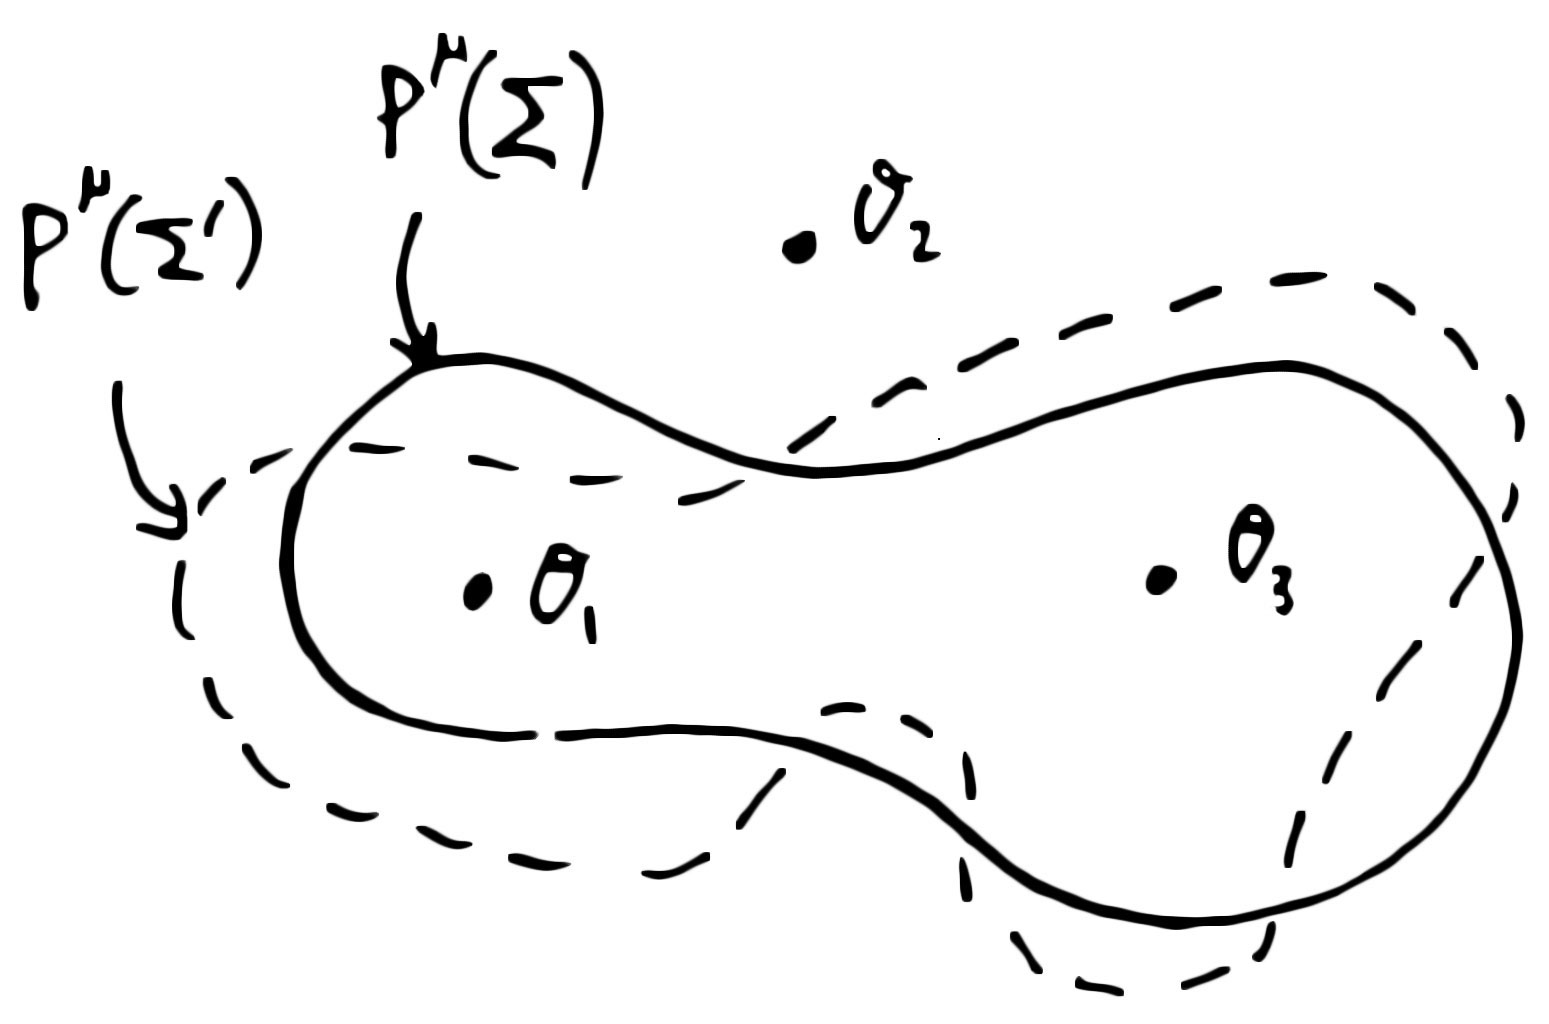
\includegraphics[width=0.45\textwidth]{topologicalsurfaces.jpg}
\end{center}
\caption{A surface $\Sigma$ supporting the operator $P^\mu(\Sigma)$ can be freely deformed $\Sigma\to\Sigma'$ without changing the correlation function, as long as it doesn't cross any operator insertions.
\label{fig:topologicalsurfaces} }
\end{figure}

Let $\Sigma=\ptl B$ be the boundary of a ball $B$ containing $x$ and no other insertions. Integrating (\ref{eq:wardidentity}) over $B$ gives
\be
\label{eq:integratedwardidentity}
\<P^\mu(\Sigma)\cO(x)\dots\> &= \ptl^\mu\<\cO(x)\dots\>.
\ee
In other words, surrounding $\cO(x)$ with the topological surface operator $P^\mu$ is equivalent to taking a derivative (figure~\ref{fig:surroundoperator}).

\begin{figure}
\begin{center}
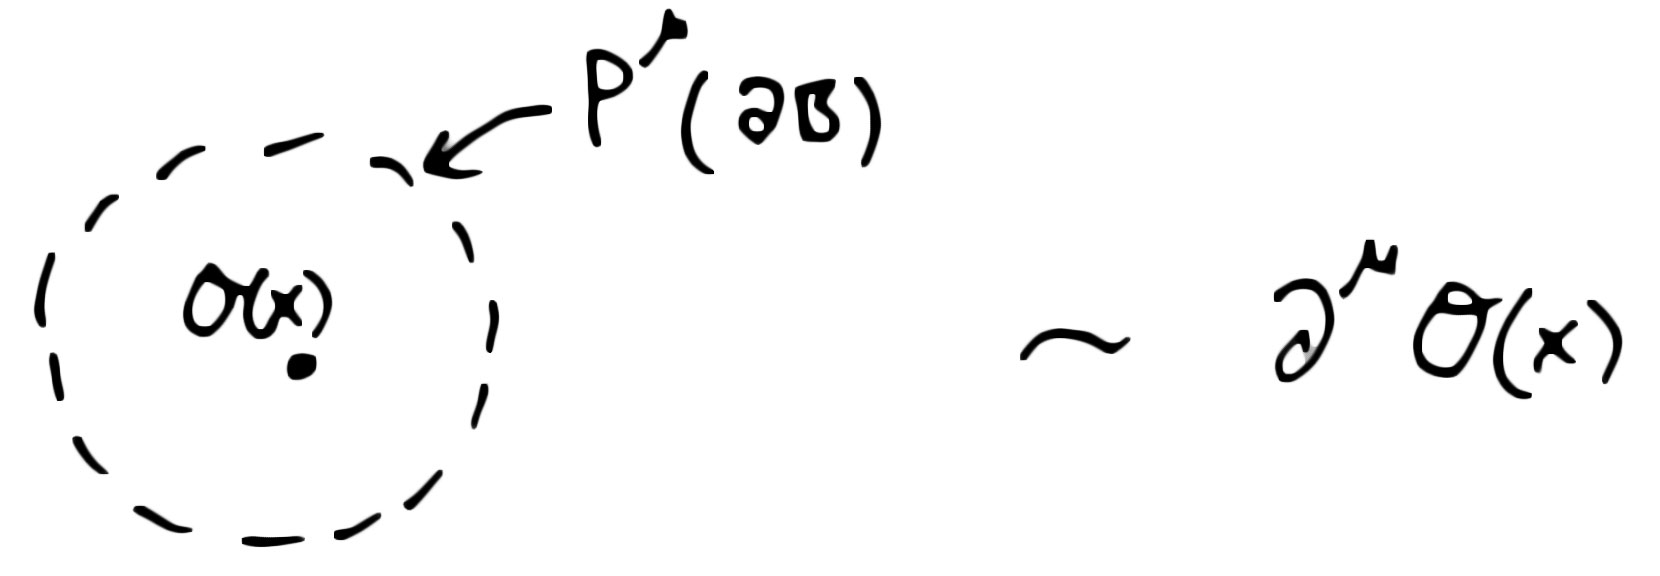
\includegraphics[width=0.5\textwidth]{surroundoperator.jpg}
\end{center}
\caption{\label{fig:surroundoperator} Surrounding $\cO(x)$ with $P^\mu$ gives a derivative.}
\end{figure}

In quantum field theory, having a topological codimension-1 operator is the same as having a symmetry.\footnote{Topological operators with support on other types of manifolds give ``generalized symmetries" \cite{Gaiotto:2014kfa}.}${}^,$\footnote{More precisely, to have a symmetry we usually require the topological codimension-1 operators to be invertible. If they are group-like, this means they have a multiplicative inverse, and if they are algebra-like, they have an additive inverse.}  This may be unfamiliar language, so to connect to something more familiar, let us revisit the relation between the path integral and Hamiltonian formalisms.

%
%\subsection{Quantization}
%\label{sec:quantization}
%
%A single path integral can be interpreted in terms of different time evolutions in different Hilbert spaces.  For example, in a rotationally-invariant Euclidean theory on $\R^d$, we can choose any direction as ``time" and think of states living on slices orthogonal to the time direction (figure~\ref{fig:differentquantizations}).  We call each interpretation a ``quantization" of the theory.


%
%To specify a quantization, we foliate spacetime by slices related by an isometry $\ptl_t$. A slice has an associated Hilbert space of states.  A correlation function $\<\cO_1(x_1)\cdots\cO_n(x_2)\>$ gets interpreted as a time-ordered expectation value
%\be
%\label{eq:timeordered}
%\<\cO_1(x_1)\cdots\cO_n(x_n)\> &= \<0|T\{\widehat \cO_1(t_1,\bx_1)\cdots \widehat \cO_n(t_n,\bx_n)\}|0\>.
%\ee
%Here, the time ordering $T\{\dots\}$ is with respect to our foliation, $|0\>$ is the vacuum in the Hilbert space $\cH$ living on a spatial slice,\footnote{Other choices of initial and final state correspond to different boundary conditions for the path integral.} and $\widehat\cO_i(x):\cH\to \cH$ are quantum operators corresponding to the path integral insertions $\cO_i(x)$.
  
%A different quantization of the theory would give a completely different Hilbert space $\cH'$, a completely different time-ordering, and completely different quantum operators $\widehat \cO_i'$.  However, some equations satisfied by these new operators on this new Hilbert space would be unchanged.  For example, if we arrange the operators as shown on the right-hand side of (\ref{eq:timeordered}), we always get the correlator on the left-hand side.
%
%We demonstrate these ideas explicitly in appendix~\ref{app:latticequantization}, where we show how to (discretely) quantize the lattice Ising model in different ways.


\begin{figure}
\begin{center}
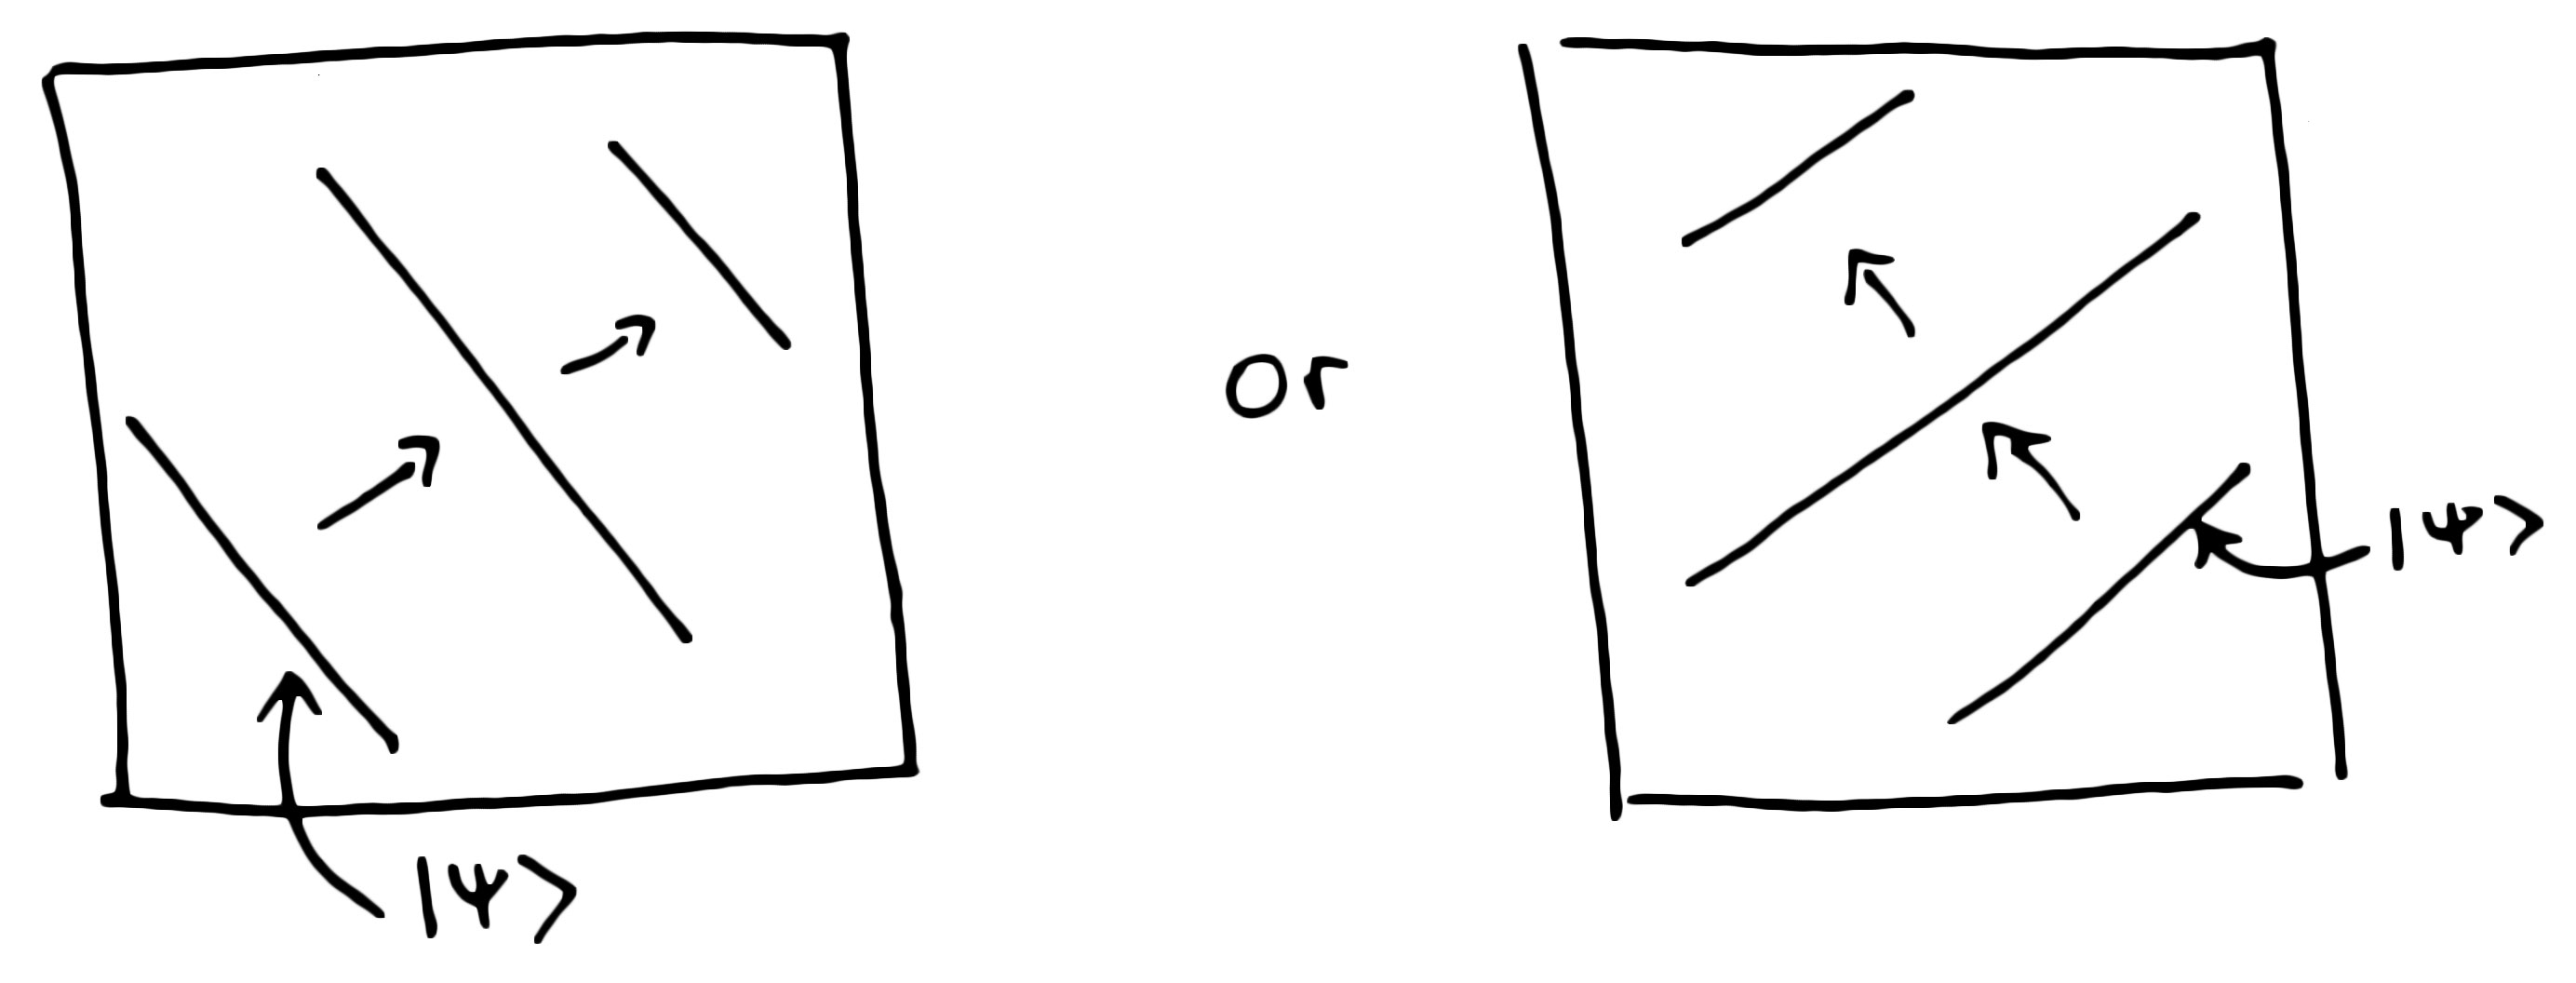
\includegraphics[width=0.65\textwidth]{differentquantizations.jpg}
\end{center}
\caption{\label{fig:differentquantizations} In a rotationally invariant Euclidean theory, we can choose any direction as time.  States live on slices orthogonal to the time direction.}
\end{figure}

Recall that the path integral can be interpreted in terms of different quantizations. To specify a quantization, we foliate spacetime by slices related by an isometry $\ptl_t$ (figure~\ref{fig:differentquantizations}). A slice has an associated Hilbert space of states.  A correlation function $\<\cO_1(x_1)\cdots\cO_n(x_2)\>$ gets interpreted as a time-ordered expectation value
\be
\label{eq:timeordered}
\<\cO_1(x_1)\cdots\cO_n(x_n)\> &= \<0|T\{\widehat \cO_1(t_1,\bx_1)\cdots \widehat \cO_n(t_n,\bx_n)\}|0\>.
\ee
Here, the time ordering $T\{\dots\}$ is with respect to our foliation, $|0\>$ is the vacuum in the Hilbert space $\cH$ living on a spatial slice,\footnote{Other choices of initial and final state correspond to different boundary conditions for the path integral.} and $\widehat\cO_i(x):\cH\to \cH$ are quantum operators corresponding to the path integral insertions $\cO_i(x)$.

\begin{figure}
\begin{center}
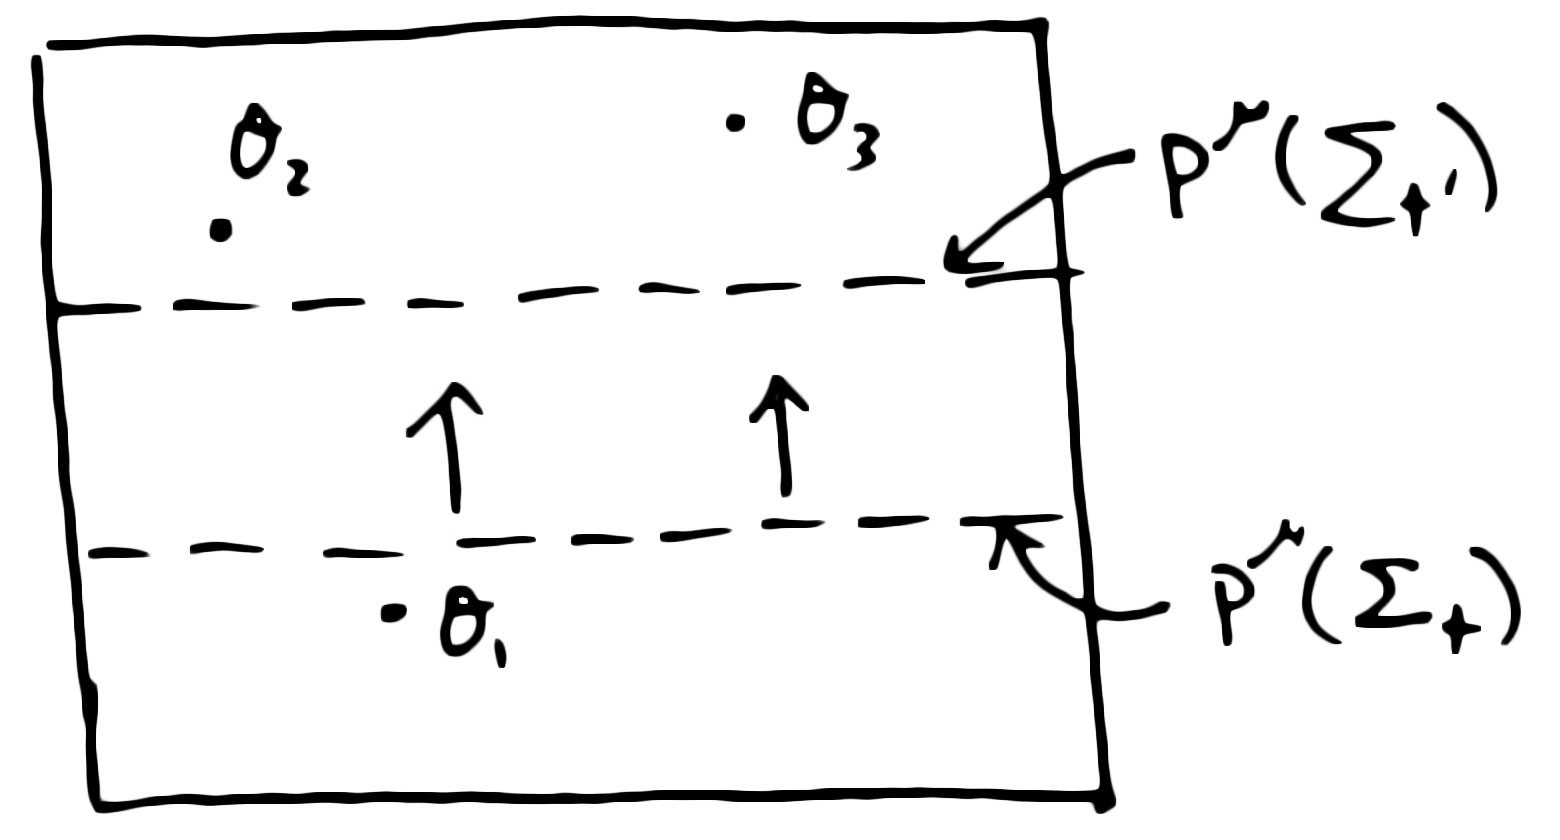
\includegraphics[width=0.5\textwidth]{slidingcharges.jpg}
\end{center}
\caption{\label{fig:slidingcharges} The charge $P^\mu(\Sigma_t)$ can be moved from one time to another $t\to t'$ without changing the correlation function.}
\end{figure}

Let $\Sigma_t$ be a spatial slice at time $t$ and consider the operator $P^\mu(\Sigma_t)$.  Because $P^\mu(\Sigma)$ is topological, we are free to move it forward or backward in time from one spatial slice to another as long as it doesn't cross any operator insertions (figure~\ref{fig:slidingcharges}). In fact, we  often neglect to specify the surface $\Sigma_t$ and just write $P^\mu$ (though we should keep in mind where the surface lives with respect to other operators). We call $P^\mu$ ``momentum," and the fact that it's topological is the path integral version of the statement that momentum is conserved.

Let us understand what happens when we move $P^\mu$ past an operator insertion. Consider a local operator $\cO(x)$ at time $t$. If $\Sigma_1$, $\Sigma_2$ are spatial surfaces at times $t_1<t<t_2$, then when we quantize our theory, the difference $P^\mu(\Sigma_{2})-P^\mu(\Sigma_{1})$ becomes a commutator because of time ordering,
\be
\<(P^\mu(\Sigma_{2})-P^\mu(\Sigma_{1}))\cO(x)\dots\>=\<0|T\{[\widehat P^\mu,\widehat \cO(x)]\dots\}|0\>.
\ee
(We assume that the other insertions ``$\dots$" are not between times $t_1$ and $t_2$.)
Because $P^\mu$ is topological, we can deform $\Sigma_2-\Sigma_1$ to a sphere $S$ surrounding $\cO(x)$, as in figure~\ref{fig:deformingcharges}.  Then using the Ward identity (\ref{eq:integratedwardidentity}), we find
\be
\<0|T\{[\widehat P^\mu, \widehat \cO(x)]\dots\}|0\>&=\<(P^\mu(\Sigma_2)-P^\mu(\Sigma_1))\cO(x)\dots\>\nn\\
&=\<P^\mu(S)\cO(x)\dots\>\nn\\
&= \ptl^\mu\<\cO(x)\dots\>\nn\\
&= \ptl^\mu\<0|T\{\widehat \cO(x)\dots\}|0\>,
\ee
in other words,
\be
[\widehat P^\mu, \widehat \cO(x)] &= \ptl^\mu\widehat \cO(x).
\ee

\begin{figure}
\begin{center}
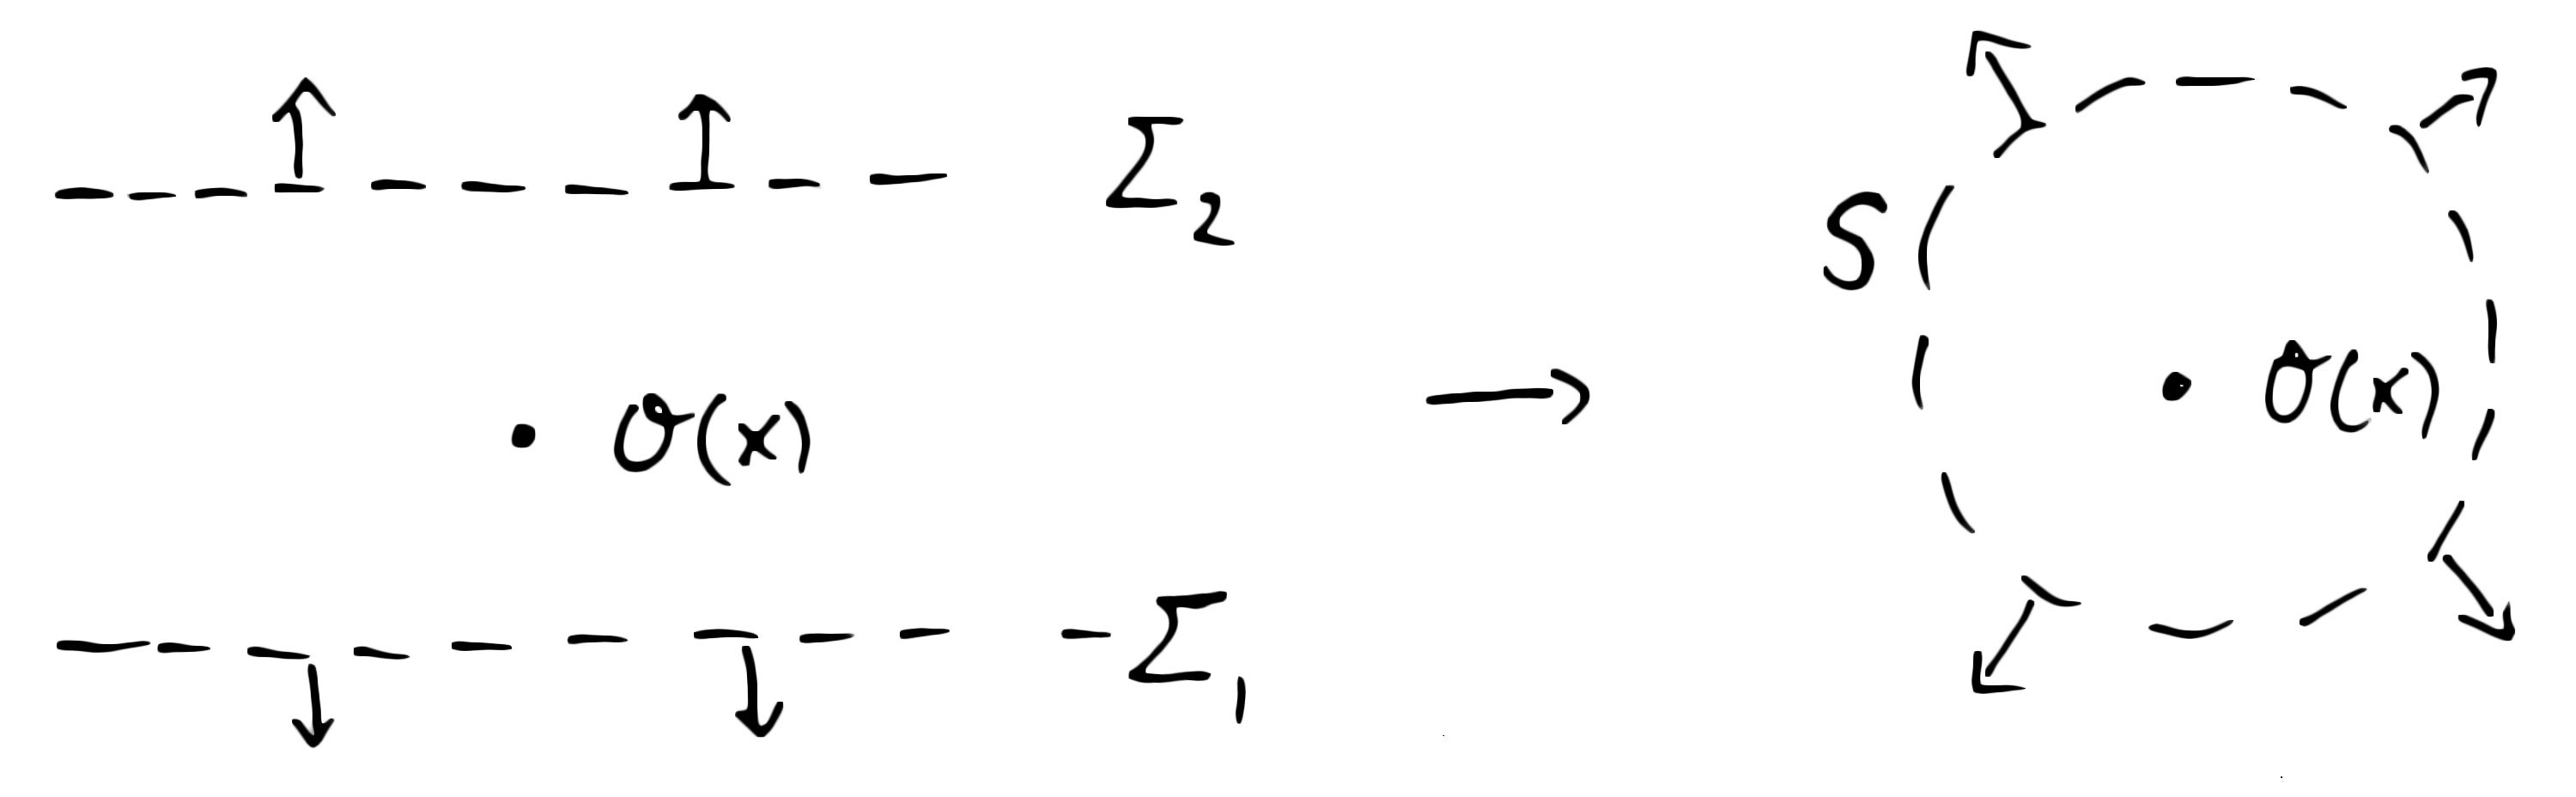
\includegraphics[width=0.8\textwidth]{deformingcharges.jpg}
\end{center}
\caption{\label{fig:deformingcharges} For any charge $Q(\Sigma)$, we can deform $Q(\Sigma_2)-Q(\Sigma_1)=Q(\Sigma_2-\Sigma_1)$ to an insertion of $Q(S)$. Here, arrows indicate the orientation of the surface.}
\end{figure}

Figure~\ref{fig:deformingcharges} makes it clear that this result is independent of how we quantize our theory, since we always obtain a sphere surrounding $\cO(x)$ no matter which direction we choose as ``time."  Thus, we often write
\be
\label{commutator}
[P^\mu,\cO(x)] &= \ptl^\mu\cO(x),
\ee
without specifying a quantization.  In fact, from now on, we will no longer distinguish between path integral insertions $\cO(x)$ and quantum operators $\widehat \cO(x)$.
The expression $[Q,\cO(x)]$ can be interpreted as either an actual commutator $[\widehat Q,\widehat \cO(x)]$ in any quantization of the theory, or in path-integral language as surrounding $\cO(x)$ with a topological surface operator $Q(S)$.

Figure~\ref{fig:deformingcharges} also explains why the commutator $[Q,\cO(x)]$ of a charge $Q$ with a local operator $\cO(x)$ is local, even though $Q$ is nonlocal (it is the integral of a current). The reason is that the support of $Q$ can be deformed to an arbitrarily small sphere $S$ around $x$, so that the insertion $Q(S)\cO(x)$ only affects the path integral in an infinitesimal neighborhood of $x$.  In general, the way local operators transform under symmetry is always insensitive to IR details like spontaneous symmetry breaking or finite temperature.  This is because commutators with conserved charges can be computed at short distances.

\stoplecture

Equation (\ref{commutator}) integrates to
\be
\label{eq:integratedtranslations}
\cO(x) &= e^{x\.P}\cO(0)e^{-x\.P}.
\ee
This statement is also true in any quantization of the theory.  In path integral language, $e^{x\.P}(\Sigma)$ is another type of topological surface operator.  When we surround $\cO(0)$ with $e^{x\.P}(\Sigma)$, it becomes conjugation $e^{x\.P}(\Sigma)\cO(0)\to e^{\widehat P\. x}\widehat\cO(0)e^{- \widehat P\. x}$ in any quantization.

Consider the time-ordered correlator (\ref{eq:timeordered}) with $t_n>\cdots>t_1$.  Using (\ref{eq:integratedtranslations}), it becomes
\begin{align}
&\<\cO_1(x_1)\cdots\cO_n(x_n)\>\nonumber\\
&= \<0|e^{t_n P^0}\cO_n(0,\bx_n)e^{-t_n P^0}\cdots e^{t_1 P^0}\cO_1(0,\bx_1)e^{-t_1P^0}|0\>\nonumber\\
&=\<0|\cO_n(0,\bx_n)e^{-(t_n-t_{n-1})P^0}\cdots e^{-(t_2-t_1)P^0}\cO_1(0,\bx_1)|0\>.
\end{align}
In other words, the path integral between spatial slices separated by time $t$ computes a time evolution operator $U(t)=e^{-tP^0}$. In particular, $P^0$ is the Hamiltonian, as expected.  %In unitary theories (defined in more detail in section~\ref{sec:reflectionpositivity}), $P^0$ has a positive real spectrum, so $U(t)$ causes damping at large time separations.

\subsection{A topological surface operator on the lattice}

Let us give an example of a topological surface operator that is not the integral of a current (or the  exponential of the integral of a current). We will again see that it should be thought of as a symmetry.

Consider the lattice Ising model in $d$-dimensions with zero applied magnetic field, $h=0$. The operator $U_{\Z_2}(\Sigma)$ is defined by flipping the signs of all nearest-neighbor bonds that cross the surface $\Sigma$. More precisely, let $\Sigma$ be a closed surface that does not intersect any of the lattice points. For each pair of nearest neighbor sites $\<ij\>$, define the sign\footnote{Being more careful to allow for very wiggly surfaces, we should define $p_\Sigma(i,j)$ as $(-1)^n$, where $n$ is the number of times $\Sigma$ intersects the edge $\<ij\>$.}
\be
p_{i,j}(\Sigma) &= \begin{cases}
-1 & \textrm{if the edge from $i$ to $j$ intersects $\Sigma$,} \nn\\
+1 & \textrm{otherwise}.
\end{cases}
\ee
An insertion of $U_{\Z_2}(\Sigma)$ is defined by
\be
\label{eq:pathintegralwithUinserted}
\<U_{\Z_2}(\Sigma) \cO_1\cdots \cO_n \> &\equiv \sum_{\{s_i\}}  \cO_1\cdots \cO_n e^{K\sum_{\<ij\>} p_{i,j}(\Sigma) s_i s_j}.
\ee

Why is the operator $U_{\Z_2}(\Sigma)$ topological? Consider a deformation $\Sigma\to \Sigma'$. Because $\Sigma$ and $\Sigma'$ are homologous, their difference is the boundary of a region $\mathcal{R}$, i.e.\ $\ptl\mathcal{R}=\Sigma-\Sigma'$. We can transform $U_{\Z_2}(\Sigma)$ into $U_{\Z_2}(\Sigma')$ by doing a change of variables $s_i\to -s_i$ in the path integral (\ref{eq:pathintegralwithUinserted}) for all spins in $\mathcal{R}$.

When we flip the spins in $\mathcal{R}$, any $\Z_2$-odd operator in that region will also flip sign. Thus, $U_{\Z_2}(\Sigma)$ can be deformed freely, but when we move it past an operator, we pick up the $\Z_2$ charge of that operator. For example, if $B$ is a ball containing an operator $\cO$ (and no other operators), we have
\be
\label{eq:ztsphere}
\<U_{\Z_2}(\ptl B) \cO \cdots\> &= q_\cO\< \cO\cdots\>,\qquad q_\cO=\pm 1.
\ee
This equation is exactly analogous to (\ref{eq:integratedwardidentity}).

Consider inserting $U_{\mathbb{Z}_2}$ on a spatial slice $\Sigma_t$ at fixed time $t$.\footnote{Since we are on a lattice, $t$ is discrete. As usual, we are free to choose any lattice direction as time.} After quantization, $U_{\mathbb{Z}_2}(\Sigma_t)$ becomes an operator $\hat U_{\mathbb{Z}_2}$ that is independent of $t$ (i.e.\ conserved) because $U_{\mathbb{Z}_2}$ is topological. The only effect of $t$ is to determine the ordering of quantum operators. For example, assuming $t_3>t_2>t_1$, we have\footnote{When $\Sigma$ is inserted between two rows of spins, we evolve from one row to the next using either $\hat T \hat U_{\mathbb{Z}_2}$ or $ \hat U_{\mathbb{Z}_2}\hat T$, where $\hat T$ is the transfer matrix. The two choices are the same because $\hat U_{\mathbb{Z}_2}$ commutes with $\hat T$. This is one way of saying that $\hat U_{\mathbb{Z}_2}$ is conserved.}
\be
\<\cO_3(t_3) U_{\Z_2}(\Sigma_{t_2}) \cO_1(t_1)\> &= \<0|\hat \cO_3(t_3) \hat U_{\mathbb{Z}_2} \hat \cO_1(t_1)|0\>.
\ee
Here $\hat \cO_i(t_i)$ are Heisenberg-picture operators as in, e.g.\ (\ref{eq:oldspinop}). The statement (\ref{eq:ztsphere}) is equivalent to
\be
\label{eq:commutatordiscrete}
\hat U_{\mathbb{Z}_2} \hat \cO \hat U_{\mathbb{Z}_2}^{-1} &= q_\cO \hat \cO.
\ee
Concretely, the operator $\hat U_{\mathbb{Z}_2}$ is given by
\be
\hat U_{\mathbb{Z}_2} = \prod_{i=1}^M \s^x_i,\qquad \hat U_{\mathbb{Z}_2}|\bs\> = |-\bs\>.
\ee
where $\bs=(s_1,\cdots, s_M)$ are the spins on a spatial slice.

By now it should be clear that $\hat U_{\mathbb{Z}_2}$ is the generator of a $\mathbb{Z}_2$ global symmetry acting on the Hilbert space. The path integral perspective shows that we can consider $U_{\mathbb{Z}_2}$ on surfaces other than just spatial slices.% This often makes symmetries more manifest.% For example from the definition (\ref{eq:uassigmaxs}), it is not clear why (\ref{eq:commutatordiscrete}) should be a local operator. However, this is obvious from the fact that $U_{\mathbb{Z}_2}(\Sigma)$ is topological, since we can take $\Sigma$ to be a very small sphere surrounding $\cO$.

\subsubsection{Implementation in the continuum}

The operator $U_{\mathbb{Z}_2}$ can also be defined in continuum $\f^4$ theory as follows. Given a surface $\Sigma$, let us cover space with small open balls $B_i$ such that $\Sigma$ splits each ball into at most two pieces $B_i^\mathrm{left}\cup B_i^\mathrm{right}$ (one of which might be empty). We do this so we don't have to  worry about the global structure of $\Sigma$. The action without an insertion of $U_{\mathbb{Z}_2}(\Sigma)$ can be written as
\be
S[\phi] &= \sum_{i} \int_{B_i} d^d x  f_i(x) \cL[\f](x),\nn\\
\cL[\phi](x) &= \frac 1 2 (\ptl \f)^2 + \dots,
\ee
where $f_i(x)$ is a partition of unity for the balls $B_i$. This means that $f_i$ are functions such that $f_i$ is supported inside $B_i$ and $\sum_i f_i = 1$.
Note that $S[\phi]$ favors configurations where $\f$ is slowly-varying.

To insert $U_{\mathbb{Z}_2}(\Sigma)$, we would like to instead favor configurations where $\f$ flips sign as it crosses $\Sigma$. Let 
\be
\f_i'(x) &= \begin{cases} 
\f(x) & x\in B_i^\mathrm{right} \nn\\
-\f(x) & x\in B_i^\mathrm{left}
\end{cases}.
\ee
The modified action is given by
\be
S'[\phi] &= \sum_i\int_{B_i} d^d x f_i(x) \cL[\f'_i](x).
\ee
Inserting $U_{\mathbb{Z}_2}(\Sigma)$ means performing the path integral with the modified action $S'$,
\be
\<U_{\mathbb{Z}_2}(\Sigma) \cO_1\cdots \cO_n\> &= \int D\f\, \cO_1\cdots \cO_n e^{-S'[\f]}.
\ee
This is the continuum version of flipping the bonds that cross $\Sigma$. 

In practice, it is difficult to work with $S'[\f]$ because it has funny $\de$-functions coming from  derivatives of $\f'$. If $\Sigma=\ptl B$ is the boundary of a region $B$, we can make a change of variables $\f\to -\f$ inside $B$ to get rid of $U_{\mathbb{Z}_2}(\Sigma)$. When we do this, any $\Z_2$-odd operator inside $B$ will pick up a sign. This gives the same result (\ref{eq:ztsphere}) that we found on the lattice.

However, if $\Sigma$ is not the boundary of a region, we cannot make a change of variables to remove $U_{\mathbb{Z}_2}(\Sigma)$. As an example, consider the theory on a torus $T^d$ with $U_{\mathbb{Z}_2}$ inserted on a spatial slice $T^{d-1}\subset T^d$. This slice is homologically nontrivial, so no change of variables will remove $U_{\mathbb{Z}_2}$. However, we can simplify the action by defining $\f$ to flip sign as we cross $\Sigma$,
\be
\f(t_\mathrm{below}) = -\f(t_\mathrm{above}).
\ee
This turns $S'$ back into $S$, but with the cost of introducing ``twisted" boundary conditions for the field $\f$
\be
\label{eq:antiperiodicity}
\f(t+\b) &= -\f(t),
\ee
where $\b$ is the length of the time circle. The path integral with twisted boundary conditions is often more straightforward to evaluate.

One effect of inserting $U_{\mathbb{Z}_2}$ on a spatial slice $T^{d-1}\subset T^d$ is that correlators of $\Z_2$-odd operators in the presence of $U_{\mathbb{Z}_2}(T^{d-1})$ become antiperiodic in the time direction. This is because to move them around the time circle, we must cross $U_{\mathbb{Z}_2}$, and doing so introduces a sign. This can also be understood in terms of twisted boundary conditions: any operator made of an odd number of $\f$'s will be antiperiodic because of (\ref{eq:antiperiodicity}).

\subsection{More spacetime symmetries}

Let us return to discussing symmetries built from the stress tensor. Given a conserved current $\ptl_\mu J^\mu=0$ (as an operator equation), we can always define a topological surface operator by integration.\footnote{It is an interesting question whether the converse is true. When a theory has a Lagrangian description, the Noether procedure gives a conserved current for any continuous symmetry (that is manifest in the Lagrangian).  Proving Noether's theorem without a Lagrangian is an open problem.} For $P^\nu$, the corresponding currents are $T^{\mu\nu}(x)$.  More generally, given a vector field $\e=\e^\mu(x)\ptl_\mu$, the charge
\be
Q_\e(\Sigma) &= -\int_\Sigma dS_\mu \e_\nu(x) T^{\mu\nu}(x)
\ee
will be conserved whenever
\be
0&=\ptl_\mu(\e_\nu T^{\mu\nu}) \nn\\
&=
 \ptl_\mu \e_\nu T^{\mu\nu}+\e_\nu \ptl_\mu T^{\mu\nu}\nn\\
&= \frac 1 2(\ptl_\mu \e_\nu+\ptl_\nu \e_\mu) T^{\mu\nu},
\ee
or
\be
\label{eq:killingvector}
\ptl_\mu\e_\nu+\ptl_\nu\e_\mu &= 0.
\ee
This is the Killing equation. It is equivalent to the statement that $\e$ generates an isometry of the flat metric on $\R^d$. It has solutions
\begin{align}
\label{eq:poincaregenerators}
p_\mu &= \ptl_\mu &\textrm{(translations)},\nn\\
m_{\mu\nu} &= x_\nu\ptl_\mu - x_\mu\ptl_\nu & \textrm{(rotations)}.
\end{align}
The corresponding charges
are momentum $P_\mu=Q_{p_\mu}$ and angular momentum $M_{\mu\nu}=Q_{m_{\mu\nu}}$.

\stoplecture

\section{Conformal symmetry}

In a conformal field theory, the stress tensor satisfies an additional condition: it is traceless,
\be
T_\mu^\mu(x) &= 0 \qquad\textrm{(operator equation)}.
\ee
This is equivalent to the statement that the theory is insensitive to position-dependent rescalings of the metric $\de g_{\mu\nu}=2\omega(x) g_{\mu\nu}$ near flat space.\footnote{In curved space, there can by Weyl anomalies, which we discuss in section~\ref{}.} %Tracelessness of $T_{\mu\nu}$ is our final CFT axiom:
%\begin{definition}
%A conformal field theory (CFT) is a QFT satisfying the Atiyah-Segal axioms discussed in section~\ref{sec:asaxioms}, and possessing a conserved, symmetric, traceless stress tensor.
%\end{definition}

\subsection{Scale-invariance plus unitarity implies conformal invariance in 2d}
\label{sec:scaleimpliesconformal}

We have seen that critical points exhibit scale-invariance, but it might not be obvious why they should have a traceless stress tensor. Proving that scale-invariance implies $T_\mu^\mu=0$ for general $d$ is an open problem.\footnote{An almost-complete argument exists in 4-dimensions \cite{}. Part of the challenge is identifying the appropriate assumptions to make. There exist boring/pathological counterexamples in 3d (for example free electromagnetism), and the right formulation of the theorem should exclude these cases.} However, proving it for $d=2$ is straightforward.\footnote{This argument is from Zohar Komargodski's notes \cite{KomargodskiNotes}. See \cite{YellowPages} for a similar proof in position-space.}

Consider the two-point function of the stress tensor in momentum space (this will make it easy to study conservation). Symmetry and conservation require it to take the form
\be
\label{eq:momentumspacetwopt}
\<T_{\mu\nu}(q) T_{\rho \s}(-q)\> &= \frac 1 2 ((q_\mu q_\rho - q^2 \de_{\mu \rho})(q_\nu q_\s - q^2 \de_{\nu\s}) + \rho \leftrightarrow \s) f(q^2)\nn\\
&\qquad + (q_\mu q_\nu - q^2 \de_{\mu\nu})(q_\rho q_\s - q^2 \de_{\rho \s}) g(q^2),
\ee
where $f(q^2)$, $g(q^2)$ are general functions of $q^2$. Here, we have Fourier transformed the two operators with momenta $p,q$, and stripped off an overall momentum-conserving $\de^d(p+q)$.

The form (\ref{eq:momentumspacetwopt}) holds in any $d$. However in $d=2$, something special happens: the two structures above are linearly-dependent.
\begin{exercise}
Let $d=2$, and consider $\tl q_\mu = \e_{\mu\nu} q^\nu$, where $\e_{\mu\nu}$ is the totally antisymmetric symbol:
\be
\e_{01} = 1,\quad \e_{10}=-1,\quad \e_{00}=\e_{11}=0.
\ee
Simplify the product
\be
\tl q_{\mu} \tl q_\nu \tl q_\rho \tl q_\s
\ee
in two different ways to obtain the structures multiplying $f(q^2)$ and $g(q^2)$.
\end{exercise}

Thus, in two dimensions, we have simply
\be
\label{eq:twoptmomentum2d}
\<T_{\mu\nu}(q) T_{\rho \s}(-q)\> &=(q_\mu q_\nu - q^2 \de_{\mu\nu})(q_\rho q_\s - q^2 \de_{\rho \s}) h(q^2)
\ee
for a single function $h(q^2)$.
Now suppose that the theory is also scale-invariant. This implies that $h(q^2)$ should be a pure power of $q$,\footnote{Nontrivial scale-dependence is allowed in correlation functions if it multiplies a contact term (i.e.\ the violation of scaling is invisible at separated points). In momentum space, this means we can have terms proportional to $\log(q^2/\mu^2)$, provided they multiply an analytic function of $q$ (whose Fourier transform is a contact term). In the case of $h(q^2)$, something like $q^{-2} \log(q^2/\mu^2)$ is disallowed because $\mu\frac{d}{d\mu} q^{-2} \log(q^2/\mu^2)$ is not analytic in $q$.}
\be
h(q^2) &= \frac{b}{q^2}.
\ee
The dimension of $h(q^2)$ comes from the fact that $T_{\mu\nu}(q)$ is dimensionless (it is the $d$-dimensional Fourier transform of a quantity with dimension $d$), but we have also stripped off a dimensionful $\de^d(p+q)$ to define (\ref{eq:twoptmomentum2d}).
Taking the trace, we find
\be
\<T(q) T(-q)\> &= b q^2,
\ee
where $T\equiv T^\mu_\mu$.
In position-space, this becomes a contact term
\be
\<T(x) T(y)\> &\propto b\ptl^2 \de^2(x-y).
\ee

%In a 2d scale-invariant theory, the stress tensor is a spin-2 operator with scaling dimension $2$. The most general two-point function consistent with these properties, together with Poincare-invariance and permutation symmetry is
%\be
%\<T_{\mu\nu}(x)T_{\rho\s}(0)\> &= \frac{1}{x^8} \left(A_1 \de_{\mu\nu}\de_{\rho \s} x^4 + A_2 (\de_{\mu\rho} \de_{\nu\s}+ \de_{\mu\s}\de_{\nu\rho}) x^4\right.\nn\\
%&\qquad\quad \left.+ A_3 (\de_{\mu\nu} x_\rho x_\s + \de_{\rho\s}x_\mu x_\nu)x^2 + A_4 x_\mu x_\nu x_\rho x_\s)\right),
%\ee
%where the $A_i$'s are constants.
%Conservation then implies
%\be
%\ptl^\mu\<T_{\mu\nu}(x)T_{\rho\s}(0)\> &= -\frac{1}{x^8} \left(3(A_4+2A_3)x_\nu x_\rho x_\s + (4A_1+3A_3)\de_{\rho\s} x_\nu x^2\right.\nn\\
%&\qquad\qquad \left.+ (4A_2-A_3)(\de_{\rho\nu} x_\s + \de_{\nu\s}x_\rho)\right),
%\ee
%which means $A_1,A_2,A_3,A_4$ are determined in terms of a single constant
%\be
%A_1 = 3A,\quad A_2 = -A,\quad A_3 = -4A,\quad A_4=8A.
%\ee
%The two-point function becomes
%\be
%\<T_{\mu\nu}(x)T_{\rho\s}(0)\> &= \frac{A}{x^8} \left((3 \de_{\mu\nu}\de_{\rho\s} - \de_{\mu\rho}\de_{\nu\s} - \de_{\mu\s}\de_{\nu\rho}) x^4 \right.\nn\\
%&\qquad\quad \left.-4x^2(\de_{\mu\nu}x_\rho x_\s + \de_{\rho\s} x_\mu x_\nu) + 8x_\mu x_\nu x_\rho x_\s\right).
%\ee
%Taking the trace, we find
%\be
%\<T(x) T(0)\> &= 0,
%\ee
%where $T(x)\equiv T^\mu_\mu(x)$.

In a unitary quantum field theory, if the two point function of an operator vanishes at separated points, {\it any\/} correlator involving that operator vanishes at separated points. Roughly-speaking, unitary means the theory that can be quantized in such a way that the space of states has a positive-definite inner product and the Hamiltonian is Hermitian and bounded from below. In a Euclidean theory, a more correct term is ``reflection positivity." We will discuss unitarity/reflection positivity in more detail later.

The argument for vanishing of $T(x)$ is as follows. As we discussed in the introduction, in a unitary theory, inserting a complete set of states into a two-point function gives a sum of positive terms (see equation~(\ref{eq:completeset}))
\be
\label{eq:positivesumforttwopt}
\<T(x^0,\mathbf{ 0})T(0)\> &= \sum_\psi |\<0|T(0)|\psi\>|^2 e^{-E_\psi x^0}.
\ee
If the left-hand side vanishes, each term on the right-hand side must vanish as well: $\<0|T(0)|\psi\>=0$, in other words $T(x)$ must annihilate the vacuum. Now consider a general correlation function of $T(x)$ with other operators,
\be
\label{eq:correlatorofTwithstuff}
\<T(x) \cO_1(x_1)\cdots \cO_n(x_n)\>.
\ee
This correlator vanishes if $x$ is in the past or future of all the other $x_i$, since then $T(x)$ acts on the vacuum on either the right or left. However, correlation functions in QFT are analytic in their arguments, and the analytic continuation of zero is zero. Thus, the entire correlator (\ref{eq:correlatorofTwithstuff}) vanishes.

\subsubsection{Scale without conformal invariance}

Scale without conformal invariance is possible in nonunitary theories. Perhaps the simplest example is the theory of elasticity in 2 dimensions \cite{Riva:2005gd}. This is the theory of a vector $u_\mu$ with action
\be
\label{eq:theoryofelasticity}
S &= \int d^2 x \p{g u_{\mu\nu} u^{\mu\nu} + \frac k 2 (u_\mu{}^\mu)^2},
\ee
where $u_{\mu\nu}=\frac 1 2 (\ptl_\mu u_\nu + \ptl_\nu u_\mu)$. The field $u_\mu$ is called the ``displacement field" and $u_{\mu\nu}$ is called the ``strain tensor." The coefficient $g$ represents the shear modulus, and $k+g$ is the bulk modulus of the described material.

The action (\ref{eq:theoryofelasticity}) is quadratic in $u$, so this theory is easy to quantize. Note that $u_\mu$ describes a massless vector field without a gauge redundancy. Thus, there are negative-norm states, and the theory is nonunitary. Concretely, one can define a conserved stress tensor $T^{\mu\nu}$ that satisfies the correct Ward identities, and such that $\<T_\mu^\mu T_\nu^\nu\>=0$, but $T_\mu^\mu$ is not zero. For example, it has non-vanishing correlation functions with other operators:
\be
\<T_\mu^\mu(z) :\!\ptl u \ptl u\!:\!(0)\> &= -\frac{k+g}{2\pi^2 g(k+2g)} \frac{1}{z^4}.
\ee
(Here, we use complex coordinates $z=x+iy$ and $u=u_1-i u_2$.)

This example shows that the positive sum (\ref{eq:positivesumforttwopt}) for $\<TT\>$ is crucial for completing the argument in section~\ref{sec:scaleimpliesconformal}. The proof that scale implies conformal invariance in 4d \cite{} also uses unitarity in a fundamental way. However, though unitarity may be a sufficient condition for conformal invariance, it is not necessary. We will encounter some interesting nonunitary CFTs (like the Lee-Yang theory) later in the course.

\draftnote{Discuss virial current?}

\subsection{Symmetries from tracelessness}

Recall that the charge $Q_\e(\Sigma)$ is conserved if
\be
 \frac 1 2(\ptl_\mu \e_\nu+\ptl_\nu \e_\mu) T^{\mu\nu} &= 0.
 \ee
 When the stress tensor is traceless, this condition can be solved by demanding a less constraining version of the Killing equation (\ref{eq:killingvector}),
\be
\label{eq:conformalkillingfirst}
\ptl_\mu\e_\nu + \ptl_\nu \e_\mu = c(x)\de_{\mu\nu},
\ee
where $c(x)$ is any scalar function.  Contracting both sides with $\de^{\mu\nu}$ determines $c$ in terms of $\e$,
\be
\label{eq:conformalkilling}
\ptl_\mu\e_\nu + \ptl_\nu \e_\mu = \frac{2}{d}(\ptl \. \e)\de_{\mu\nu}.
\ee

Equation (\ref{eq:conformalkilling}) is the {\it conformal\/} Killing equation. Let us find its solutions in $\R^d$. Taking $\ptl^\nu\ptl^\mu$ of both sides, we find
\be
\label{eq:termneededforvirasoro}
\p{2-\frac 2 d} \ptl^2(\ptl\.\e) = 0\quad \implies \quad \ptl^2 (\ptl \. \e)=0,
\ee
where we have assumed that $d\neq 1$. Now taking $\ptl^\nu\ptl_\rho$ and symmetrizing in $(\rho\mu)$, we find
\be
\p{1-\frac{2}{d}}\ptl_\rho\ptl_\mu(\ptl \. \e)=0 %\quad\implies\quad \ptl_\rho \ptl_\mu(\ptl\.\e) = 0\textrm{ or $d=2$}.
\label{eq:equationaboutdivergence}
\ee
For the moment, let us focus on the case $d\neq 2$, so we can conclude that $\ptl_\rho \ptl_\mu(\ptl\.\e)=0$. Taking two derivatives of the conformal Killing equation and using (\ref{eq:equationaboutdivergence}), we find
\be
\ptl_\a(\ptl_\b \ptl_\g \e_\de + \ptl_\b \ptl_\de \e_\g) &= 0,\nn\\
\ptl_\a(\ptl_\g \ptl_\b \e_\de + \ptl_\g \ptl_\de \e_\b) &= 0,\nn\\
\ptl_\a(\ptl_\de \ptl_\g \e_\b + \ptl_\de \ptl_\b \e_\g) &= 0.
\ee
These are three equations for three unknowns, and they imply
\be
\ptl_\a\ptl_\b \ptl_\g \e_\de &= 0.
\ee
Thus $\e_\de$ is at most a quadratic polynomial in $x$.

From here the analysis is straightforward. Together with $p_\mu,m_{\mu\nu}$, the space of solutions is spanned by
\begin{align}
\label{eq:extraconformalgenerators}
d &= x^\mu \ptl_\mu &\textrm{(dilatations)},\nn\\
k_\mu &= 2x_\mu (x\.\ptl)-x^2\ptl_\mu &\textrm{(special conformal transformations)}.
\end{align}
The corresponding symmetry charges are $D=Q_d$ and $K_\mu=Q_{k_\mu}$. Overall, there are
\be
\underbrace{d}_{p_\mu} + \underbrace{\frac{d(d-1)}{2}}_{m_{\mu\nu}} + \underbrace{1}_d + \underbrace{d}_{k_\mu} &= \frac{(d+2)(d+1)}{2}
\ee
solutions to the conformal Killing equation in $d>2$, each with an associated conserved charge.

Now let us return to the case $d=2$. It is convenient to use holomorphic and antiholomorphic coordinates $\e = \e^z \ptl_z + \e^{\bar z} \ptl_{\bar z}$. In these coordinates, the conformal Killing equation (\ref{eq:conformalkilling}) becomes
\be
\ptl_z \bar \e^{\bar z} = 0,\quad \ptl_{\bar z} \e^z = 0.
\ee
(The equation involving $\ptl_z \e^{z} + \ptl_{\bar z} \bar \e^{\bar z}$ is tautological.) A general solution is given by choosing $\e^z$ to be a function of $z$ alone, and $\e^{\bar z}$ to be a function of $\bar z$ alone,
\be
\label{eq:killingvectwod}
\e^z(z,\bar z) &= \e(z) \nn\\
\e^{\bar z}(z,\bar z) &= \bar \e(z)
\ee
Note that this includes the solutions $p_\mu,m_{\mu\nu},k_\mu,d$ along with many others.
Consequently, 2d CFTs have an infinite set of conserved charges given by the integral of the stress tensor against a holomorphic or antiholomorphic vector field. We will study the implications of this infinite set of charges in section~\ref{}. %For now we focus on the charges that are present in any $d$.
%\footnote{The above solutions are present in any spacetime dimension.  In two dimensions, there exists an infinite set of additional solutions to the conformal Killing equation, leading to an infinite set of additional conserved quantities \cite{Belavin:1984vu}.}

Finally, let us comment on the case $d=1$. A 1-dimensional vector field has the form $\e(t)\ptl_t$. The conformal Killing equation reads
\be
2 \ptl_t \e(t) &= 2 \ptl_t \e(t),
\ee
which is tautological. Another way to say this is that in 1-dimension every diffeomorphism is a conformal transformation. 1d CFTs are thus diffeomorphism-invariant, so they are topological QFTs (TQFTs). The underlying reason is that the trace of the stress tensor in 1d is $T^{00}$, which is also the Hamiltonian. Thus, tracelessness means the Hamiltonian vanishes so the theory has no nontrivial time-dependence.

Because 1d CFTs are essentially trivial according to this definition, people sometimes use different definitions of 1d CFT that allow for more nontrivial dynamics.

\stoplecture

\subsection{Finite conformal transformations}

Before discussing the charges $P_\mu,M_{\mu\nu},D,K$, let us take a moment to understand the geometrical meaning of the conformal Killing vectors (\ref{eq:poincaregenerators}) and (\ref{eq:extraconformalgenerators}).  Consider an infinitesimal transformation $x^\mu\to x'^\mu=x^\mu+\e^\mu(x)$.  If $\e^\mu$ satisfies the conformal Killing equation, then
\be
\label{eq:conformalinfinitesimal}
\pdr{x'^\mu}{x^\nu} &= \de^{\mu}_\nu+\ptl_\nu\e^\mu
=\p{1+\frac 1 d (\ptl\.\e)}\p{\de^\mu_\nu + \frac 1 2\p{\ptl_\nu \e^\mu - \ptl^\mu \e_\nu}}.
\ee
The right-hand side is an infinitesimal rescaling times an infinitesimal rotation.  Exponentiating gives a coordinate transformation $x\to x'$ such that
\be
\label{eq:conformalfinite}
\pdr{x'^\mu}{x^\nu} &= \Omega(x)R^\mu{}_\nu{}(x),\qquad R^TR=I_{d\x d},
\ee
where $\Omega(x)$ and $R^\mu{}_\nu{}(x)$ are finite position-dependent rescalings and rotations.
Equivalently, the transformation $x\to x'$ rescales the metric by a scalar factor,
\be
\label{eq:waytogetomega}
\delta_{\mu\nu}\pdr{x'^\mu}{x^\alpha}\pdr{x'^\nu}{x^\beta} &= \Omega(x)^2\de_{\alpha\beta}.
\ee
Such transformations are called {\it conformal}. They comprise the conformal group, a finite-dimensional subgroup of the diffeomorphism group of $\R^d$.

The exponentials of $p_\mu$ and $m_{\mu\nu}$ are translations and rotations. Exponentiating $d$ gives a scale transformation $x\to \lambda x$.  
We can understand the exponential of $k_\mu$ by first considering an inversion
\be
I:x^\mu \to \frac{x^\mu}{x^2}.
\ee
$I$ is a conformal transformation, but it is not continuously connected to the identity, so it can't be obtained by exponentiating a conformal Killing vector. This means that a CFT need not have $I$ as a symmetry.
\begin{exercise}
Show that $I$ is continuously connected to a reflection $x^0\to -x^0$.  Conclude that a CFT is invariant under $I$ if and only if it is invariant under reflections.
\end{exercise}

\begin{exercise}
Show that $k_\mu = -I p_\mu I$. Conclude that $e^{a\.k}$ implements the transformation
\be
\label{eq:finitespecialconformal}
x &\to x'(x)=\frac{x^\mu-a^\mu x^2}{1-2(a\.x)+a^2 x^2}.
\ee
\end{exercise}
We can think of $k_\mu$ as a ``translation that moves infinity and fixes the origin" in the same sense that the usual translations move the origin and fix infinity, see figure~\ref{fig:translationnearinfinity}.

\begin{figure}
\begin{center}
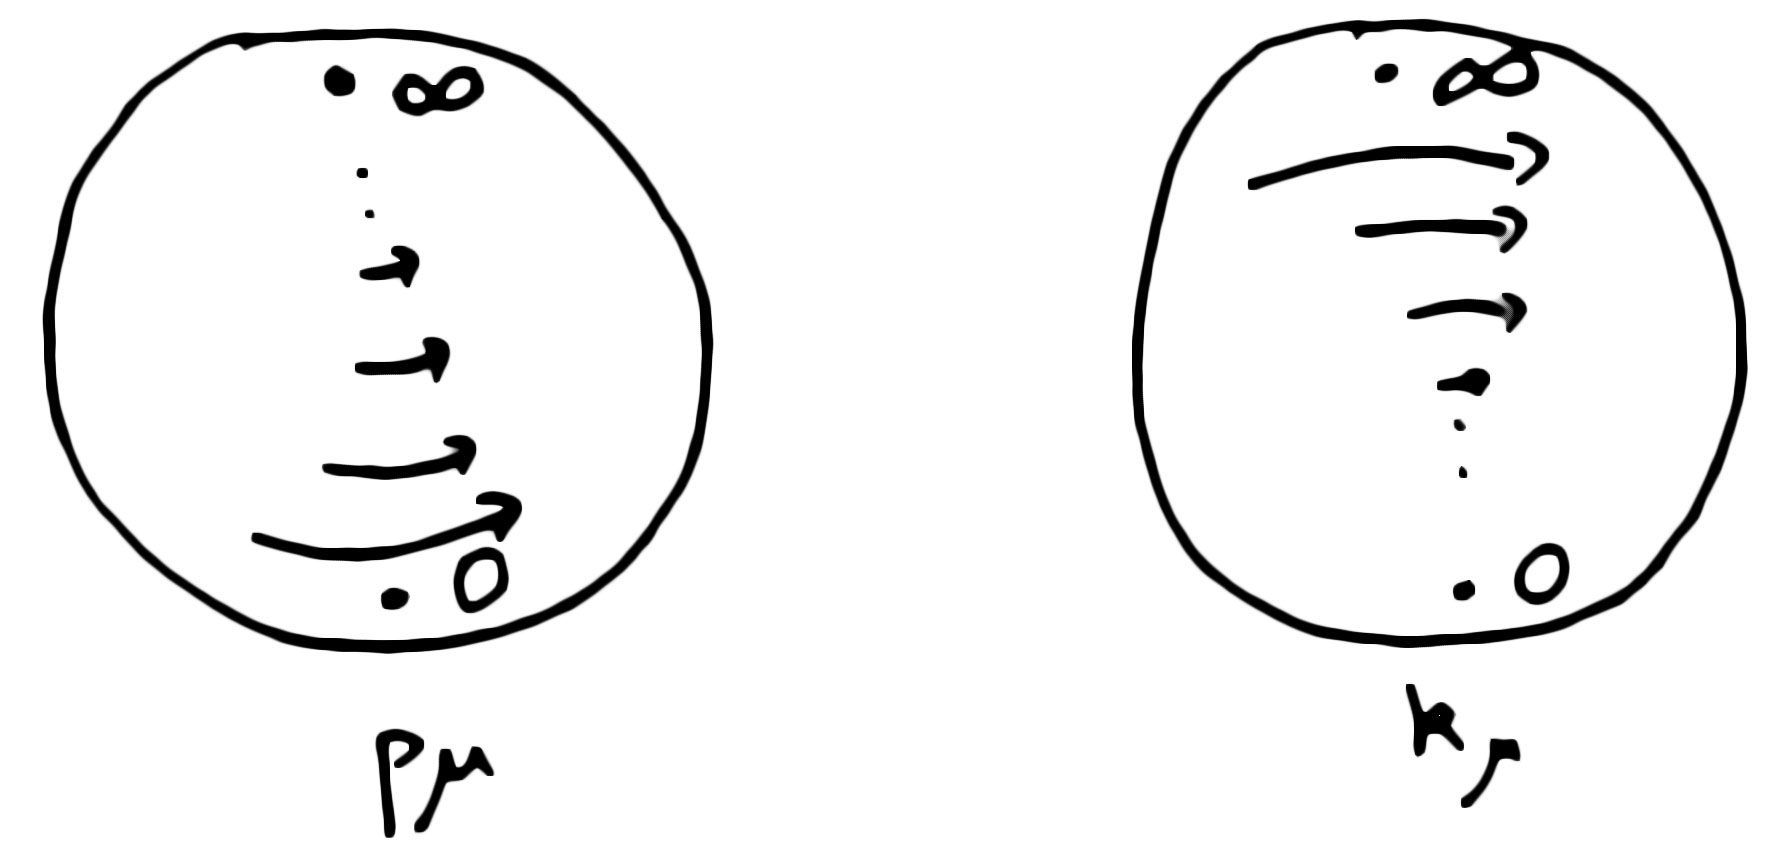
\includegraphics[width=0.5\textwidth]{translationnearinfinity.jpg}
\end{center}
\caption{\label{fig:translationnearinfinity} $k_\mu$ is analogous to $p_\mu$, with the origin and the point at infinity swapped by an inversion.}
\end{figure}

\subsection{The conformal algebra}

The charges $Q_\e$ give a representation of the conformal algebra
\be
\label{eq:conformalalgebra}
[Q_{\e_1},Q_{\e_2}] &= Q_{-[\e_1,\e_2]},
\ee
where $[\e_1,\e_2]$ is a commutator of vector fields.\footnote{The minus sign in (\ref{eq:conformalalgebra}) comes from the fact that when charges $Q_i$ are represented by differential operators $\cD_i$, repeated action reverses the order $[Q_1,[Q_2,\cO]]=\cD_2 \cD_1 \cO$.  Alternatively, we could have introduced an extra minus sign in the $Q$'s so that $[Q,\cO]=-\cD$ and then $Q,\cD$ would have the same commutation relations.}  This is not obvious and deserves proof. In fact, it is {\it not true\/} in 2-dimensional CFTs, where the algebra of charges is a central extension of the the algebra of conformal killing vectors.

\begin{exercise}
\label{exercise:primarytransofmationfort}
Show that in $d\geq 3$,
\be
\label{eq:conformaltransfofT}
[Q_\e,T^{\mu\nu}] &= \e^\rho\ptl_\rho T^{\mu\nu}+(\ptl\.\e)T^{\mu\nu}-\ptl_\rho \e^\mu T^{\rho\nu}+\ptl^\nu\e_\rho T^{\rho\mu}.
\ee
Argue as follows. Assume that only the stress tensor appears on the right-hand side.\footnote{Bonus exercise: can other operators appear?} Using linearity in $\e$, dimensional analysis, and the conformal Killing equation, show that (\ref{eq:conformaltransfofT}) contains all terms that could possibly appear.\footnote{The terms on the right-hand side are local in $\e$ because we can evaluate $[Q_{\e},T^{\mu\nu}(x)]$ in an arbitrarily small neighborhood of $x$. Assuming the singularity as two $T^{\mu\nu}$'s coincide is bounded, we can then replace $\e$ by its Taylor expansion around $x$.}  Fix the relative coefficients using conservation, tracelessness, and symmetry under $\mu\leftrightarrow \nu$. Fix the overall coefficient by matching with (\ref{commutator}).
\end{exercise}

\begin{exercise}
Using (\ref{eq:conformaltransfofT}), prove the commutation relation (\ref{eq:conformalalgebra}).
\end{exercise}

\begin{exercise}
\label{exercise:virasoro}
When $d=2$, it's possible to add two extra terms in (\ref{eq:conformaltransfofT}) proportional to the unit operator that are consistent with dimensional analysis, conservation, and tracelessness.  One of these terms breaks parity ($i.e.$ it depends on the 2d epsilon symbol) and the other doesn't. Find the parity-preserving term (up to an overall coefficient),\footnote{The coefficient can be fixed by studying a two-point function of stress tensors, see section~\ref{sec:determinec}. It is proportional to the central charge $c$.} and show how it modifies the commutation relations (\ref{eq:conformalalgebra}). This is the Virasoro algebra! Bonus question: what is the parity-breaking term?
\end{exercise}

\draftnote{Write out more of this in detail.}

As usual, (\ref{eq:conformalalgebra}) is true in any quantization of the theory.  In path integral language, it tells us how to move the topological surface operators $Q_{\e}(\Sigma)$ through each other.

\begin{exercise} Show that
\be
\,[M_{\mu\nu},P_\rho] &= \de_{\nu\rho}P_\mu - \de_{\mu\rho}P_\nu,\\
\,[M_{\mu\nu},K_\rho] &= \de_{\nu\rho}K_\mu - \de_{\mu\rho}K_\nu,\\
\,[M_{\mu\nu},M_{\rho\s}] &= \de_{\nu\rho}M_{\mu\s}-\de_{\mu\rho}M_{\nu\s}+\de_{\nu\s}M_{\rho\mu}-\de_{\mu\s}M_{\rho\nu},\label{eq:mmcommutator}\\
\label{eq:dpcommutator}
\,[D,P_\mu]&=P_\mu,\\
\label{eq:dkcommutator}
\,[D,K_\mu]&=-K_\mu,\\
\,[K_\mu,P_\nu]&=2\de_{\mu\nu}D-2M_{\mu\nu},
\ee
and all other commutators vanish.
\end{exercise}
The first three commutation relations say that $M_{\mu\nu}$ generates the algebra of Euclidean rotations $\SO(d)$ and that $P_\mu,K_\mu$ transform as vectors.  The last three are more interesting.  Equations~(\ref{eq:dpcommutator}) and (\ref{eq:dkcommutator}) say that $P_\mu$ and $K_\mu$ can be thought of as raising and lowering operators for $D$. We will return to this idea shortly.

\begin{exercise} Define the generators
\label{eq:conformalgeneratorssodplus}
\be
\label{eq:conformalgeneratorssodplus11}
L_{\mu\nu}&=M_{\mu\nu},\nn\\
L_{-1,0} &= D,\nn\\
L_{0,\mu} &= \frac 1 2 (P_\mu+K_\mu),\nn\\
L_{-1,\mu}&= \frac 1 2 (P_\mu-K_\mu),
\ee
where $L_{ab}=-L_{ba}$ and $a,b\in \{-1,0,1,\dots,d\}$. Show that $L_{ab}$ satisfy the commutation relations of $\SO(d+1,1)$. The metric in $d{+}2$-dimensions is diagonal with $g_{-1,-1}=-1$, and $g_{ii}=+1$ for $i=0,\dots,d$. 
\end{exercise}
The fact that the conformal algebra is $\SO(d+1,1)$ suggests that it might be good to think about its action in terms of $\R^{d+1,1}$ instead of $\R^d$.  This is the idea behind the ``embedding space formalism" \cite{Dirac:1936fq,Mack:1969rr,Boulware:1970ty,Ferrara:1973eg,Weinberg:2010fx,Costa:2011mg}, which provides a simple and powerful way to understand the constraints of conformal invariance. We will be more pedestrian in this course, but I recommend reading about the embedding space formalism in the lecture notes by Penedones \cite{Joao} or Rychkov \cite{Rychkov:2016iqz}.

\stoplecture

\section{Primaries and descendants}

Now that we have our conserved charges, we can classify operators into representations of those charges.  We do this in steps. First we classify operators into Poincare representations, then scale+Poincare representations, and finally conformal representations.

\subsection{Poincare representations}

In a rotationally-invariant QFT, local operators at the origin transform in irreducible representations of the rotation group $\SO(d)$,
\be
\label{eq:rotationatorigin}
[M_{\mu\nu},\cO^a(0)]&= (\cS_{\mu\nu}){}_b{}^a\cO^b(0),
\ee
where $\cS_{\mu\nu}$ are matrices satisfying the same algebra as $M_{\mu\nu}$, and $a,b$ are indices for the $\SO(d)$ representation of $\cO$.\footnote{The funny index contractions in (\ref{eq:rotationatorigin}) ensure that $M_{\mu\nu}$ and $\cS_{\mu\nu}$ have the same commutation relations (exercise!).}\footnote{Because our commutation relations (\ref{eq:mmcommutator}) for $\SO(d)$ differ from the usual conventions by a factor of $i$, the generators $\cS_{\mu\nu}$ will be {\it anti-}hermitian, $\cS^\dag=-\cS$.}  We often suppress spin indices and write the right-hand side as simply $\cS_{\mu\nu}\cO(0)$. The action (\ref{eq:rotationatorigin}), together with the commutation relations of the Poincare group, determines how rotations act away from the origin.

\begin{figure}
\begin{center}
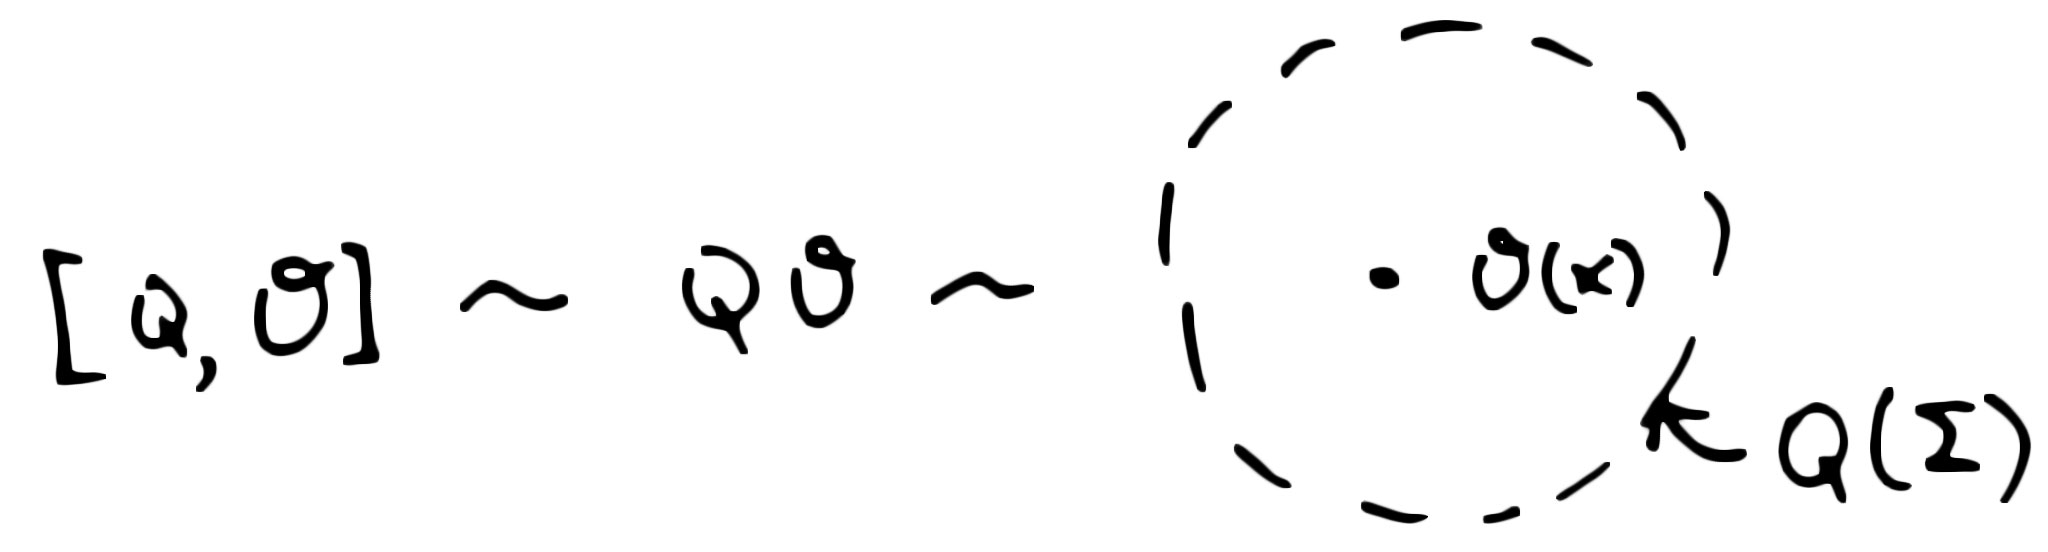
\includegraphics[width=0.5\textwidth]{commutatorissurround.jpg}
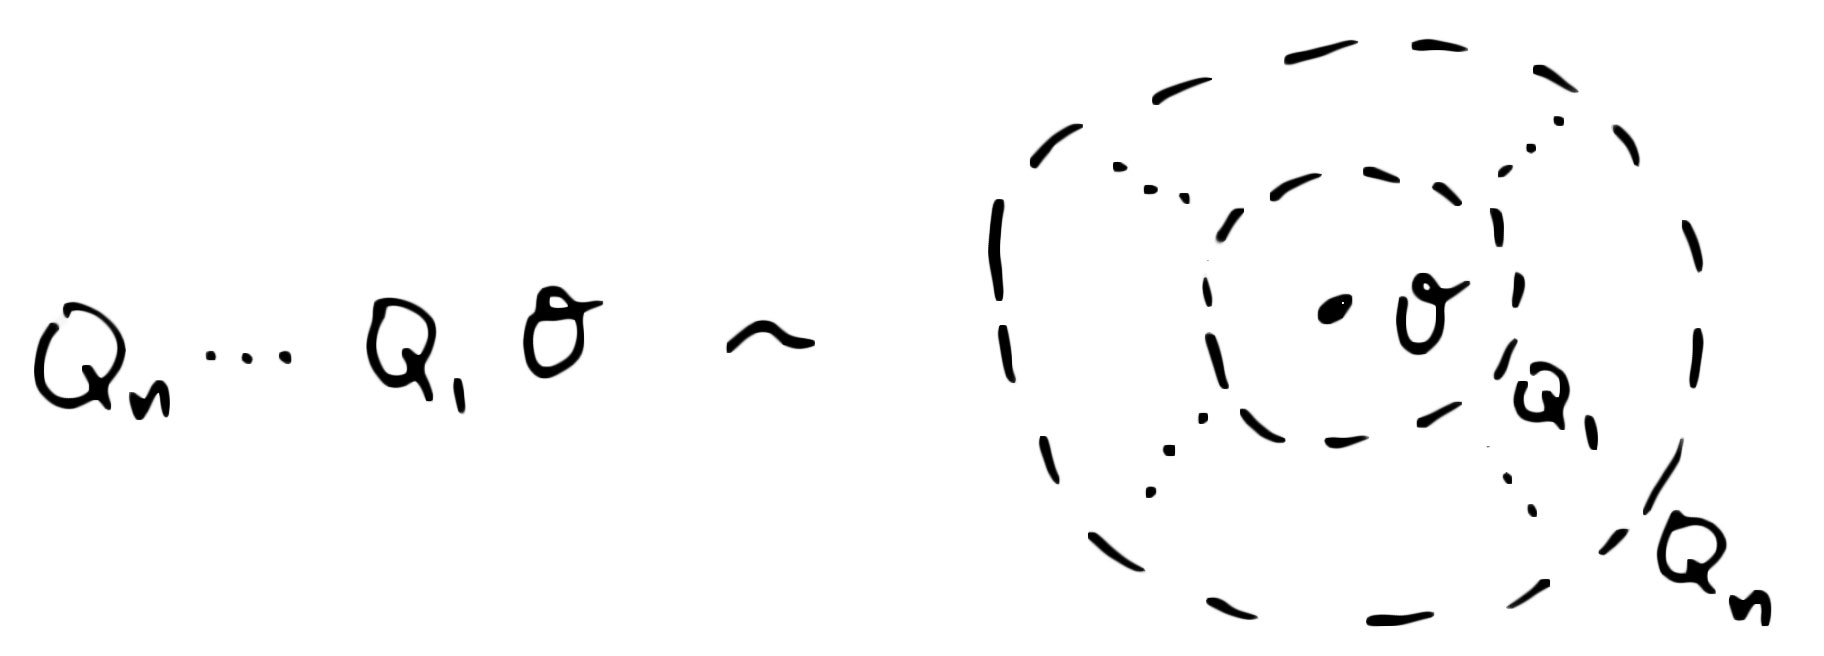
\includegraphics[width=0.5\textwidth]{surroundmany.jpg}
\end{center}
\caption{The shorthand notation $Q\cO$ stands for surrounding $\cO$ with a surface operator $Q(\Sigma)$. Equivalently, it stands for $[Q,\cO]$ in any quantization of the theory. \label{fig:commutatorissurround}}
\end{figure}

To see this, it is convenient to adopt shorthand notation where commutators of charges with local operators are implicit, $[Q,\cO] \to Q \cO$, see figure~\ref{fig:commutatorissurround}.  This notation is valid because of the Jacobi identity (more formally, the fact that adjoint action gives a representation of a Lie algebra).  In path integral language, $Q_n\cdots Q_1 \cO(x)$ means surrounding $\cO(x)$ with topological surface operators where $Q_n$ is the outermost surface and $Q_1$ is the innermost.  The conformal commutation relations tell us how to re-order these surfaces.

Acting with a rotation on $\cO(x)$, we have
\be
M_{\mu\nu}\cO(x) &= M_{\mu\nu}e^{x\.P}\cO(0) \nn\\
&= e^{x\.P}(e^{-x\.P} M_{\mu\nu} e^{x\.P})\cO(0)\nn\\
&= e^{x\.P}(-x_\mu P_\nu + x_\nu P_\mu+M_{\mu\nu})\cO(0)\nn\\
&= (x_\nu \ptl_\mu - x_\mu\ptl_\nu+\cS_{\mu\nu})e^{x\.P}\cO(0)\nn\\
&= (m_{\mu\nu}+\cS_{\mu\nu})\cO(x).\label{eq:actionbyrotation}
\ee
In the third line, we've used the Poincare algebra and the Hausdorff formula
\be
e^{A}Be^{-A} = e^{[A,\.]}B
= B+[A,B]+\frac 1 {2!}[A,[A,B]]+\dots.
\ee

\subsection{Scale+Poincare representations}

In a scale-invariant theory, it's also natural to diagonalize the dilatation operator acting on operators at the origin,
\be
\label{eq:dilatationcondition}
[D,\cO(0)]&=\Delta \cO(0).
\ee
The eigenvalue $\Delta$ is the {\it dimension\/} of $\cO$.
\begin{exercise}
Mimic the computation (\ref{eq:actionbyrotation}) to derive the action of dilatation on $\cO(x)$ away from the origin,
\be
\label{eq:dilatationaction}
[D,\cO(x)] &= (x^\mu\ptl_\mu + \Delta)\cO(x).
\ee
\end{exercise}

Equation (\ref{eq:dilatationaction}) is constraining enough to fix two-point functions of scalars up to a constant.  Firstly, by rotation and translation invariance, we must have
\be
\<\cO_1(x)\cO_2(y)\>&=f(|x-y|),
\ee
for some function $f$.

In a scale-invariant theory with scale-invariant boundary conditions, the simultaneous action of $D$ on all operators in a correlator must vanish, as illustrated in figure~\ref{fig:wardidentityford}.  Moving $D$ to the boundary gives zero.\footnote{It is also interesting to consider non-scale-invariant boundary conditions. These can be interpreted as having a nontrivial operator at $\oo$.}  On the other hand, shrinking $D$ to the interior gives the sum of its actions on the individual operators.  By the Ward identity (\ref{eq:dilatationaction}), this is
\be
\label{eq:wardidentityforcorrelator}
0 &= \p{x^\mu\ptl_\mu + \Delta_1+y^\mu\ptl_\mu+\Delta_2}f(|x-y|).
\ee
We could alternatively derive (\ref{eq:wardidentityforcorrelator}) by working in some quantization, where it follows from trivial algebra and the fact that $D|0\> = 0$,
\be
0 &= \<0|[D,\cO_1(x)\cO_2(y)]|0\>\nn\\
&= \<0|[D,\cO_1(x)]\cO_2(y)+\cO_1(x)[D,\cO_2(y)]|0\>\nn\\
&= \p{x^\mu\ptl_\mu + \Delta_1+y^\mu\ptl_\mu+\Delta_2}\<0|\cO_1(x)\cO_2(y)|0\>.
\ee
Either way, the solution is
\be
f(|x-y|) &= \frac{C}{|x-y|^{\Delta_1+\Delta_2}}.
\ee


If we had an operator with negative scaling dimension, then its correlators would grow with distance, violating cluster decomposition. This is unphysical, so we expect dimensions $\De$ to be positive. Shortly, we will prove this fact for unitary conformal theories (and derive even stronger constraints on $\De$).

\begin{figure}
\begin{center}
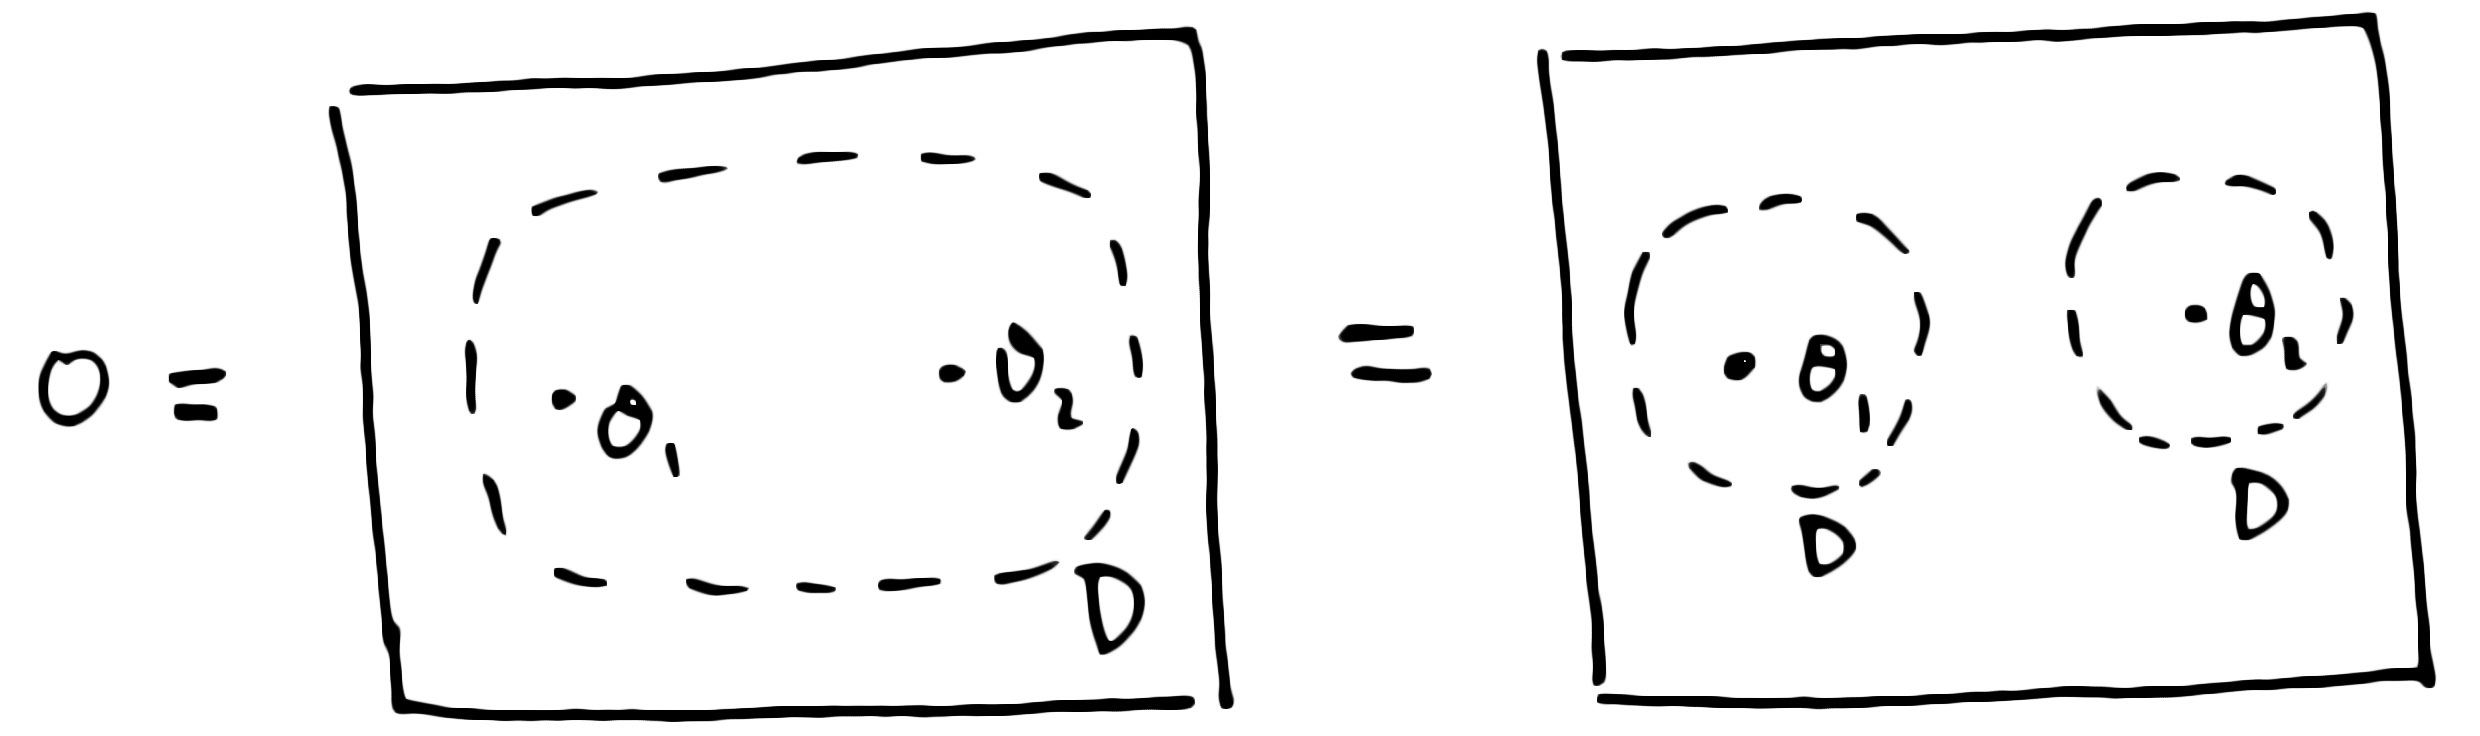
\includegraphics[width=0.75\textwidth]{wardidentityford.jpg}
\end{center}
\caption{The Ward identity for scale invariance of a two-point function. \label{fig:wardidentityford}}
\end{figure}


\subsection{Conformal representations}
\label{sec:conformalreps}

Note that $K_\mu$ is a lowering operator for dimension,
\be
D K_\mu \cO(0) &= ([D,K_\mu] + K_\mu D)\cO(0)\nn\\
&= (\De-1)K_\mu \cO(0).
\ee
(Again, we're using shorthand notation $[Q,\cO]\to Q\cO$.)  Thus, given an operator $\cO(0)$, we can repeatedly act with $K_\mu$ to obtain operators $K_{\mu_1}\dots K_{\mu_n}\cO(0)$ with arbitrarily low dimension.  Because dimensions are bounded from below in physically sensible theories, this process must eventually terminate.  That is, there must exist operators such that
\be
\label{eq:primarycondition}
[K_\mu,\cO(0)] &= 0\qquad\textrm{(primary operator)}.
\ee
Such operators are called ``primary."  Given a primary, we can construct operators of higher dimension, called ``descendants," by acting with momentum generators, which act like raising operators for dimension,
\be
\cO(0) &\to P_{\mu_1}\cdots P_{\mu_n}\cO(0)\qquad\textrm{(descendant operators)}\nn\\
\De &\to \De+n.
\ee
For example, $\cO(x)=e^{x\.P}\cO(0)$ is an (infinite) linear combination of descendant operators.
The conditions (\ref{eq:rotationatorigin},~\ref{eq:dilatationcondition},~\ref{eq:primarycondition}) are enough to determine how $K_\mu$ acts on any descendant using the conformal algebra.  For example,
\begin{exercise}
Let $\cO(0)$ be a primary operator with rotation representation matrices $\cS_{\mu\nu}$ and dimension $\Delta$.  Using the conformal algebra, show
\be
[K_\mu, \cO(x)] &= (k_\mu + 2\De x_\mu - 2x^\nu \cS_{\mu\nu})\cO(x),
\label{eq:actionofK}
\ee
where $k_\mu$ is the conformal Killing vector defined in~(\ref{eq:extraconformalgenerators}). 
\end{exercise}

To summarize, a primary operator satisfies
\be
\label{eq:isotropyaction}
\,[D,\cO(0)] &= \De\cO(0)\nn\\
\,[M_{\mu\nu},\cO(0)] &= \cS_{\mu\nu}\cO(0)\nn\\
\,[K_\mu,\cO(0)] &= 0.
\ee
From these conditions, we can construct a representation of the conformal algebra out of 
$\cO(0)$ and its descendants,
\be
\label{eq:conformalrepresentation}
\begin{array}{c|c}
\textrm{operator} & \textrm{dimension}
\\
\hline
\vdots & \\
P_{\mu_1}P_{\mu_2}\cO(0) & \De+2\\
\uparrow & \\
P_{\mu_1} \cO(0) & \De+1\\
\uparrow &\\
\cO(0) & \De.
\end{array}
\ee
The action of conformal generators on each state follows from the conformal algebra.  This should remind you of the construction of irreducible representations of $\SU(2)$ starting from a highest-weight state.  In this case, our primary is a {\it lowest-weight\/} state of $D$, but the representation is built in an analogous way.\footnote{Generically, the representation (\ref{eq:conformalrepresentation}) is an {\it induced representation} $\mathrm{Ind}^G_H(R_H)$, where $H$ is the subgroup of the conformal group generated by $D,M_{\mu\nu},K_\mu$ (called the isotropy subgroup), $R_H$ is the finite-dimensional representation of $H$ defined by (\ref{eq:isotropyaction}), and $G$ is the full conformal group. It is also called a parabolic Verma module.  Sometimes the operator $\cO$ satisfies ``shortening conditions" where a linear combination of descendants vanishes. (A conserved current is an example.)  In this case, the Verma module is reducible and the actual conformal multiplet of $\cO$ is one of the irreducible components.}  It turns out that any local operator in a unitary CFT is a linear combination of primaries and descendants. We will prove this in section~\ref{sec:onlyprimariesanddescendants}.

\begin{exercise}
Show that (\ref{commutator}), (\ref{eq:actionbyrotation}), (\ref{eq:dilatationaction}), and (\ref{eq:actionofK}) can be summarized as
\be
\label{eq:generatorsummary}
[Q_\e,\cO(x)] &= \p{\e\.\ptl + \frac{\De}{d}(\ptl\.\e) - \frac 1 2 (\ptl^\mu \e^\nu)\cS_{\mu\nu}}\cO(x).
\ee
\end{exercise}

\begin{exercise}
Deduce that $T^{\mu\nu}$ is primary by comparing (\ref{eq:generatorsummary}) with (\ref{eq:conformaltransfofT}). 
\end{exercise}

\subsection{Finite conformal transformations}

An exponentiated charge $U=e^{Q_\e}$ implements a finite conformal transformation.  Denote the corresponding diffeomorphism $e^{\e}$ by $x\mapsto x'(x)$. By comparing with (\ref{eq:conformalinfinitesimal}) and (\ref{eq:conformalfinite}), we find that (\ref{eq:generatorsummary}) exponentiates to
\be
\label{eq:finiteprimarytransformation}
U \cO^a(x) U^{-1} &= \Omega(x')^\De \rho^a{}_b(R(x')^{-1})\cO^b(x'),
\ee
where as before
\be
\pdr{x'^\mu}{x^\nu} &= \Omega(x')R^\mu{}_\nu(x'),\qquad R^\mu{}_\nu(x')\in\SO(d).
\ee
Here, $\rho^a{}_b(R)$ is a matrix implementing the action of $R$ in the $\SO(d)$ representation $\rho$ of $\cO$, for example
\begin{align}
\rho(R) &= 1 & \textrm{(scalar representation)},\nn\\
\rho^\mu{}_\nu(R) &= R^\mu{}_\nu & \textrm{(vector representation)},\label{eq:vectorrep}\nn\\
 &\cdots& \cdots
\end{align}
and so on.

We could have started the whole course by taking (\ref{eq:finiteprimarytransformation}) as the definition of a primary operator. But the connection to the underlying conformal algebra will be crucial in what follows, so we have chosen to derive it.

\begin{exercise}
Show that the transformation (\ref{eq:finiteprimarytransformation}) composes correctly to give a representation of the conformal group.  That is, show
\be
U_{g_1}U_{g_2}\cO^a(x) U_{g_2}^{-1} U_{g_1}^{-1} &= U_{g_1g_2}\cO^a(x)U_{g_1g_2}^{-1}
\ee
where $x\mapsto g_{i}(x)$ are conformal transformations, $g_1g_2$ denotes composition $x\mapsto g_1(g_2(x))$, and $U_{g}$ is the unitary operator associated to $g$.
\end{exercise}

\stoplecture

\section{Conformal correlators}

\subsection{Scalar operators}
\label{sec:conformalcorrelatorsscalars}

We have already seen that scale invariance fixes two-point functions of scalars up to a constant
\be
\label{eq:scaletwoptfunction}
\<\cO_1(x_1)\cO_2(x_2)\> &= \frac{C}{|x_1-x_2|^{\De_1+\De_2}} \qquad\textrm{(SFT)}.
\ee

For primary scalars in a CFT, the correlators must satisfy a stronger Ward identity,
\be
\label{eq:scalarconformalcorrelator}
\<\cO_1(x_1)\dots\cO_n(x_n)\> &= \<(U\cO_1(x_1)U^{-1}) \cdots (U\cO_n(x_n)U^{-1})\>\nn\\
 &= \Omega(x_1')^{\De_1}\cdots\Omega(x_n')^{\De_n}\<\cO_1(x_n')\cdots \cO_n(x_n')\>.
\ee
Let us check whether this holds for (\ref{eq:scaletwoptfunction}).

\begin{exercise}
Show that for a conformal transformation,
\be
\label{eq:conformaltransformationofdistance}
(x-y)^2 &= \frac{(x'-y')^2}{\Omega(x')\Omega(y')}.
\ee
Hint: This is obviously true for translations, rotations, and scale transformations. It suffices to check it for inversions $I:x\to\frac{x}{x^2}$ (why?).
\end{exercise}
Using (\ref{eq:conformaltransformationofdistance}), we find
\be
\frac{C}{|x_1-x_2|^{\De_1+\De_2}} &= \Omega(x_1')^{\frac{\De_1+\De_2}{2}}\Omega(x_2')^{\frac{\De_1+\De_2}{2}}\frac{C}{|x_1'-x_2'|^{\De_1+\De_2}}.
\ee
Consistency with (\ref{eq:scalarconformalcorrelator}) then requires $\De_1=\De_2$ or $C=0$.  In other words,
\be
\<\cO_1(x_1)\cO_2(x_2)\> &= \frac{C\de_{\De_1\De_2}}{x_{12}^{2\De_1}}\qquad\textrm{(CFT, primary scalars)},
\ee
where $x_{12}\equiv x_1-x_2$.
\begin{exercise}
Recover the same result using the Ward identity for $K_\mu$
\be
\<[K_\mu,\cO_1(x_1)]\cO_2(x_2)\>+\<\cO_1(x_1)[K_\mu,\cO_2(x_2)]\> &= 0.
\ee
\end{exercise}

Conformal invariance is also powerful enough to fix a three-point function of primary scalars, up to an overall coefficient.  Using (\ref{eq:conformaltransformationofdistance}), it's easy to check that the famous formula \cite{Polyakov:1970xd}
\be
\label{eq:conformalthreeptfunction}
\<\cO_1(x_1)\cO_2(x_2)\cO_3(x_3)\> &= \frac{f_{123}}{x_{12}^{\De_1+\De_2-\De_3}x_{23}^{\De_2+\De_3-\De_1}x_{31}^{\De_3+\De_1-\De_2}},
\ee
with $f_{123}$ constant, satisfies the Ward identity (\ref{eq:scalarconformalcorrelator}). Here, we use the notation $x_{ij}\equiv x_i-x_j$ and $x^a=(x^2)^{a/2}$.

With four points, there are nontrivial conformally invariant combinations of the points called ``conformal cross-ratios,"
\be
\label{eq:definitionofcrossratios}
u = \frac{x_{12}^2 x_{34}^2}{x_{13}^2 x_{24}^2},\qquad
v = \frac{x_{23}^2 x_{14}^2}{x_{13}^2 x_{24}^2}.
\ee
The reason that there are exactly two independent cross-ratios can be understood as follows.
\begin{itemize}
\item Using special conformal transformations, we can move $x_4$ to infinity.
\item Using translations, we can move $x_1$ to zero.
\item Using rotations and dilatations, we can move $x_3$ to $(1,0,\dots,0)$.
\item Using rotations that fix $x_3$, we can move $x_2$ to $(x,y,0,\dots,0)$.
\end{itemize}

\begin{figure}
\begin{center}
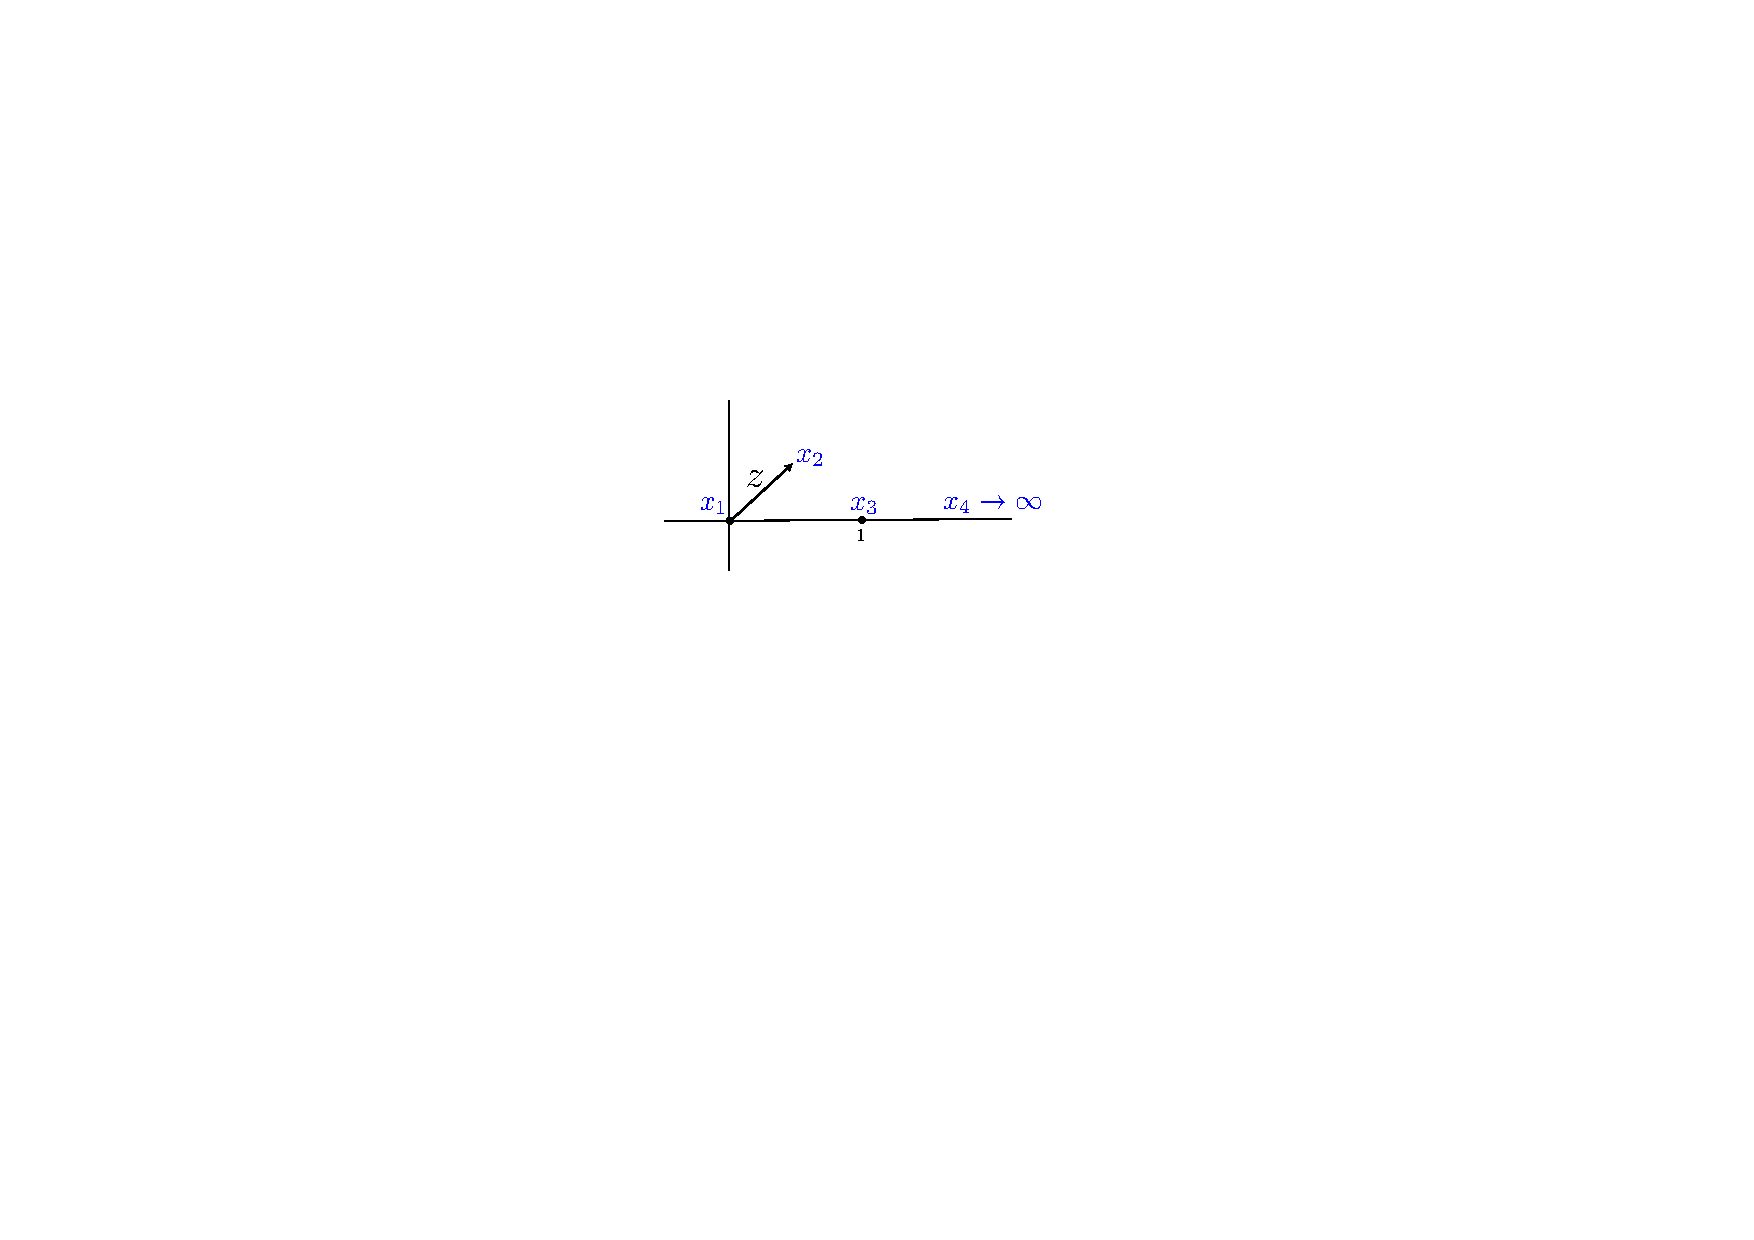
\includegraphics[width=0.4\textwidth]{fig-z}
\end{center}
\caption{\label{fig:zplane} Using conformal transformations, we can place four points on a plane in the configuration shown above (figure from \cite{Hogervorst:2013sma}).}
\end{figure}

This procedure leaves exactly two undetermined quantities $x,y$, giving two independent conformal invariants. Evaluating $u$ and $v$ for this special configuration of points (figure~\ref{fig:zplane}) gives
\be
u=z\bar z,\qquad v=(1-z)(1-\bar z),
\ee
where $z\equiv x+iy$.

Four-point functions can depend nontrivially on the cross-ratios.  For a scalar $\f$ with dimension $\De_\phi$, the formula
\be
\label{eq:fourptfunctionofprimaries}
\<\f(x_1)\f(x_2)\f(x_3)\f(x_4)\> &= \frac{g(u,v)}{x_{12}^{2\De_\f}x_{34}^{2\De_\f}}
\ee
satisfies the Ward identity (\ref{eq:scalarconformalcorrelator}) for any function $g(u,v)$. 
\begin{exercise}
Generalize (\ref{eq:fourptfunctionofprimaries}) to the case of non-identical scalars $\f_i(x)$ with dimensions $\De_i$.
\end{exercise}

The left-hand side of (\ref{eq:fourptfunctionofprimaries}) is manifestly invariant under permutations of the points $x_i$.  This leads to consistency conditions on $g(u,v)$,
\begin{align}
\label{eq:trivialcrossing}
g(u,v) &= g(u/v,1/v) & \textrm{(from swapping $1\leftrightarrow 2$ or $3\leftrightarrow 4$)},\\
\label{eq:crossingsymmetry}
g(u,v) &= \p{\frac{u}{v}}^{\De_\f} g(v,u) & \textrm{(from swapping $1\leftrightarrow 3$ or $2\leftrightarrow 4$)}.
\end{align}
All other permutations can be generated from the ones above.  We will see shortly that $g(u,v)$ is  actually determined in terms of the dimensions $\De_i$ and three-point coefficients $f_{ijk}$ of the theory.  Equation~(\ref{eq:trivialcrossing}) will be satisfied for trivial reasons.  However (\ref{eq:crossingsymmetry}) will lead to powerful constraints on the $\De_i, f_{ijk}$.

\subsection{Spinning operators: the conformal frame approach}

For operators with spin, the solutions to the conformal Ward identities are more complicated. We will discuss two different approaches, both with advantages and disadvantages. The first approach is to relate an arbitrary configuration of points to some standard configuration (``conformal frame"), where the Ward identities are easier to solve. This is the same type of argument we used above to show that a four-point function can depend on two conformal cross-ratios.

\subsubsection{Two-point functions}
\label{sec:twoptsection}

Consider a two-point function of primary operators $\cO_1^a, \cO_2^b$ transforming in representations $\rho_1,\rho_2$ of $\SO(d)$, with dimensions $\De_1,\De_2$. Here, $a,b$ are indices for $\rho_1,\rho_2$, respectively. The Ward identity (\ref{eq:finiteprimarytransformation}) implies
\be
&\<\cO_1^a(x_1) \cO_2^b(x_2)\>\nn\\
&=\<U\cO_1^a(x_1)U^{-1} U \cO_2^b(x_2) U^{-1}\>\nn\\
&= \Omega(x_1')^{\De_1} \Omega(x_2')^{\De_2}\, (\rho_1)^a{}_c(R(x_1')^{-1})\, (\rho_2)^b{}_d(R(x_2')^{-1}) \,\<\cO_1^c(x_1')\cO_2^d(x_2')\>.
\label{eq:specializedtwoptward}
\ee
Using translations, we have
\be
\<\cO_1^a(x_1) \cO_2^b(x_2)\> &= \<\cO_1^a(0) \cO_2^b(x_2-x_1)\>.
\ee
Using the Ward identity for rescaling, we have
\be
\label{eq:rescalingward}
\<\cO_1^a(0) \cO_2^b(x)\> &= \frac{1}{|x|^{\De_1+\De_2}} \<\cO_1^a(0) \cO_2^b(\hat x)\>,\quad\hat x \equiv \frac{x}{|x|}.
\ee
Now fix a unit vector $e$, and let $Q^{\mu}{}_\nu(\hat x)$ be any rotation that takes $e$ to $\hat x$. ($Q(\hat x)$ is not unique, but this won't matter.) Using the Ward identity for rotations, we can relate the correlator at $\hat x$ to the correlator at $e$,
\be
\label{eq:rotationward}
\<\cO_1^a(0) \cO_2^b(\hat x)\> &= (\rho_1)^a{}_c(Q(\hat x)) (\rho_2)^b{}_d(Q(\hat x))\<\cO_1^c(0) \cO_2^d(e)\>.
\ee
Thus, once we know the two-point function for the points $0,e$, we know it everywhere.

We cannot specialize the points any further.  However, the correlator $\<\cO_1^c(0) \cO_2^d(e)\>$ satisfies more constraints because there are conformal transformations that leave the points $0,e$ invariant but act nontrivially on the correlator. The subgroup of $\SO(d+1,1)$ that leaves a set of points invariant is called the ``stabilizer group" of those points, and our claim is that the stabilizer group of two points is nontrivial.

The easiest stabilizer group to analyze is when the two points are $0,\oo$. In this case, we can apply any rotation and dilatation, so the stabilizer group is $\R^+\x \SO(d)$. It's useful to imagine $0,\oo$ as the south and north pole of the sphere via stereographic projection. From this point of view, it's clear that dilatations and rotations act in different ways near each point. A dilatation $x\mapsto\l x$ with $\l>1$ moves points away from 0 and towards $\oo$. A rotation around the origin gets reflected near $\oo$.

To construct the stabilizer group of $0,e$, we can conjugate the stabilizer group of $0,\oo$ by a transformation that maps between the two configurations. In particular, the stabilizer group of any pair of points is $\R^+\x\SO(d)$. Consider an inversion $I:x\mapsto \frac{x}{x^2}$. This fixes $e$, but moves the origin to $\oo$. Now, we can perform an arbitrary rescaling and rotation around $e$ without moving either $e$ or $\oo$:
\be
x^\mu &\mapsto e^\mu + \l^{-1} h^\mu{}_\nu (x - e)^\nu,\qquad \l\in\R^+,\ h\in \SO(d).
\ee
Finally, we can invert again to map infinity back to the origin. Overall, we have constructed
\be
\label{eq:mapdefinition}
x\mapsto x'(x) = I(e + \l^{-1} h(I(x) - e)),\qquad I(x) = \frac{x}{x^2},
\ee
parameterized by $\l,h$. Note that because we used $I$ twice, this map is in the connected component of the identity of $\SO(d+1,1)$, and is thus always a symmetry in a CFT. %We have found that the stabilizer group of two points is $\R^+ \x \SO(d) \subset \SO(d+1,1)$.

Let us study the behavior of (\ref{eq:mapdefinition}) near the fixed-points $0,e$. An important object will be the derivative of an inversion
\be
\pdr{I(x)^\mu}{x^\nu} &= \frac 1 {x^2}\p{\de^\mu_\nu - \frac{2x^\mu x_\nu}{x^2}} \equiv \frac{1}{x^2} I^\mu{}_\nu(x).
\ee
Here we have expressed it as an overall rescaling factor $\frac{1}{x^2}$, times an orthogonal matrix $I^\mu{}_\nu(x)$ that represents a reflection in the $x$ direction.\footnote{It is not an element of $\SO(d)$ because $i$ is not an element of $\SO(d+1,1)$. Instead, $i\in O(d+1,1)$ and consequently $I(x)\in O(d)$.}
Near the point $e$, the map $x'(x)$ first reflects in the $e$ direction, then rescales and rotates, then reflects back. Thus, we have
\be
x'(x) &\sim e^\mu + \l^{-1} (I_ehI_e)^\mu{}_\nu (x-e)^\nu + O((x-e)^2),
\ee
where we're using the shorthand notation $(I_e)^\mu{}_\nu=I^\mu{}_\nu(e)$.
This looks locally like a rescaling by $\l^{-1}$ and a rotation by $\tl h = I_ehI_e^{-1}$ (note that $I_e=I_e^{-1}$ because it is a reflection).
Near the point $0$, we have
\be
x'(x) &\sim \l h^\mu{}_\nu x^\nu + O(x^2),
\ee
which looks locally like a rescaling by $\l$ and a rotation by $h$. This is consistent with what we saw on the sphere: dilatations move between the two fixed points, and rotations get reflected when we go from one fixed-point to another.

The Ward identity (\ref{eq:specializedtwoptward}) implies
\be
\label{eq:fancytwoptWardidentity}
\<\cO_1^a(0) \cO_2^b(e)\> &= \l^{\De_1-\De_2} (\rho_1)^a{}_c(h^{-1}) (\rho_2)^b{}_d(\tl h^{-1}) \<\cO_1^c(0) \cO_2^d(0)\>.
\ee
This must hold for all $\l$, which immediately means $\De_1=\De_2$, as we concluded before.

To understand the $h$-dependent part, consider vector operators,
\be
\<V_1^\mu(0) V_2^\nu(e)\>\equiv Y^{\mu\nu}.
\ee
Our Ward identity says (replacing $h\to h^{-1}$ for simplicity),
\be
h^\mu{}_\rho (I_e h I_e)^\nu{}_\s Y^{\rho \s} &= Y^{\rho \s},
\ee
or in matrix notation
\be
h Y I_e h^T I_e = Y\quad \implies \quad h (YI_e) h^T = (YI_e).
\ee
In other words, $YI_e$ must be invariant under conjugation by an arbitrary $\SO(d)$ transformation, which means $Y\propto I_e$. Thus we have
\be
\<V_1^\mu(0) V_2^\nu(e)\> &= c_{12} I^{\mu\nu}(e) = c_{12}(\de^{\mu\nu} - 2e^\mu e^\nu),
\ee
for some constant $c_{12}$.
Applying (\ref{eq:rescalingward}) and (\ref{eq:rotationward}),\footnote{Note that the exact definition of $Q(\hat x)$ doesn't matter, since we only needed $Q(\hat x)e=\hat x$.}
\be
\label{eq:finalresultforVV}
\<V_1^\mu(0) V_2^\nu(x)\> &= c_{12}\frac{I^{\mu\nu}(x)}{x^{2\De}} = c_{12}\frac{\de^{\mu\nu}-\frac{2x^\mu x^\nu}{x^2}}{x^{2\De}}.
\ee
Note that conformal invariance fixes the relative factor between $\de^{\mu\nu}$ and $\frac{x^\mu x^\nu}{x^2}$ (which is not possible with scale invariance alone).\footnote{One can give a much simpler derivation of (\ref{eq:finalresultforVV}) by anticipating the fact that it is actually invariant under an inversion $I$, and not just elements of $\SO(d+1,1)$.  However, $I$ is only guaranteed to be a symmetry in parity-invariant theories (exercise~\ref{}). The derivation here assumes only $\SO(d+1,1)$-invariance.}

Here, we see why the choice of $Q(\hat x)$ doesn't matter: the correlator $\<V_1(0)V_2(e)\>$ is invariant under rotations that fix $e$ (this is a subgroup of the stabilizer group $\SO(d-1)\subset \R^+\x \SO(d)$), and two different $Q(\hat x)$'s will differ by an $\SO(d-1)$ rotation. More concretely, $\<V_1(0)V_2(e)\>$ depends only on $\de^{\mu\nu}$ and $e^\mu$, so the effect of $Q(\hat x)$ is just to replace $e\to \hat x$.

\stoplecture

For traceless symmetric tensor operators $\cO_1^{\mu_1\cdots\mu_\ell}$ and $\cO_2^{\mu_1\cdots\mu_{\ell'}}$, the two-point function can only be nonvanishing if the spins are equal $\ell=\ell'$. In that case, the two-point function takes the form
\be
\label{eq:symmetrictensortwopt}
\<\cO_1^{\mu_1\cdots\mu_\ell}(0) \cO_{2,\nu_1\cdots\nu_\ell}(x)\> &= c_{12}\frac{I^{(\mu_1}{}_{(\nu_1}(x) \cdots I^{\mu_\ell)}{}_{\nu_\ell)}(x) - \textrm{traces}}{x^{2\De}}.
\ee
Here, parentheses $(\mu_1\cdots\mu_\ell)$ mean we symmetrize the given indices,\footnote{it is only necessary to symmetrize in either $\mu$ or $\nu$, but we symmetrize both for clarity} and ``$-\textrm{traces}$" means we subtract terms proportional to $\de^{\mu_i\mu_j}$ and $\de_{\nu_i\nu_j}$ to make the result traceless. For example, for spin-2 operators,
\be
\label{eq:spintwotwopt}
&\<\cO_1^{\mu_1\mu_2}(0) \cO_{2,\nu_1\nu_2}(x)\>\nn\\
&=
c_{12} \frac{\frac{1}{2}(I^{\mu_1}{}_{\nu_1}(x)I^{\mu_2}{}_{\nu_2}(x) + I^{\mu_2}{}_{\nu_1}(x)I^{\mu_1}{}_{\nu_2}(x)) - \frac{1}{d} \de^{\mu_1\mu_2} \de_{\nu_1\nu_2}}{x^{2\De}}.
\ee
One way to think about (\ref{eq:symmetrictensortwopt}) is that once we've identified a conformally-invariant two-point function for vectors (\ref{eq:finalresultforVV}), we can take tensor products of it (symmetrized in the appropriate way) to get conformally-invariant two-point functions for other operators.

Here is a more formal way to understand the rotation part of the Ward identity (\ref{eq:fancytwoptWardidentity}). Given a representation $\rho$ of $\SO(d)$, let us define the reflected representation $\rho^R$ by
\be
\label{eq:reflectedrep}
\rho^R(h) &\equiv \rho(I_ehI_e^{-1}),\qquad h\in \SO(d).
\ee
Note that $I_e h I_e^{-1}\in \SO(d)$, even though $I_e$ is not in $\SO(d)$ (it is a reflection). Thus, the definition (\ref{eq:reflectedrep}) makes sense.
Note also that a different choice of $e$ would lead to an equivalent representation because $I_{e'}=kI_e$ for $k\in \SO(d)$, so
\be
\rho(I_{e'}hI_{e'}^{-1}) = \rho(k)\rho(I_ehI_e^{-1}) \rho(k)^{-1}.
\ee
If two representations differ by conjugation by a matrix (in this case $\rho(k)$), they are equivalent.\footnote{The definition (\ref{eq:reflectedrep}) is an example of how the outer automorphisms $\mathrm{Out}(G)$ of a group $G$ act on the ring of $G$-representations. Here, conjugation by $I_e$ is an outer automorphism of $\SO(d)$.}

\begin{exercise}
\label{eq:reflectedreps}
Show that in four dimensions, the reflection of a left-handed spinor $\psi_\a$ is a right-handed spinor $\bar\psi_{\dot\a}$, and the reflection of a self-dual two-form $F_{\a\b}$ is an anti-self-dual two-form $F_{\dot\a\dot\b}$.
\end{exercise}

The Ward identity (\ref{eq:fancytwoptWardidentity}) can be written
\be
\<\cO_1^a(0) \cO_2^b(e)\> &= (\rho_1)^a{}_c(h) (\rho_2^R)^b{}_d(h) \<\cO_1^c(0) \cO_2^d(0)\>.
\ee
In other words, $\<\cO_1^a(0) \cO_2^b(e)\>$ is an invariant-tensor transforming in the tensor product $\rho_1 \otimes \rho_2^R$.  If $\rho_1,\rho_2$ are irreducible, then such an invariant exists only if $\rho_1 = (\rho_2^R)^*$, where ${\rho}^*$ denotes the dual of $\rho$. Furthermore, if it exists it is unique.

As an example, traceless symmetric tensors are equivalent to their dual reflected representations, so we have recovered the statement that a two-point function of spin-$\ell$ and spin-$\ell'$ operators can be nonzero only if $\ell=\ell'$. As another example, by exercise~(\ref{eq:reflectedreps}) a left-handed spinor $\psi_\a$ in 4d can only have a nonvanishing two-point function with a right-handed spinor $\bar\psi_{\dot\a}$.

\begin{exercise}
Find this two-point function of spinors in 4d. Hint:
$\<\psi_\a(0)\bar\psi_{\dot\a}(e)\>$
must have the correct indices and be invariant under rotations that fix $e$.
\end{exercise}

\subsubsection{Three-point functions}

To study a three-point function, we can use the same strategy: we use conformal transformations to fix the three points, and then study the Ward identities of the stabilizer group. For simplicity, consider the case where two of the operators $\f_1,\f_2$ are scalars and the third $\cO_3$ transforms in a nontrivial representation $\rho$ of $\SO(d)$,
\be
\<\f_1(x_1) \f_2(x_2) \cO^a_3(x_3)\>.
\ee
Now, use conformal transformations to place the three operators at $0,e,\oo$ for some fixed unit vector $e$.\footnote{As before, we would like to use inversion an even number of times, so that our transformation is in $\SO(d+1,1)$.}

To simplify the discussion, we can use a trick. Let us divide by the standard three-point structure (\ref{eq:conformalthreeptfunction}) for scalars with dimensions $\De_1,\De_2,\De_3$,
\be
\label{eq:omegatrick}
t^a(x_1,x_2,x_3) &\equiv \<\f_1(x_1) \f_2(x_2) \cO_3^a(x_3)\>x_{12}^{\De_1+\De_2-\De_3} x_{23}^{\De_2+\De_3-\De_1} x_{31}^{\De_3+\De_1-\De_2}.
\ee
The result $t^a(x_1,x_2,x_3)$ will behave like a three-point function of dimension-0 operators. We are not claiming that dimension-0 operators actually exist. This is just a trick so that we don't have to worry about $\Omega(x)$ factors when we use the Ward identities.

Let us send $x_3\mapsto\oo$ with an inversion, then translate $x_2$ to the origin and invert again to send $x_2\mapsto \oo$ and $x_3\mapsto 0$. Finally, we rescale so that $x_1$ gets mapped to a unit vector. Overall, we have
\be
x'^\mu(x) &= \frac{I(I(x-x_3)-I(x_2-x_3))^\mu}{|I(I(x_1-x_3)-I(x_2-x_3))|}.
\ee
Near the point $x_3$, this is proportional to $I(I(x-x_3))=x-x_3$, so $R(x_3')^{\mu}{}_\nu$ is trivial for this transformation (which is why we chose it). Because of our trick (\ref{eq:omegatrick}), we don't need to keep track of rescaling factors. Thus, we have
\be
t^a(x_1,x_2,x_3) &= t^a(x'(x_1),\oo,0) = t^a\p{\hat Z_3,\oo,0}, \nn\\
Z_3 &\equiv \frac{x_{13}}{x_{13}^2} - \frac{x_{23}}{x_{23}^2},\qquad \hat Z_3 = \frac{Z_3}{|Z_3|}.
\label{eq:defofz3}
\ee
Finally, let us use an orthogonal transformation $Q(\hat Z_3)$ to relate this to a standard configuration\footnote{In the case where all three operators are scalars, this verifies that there are no other solutions to the conformal Ward identities besides (\ref{eq:conformalthreeptfunction}), since $t(x_1,x_2,x_3)=t(e,\oo,0)$ is just a constant.}
\be
\label{eq:relatetostandard}
t^a(x_1,x_2,x_3) &= \rho^a{}_b(Q(\hat Z_3)) t^b(e,\oo,0).
\ee



We have fixed the three points using the conformal group. As before, the correlator is still constrained because the stabilizer group of the three points is nontrivial. It consists of $\SO(d-1)$ rotations that fix the line passing through $0,e,\oo$. The Ward identities say that
\be
t^a(e,\oo,0) &= \rho^a{}_b(h) t^b(e,\oo,0),\qquad h\in \SO(d-1).
\ee
which means that $t^a$ must live in the $\SO(d-1)$-invariant subspace of $\rho$.

As an example, consider a vector operator $V^\mu$. In this case, $t^\mu(e,\oo,0)$ carries a single vector index and must be invariant under rotations that fix $e$. The only possibility is
\be
t^\mu(e,\oo,0) = f_{123} e^\mu,
\ee
for some constant $f_{123}$. Using (\ref{eq:relatetostandard}) and (\ref{eq:omegatrick}), we find
\be
\<\f_1(x_1)\f_2(x_2)V^\mu_3(x_3)\> &= \frac{f_{123}\hat Z_3^\mu}{x_{12}^{\De_1+\De_2-\De_3} x_{23}^{\De_2+\De_3-\De_1} x_{31}^{\De_3+\De_1-\De_2}} .
\ee
Similarly, for traceless symmetric tensor operators $\cO_3^{\mu_1\cdots\mu_\ell}$, the only possibility is
\be
t^{\mu_1\cdots\mu_\ell}(e,\oo,0) &= f_{123} (e^{\mu_1}\cdots e^{\mu_\ell} - \textrm{traces}),
\ee
which leads to
\be
\label{eq:scalarscalarspinL}
\<\f_1(x_1)\f_2(x_2)\cO^{\mu_1\cdots\mu_\ell}_3(x_3)\> &= \frac{f_{123}(\hat Z_3^{\mu_1}\cdots \hat Z_3^{\mu_\ell} - \textrm{traces})}{x_{12}^{\De_1+\De_2-\De_3} x_{23}^{\De_2+\De_3-\De_1} x_{31}^{\De_3+\De_1-\De_2}} .
\ee

For any other $\SO(d)$-representation $\rho$, it's not possible to find a nonvanishing $t^a$. The mathematical reason is that only traceless symmetric tensors have an $\SO(d-1)$-invariant subspace (and that subspace is one-dimensional). More prosaically, $e^\mu$ and $\de^{\mu\nu}$ are the only $\SO(d-1)$-invariant objects we can use to build $t^a(e,\oo,0)$. If we demand irreducibility, at least one term should not contain a $\de^{\mu\nu}$ (otherwise we'd have a nonzero trace). Thus, we can only build traceless symmetric tensors.

Note that $\hat Z_3^\mu$ is odd under $x_1\leftrightarrow x_2$. Consequently, if $\f_1=\f_2$ are identical operators, the correlator $\<\f_1\f_1 \cO^{\mu_1\cdots\mu_\ell}\>$ can only be nonzero if $\ell$ is even. This fact will play an important role later.

When all three operators have nontrivial $\SO(d)$ representations $\rho_1,\rho_2,\rho_3$, the solution of the  Ward identities is similar. We again use the conformal group to place all three operators on a line. (However, the relationship between the correlator at $x_1,x_2,x_3$ and the correlator on the line is more complicated because we must keep track of all three rotations.) We then study the Ward identities for the stabilizer group $\SO(d-1)$ in this ``collinear" configuration. The solution is given by the $\SO(d-1)$-invariant subspace of the tensor product of the $\rho_i$,
\be
(\rho_1\otimes \rho_2\otimes \rho_3)^{\SO(d-1)} = \otimes_{i=1}^3 \mathrm{Res}^{\SO(d)}_{\SO(d-1)} \rho_i.
\ee
(Here, $\rho^H$ denotes the $H$-invariant subspace of $\rho$, and $\mathrm{Res}^G_H\rho$ denotes the restriction of $\rho$ from a $G$-representation to an $H$-representation for $H\subseteq G$.) This means that there can be multiple three-point structures when more than one operator has spin.

For example, consider a three-point function of two vectors and a scalar $\<V_1^\mu V_2^\nu f_3\>$. In the collinear configuration, the correlator must be $\SO(d-1)$-invariant. The only possibilities are
\be
\label{eq:vvterms}
\<V_1^\mu(e) V_2^\nu(\oo) f_3(0)\> &= f_{123}^{(1)} e^\mu e^\nu + f_{123}^{(2)} \de^{\mu\nu},
\ee
where $f_{123}^{(1)},f_{123}^{(2)}$ are constants. Abstractly, we can see that there are two structures by counting
\be
(\myng{(1)} \otimes \myng{(1)} \otimes \mathbf{1})^{\SO(d-1)} &= (\mathbf{1} \oplus \myng{(1)})\otimes (\mathbf{1} \oplus \myng{(1)}) \otimes \mathbf{1} \nn\\
&= 2\mathbf{1}\oplus 2 \myng{(1)} \oplus \myng{(2)}  \oplus \myng{(1,1)},
\ee
where we've used $\mathrm{Res}^{\SO(d)}_{\SO(d-1)}\myng{(1)} = \mathbf{1} \oplus \myng{(1)}$. This calculation reveals an additional wrinkle: notice that $\myng{(1,1)}$ is the trivial representation in $d=2$, so there are actually three structures in that case. Indeed, in $d=2$ there is another term we can include in (\ref{eq:vvterms}) proportional to $\e^{\mu\nu}$.

We can compute the correlator in a general configuration using the Ward identities. Tracing everything through, we find
\be
\<V_1^\mu(x_1) V_2^\nu(x_2) f_3(x_3)\> &= \frac{a\hat Z_1^\mu \hat Z_2^\nu + b I^{\mu\nu}(x_{12})}{x_{12}^{\De_1+\De_2-\De_3} x_{23}^{\De_2+\De_3-\De_1} x_{31}^{\De_3+\De_1-\De_2}},
\ee
where $a,b$, are linear combinations of $f_{123}^{(1)},f_{123}^{(2)}$. Here $\hat Z_1,\hat Z_2$ are analogs of $\hat Z_3$ with the points permuted. This result is suggestive that we can think about building conformally-invariant correlators by putting together simple building blocks. The embedding space formalism, which we discuss next, makes this easy to do.

\subsection{The embedding space}

The action of the conformal group on $\R^d$ is nonlinear, so it takes some work to solve the conformal Ward identities. The embedding space is a way of realizing the conformal group so that it acts {\it linearly}, which makes it much simpler to solve the conformal Ward identities.

The central observation is that the conformal group is the same as $\SO(d+1,1)$ (exercise~\ref{eq:conformalgeneratorssodplus}), which acts simply by matrix multiplication on $\R^{d+1,1}$
\be
X &\mapsto g X,\qquad X\in \R^{d+1,1},\ g\in \SO(d+1,1).
\ee
We will use coordinates $X=(X^+,X^-,X^1,\dots,X^d)$ on $\R^{d+1,1}$, with metric
\be
\label{eq:embeddingmetric}
X^2 &= -X^+ X^- + \sum_{\mu=1}^d X_\mu X^\mu.
\ee
$\R^{d+1,1}$ is a $d+2$-dimensional space, and we would like our theory to live in $d$ dimensions. 
 We can remove one dimension in a conformally-invariant way by restricting to the null cone
\be
X^2 = 0\qquad (\textrm{null cone}).
\ee
The null cone is preserved by $\SO(d+1,1)$, so we have a $d+1$-dimensional space on which the conformal group acts. To finally get to $d$-dimensions, we can projectivize, i.e.\ mod out by rescalings:
\be
\textrm{projective null cone} = \frac{\{X:X^2 = 0\}}{X\sim \l X\ \ (\l\in \R)}.
\ee
\stoplecture

In the projective null cone, each null vector $X$ represents an equivalence class, and the conformal group maps one equivalence class to another. We can think of rescaling as a ``gauge redundancy." Geometrically, the projective null cone is the space of lines contained in the null cone, and the conformal group maps one line to another. 

To be more explicit, let us fix a gauge by choosing a representative for each equivalence class. One simple gauge-fixing is $X^++X^-=1$, which is equivalent to cutting the null cone with a plane, with intersection locus $S^d$. This shows that the projective null cone is topologically equivalent to $S^d$, which we should think of as $\R^d$ plus the point at infinity. $S^d$ is called the ``conformal compactification" of $\R^d$.

The most important gauge fixing for us will be $X^+=1$, which defines the ``Poincare section" of the null cone. Given a null vector $X=(X^+,X^-,X^\mu)$, we can rescale by $1/X^+$ to obtain an equivalent vector $(1,X^-/X^+,X^\mu/X^+)$ on the Poincare section. The only case in which this doesn't work is when $X^+=0$, so that $X$ is equivalent to $(0,1,0)$. This corresponds to the point at infinity.

Every null vector on the Poincare section can be written
\be
X &= (1,x^2, x^\mu),
\ee
where $x\in \R^d$ and $x^2=x_\mu x^\mu$.\footnote{Note that the limit of $(1,x^2,x^\mu)$ as $x\to \oo$ is projectively equivalent to $(0,1,0)$, which justifies the claim that we should think of $(0,1,0)$ as the point at infinity.} Now consider the action of the conformal group, $X \mapsto g X$. Note that $gX$ may not be on the Poincare section anymore, so we must rescale by $(gX)^+$ to restore our gauge choice
\be
(1,x^2,x) = X &\mapsto g X \to (gX)/(gX)^+ = (1,x'^2,x'^\mu).
\ee
Following this chain gives a nonlinear map $x\to x'$. We claim that this is exactly the usual action of the conformal group.

To see this, consider some examples. One type of element of $\SO(d+1,1)$ are simply $\SO(d)$ transformations acting on the coordinates $X^\mu$,
\be
g_h &=\begin{pmatrix}
1 & 0 & 0 \\
0 & 1 & 0 \\
0 & 0 & h^\mu{}_\nu
\end{pmatrix},\qquad h^\mu{}_\nu\in \SO(d)\nn\\
g_h X &= (1,x^2,h^\mu{}_\nu x^\nu).
\ee
These transformations don't take us off the Poincare section, so they give $x'^\mu = h^\mu{}_\nu x^\nu$, which is simply an $\SO(d)$ rotation.

Another type of $\SO(d+1,1)$ transformation is
\be
g_a&=\begin{pmatrix}
1 & 0 & 0 \\
a^2 & 1 & 2a_\nu \\
a^\mu & 0 & \de^\mu{}_\nu
\end{pmatrix},\qquad a^\mu \in \R^d \nn\\
g_a X &= (1,x^2+2x\.a+a^2,x^\mu+a^\nu).
\ee
Note that we are writing matrices in $(X^+,X^-,X^\mu)$ coordinates.
It may not be immediately obvious that $g_a$ preserves the metric (\ref{eq:embeddingmetric}), but it's easy to check that $g_a X$ is null, which implies that $g_a\in \SO(d+1,1)$. Note that $g_a$ also does not take us off the Poincare section, so it just gives the transformation $x^\mu \mapsto x^\mu + a^\mu$, which is a translation.

A more interesting example is
\be
g_\l &= \begin{pmatrix}
\l^{-1} & 0 & 0 \\
0 & \l & 0 \\
0 & 0 & \de^\mu{}_\nu
\end{pmatrix},\qquad \l\in \R^+ \nn\\
g_\l X &= (\l^{-1}, \l x^2, x^\mu).
\ee
This takes us off the Poincare section, so to restore our gauge choice, we need to divide by $(g_\l X)^+ = \l^{-1}$. This gives
\be
(g_\l X)/(g_\l X)^+ = (1, \l^2 x^2, \l x^\mu).
\ee
Thus, $g_\l$ implements a dilatation.

Finally, consider the matrix
\be
g_b &= \begin{pmatrix}
1 & b^2 & -2b_\nu \\
0 & 1 & 0 \\
0 & -b^\mu & \de^\mu{}_\nu
\end{pmatrix},\qquad b^\mu \in \R^d\nn\\
g_b X &= (1-2b\.x+b^2 x^2,x^2,x^\mu - b^\mu x^2).
\ee
Again, we must divide by $(g_b X)^+$ to restore our gauge-choice, giving
\be
(g_b X)/(g_b X)^+ &= \p{1,\frac{x^2}{1-2b\.x+b^2 x^2},\frac{x^\mu - b^\mu x^2}{1-2b\.x+b^2 x^2}}.
\ee
This is a special conformal transformation.

Note that for a dilatation $x\mapsto \l x$, we have $\Omega(x')=\l$, where $\Omega(x')$ is the scale factor defined by (\ref{eq:conformalfinite}) or (\ref{eq:waytogetomega}). For a special-conformal transformation, it's easy to compute 
\be
\Omega(x')=\frac{1}{1-2b\.x+b^2 x^2}\qquad (\textrm{special conformal}).
\ee
In both cases, we have 
\be
\Omega(x')=1/(g X)^+.
\ee
Since this is also trivially true for translations and rotations, it is true for any $g\in \SO(d+1,1)$.

Inversions are also easy to understand in this setting. They are given by the matrix
\be
g_I &= \begin{pmatrix}
0 & 1 & 0 \nn\\
1 & 0 & 0 \nn\\
0 & 0 & \de^\mu{}_\nu
\end{pmatrix}\nn\\
g_I X &= (x^2,1,x^\mu) \to (1,1/x^2,x^\mu/x^2).
\ee
Note that $\det g_I = -1$, so $g_I$ is not an element of $\SO(d+1,1)$, but is instead an element of $\mathrm{O}(d+1,1)$.

\subsubsection{Scalars in the embedding space}

The Ward identity for scalar primary operators is
\be
\label{eq:scalarwardid}
U_g \f(x) U_{g}^{-1} &= \Omega(x')^\De \f(x'),
\ee
where $\De$ is the dimension of $\f$.
From our discussion in the previous section, we have $\Omega(x')=1/(gX)^+$ and $x'^\mu=(gX)^\mu/(gX)^+$. Thus, we can introduce the object
\be
\Phi(X) &\equiv (X^+)^{-\De} \phi(X^\mu/X^+),
\ee
and write the Ward identity (\ref{eq:scalarwardid}) as
\be
U_g\Phi(X) U_g^{-1} &= \Phi(gX).
\ee

The key point is that conformal transformations now act linearly on the coordinates of $\Phi$. Note that $\Phi(X)$ is just a repackaging of the underlying operator $\f(x)$. It is defined only on the null cone $X^2=0$. Furthermore, by construction, $\Phi$ is homogeneous in $X$ with degree $-\De$, where $\De$ is the scaling dimension of $\phi$,
\be
\Phi(\l X) &= \l^{-\De} \Phi(X).
\ee
Together, these conditions (defined on the null cone and homogeneous) ensure that $\Phi(X)$ only depends nontrivially on $d$ coordinates (instead of $d+2$ coordinates), as we should expect from the fact that it is encoding a $d$-dimensional operator.

The original scalar $\f(x)$ can be recovered from $\Phi(X)$ by evaluating it on the Poincare section
\be
\f(x) &= \Phi((1,x^2,x)).
\ee

\subsubsection{Scalar correlators in the embedding space}

Let us now consider a two-point function of scalars $\<\Phi_1(X_1)\Phi_2(X_2)\>$ with dimensions $\De_1,\De_2$, lifted to the null cone in the embedding space. The two-point function
\begin{itemize}
\item must be $\SO(d+1,1)$-invariant
\be
\<\Phi_1(X_1)\Phi_2(X_2)\> &= \<U_g(\Phi_1(X_1)\Phi_2(X_2))U_g^{-1}\> = \<\Phi_1(gX_1)\Phi_2(gX_2)\>,
\ee
which means it can only depend on dot-products $X_1^2,X_2^2,X_1\.X_2$;
\item is defined on the null cones $X_1^2=X_2^2=0$, so it actually only can depend on $X_1\.X_2$;
\item is homogeneous in $X_i$ of degree $-\De_i$.
\end{itemize}
The only possibility consistent with these conditions is
\be
\<\Phi_1(X_1) \Phi_2(X_2)\> = \frac{C\de_{\De_1\De_2}}{(-2X_1\.X_2)^{\De_1}},
\ee
where $C$ is a constant (we have inserted the factor of $-2$ in the denominator for convenience). Let us now specialize to the Poincare section to find the correlator in $\R^d$,
\be
-2X_1\.X_2 &= -2 \p{-\tfrac 1 2 X_1^+ X_2^- - \tfrac 1 2 X_1^- X_2^+ + X_1^\mu X_{2\mu}} \nn\\
&= -2\p{-\tfrac 1 2 x_1^2 - \tfrac 1 2 x_2^2 + x_1\.x_2}\nn\\
&= (x_1-x_2)^2\qquad (\textrm{Poincare section}).
\ee
Thus, we find
\be
\<\f_1(x_1)\f_2(x_2)\> &= \frac{C\de_{\De_1\De_2}}{(x_1-x_2)^{2\De_1}},
\ee
in agreement with (\ref{}).

For a three-point function $\<\Phi_1(X_1)\Phi_2(X_2)\Phi_3(X_3)\>$, the analysis is similar. The only nontrivial $\SO(d+1,1)$-invariant objects are $X_1\.X_2,X_2\.X_3$, and $X_3\.X_1$. The correlator must have homogeneity $-\De_i$ in $X_i$, and the only possibility is
\be
\<\Phi_1(X_1)\Phi_2(X_2)\Phi_3(X_3)\> &= \frac{f_{123}}{X_{12}^{\De_1+\De_2-\De_3} X_{23}^{\De_2+\De_3-\De_1} X_{31}^{\De_3+\De_1-\De_2}},
\ee
where $X_{ij}\equiv -2 X_i\.X_j$. Specializing to the Poincare section $X_{ij}\to (x_i-x_j)^2$, we recover (\ref{eq:conformalthreeptfunction}).

\subsubsection{Vector operators in the embedding space}

To describe more complicated operators, let us try to guess what they lift to.
Scalar operators lift to scalars on the null cone, so it's natural to guess that a vector $V^\mu(x)$ on $\R^d$ lifts to a vector $\mathcal{V}^A$ ($A=+,-,1,\dots,d$) in the embedding space,
\be
V^\mu(x) &\to \mathcal{V}^A(X).
\ee
However $\mathcal{V}^A(X)$ carries $d+2$ degrees of freedom, whereas $V^\mu$ only has $d$ degrees of freedom. Thus, we would like to remove two degrees of freedom from $\mathcal{V}^A$ in an $\SO(d+1,1)$-invariant way.

The solution to this problem is familiar from first-semester QFT: we can impose a transverseness condition and a gauge-redundancy
\be
X_A \mathcal{V}^A(X) &= 0 \nn\\
\mathcal{V}^A(X) &\sim \mathcal{V}^A(X) + X^A \l(X),
\ee
where $\l(X)$ is any scalar function defined on the null cone. Note that the transverseness condition and gauge-redundancy are only consistent if $X^2=0$.
Equivalence classes of $\mathcal{V}^A(X)$ then carry $d$ degrees of freedom and transform in a simple way under $\SO(d+1,1)$,
\be
\label{eq:embeddingtransfV}
\mathcal{V}^A(X) &\to (g^{-1})^A{}_B \mathcal{V}^B(g X),\qquad g\in \SO(d+1,1).
\ee

To translate from the embedding space back to $\R^d$, we can use the following dictionary
\be
\label{eq:embeddingtoflatspace}
V_\mu(x) &= \pdr{X^A(x)}{x^\mu} \mathcal{V}_A(X)|_{X=(1,x^2,x)} \nn\\
&= -x_\mu \mathcal{V}^+(X) + \mathcal{V}_\mu(X)|_{X=(1,x^2,x)}.
\ee
Note that
\be
\label{eq:dotxz}
\pdr{X_A}{x}X^A = \frac 1 2\pdr{(X^2)}{x} = 0,
\ee
which means that $V_\mu(x)$ is invariant under the gauge redundancy $\mathcal{V}^A\sim \mathcal{V}^A+\l X^A$.

What other conditions should we impose on $\mathcal{V}$?
Recall that a dilatation acts via the matrix $\mathrm{diag}(\l^{-1},\l,1,\dots,1)$. In particular, acting on the Poincare section, we have
\be
(1,x^2,x)\to \l^{-1}(1,x'^2,x'),\quad x'=\l x.
\ee
Under this transformation, the vector $V_\mu(x)$ becomes\footnote{The term $\l \mathcal{V}^+$ comes because the index of $\mathcal{V}$ transforms under the inverse matrix $g^{-1}$ in (\ref{eq:embeddingtransfV}).}
\be
V_\mu(x) &\to -x_\mu(\l \mathcal{V}^+(\l^{-1} X(x')) + \mathcal{V}_\mu(\l^{-1} X(x')).
\ee
Thus, if we demand that $\mathcal{V}^A(X)$ have homogeneity $-\De$,
\be
\mathcal{V}^A(\l X) &= \l^{-\De} \mathcal{V}^A(X),
\ee
then we obtain
\be
V_\mu(x) &\to \l^{\De} V_\mu(x'),
\ee
which is consistent with the Ward identity under dilatation for a vector operator with dimension $\De$.

This suggests we should try to lift a vector $V_\mu(x)$ in a CFT to an embedding space object like $\mathcal{V}^A(X)$ satisfying transverseness, gauge-redundancy, and homogeneity. Such a lift, which is an inverse to (\ref{eq:embeddingtoflatspace}), is given by
\be
\label{eq:flattoembedding}
\mathcal{V}(X) &= (X^+)^{-\De}\p{0,-2\frac{X^\nu}{X^+} V_\nu\p{\frac{X^\mu}{X^+}},V^\mu\p{\frac{X^\mu}{X^+}}}.
\ee
Note that this choice of lift is only defined up to gauge redundancy. Here, we have used our gauge freedom to choose $\mathcal{V}^+=0$. By construction, the above object is homogeneous of degree $-\De$, and satisfies the transverseness condition $X\.\mathcal{V}=0$. We claim that $V^\mu(x)$ satisfies the conformal Ward identities for a primary vector operator if and only if $\mathcal{V}(X)$ defined by (\ref{eq:flattoembedding}) satisfies
\be
U_g \mathcal{V}^a(X) U_g^{-1} &= (g^{-1})^A{}_B \mathcal{V}^B(g X),\qquad g\in\SO(d+1,1)
\ee
(up to gauge redundancy).
We have already verified this for dilatations. It is also easy to see for rotations.

\begin{exercise}
Establish this claim by checking the transformation rule for translations and special conformal transformations. Hint: it suffices to check translations and to prove that $\mathcal{V}^A(X)$ is primary (i.e.\ zero up to gauge redundancy under an infinitesimal special conformal transformation).
\end{exercise}

\stoplecture

\subsubsection{Correlators of vectors}

Let us now compute a two-point function $\<\mathcal{V}_1^A(X_1) \mathcal{V}_2^B(X_2)\>$ using this technology. It must be homogeneous of degree $-\De_i$ in $X_i$. In addition to depending on $X_1\.X_2$, it must also carry two vector indices under the conformal group. The most general such object is
\be
\<\mathcal{V}_1^A(X_1) \mathcal{V}_2^B(X_2)\> &= \frac{a \de^{AB}X_1\.X_2 + b X_1^A X_2^B + c X_2^A X_1^B}{X_{12}^{\De_1+1}}.
\ee
Using gauge redundancy, we are free to set the term proportional to $b$ to zero. Another way to say this is that when we use the dictionary (\ref{eq:embeddingtoflatspace}), this term will give zero because of (\ref{eq:dotxz}). Thus, let us choose $b=0$.

Finally, we must impose transverseness,
\be
0 &= X_{1A}(a\de^{AB}X_1\.X_2 + c X_2^A X_1^B) = (a+c)X_1^B (X_1\.X_2),
\ee
which implies $a=-c$. (Transverseness in $X_2$ gives the same condition.) Thus, we find
\be
\<\mathcal{V}_1^A(X_1) \mathcal{V}_2^B(X_2)\> &= c \frac{X_2^A X_1^B - \de^{AB} X_1\.X_2}{X_{12}^{\De_1+1}}.
\ee
To translate to $\R^d$, note that
\be
\pdr{X_1}{x_1^\mu} \. X_2 &= (0,2x_{1\mu},\de_{\mu\nu})\.(1,x_2^2,x_2^\nu) = x_{2\mu}-x_{1\mu}\nn\\
\pdr{X_1}{x_1^\mu} \pdr{X_2}{x_2^\nu} &= (0,2x_{1\mu},\de_{\mu\nu})\.(0,2x_{2}^\rho,\de_{\nu}^\rho) = \de_{\mu\nu}.
\ee
Thus our dictionary (\ref{eq:embeddingtoflatspace}) gives
\be
\<V_1^\mu(x_1) V_2^\nu(x_2)\> &= c \frac{(x_2-x_1)^\mu (x_1-x_2)^\nu + \frac 1 2\de^{\mu\nu}(x_1-x_2)^2}{(x_1-x_2)^{2\De_1+2}} \nn\\
&= \frac c 2\frac{I^{\mu\nu}(x_1-x_2)}{(x_1-x_2)^{2\De_1}},
\ee
in agreement with (\ref{eq:finalresultforVV}).

Consider now a three-point function of two scalars $\f_1,\f_2$, and a vector $\mathcal{V}$,
\be
\<\f_1(X_1)\f_2(X_2) \mathcal{V}^A(X_3)\> &= \frac{f_{123}\mathcal{Z}(X_1,X_2,X_3)^A}{X_{12}^{\De_1+\De_2-\De_3} X_{23}^{\De_2+\De_3-\De_1} X_{31}^{\De_3+\De_1-\De_2}}.
\ee
The numerator should be homogeneous of degree $0$ in the $X_i$ and transverse with respect to $X_3$. Because of gauge-redundancy, we can throw away any term proportional to $X_3^A$. The only possibility (up to a constant) is
\be
\mathcal{Z}(X_1,X_2,X_3)^A &= \frac{X_2^A X_{13} - X_1^A X_{23}}{\sqrt{X_{12}X_{23}X_{31}}}.
\ee
Applying our dictionary, we have
\be
\left.\pdr{X_{3A}}{x_\mu} \mathcal{Z}(X_1,X_2,X_3)^A\right|_{X_i=(1,x_i^2,x_i)} &= \p{\frac{x^\mu_{32}}{x_{32}^2}-\frac{x_{31}^\mu}{x_{31}^2}}\frac{|x_{13}||x_{23}|}{|x_{12}|}=\hat Z_3^\mu,
\ee
where $\hat Z_3$ is defined in (\ref{eq:defofz3}). Thus, we've managed to solve the conformal Ward identities for two and three-point functions without worrying about writing down specially-designed conformal transformations.

To deal with more complicated correlators, it's extremely useful to use ``index-free" notation. Together with the embedding space, this gives a powerful algebraic approach to studying conformal correlators. Versions of this formalism can describe other types of tensors, spinors, superfields, and more in various dimensions. We will not have time to discuss these methods here, but you can read more about them in \cite{}.


%\subsection{Spinning Operators}
%
%The story is similar for operators with spin.  For brevity, we give the answers without doing any computations.  The embedding space formalism provides a transparent and practical way to derive all of these results \cite{Costa:2011mg}, so it's not worth dwelling on them here.
%
%Two-point functions of spinning operators are fixed by conformal invariance.  They are nonzero only if the operators have identical dimensions and spins.  For example, a two-point function of spin-1 operators with dimension $\Delta$ is given by
%\be
%\label{eq:finalresultforVV}
%\<J^\mu(x)J_\nu(y)\> &= C_J \frac{I^\mu{}_{\nu}(x-y)}{(x-y)^{2\De}},\\
% I^{\mu}{}_{\nu}(x)&\equiv \de^\mu_\nu-2\frac{x^\mu x_\nu}{x^2},
% \label{eq:Itensor}
%\ee
%where $C_J$ is a constant. Note that $I^\mu{}_{\nu}(x)$ is the orthogonal matrix associated with an inversion, $\pdr{x'^\mu}{x^\nu}=\Omega(x) I^\mu{}_\nu(x)$.
%\begin{exercise}
%Check that (\ref{eq:finalresultforVV}) is consistent with conformal symmetry.  Hint: it is enough to check inversions.
%\end{exercise}
%
%Two-point functions of operators in more general spin representations can be constructed from the above.  For spin-$\ell$ traceless symmetric tensors,
%\be
%\label{eq:twopointfunctionofspinL}
%\<J^{\mu_1\dots\mu_\ell}(x)J_{\nu_1\dots\nu_\ell}(0)\> &= C_J \p{\frac{I^{(\mu_1}{}_{\nu_1}(x)\cdots I^{\mu_\ell)}{}_{\nu_\ell}(x)}{x^{2\De}} - \mathrm{traces}},
%\ee
%where we can symmetrize either the $\mu$'s or $\nu$'s (or both).  Subtracting traces means adding terms proportional to $\de^{\mu_i\mu_j}$ and $\de_{\nu_i\nu_j}$ so that the result is separately traceless in the $\mu$ indices and the $\nu$ indices (not necessarily under $\mu$-$\nu$ contractions).
%
%It is sometimes conventional to normalize $J$ so that $C_J=1$ in (\ref{eq:finalresultforVV}), (\ref{eq:twopointfunctionofspinL}).  An exception is if $J$ already has a natural normalization.  For example, the normalization of the stress tensor is fixed by demanding that $T^{\mu\nu}$ satisfy the appropriate Ward identities.  In this case, $C_T$ is physically meaningful.
%
%Three-point functions are fixed up to a finite number of coefficients.  For example, a three-point function of scalars $\phi_{1}$, $\phi_2$ and a spin-$\ell$ operator $J_{\mu_1\dots\mu_\ell}$ is determined up to a single coefficient $f_{\f_1\f_2 J}$,
%\be
%\label{eq:scalarscalarspinL}
%\<\f_1(x_1)\f_2(x_2)J^{\mu_1\dots\mu_\ell}(x_3)\> &= \frac{f_{\f_1\f_2 J}(Z^{\mu_1}\cdots Z^{\mu_\ell} - \mathrm{traces})}{x_{12}^{\De_1+\De_2-\De_3+\ell}x_{23}^{\De_2+\De_3-\De_1-\ell}x_{31}^{\De_3+\De_1-\De_2-\ell}},\nn\\
%Z^\mu &\equiv \frac{x_{13}^\mu}{x_{13}^2}-\frac{x_{23}^\mu}{x_{23}^2}.
%\ee
%When multiple operators have spin, there can be more than one linearly independent structure consistent with conformal invariance.
%
%Formula (\ref{eq:scalarscalarspinL}) applies when $J^{\mu\nu}$ is the stress tensor.  In that case, the coefficient $f_{\phi_1\phi_2 T}$ is fixed by demanding that integrals of $T^{\mu\nu}$ give the correct action of the conformal charges $Q_\e$ (see the exercise in Jo\~ao Penedones' notes \cite{Joao}). The result is 
%\be
%\label{eq:stresstensorward}
%f_{\phi_1\phi_2 T} &= -\frac{d\De_1}{d-1}\frac 1 {S_d} C_{12},
%\ee
%where $S_d$ is the volume of the unit sphere $S^{d-1}$ and $C_{12}$ is the coefficient in the two-point function $\<\phi_1(x)\phi_2(0)\>=C_{12}x^{-2\De_1}$ (note $C_{12}$ vanishes unless $\Delta_1=\Delta_2$). The coefficient $f_{\phi_1\phi_2 J}$ is fixed by Ward identities whenever $J$ is a conserved current.
%
\section{Radial quantization and the state-operator correspondence}


So far, we've written lots of commutation relations, and carefully pointed out that they are true in any quantization of the theory. Now we'll really put that idea to use.  In general, we should to choose quantizations that respect symmetries.  In a scale-invariant theory, it's natural to foliate spacetime with spheres around the origin and consider evolving states from smaller spheres to larger spheres using the dilatation operator (figure~\ref{fig:radialquantization}).  This is called ``radial quantization." The sphere $S^{d-1}$ has an associated Hilbert space $\cH$. We can act on $\cH$ by inserting operators on the surface of the sphere. For example, to act with a symmetry generator $Q$, we insert the surface operator $Q(S^{d-1})$ into the path integral (figure~\ref{fig:chargeactionradialquantization}).

\begin{figure}
\begin{center}
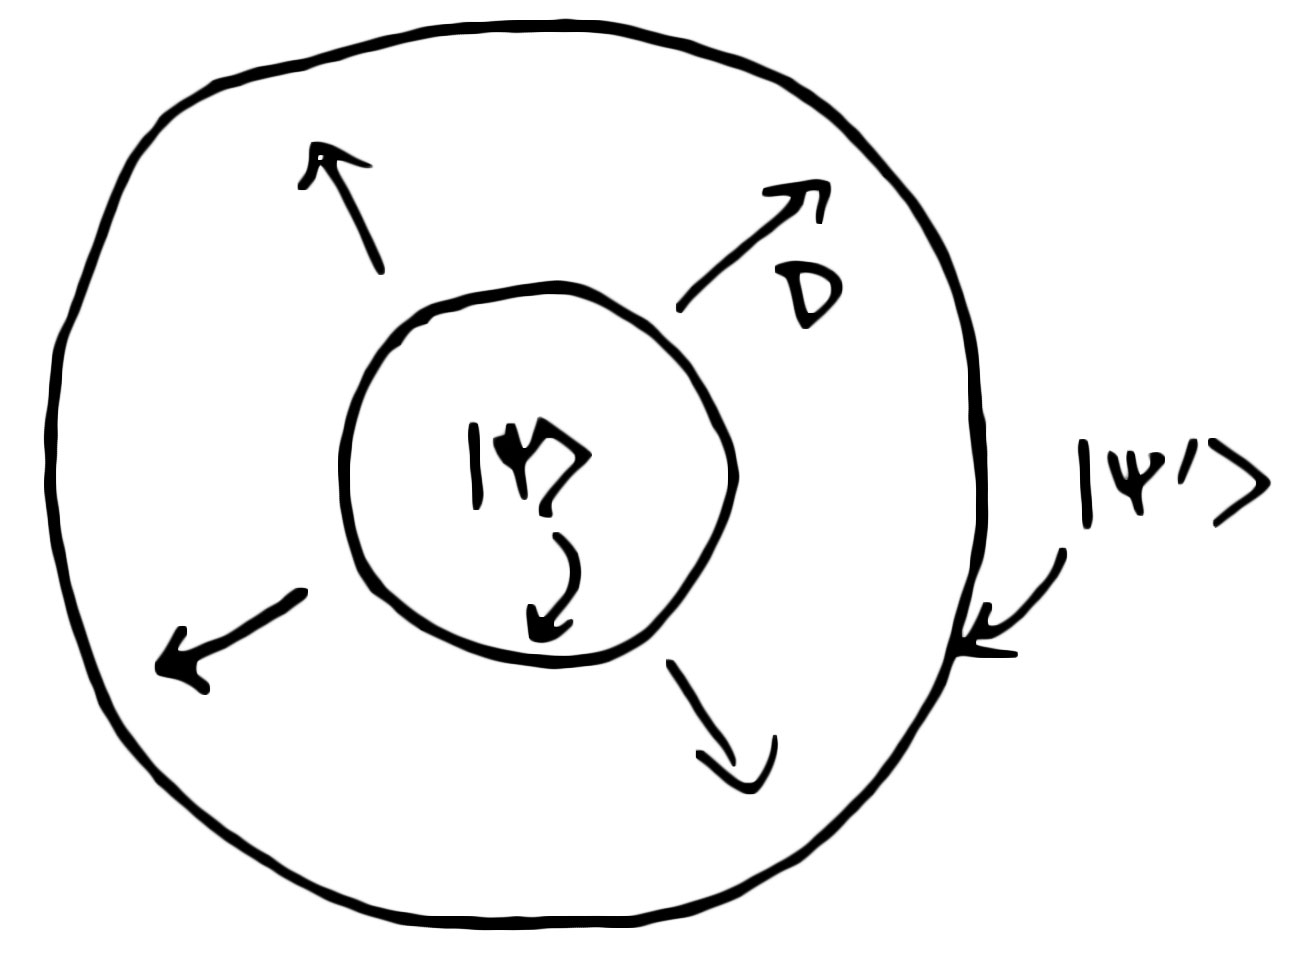
\includegraphics[width=0.35\textwidth]{radialquantization.jpg}
\end{center}
\caption{In radial quantization, states live on spheres, and we evolve from one state to another with the dilatation operator. \label{fig:radialquantization}}
\end{figure}

\begin{figure}
\begin{center}
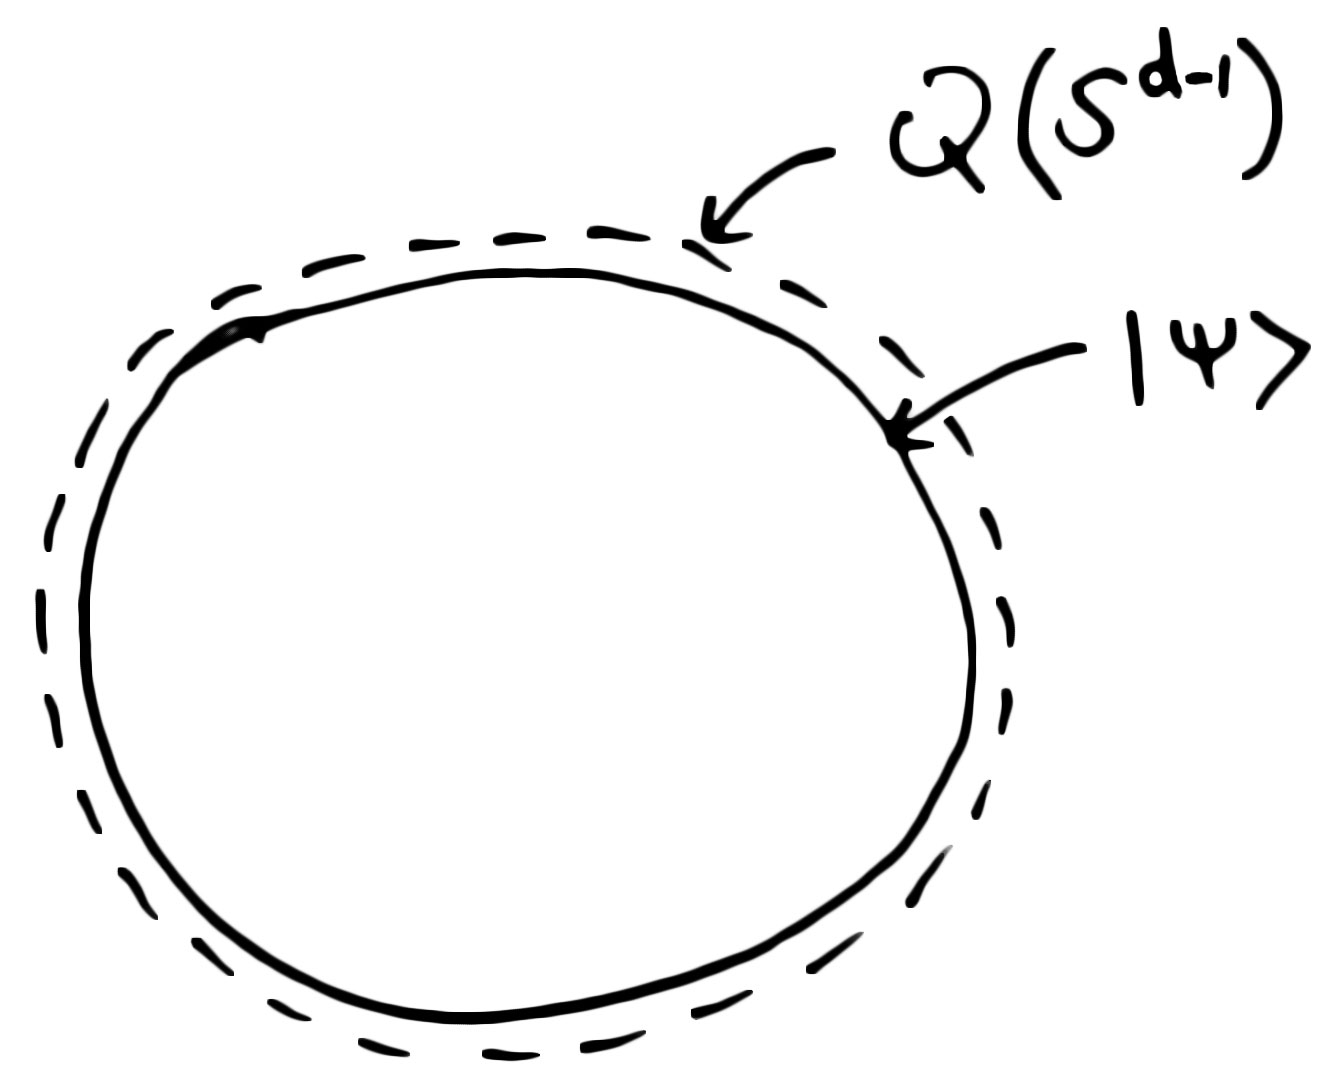
\includegraphics[width=0.35\textwidth]{chargeactionradialquantization.jpg}
\end{center}
\caption{We act with a charge in radial quantization by inserting $Q(S^{d-1})$ just outside the sphere on which the state is defined. \label{fig:chargeactionradialquantization}}
\end{figure}

In radial quantization, a correlation function gets interpreted as a radially ordered product,
\be
\<\cO_1(x_1)\cdots \cO_n(x_n)\> &= \<0|\mathcal{R}\{ \cO_1(x_1)\cdots \cO_n(x_n)\}|0\>\nn\\
&\equiv  \theta(|x_n|-|x_{n-1})\cdots \theta(|x_2|-|x_1|) \<0|\cO(x_n)\cdots\cO(x_1)|0\>\nn\\
&+\mathrm{permutations}.
\ee
Of course, we can perform radial quantization around different points.  The same correlation function then gets interpreted as an expectation value of differently ordered operators acting on different states in different (but isomorphic) Hilbert spaces (figure~\ref{fig:radialquantdifferentpoints}).  This is completely analogous to changing reference frames in Lorentz invariant theories.  The radial ordering prescription is consistent because operators at the same radius but different angles on the sphere commute, just as spacelike-separated operators commute in the usual quantization.

\begin{figure}
\begin{center}
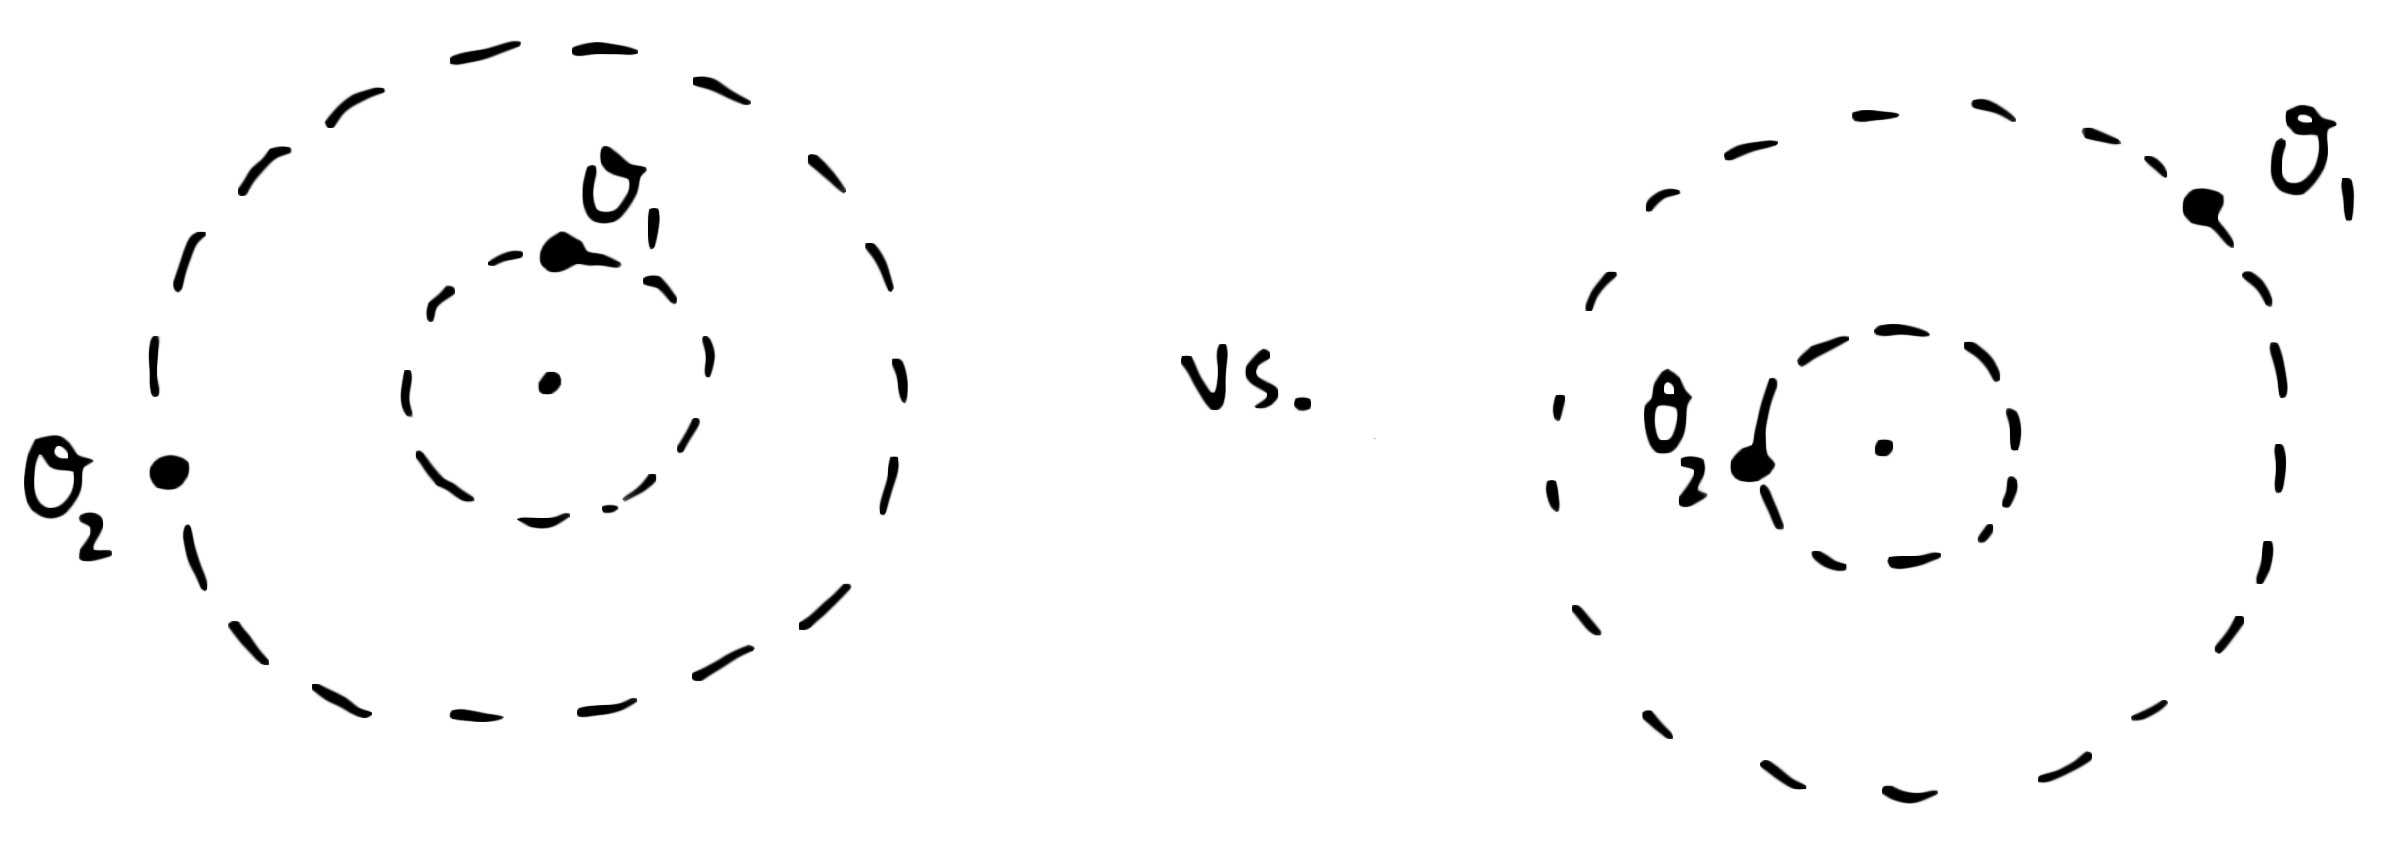
\includegraphics[width=0.75\textwidth]{radialquantdifferentpoints.jpg}
\end{center}
\caption{When we perform radial quantization around different points, the same correlator gets interpreted as a product of operators with different orderings.  \label{fig:radialquantdifferentpoints}}
\end{figure}

\subsection{Operator $\Longrightarrow$ state}
\label{sec:operatorimpliesstate}

The simplest way to prepare a state in radial quantization is to perform the path integral over the interior $B$ of the sphere, with no operator insertions inside $B$.  This gives the vacuum state $|0\>$ on the boundary $\ptl B$ (figure~\ref{fig:radialvacuum.jpg}).  It's easy to see that $|0\>$ is invariant under all symmetries because a topological surface on the boundary of $B$ can be shrunk to zero inside $B$ (figure~\ref{fig:vacuuminvariant}).

\begin{figure}
\begin{center}
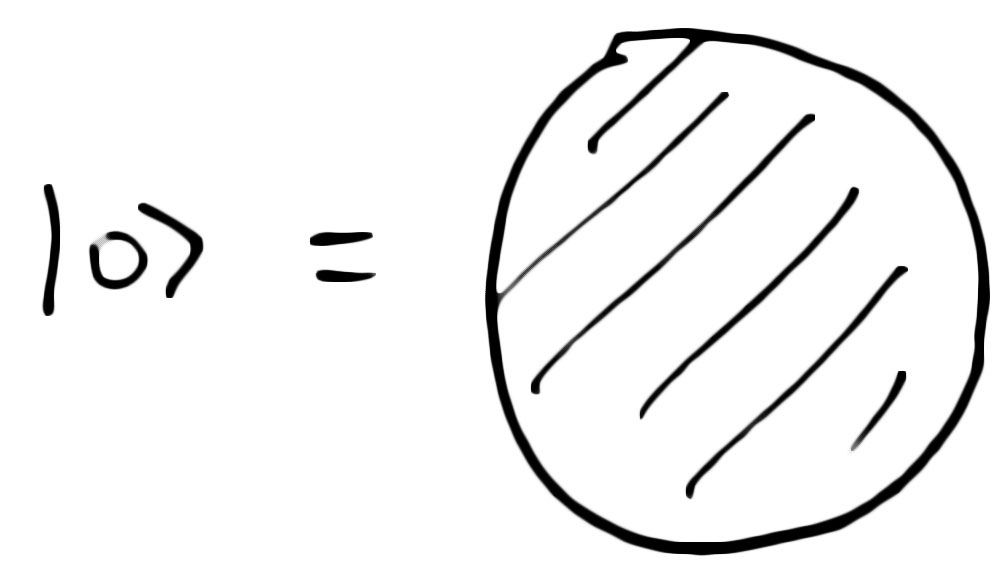
\includegraphics[width=0.3\textwidth]{radialvacuum.jpg}
\end{center}
\caption{The vacuum in radial quantization is given by the path integral over the interior of the sphere, with no operator insertions.  \label{fig:radialvacuum.jpg}}
\end{figure}

\begin{figure}
\begin{center}
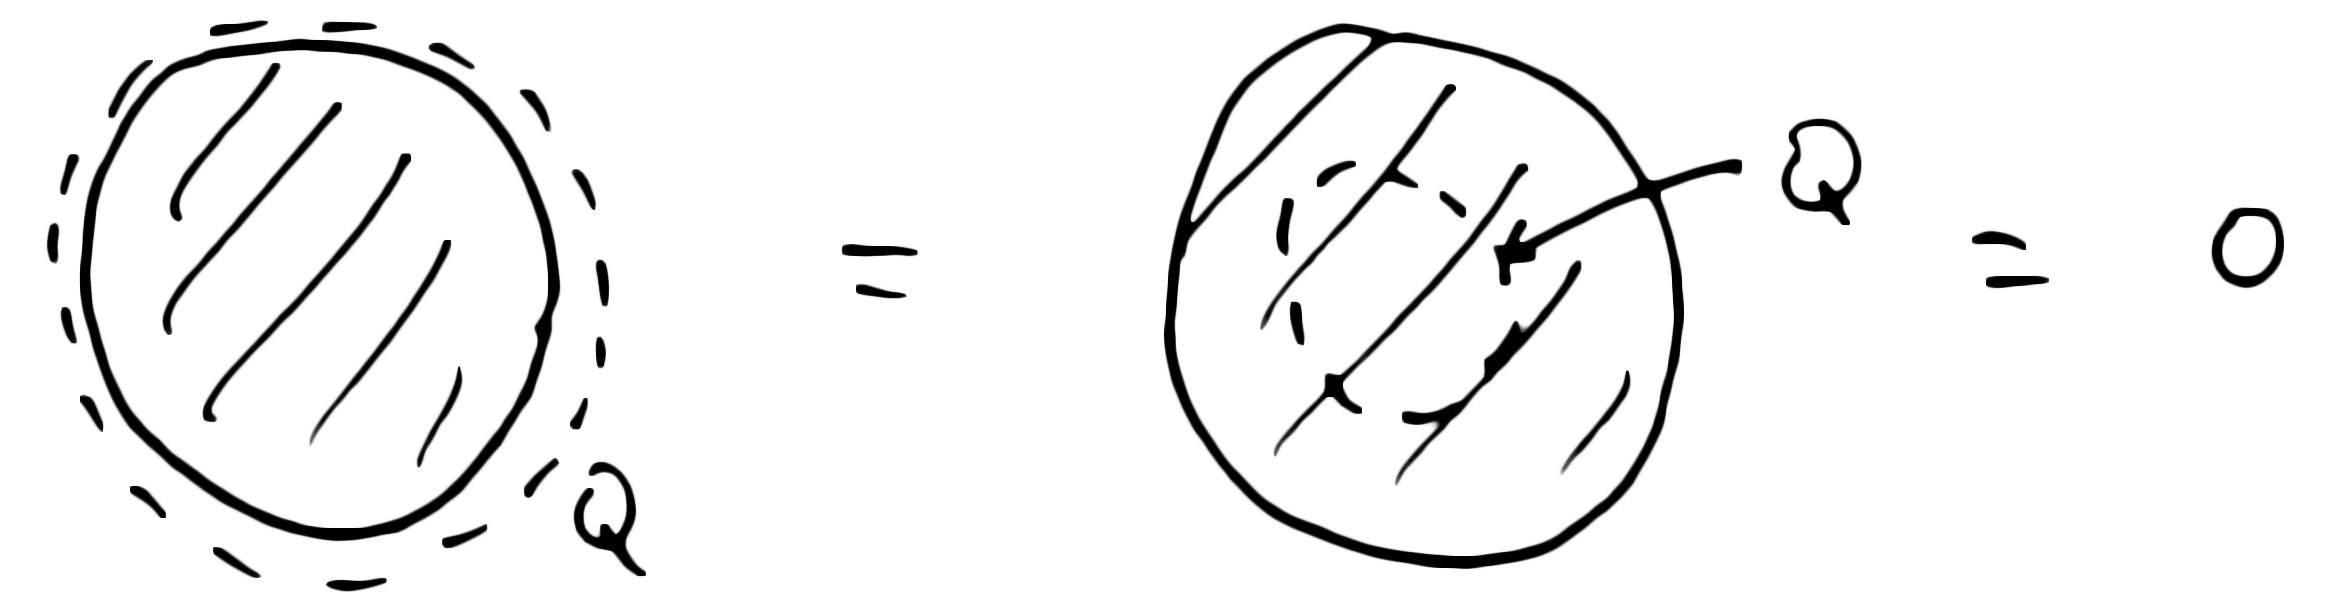
\includegraphics[width=0.7\textwidth]{vacuuminvariant.jpg}
\end{center}
\caption{The vacuum is automatically invariant under all symmetries.  \label{fig:vacuuminvariant}}
\end{figure}

To be explicit, suppose our CFT is given by the path integral over a scalar field $\phi$.  The Hilbert space in radial quantization is spanned by ``field eigenstates" $|\phi_b\>$, where $\phi_b(\bn)$ is a field configuration on the sphere $\bn\in \ptl B$.  The subscript ``$b$" indicates that $\phi_b$ is defined only on the boundary $\ptl B$ and not in the interior.  A general state is a linear combination of field eigenstates
\be
|\psi\> &\equiv \int D\phi_b |\phi_b\>\<\phi_b|\psi\>.
\ee
Here, $\int D\phi_b$ represents a $d-1$-dimensional path integral over fields on $\ptl B$.

For the vacuum, the coefficients $\<\phi_b|0\>$ are given by the path integral over the interior with boundary conditions $\phi_b$ and no operator insertions,
\be
\<\phi_b |0\> &=  \int_{\substack{\phi(1,\bn)=\phi_b(\bn) \\ r \leq 1}} D\phi(r,\bn) e^{-S[\phi]}.
\ee

A more exciting possibility is to insert an operator $\cO(x)$ inside $B$ and then perform the path integral,
\be
\<\phi_b|\cO(x)|0\> &= \int_{\substack{\phi(1,\bn)=\phi_b(\bn) \\ r \leq 1}} D\phi(r,\bn) \cO(x) e^{-S[\phi]}.
\ee
This defines a state called $\cO(x)|0\>$, see figure~\ref{fig:radialexcited}.
By inserting different operators inside $B$, we can prepare a variety of states on the boundary $\ptl B$. In this language, $|0\>$ is prepared by inserting the unit operator.

\begin{figure}
\begin{center}
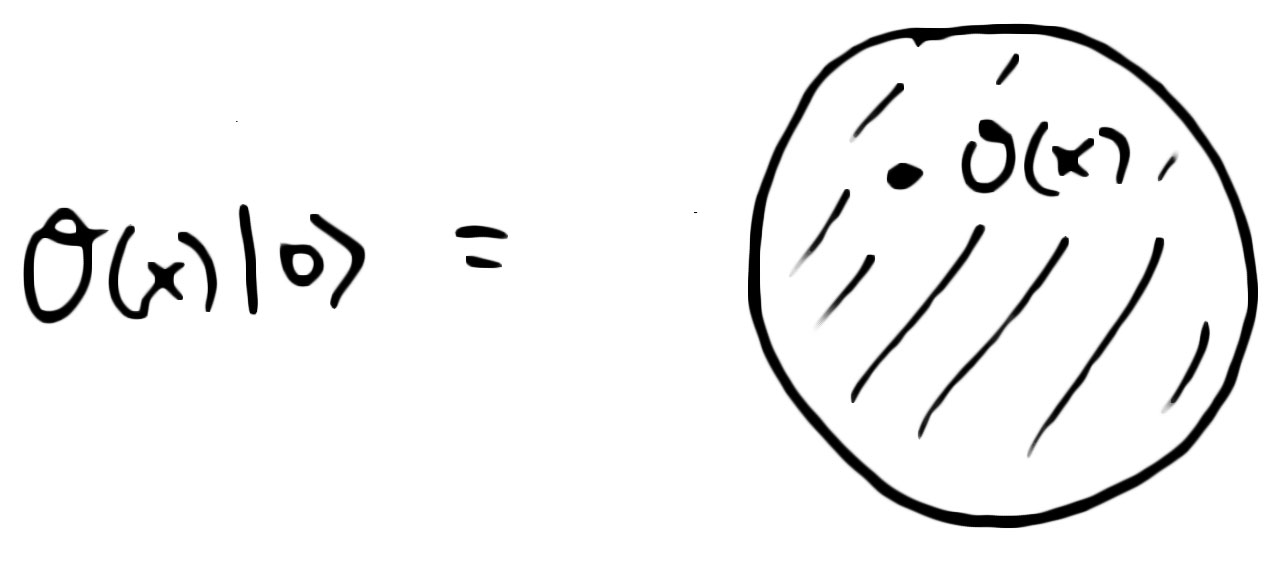
\includegraphics[width=0.4\textwidth]{radialexcited.jpg}
\end{center}
\caption{The state $\cO(x)|0\>$ is given by inserting $\cO(x)$ inside the sphere and performing the path integral over the interior.  \label{fig:radialexcited}}
\end{figure}

\subsection{Operator $\Longleftarrow$ state}

This construction also works backwards. Let $|\cO_i\>$ be eigenstates of the dilatation operator
\be
\label{eq:eigenvectorofD}
D |\cO_i\> &= \De_i |\cO_i\>.
\ee
%  Given a state $|\psi\>$ in radial quantization, let us decompose it into eigenstates of the dilatation operator,
%\be
%|\psi\> &= |\cO_1\>+|\cO_2\>+\dots\\
%D|\psi\> &= \De_1|\cO_1\>+\De_2|\cO_2\>+\dots.
%\ee
The $|\cO_i\>$ can themselves be used as operators: we cut spherical holes $B_i$ out of the path integral centered around positions $x_i$ and glue in the states $|\cO_i\>$ at the boundary of the holes, as in figure~\ref{fig:correlatorofstates}.
\begin{figure}
\begin{center}
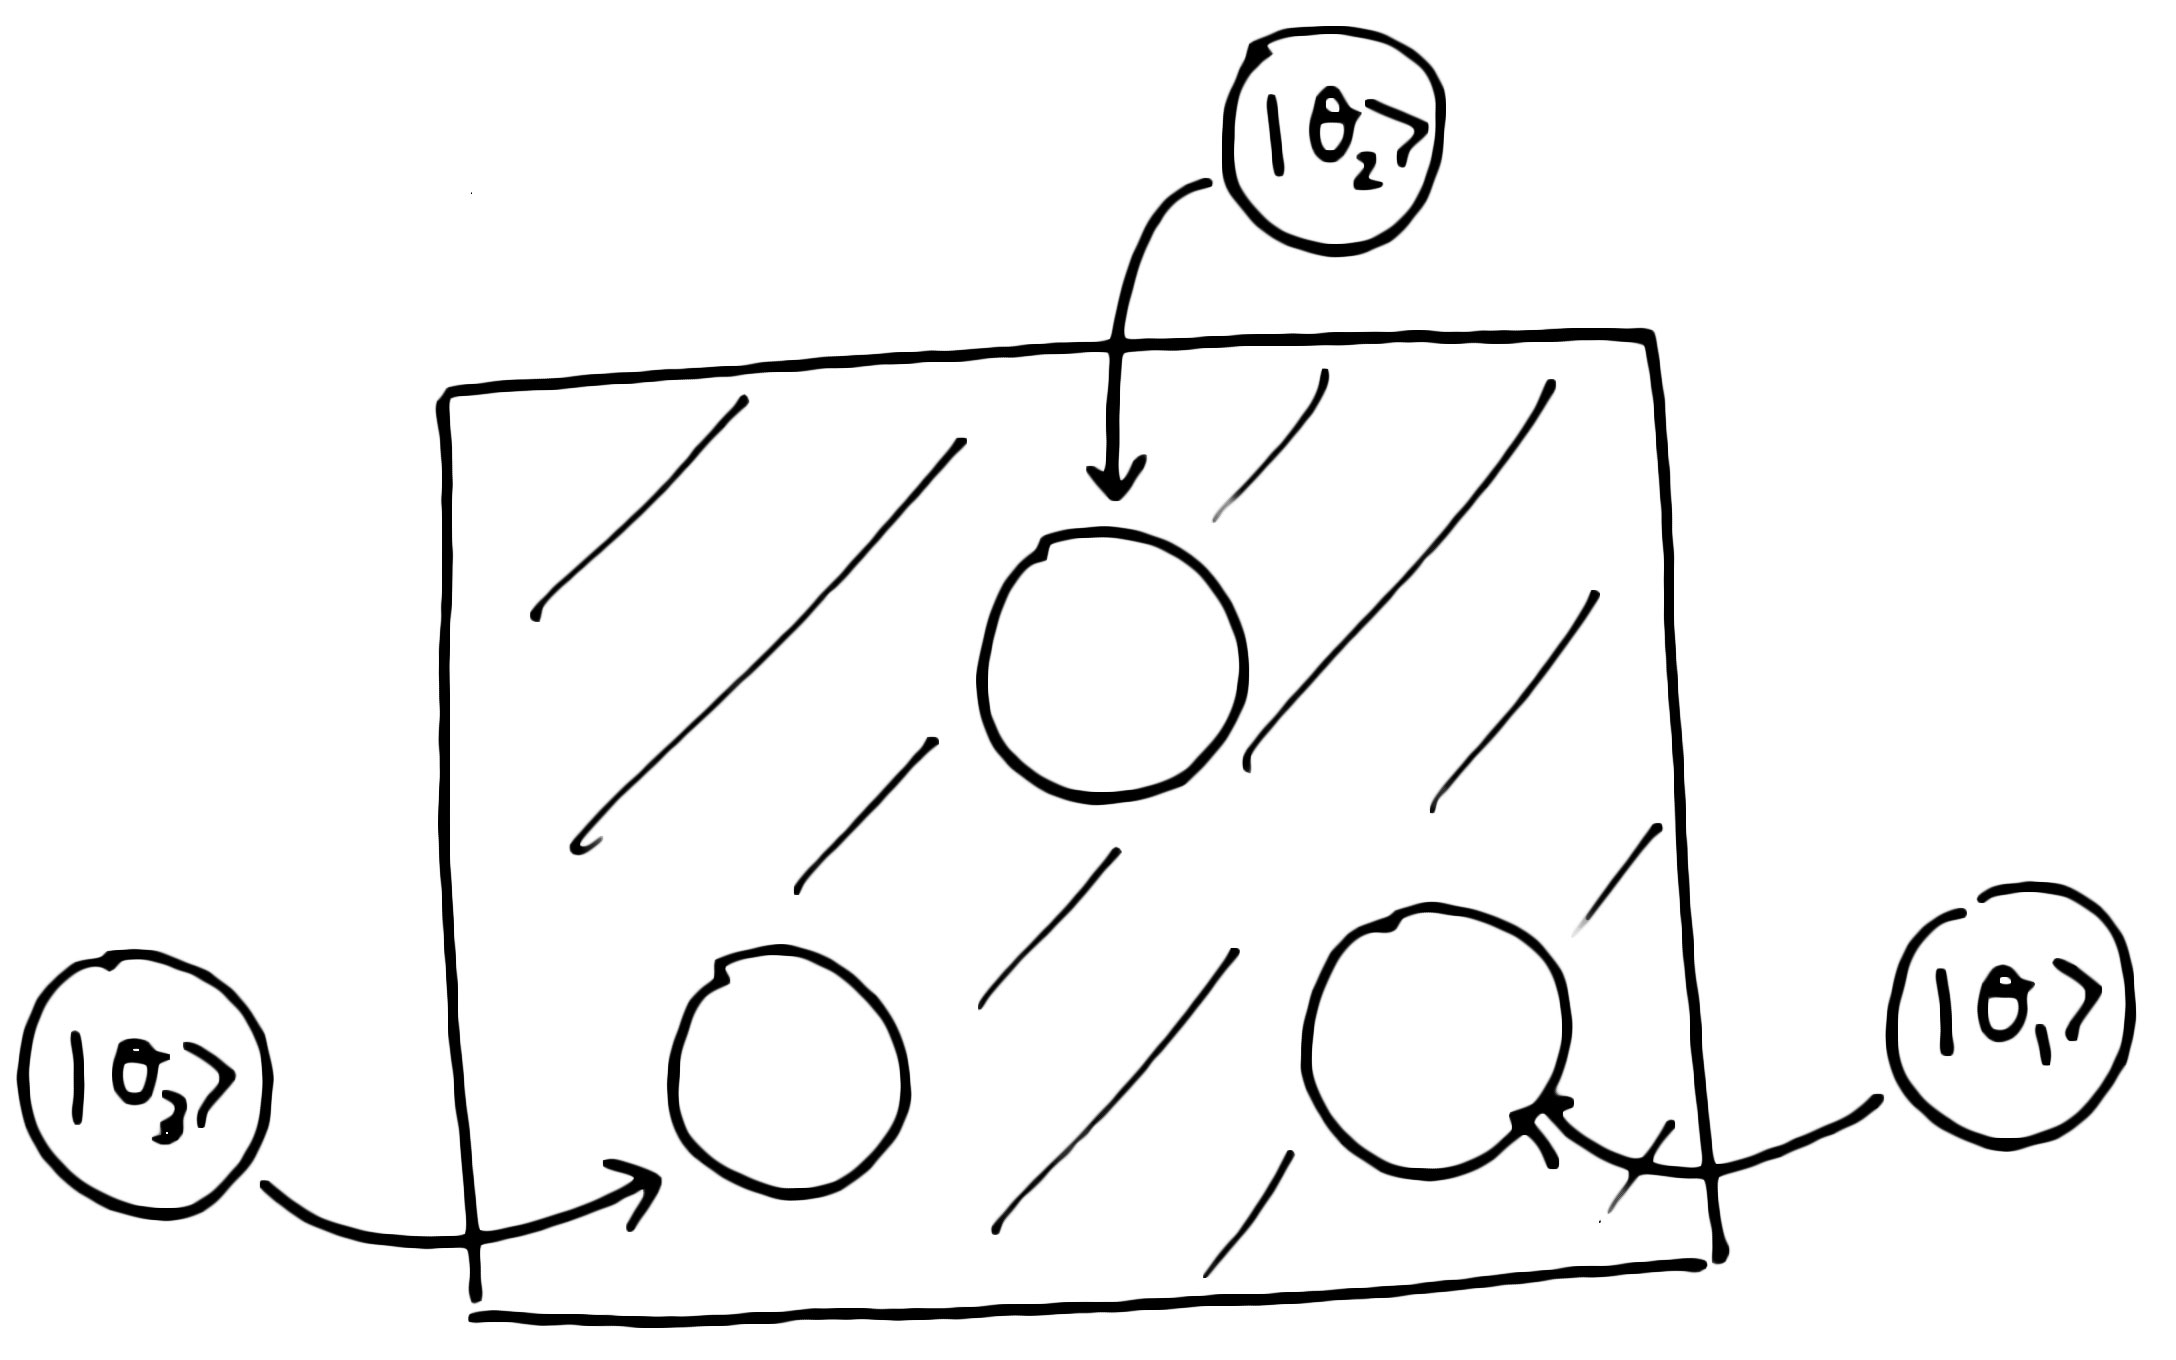
\includegraphics[width=0.7\textwidth]{correlatorofstates.jpg}
\end{center}
\caption{A correlator of states is defined by cutting holes out of the path integral and gluing states into the holes.  \label{fig:correlatorofstates}}
\end{figure}
This gives a quantity that behaves exactly like a correlator of local operators.
In the scalar field example, the gluing procedure gives an object
\be
\label{eq:pathintegralforC}
C\p{|\cO_1\>, x_1;\dots ;|\cO_n\>, x_n} &\equiv \int \prod_i D\phi_{bi} \<\phi_{bi}|\cO_i\> \int_{\substack{\phi_{\ptl i}=\phi_{bi}\\ x \notin B_i }} D\phi(x)\, e^{-S[\phi]},
\ee
where the path integral $D\phi(x)$ is performed over the region outside the balls $B_i$, and the integrals $D\phi_{bi}$ are over field configurations on the boundaries $\ptl B_i$. Here, $\phi_{\ptl i}$ denotes the restriction of the bulk field $\phi(x)$ to the $i$-th boundary $\ptl B_i$.

This construction only works when the $x_i$ are far enough apart that the balls $B_i$ don't overlap. However, a correlator of local operators should make sense for arbitrary configurations of non-coincident points. To overcome this problem, we can use the fact that we have diagonalized the dilatation operator. Let us define a correlator of the states $|\cO_i\>$ by using a dilatation to bring the spheres far enough apart,
\be
\label{eq:definitionofstatecorrelator}
\<\cO(x_1)\cdots \cO(x_n)\> &\equiv \lambda^{\sum_i \Delta_i} C(|\cO_1\>, \l x_1;\dots ;|\cO_n\>, \l x_n),
%\<\cO_1(\lambda x_1)\cdots \cO_n(\lambda x_n)\>,
\ee
where $\l\in \R$ is any number sufficiently large that $\l|x_{ij}|>1$.  Since the $x_i$ can now be arbitrarily close together, we have defined local operators.\footnote{A more careful construction of the state $\implies$ operator map that doesn't require this rescaling trick is given in Polchinski \cite{Polchinski:1998rq} volume 1, chapter 2.}

We should check that (\ref{eq:definitionofstatecorrelator}) doesn't depend on $\l$ (assuming $\l$ satisfies the condition $\l|x_{ij}|>1$). Note that
\be
&\pdr{}{\l} \<\cO(x_1)\cdots \cO(x_n)\> \nn\\
&= \lambda^{\sum_i \Delta_i}\sum_i\p{\De_i + x_i\.\pdr{}{x_i}} C(|\cO_1\>, \l x_1; \dots ;|\cO_n\>, \l x_n)
%&= \lambda^{\sum_i \Delta_i} \sum_i C(|\cO_1\>, \l x_1;\dots; D_i|\cO_i\>,\l x_i; \dots ;|\cO_n\>, \l x_n),
\ee
Because of (\ref{eq:eigenvectorofD}), the latter expression is the same as inserting a topological surface operator for $D$ in the path integral (\ref{eq:pathintegralforC}), which vanishes if we have scale-invariant boundary conditions.
%where
%\be
%D_i &= D + x_i\. P
%\ee

\stoplecture

\subsection{Operator $\Longleftrightarrow$ state}

So far I've been vague about what I mean by a local operator.  But now, we can give a rigorous definition: we will simply {\it define\/} a local operator to be an eigenstate of $D$ in radial quantization.\footnote{The dilatation operator is diagonalizable in unitary (reflection positive) CFTs.  However, there exist interesting non-unitary theories where $D$ has a nontrivial Jordan block decomposition.  In these cases, we define a local operator as a finite-dimensional representation of $D$.} With this definition, the two constructions above are inverse to each other, with the identification
\be
\cO(0)\quad &\longleftrightarrow \quad \cO(0)|0\>\equiv |\cO\>.
\ee
This is the ``state-operator correspondence."

It is straightforward to see how the conformal group acts on states in radial quantization.  A primary operator creates a state that is killed by $K_\mu$ and transforms in a finite-dimensional representation of $D$ and $M_{\mu\nu}$,
\begin{align}
\label{eq:operatortostateconditionK}
\,[K_\mu,\cO(0)]&=0 &\longleftrightarrow &  K_\mu|\cO\>&=0,\\
\label{eq:operatortostateconditionD}
\,[D,\cO(0)] &= \De\cO(0) &\longleftrightarrow & D|\cO\>&=\De|\cO\>,\\
\label{eq:operatortostateconditionM}
\,[M_{\mu\nu},\cO(0)]&=\cS_{\mu\nu}\cO(0) &\longleftrightarrow & M_{\mu\nu}|\cO\> &= \cS_{\mu\nu}|\cO\>.
\end{align}
This follows by acting on $|0\>$ with the operator equations above and using the fact that $|0\>$ is killed by $K,D,$ and $M$.

A conformal multiplet in radial quantization is given by acting with momentum generators on a primary state
\be
|\cO\>, P_\mu|\cO\>, P_\mu P_\nu|\cO\>, \dots \qquad\textrm{(conformal multiplet)}.
\ee
This is equivalent to acting with derivatives of $\cO(x)$ at the origin, for example
\be
\ptl_\mu\cO(x)|_{x=0}|0\> &= [P_\mu,\cO(0)]|0\>=P_\mu|\cO\>.
\ee
The operator $\cO(x)$ creates an infinite linear combination of descendants,
\be
\cO(x)|0\>\ =\  e^{x\.P}\cO(0)e^{-x\.P}|0\>\ =\ e^{x\.P}|\cO\>\ =\ \sum_{n=0}^\oo \frac{1}{n!}(x\.P)^n|\cO\>.\quad
\ee

As with the classification of operators, the action of the conformal algebra on a multiplet in radial quantization is determined by the commutation relations of the algebra. In fact the required computations look {\it exactly identical\/} to the computations we did to determine the action of conformal generators on operators (\ref{eq:actionbyrotation}, \ref{eq:dilatationaction}, \ref{eq:actionofK}).  This is because by surrounding operators with charges supported on spheres, we were secretly doing radial quantization all along!


\subsection{Another view of radial quantization}

To study a conformal Killing vector $\e$, it is often helpful to perform a Weyl rescaling of the metric $g\to \Omega(x)^2 g$ so that $\e$ becomes a regular Killing vector, i.e.\ an isometry.  We can turn a dilatation into an isometry by performing a Weyl rescaling from $\R^d$ to the cylinder $\R\x S^{d-1}$,
\be
ds_{\R^d}^2 &= dr^2 + r^2 ds_{S^{d-1}}^2\nn\\
&= r^2\p{\frac{dr^2}{r^2} + ds_{S^{d-1}}^2}\nn\\
&= e^{2\tau}(d\tau^2 + ds_{S^{d-1}}^2) = e^{2\tau} ds_{\R\x S^{d-1}}^2,
\ee
where $r=e^\tau$.

Dilatations $r\to\l r$ become shifts of radial time $\tau\to\tau+\log \l$.  Radial quantization in flat space is equivalent to the usual quantization on the cylinder.  States live on spheres and time evolution is generated by acting with $e^{-D\tau}$.  While the development of radial quantization in the previous sections relied only on scale invariance, the cylinder picture relies on conformal invariance because we have performed a nontrivial Weyl rescaling.

Let us build a more detailed dictionary between the two pictures.  Under a Weyl rescaling, correlation functions of local operators transform as\footnote{In even dimensions, the partition function itself can transform with a Weyl anomaly $\<1\>_g=\<1\>_{\Omega^2 g}e^{S_\mathrm{Weyl}[g,\Omega]}$.  This will not be important for our discussion, so we have divided through by the partition function.}
\be
\label{eq:weyltransformation}
\frac{\<\cO_1(x_1)\cdots\cO_n(x_n)\>_g}{\<1\>_g} &= \p{\prod_i \Omega(x_i)^{\De_i}}\frac{\<\cO_1(x_1)\cdots\cO_n(x_n)\>_{\Omega^2g}}{\<1\>_{\Omega^2 g}}.
\ee
This is a nontrivial claim --- if we implement the Ising model in flat space, compute expectation values and take the continuum limit, it's not obvious that the answer should be simply related to the same lattice theory on the cylinder.\footnote{Comparing the flat and cylindrical Ising models is relatively easy in 2d, but harder in 3d since $S^2$ is curved. See \cite{Brower:2014gsa} for a recent attempt.}    In general it isn't, but at the critical value of the coupling when the theory becomes conformal, tracelessness of the stress tensor implies insensitivity to Weyl rescalings, and the answers become related.

\begin{exercise}
By integrating by parts in (\ref{eq:dilatationaction}), show that 
\be
\label{eq:tracetcontact}
T_\mu^\mu(x) \cO(y) &= \De \de(x-y)\cO(y).
\ee
An insertion of $T_\mu^\mu$ is the response of the theory to an infinitesimal Weyl transformation $g\to e^{2\de\omega} g$. Derive (\ref{eq:weyltransformation}) by exponentiation.\footnote{We cheated here by only deriving (\ref{eq:tracetcontact}) in flat space.  In curved space there is an additional contribution to $T_\mu^\mu$ coming from the Weyl anomaly.  This factor cancels in (\ref{eq:weyltransformation}). There could also be modifications to the contact term (\ref{eq:tracetcontact}). However, in a conformally flat metric, we can simply define the curved space operator $\cO(x)$ so that it satisfies (\ref{eq:tracetcontact}). For instance, we may modify the Weyl factor so that it is constant in a tiny neighborhood of $\cO(x)$ and the flat-space calculation applies. This definition might not be consistent with other independent definitions. For instance, if $\cO(x)$ is the stress tensor, it gives a different answer from the canonical definition (\ref{eq:definitionofstresstensor}) because of the Weyl anomaly.}
\end{exercise}

Thus, given an operator $\cO(x)$ in $\R^d$, it is natural to define a cylinder operator
\be
\label{eq:definitionofcylinderop}
\cO_\mathrm{cyl.}(\tau,\bn) &\equiv e^{\De \tau} \cO_\mathrm{flat}(x=e^\tau \bn).
\ee
We often omit the subscripts ``cyl." and ``flat," relying on the coordinates to indicate which type of operator we're discussing.
\begin{exercise}
Using (\ref{eq:weyltransformation}), compute a two-point function of cylinder operators
\be
\<\cO(\tau_1,\bn_1)\cO(\tau_2,\bn_2)\>.
\ee
Verify that it is time-translationally invariant on the cylinder. Show that in the limit of large time separation $\tau=\tau_2-\tau_1 \gg 1$, the two-point function has an expansion in terms of the form $e^{-(\De+n)\tau}$ with integer $n\geq 0$.  Interpret these as coming from the exchange of states in the conformal multiplet of $\cO$.
\end{exercise}

\section{Reflection positivity and unitarity bounds}

\subsection{Reflection positivity}
\label{sec:reflectionpositivity}

In Lorentzian signature, we are interested in unitary theories: theories where the conserved charges (including the Hamiltonian) are Hermitian operators so that they generate unitary transformations.  Unitarity in Lorentzian signature is equivalent to a property called ``reflection positivity" in Euclidean signature.\footnote{We make some brief comments about Euclidean vs. Lorentzian field theory and analytic continuation in appendix~\ref{app:analyticcontinuation}.}

Consider a Lorentzian theory with a local operator $\cO_L$ and Hermitian energy-momentum generators $(H,\bP_L)$ ($L$ is for ``Lorentzian").  We have the textbook formula
\be
\label{eq:textbookinlorentz}
\cO_L(t,\bx) &= e^{iHt-i\bx\.\bP_L}\cO_L(0,0)e^{-iHt+i\bx\.\bP_L}.
\ee
Let $\cO_L(0,0)$ be Hermitian.  It follows from (\ref{eq:textbookinlorentz}) that $\cO_L(t,\bx)$ is Hermitian too.

Now, let us Wick-rotate to Euclidean signature,
\be
\label{eq:wickrotatedoperator}
\cO_E(t_E,\bx) \equiv \cO_L(-it_E,\bx)
= e^{Ht_E-i\bx\.\bP_L}\cO_L(0,0)e^{-Ht_E+i\bx\.\bP_L}.
\ee
The Euclidean operator satisfies
\be
\cO_E(t_E,\bx)^\dag &= \cO_E(-t_E,\bx).
\ee
To Wick-rotate an operator with spin, we conventionally add factors of $-i$ to the time components,\footnote{These factors are needed to make Euclidean correlation functions manifestly covariant under $\SO(d)$ rotations.} e.g.\ for a vector operator $\cO_L^\mu$,
\be
\label{eq:factorsofIinWick}
\cO_E^0(t_E,\bx) &= -i \cO_L^0(-it_E,\bx),\nn\\
\cO_E^i(t_E,\bx) &= \cO_L^i(-it_E,\bx).
\ee
This leads to
\be
\label{eq:reflectionforhermitianconjugation}
\cO_E^{\mu_1\dots\mu_\ell}(t_E,\bx)^\dag &= \Theta^{\mu_1}{}_{\nu_1}\cdots \Theta^{\mu_\ell}{}_{\nu_\ell} \cO_E^{\nu_1\cdots\nu_\ell}(-t_E,\bx),
\ee
where $\Theta^\mu{}_\nu = \de^\mu_\nu-2\de^\mu_0\de_\nu^0$ is a reflection in the time-direction.

Thus, the way Hermitian conjugation acts on a Euclidean operator depends on which direction we call time.  Whether an operator is Hermitian or not depends on how we quantize the theory! This is very different from Lorentzian signature, where the conjugation properties of operators don't depend on a choice of reference frame.

\stoplecture

As an example, consider the momentum generators
\be
P^\mu &= -\int d^{d-1}\bx\, T^{\mu 0}(0,\bx).
\ee
(From now on, we work in the Euclidean theory and omit the $E$ subscripts.)
Using (\ref{eq:reflectionforhermitianconjugation}), we have
\be
T^{i 0}(0,\bx)^\dag &= -T^{i0}(0,\bx),\nn\\
T^{00}(0,\bx)^\dag &= T^{00}(0,\bx).
\ee
It follows that $P^0$ is Hermitian, and the $P^i$ are {\it antihermitian}.  We may write
\be
P^0 = H,\qquad
P^j = -iP^j_L,
\ee
with $H,P_L$ Hermitian, and then (\ref{eq:integratedtranslations}) agrees with the formula we got from Wick rotation (\ref{eq:wickrotatedoperator}).  If we had quantized with a different time direction, say the $x_1$-direction, then we would conclude that $P^1$ is Hermitian, while $P^0,P^2,\dots,P^{d-1}$ are antihermitian.

To reiterate, {\it the way conjugation acts on operators depends on how we quantize our theory}.  This makes sense, because Hermitian conjugation is something you do to operators on Hilbert spaces, and different quantizations have different Hilbert spaces.

This raises the question: given a Euclidean path integral, how do we know if it computes the Wick-rotation of a unitary Lorentzian theory?  One important condition is that norms of states should be positive.  Consider some in-state $|\psi\>$ given by acting on the vacuum with a bunch of operators at negative Euclidean time
\be
|\psi\> &= \cO(-t_{E1})\cdots\cO(-t_{En})|0\>.
\ee
For brevity, we suppress the spatial positions of the operators.
The conjugate state is given by
\be
\<\psi| &= (\cO(-t_{E1})\cdots\cO(-t_{En})|0\>)^\dag \nn \\
&= \<0|\cO(t_{En})\cdots\cO(t_{E1}).
\ee
That is, $\<\psi|$ is given by taking the vacuum in the future and positioning operators in a time-reflected way.  Thus, the condition
\be
\<\psi|\psi\> &\geq 0
\ee
says that a time-reflection symmetric configuration should have a positive path integral, see figure~\ref{fig:reflectionpositivity}.  This is called ``reflection positivity."

\begin{figure}
\begin{center}
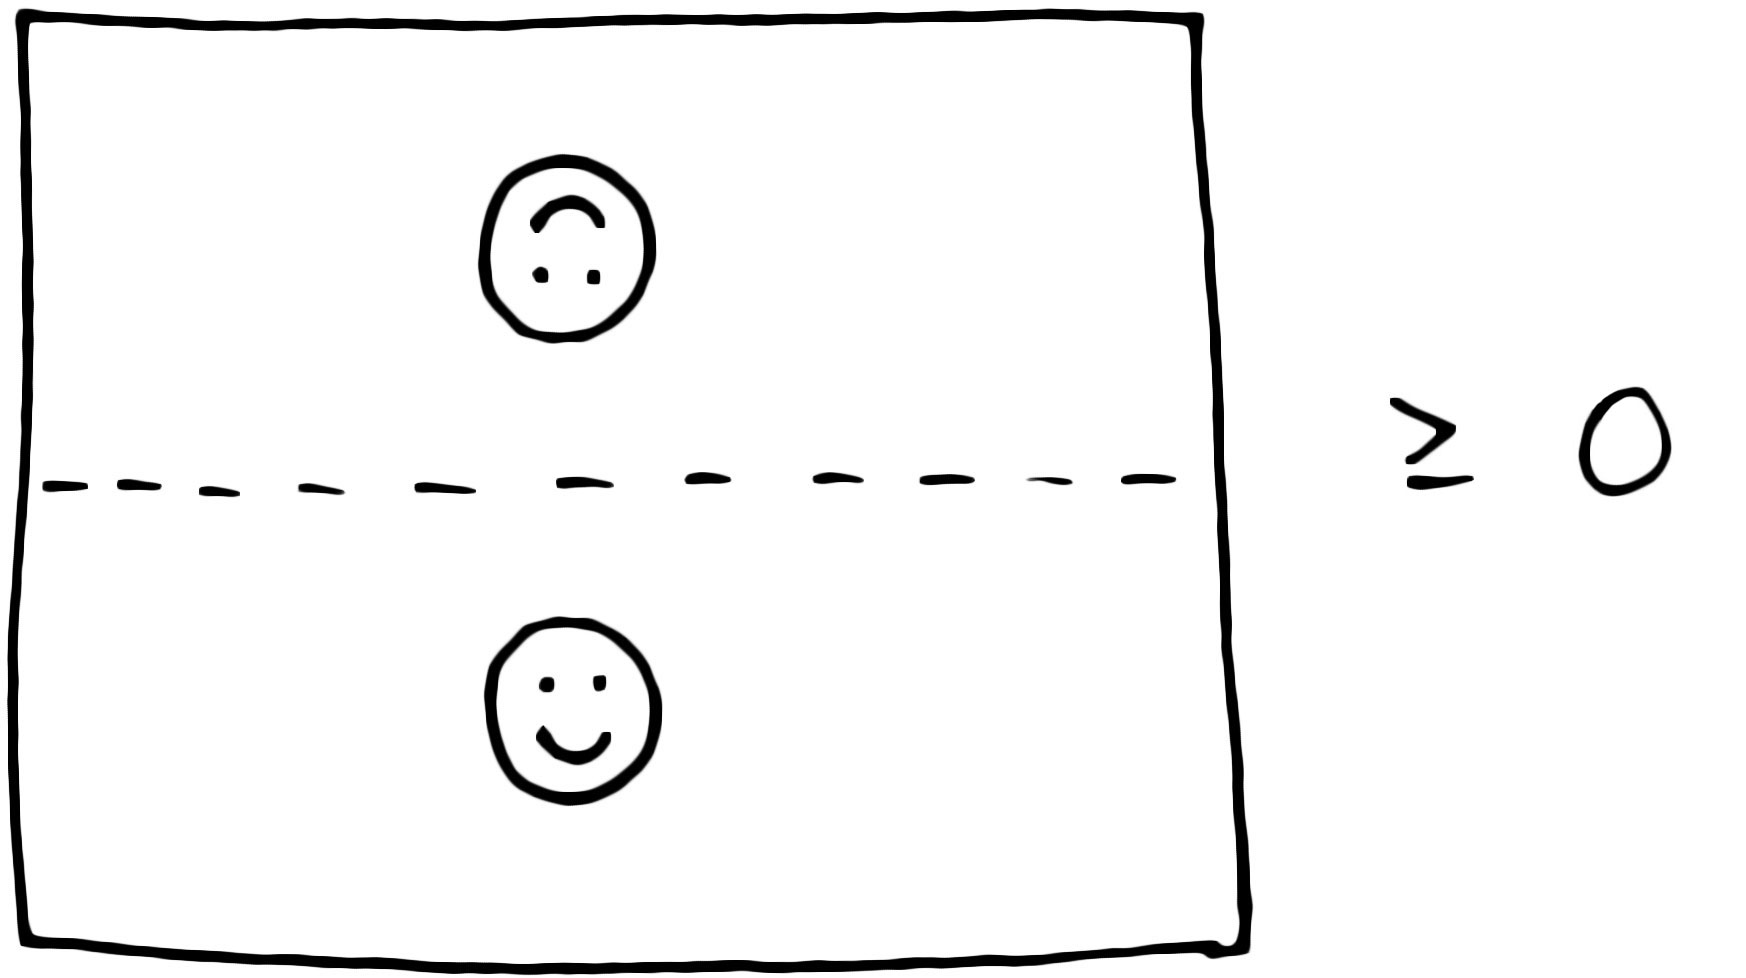
\includegraphics[width=0.5\textwidth]{reflectionpositivity.jpg}
\end{center}
\caption{Reflection positivity.  \label{fig:reflectionpositivity}}
\end{figure}

If a Euclidean theory is the Wick-rotation of a unitary Lorentzian theory, then it will be reflection positive.  However, some theories are more naturally defined in Euclidean signature.  In this case, reflection positivity must be checked.  It often suffices to check it in any microscopic theory in the same universality class as the CFT we're interested in.
\begin{exercise}
Consider the 2d Ising lattice correlator shown in figure~\ref{fig:isingreflectioncorrelator}.  Show that it can be written as a sum of squares, and is hence positive. (Hint: first sum over spins off the line $L$, and then sum over spins on $L$.) Generalize your proof to argue that the 2d Ising model is reflection-positive.
\end{exercise}

\begin{figure}
\begin{center}
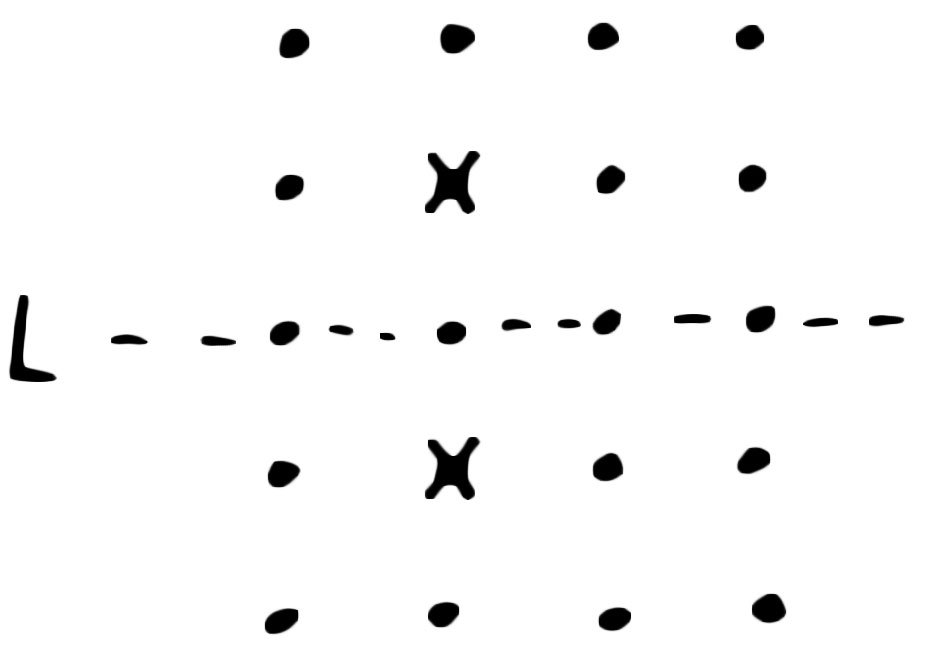
\includegraphics[width=0.3\textwidth]{isingreflectioncorrelator.jpg}
\end{center}
\caption{A two point function on a $4\x 5$ Ising lattice with free boundary conditions, with spin operators  inserted at the sites marked with an X.  \label{fig:isingreflectioncorrelator}}
\end{figure}

The Osterwalder-Schrader reconstruction theorem says that, given a collection of Euclidean correlators satisfying reflection positivity (and some additional technical assumptions), we can reconstruct a unitary Lorentzian quantum field theory by analytic continuation \cite{GlimmJaffe}.  So reflection positivity in Euclidean signature and unitarity in Lorentzian signature are essentially equivalent, and we will use the terms interchangeably. 

\subsubsection{Real vs.\ complex operators}
\label{sec:realvscomplex}

Because Hermitian conjugation is tricky in Euclidean signature, it is helpful introduce some extra terminology.  We call a local operator ``real" if it is Hermitian in Lorentzian signature.  In Euclidean signature, real operators satisfy (\ref{eq:reflectionforhermitianconjugation}).  By contrast, for a complex operator $\cO_L^\dag = \cO_L^*$, we have
\be
\label{eq:complexoperatorconjugation}
\cO_E^{\mu_1\dots\mu_\ell}(t_E,\bx)^\dag &= \Theta^{\mu_1}{}_{\nu_1}\cdots \Theta^{\mu_\ell}{}_{\nu_\ell} \cO_E^{\nu_1\cdots\nu_\ell*}(-t_E,\bx).
\ee

%We will often use the following convention: 
%\begin{itemize}
%\item A dagger on the operator name itself $\cO^\dag(t_E,\bx)$ means we take the conjugate at the origin first and then translate it to $(t_E,\bx)$.
%\item A dagger on the outside means conjugation after translation, like we've been discussing above.
%\end{itemize}
%With these conventions, we can write (\ref{eq:complexoperatorconjugation}) as
%\be
%\label{eq:complexoperatorconjugation}
%\cO_E^{\mu_1\dots\mu_\ell}(t_E,\bx)^\dag &= \Theta^{\mu_1}{}_{\nu_1}\cdots \Theta^{\mu_\ell}{}_{\nu_\ell} \cO_E^{\nu_1\cdots\nu_\ell}^\dag(-t_E,\bx).
%\ee

Later we will need the following result.
If $\f_1,\f_2$ are real scalars and $\cO$ is a real operator with spin $\ell$ in a unitary theory, then the three-point coefficient $f_{\f_1\f_2\cO}$ is real. This is easiest to see in Lorentzian signature when the operators are spacelike separated $x_{ij}^2>0$. Because local operators commute at spacelike separation, we have
\be
\<0|\f_1(x_1)\f_2(x_2) \cO^{\mu_1\cdots\mu_\ell}(x_3)|0\>^* &= \<0|\f_1(x_1)\f_2(x_2) \cO^{\mu_1\cdots\mu_\ell}(x_3)|0\>.\quad
\ee
Substituting (\ref{eq:scalarscalarspinL}) gives $f_{\f_1\f_2\cO}^*=f_{\f_1\f_2\cO}$.

\subsection{Reflection positivity on the cylinder}
\label{sec:reflposcyl}

Reflection-positivity (or unitarity) has interesting consequences for CFTs on the cylinder.  The Hermitian conjugate of a real cylinder operator is
\be
\cO_\mathrm{cyl.}(\tau,\bn)^{\dag_\mathrm{rad}} &= \cO_\mathrm{cyl.}(-\tau,\bn).
\ee
Using (\ref{eq:definitionofcylinderop}), this becomes
\be
\cO_\mathrm{flat}(x)^{\dag_\mathrm{rad}} &= x^{-2\De}\cO_\mathrm{flat}\p{\frac{x^\mu}{x^2}}.\label{eq:radialconjugation}
\ee
Above, we have written $\dag_\mathrm{rad}$ to emphasize that Hermitian conjugation in radial quantization is different from Hermitian conjugation in the usual $P^0$ quantization.  From now on we write simply $\dag$, and hope that the meaning will be clear from context.

The right-hand side of (\ref{eq:radialconjugation}) is just the image of $\cO(x)$ under an inversion $I:x^\mu\to \frac{x^\mu}{x^2}$.  The same is true for operators with spin, where the full formula (\ref{eq:finiteprimarytransformation}) gives
\be
\label{eq:conjugateforspin}
\cO^{\mu_1\cdots\mu_\ell}(x)^\dag &= I^{\mu_1}{}_{\nu_1}(x)\cdots I^{\mu_\ell}{}_{\nu_\ell}(x) x^{-2\De} \cO^{\nu_1\dots\nu_\ell}\p{\frac{x}{x^2}},\nn\\
I^\mu{}_\nu(x) &= \de^\mu_\nu - \frac{2 x^\mu x_\nu}{x^2}.
\ee
\begin{exercise}
Check that the two-point function of spin-1 operators (\ref{eq:finalresultforVV}) satisfies reflection-positivity on the cylinder if $c_{12}>0$.
\end{exercise}
Applying (\ref{eq:conjugateforspin}) to the stress tensor, we find that 
 the action of conjugation on the conformal charges in radial quantization is
\be
Q_\e^\dag &= -Q_{I\e^{*\nu}I^{-1}}.
\ee
Here, $I\e^{*\nu}I^{-1}$ is defined by its action on functions $f(x)$. The action of $I$ on functions is given by $(If)(x)=f(I(x))$.
The minus sign comes from the fact that the unit normal vector $x^\mu/|x|$ used in defining the charges flips sign under an inversion.
In particular, we have
\be
\label{eq:mantihermitian}
M_{\mu\nu}^\dag &= -M_{\mu\nu},\nn\\
D^\dag &= D,\nn\\
P_\mu^\dag &= K_\mu.
\ee

These facts let us calculate properties of correlation functions purely algebraically.  As an example, consider a two-point function.  Letting $\tl y = y/y^2$, we have
\be
\<\cO(y)\cO(x)\> &= \<0|(y^{-2\De}\cO(\tl y))^\dag \cO(x)|0\>\nn\\
&= y^{-2\De}\<0|(e^{\tl y\.P}\cO(0)e^{-\tl y\.P})^\dag e^{x\.P}\cO(0)e^{-x\.P}|0\>\nn\\
&= y^{-2\De}\<0|e^{-\tl y\.K}\cO(0)^\dag e^{\tl y\.K} e^{x\.P}\cO(0)e^{-x\.P}|0\>\nn\\
&= y^{-2\De}\<0|\cO(0)^\dag e^{\tl y\.K} e^{x\.P}\cO(0) |0\>\nn\\
&= y^{-2\De}\<\cO|e^{\tl y\.K} e^{x\.P}|\cO\>,
\label{eq:twopointfromalgebra}
\ee
where we've defined
\be
\label{eq:bpzconjugatescalar}
\<\cO| \equiv \<0|\cO(0)^\dag = \lim_{y\to \oo} y^{2\De} \<0|\cO(y).
\ee
By expanding the exponentials, we can evaluate (\ref{eq:twopointfromalgebra}) using the conformal algebra.  For example, the first couple terms are
\be
\<\cO(y)\cO(x)\> &= y^{-2\De}\p{\<\cO|\cO\> + \frac{y^\mu}{y^2}x^\nu\<\cO|K_\mu P_\nu|\cO\>+\dots},
\ee
where we've used that $K|\cO\>=\<\cO|P=0$ because $\cO$ is primary.  Using the conformal commutation relations,
\be
\<\cO|K_\mu P_\nu|\cO\> &= \<\cO|[K_\mu,P_\nu]|\cO\>\nn\\
&= \<\cO|(2D\de_{\mu\nu}-2M_{\mu\nu})|\cO\>\nn\\
&= 2\De\de_{\mu\nu}\<\cO|\cO\>.
\label{eq:normoffirstdescendant}
\ee
Thus,
\be
\<\cO(y)\cO(x)\> &= y^{-2\De} \<\cO|\cO\>\p{1 + 2\De\frac{y\.x}{y^2}+\dots}.
\ee
This exactly matches the expansion of $\<\cO|\cO\>/(x-y)^{2\De}$ in small $|x|/|y|$!  You can imagine computing all the higher terms and matching the whole series expansion.

%Let us also recover our earlier result that a two-point function of operators in different irreducible spin representations must vanish.  Consider a primary operator $\cO^a$ transforming in a nontrivial unitary representation of $\SO(d)$. The dual state transforms in the dual representation, so we will write it with a lowered index $(|\cO^a\>)^\dag=\<\cO_a|$.  Consider the matrix element $\<\cO_a|M_{\mu\nu}|\cO^b\>$.  Using that $M_{\mu\nu}$ is antihermitian (\ref{eq:mantihermitian}), we can act with it on both the bra and the ket:
%\begin{align}
%-((\cS_{\mu\nu})_c{}^a)^*\<\cO_c|\cO^b\> = \<\cO_a|M_{\mu\nu}|\cO^b\> = \<\cO_a|\cO^c\>(\cS_{\mu\nu})_c{}^b.
%\end{align}
%But $\cS_{\mu\nu}$ is antihermitian as well, so as a matrix equation this says
%\be
%\cS_{\mu\nu}N=N \cS_{\mu\nu},
%\ee
%where $N_a{}^b\equiv\<\cO_a|\cO^b\>$.  By Schur's lemma, $N_a{}^b$ must vanish if $a$ and $b$ are indices of different irreducible representations.  If $a,b$ are indices for a single irreducible representation, then $N$ is proportional to the identity.

\begin{exercise}
This computation is not directly relevant to the course, but it is instructive for getting used to radial ordering.  Consider a three-point function of scalars
\be
\<\cO_i(x_1)\cO_j(x_2)\cO_k(x_3)\> &= \<0|\mathcal{R}\{\cO_i(x_1)\cO_j(x_2)\cO_k(x_3)\}|0\>\nn\\
&=\theta(|x_3|\geq |x_2| \geq |x_1|)\<0|\cO_k(x_3)\cO_j(x_2)\cO_i(x_1)|0\>\nn\\
&+\mathrm{permutations}.
\ee
Consider the operator $e^{2\pi i\mathcal{D}_1}$ where
\be
\mathcal{D}_1 &= x_1\.\ptl_1+\De_1.
\ee
Using the fact that $e^{2\pi i\mathcal{D}_1}\cO_1(x_1)= e^{2\pi i D}\cO_1(x_1)e^{-2\pi i D}$, compute the action of $e^{2\pi i \mathcal{D}_1}$ on each of the terms above.  You will get different answers for each of the different operator orderings.

Now determine the action of $e^{2\pi i \mathcal{D}_1}$ on the known answer for the scalar three-point function (\ref{eq:conformalthreeptfunction}).  Check that the two answers agree.
\end{exercise}

\stoplecture

\subsubsection{BPZ conjugation}

To generalize this computation, we need to define a bra state $\<\cO|$ in radial quantization for an operator $\cO$ in a general representation $\rho$ of $\SO(d)$. The formula~(\ref{eq:conjugateforspin}) gives the radial conjugate of a tensor operator. In our explanation, the $I^\mu{}_\nu(x)$'s came from factors of $i$ introduced during Wick rotation, e.g.\ (\ref{eq:factorsofIinWick}). However, there is no natural convention for Wick-rotating other representations, e.g.\ spinors.

The correct generalization of (\ref{eq:conjugateforspin}) to arbitrary $\rho$ is
\be
\label{eq:bpzconjugation}
\cO^a(x)^{\dag_\mathrm{rad}} &= \frac{g_{a\bar a}(x)}{x^{2\De}} \cO^{\dag \bar a}\p{\frac{x}{x^2}}.
\ee
Here, $\cO^{\dag \bar a}(y)$ denotes the non-radial Hermitian conjugate of $\cO$ at the origin,\footnote{Note that different choices of time direction at the origin may give different definitions of $\cO^{\dag \bar a}$. However, these choices will cancel out in the combination $g_{a \bar a} \cO^{\dag \bar a}$. Also, the origin is not important here: we could have chosen any reference point $y_0$ and defined $\cO^\dag(y_0)$ in any quantization such that $y_0$ is at zero time.} translated to the point $y$
\be
\cO^{\dag \bar a}(y) &= e^{y\.P}\cO^{\dag \bar a}(0) e^{-y\.P}.
\ee
The tensor $g_{a\bar a}(x)=(g^{\bar a a}(x))^*$ is the inverse of the numerator of a two-point function
\be
\label{eq:twopointandconjugate}
\<\cO^{\dag \bar a}(x_2)\cO^b(x_1)\> &= c_\cO \frac{g^{\bar a b}(x_{12})}{x_{12}^{2\De}},
\ee
normalized so that
\be
\sum_{\bar a}(g^{\bar a a}(x))^* g^{\bar a b} &= \de_a^b.
%g_{a\bar a}(x) g^{\bar a b}(x) &= \de_a^b,
\ee
Here, $c_\cO$ is a positive operator-dependent constant.
Note that (\ref{eq:bpzconjugation}) reduces to (\ref{eq:conjugateforspin}) when $\cO$ is a real, traceless symmetric tensor.\footnote{We have written $\dag_\mathrm{rad}$ in (\ref{eq:bpzconjugation}) to emphasize that $\cO^a(x)^{\dag_\mathrm{rad}}$ and $\cO^{\dag b}(x)$ are different. You will often see people drop the ``rad" and simply distinguish between the two objects by whether $\dag$ is on the outside or inside of the parentheses. This notation can be very confusing, but is sometimes convenient.\label{footnote:confusing}} The definition (\ref{eq:bpzconjugation}) is called Belavin-Polyakov-Zamolodchikov (BPZ) conjugation.

Let us make some comments about (\ref{eq:twopointandconjugate}).  Recall from section~\ref{} that $\cO(x)$ can only have a nonzero two-point function with an operator in the dual reflected representation $(\rho^R)^*$ of $\SO(d)$. It turns out that $\cO^\dag(x)$ always transforms in this representation. In other-words, we can always find a nonzero conformally-invariant two-point structure (\ref{eq:twopointandconjugate}). This must be the case because $\<0|\cO^\dag \cO|0\>$ is the norm of a state, so it had better be nonzero.

We can also understand this more explicitly. Given a representation $\rho$ of $\SO(d)$, we can form a representation $\rho_L$ of $\SO(d-1,1)$ by
\be
\rho_L(M^L_{\mu\nu}) &= i^{\de_{\mu 0}+\de_{\nu 0}} \rho(M_{\mu\nu}).
\ee
Here $M_{\mu\nu}$ are the generators of $\SO(d)$ and $M^L_{\mu\nu}$ are the generators of $\SO(d-1,1)$.
The factors of $i$ are because of Wick rotation.\footnote{Note that we can naturally Wick-rotate the matrix elements but there is no natural way to Wick-rotate the vectors that $\rho(M)$ acts on, in general.} They ensure that if $\rho(M_{\mu\nu})$ satisfy the algebra of $\SO(d)$, then $\rho_L(M_{\mu\nu}^L)$ satisfy the algebra of $\SO(d-1,1)$. Taking the complex conjugate of both sides, we find
\be
\rho_L(M^L_{\mu\nu})^* &= (-i)^{\de_{\mu 0}+\de_{\nu 0}} \rho(M_{\mu\nu})^*\nn\\
&= i^{\de_{\mu 0}+\de_{\nu 0}} \rho(I_\mu{}^\rho I_{\nu}{}^\s M_{\rho \s})^*,
\ee
where $I_\mu{}^\nu$ is a reflection in the $0$ direction. On the left-hand side are matrix elements acting on $\cO^\dag$ in Lorentzian signature, so $\rho(I_\mu{}^\rho I_{\nu}{}^\s M_{\rho \s})^*$ are matrix elements acting on $\cO^\dag$ in Euclidean signature. Because $\SO(d)$ is compact, complex conjugation is the same as taking the dual. Recalling the definition~(\ref{eq:reflectedrep}), we see that $\rho(I_\mu{}^\rho I_{\nu}{}^\s M_{\rho \s})^*$ are matrix elements of the dual reflected representation $(\rho^R)^*$.

As an example, in exercise~\ref{eq:reflectedreps} we saw that the dual reflected representation of a left-handed spinor $\psi_\a$ in 4d is a right-handed spinor $\bar\psi_{\dot \a}$ (reflected is the same as dual reflected in this case, since each type of spinor in 4d is self-dual). In Lorentzian signature, these representations are indeed complex conjugates of each other.

We are now ready to define the dual state to $|\cO^a\>$ in radial quantization:
\be
\<\cO_a| 
&= (\cO^a(0)|0\>)^{\dag_\mathrm{rad}} \nn\\
&= \lim_{x\to 0} (\cO^a(x)|0\>)^{\dag_\mathrm{rad}} \nn\\
&= \lim_{x\to 0} \<0|\cO^a(x)^{\dag_\mathrm{rad}} \nn\\
&= \lim_{y\to \oo} y^{2\De} g_{ab}(y) \<0|\cO^{\dag b}(y),
\ee
where $y=x/x^2$.
We have given $\<\cO_a|$ a lowered index because it transforms in the dual representation $\rho^*$. A nice property of BPZ conjugation is that the limit $\<\cO_a|$ is independent of the direction along which we take $\cO^\dag$ to infinity. We can see this by computing an inner product
\be
\label{eq:bpznormprim}
\<\cO_b|\cO^a\> &= \lim_{y\to \oo} y^{2\De} g_{b\bar a}(y) \<0|\cO^{\dag \bar a}(y) \cO^a(0)|0\> \nn\\
&= \lim_{y\to \oo} y^{2\De} g_{b\bar a}(y) c_\cO \frac{g^{\bar a a}(y)}{y^{2\De}} \nn\\
&= c_\cO \de_b^a.
\ee

\begin{exercise}
\textbf{\textit{Warning: trick question!}} Let $\cO(x)$ be a Hermitian operator. Recall that 
\be
\label{eq:trickyequation}
[D,\cO(0)] &= \De \cO(0),
\ee
with $\De$ real.
Furthermore, in radial quantization, we have $D^\dag = D$. Now note that the commutator of two Hermitian operators is anti-hermitian:
\be
[A,B]^\dag &= [B,A] = -[A,B].
\ee
How can this be consistent with (\ref{eq:trickyequation})? Hint: see footnote~\ref{footnote:confusing}.
\end{exercise}

\subsection{Unitarity bounds}

Thinking about the theory on the cylinder gives a natural inner product on states in radial quantization.  Unitarity (or reflection positivity) implies that the norms of states must be nonnegative.  By demanding positivity for every state in a conformal multiplet, we obtain bounds on dimensions of primary operators \cite{Mack:1975je,Jantzen,Minwalla:1997ka}.  We have already seen an example in (\ref{eq:normoffirstdescendant}). We found
\be
|P_0|\cO\>|^2 = \<\cO|K_0 P_0|\cO\> = 2\De\<\cO|\cO\>.
\ee
Unitarity implies $\De\geq 0$.

Let us generalize this argument to the case where $\cO^a$ transforms in a nontrivial representation of $\SO(d)$. We can normalize $\cO$ so that
\be
\<\cO_b|\cO^a\> &= \de^a_b.
\ee
Taking inner products between first-level descendants and using the conformal algebra, we find
\be
(P_\mu|\cO^a\>)^\dag P^\nu|\cO^b\> = \<\cO_a|K_\mu P^\nu|\cO^b\>
= 2\De\de_{\mu}^{\nu}\de_a^b-2(\cS_{\mu}{}^{\nu})_a{}^b.\label{innerproduct}
\ee
The state $P^\nu|\cO^b\>$ lives in the representation $\myng{(1)}\otimes \rho$ of $\SO(d)$, where $\myng{(1)}$ is the vector representation.
Unitarity implies that (\ref{innerproduct}) must be positive-definite as a matrix acting on this space.  This implies
\be
\De\geq \textrm{max-eigenvalue}((\cS_{\mu}{}^{\nu})_a{}^b).
\ee
Let us write
\be
(\cS_{\mu}{}^{\nu})_a{}^b &=  \frac 1 2\sum_{\a,\b} (L^{\a\b})_{\mu}{}^{\nu}(\cS_{\a\b})_a{}^b \nn\\
&= \sum_{\substack{A=\a\b \\ \a<\b}} (L^A)_\mu{}^\nu (\cS_A)_a{}^b,\nn\\
(L^{\a\b})_{\mu\nu} &\equiv \de^\a_\mu\de^\b_\nu - \de^\a_\nu\de^\b_\mu,
\ee
where $(L^{\a\b})_{\mu}{}^{\nu}$ is the generator of rotations in the vector representation $\myng{(1)}$. In the second line, we have written $A=\a\b$ with $\a<\b$, which we should think of as an adjoint index of $\SO(d)$. Thinking of $L^A,\cS_A$ as operators on $\myng{(1)}\otimes \rho$, this becomes
\be
\sum_A L^A \otimes \cS_A &= \frac 1 2 \p{(L\otimes 1 +1\otimes \cS)^2-(L\otimes 1)^2 -(1\otimes\cS)^2}\nn\\
&= \frac 1 2\p{-C_2(\myng{(1)}\otimes \rho)+C_2(\myng{(1)})\otimes 1+1\otimes C_2(\rho)},
\ee
where we've used the familiar trick from basic quantum mechanics to get a linear combination of quadratic Casimir operators. (The quadratic Casimir is $-L^2=-\sum_A L^A L_A$ because our generators are antihermitian and differ from the conventional ones by a factor of $i$.)

Let's specialize to the case where $\rho= V_\ell$ is the spin-$\ell$ traceless symmetric tensor representation.  $V_\ell$ has Casimir 
\be
C_2(V_\ell)=\ell(\ell+d-2).
\ee
To get the maximal eigenvalue of $L\.\cS$, we need the minimal Casimir of
\be
\myng{(1)}\otimes V_\ell=V_{\ell-1}\oplus \dots\qquad(\ell>0).
\ee
Here the ``$\dots$" are irreducible representations with larger Casimirs.  Thus,
\be
\De &\geq \frac 1 2\p{-C_2(V_{\ell-1})+C_2(\myng{(1)})+C_2(V_\ell)}\nn\\
&= \ell+d-2.
\ee
This computation was valid only for $\ell> 0$, since for scalars $\myng{(1)}\otimes V_{\ell=0}=V$.

One can also consider more complicated descendants.
\begin{exercise}
Compute the norm of $P_\mu P^\mu |\cO\>$, where $\cO$ is a scalar.  Show that unitarity implies either $\De=0$ or $\De\geq \frac{d-2}{2}$.  This gives a stronger condition than what we derived above ($\De\geq 0$) for scalars.
\end{exercise}

For traceless symmetric tensors in general conformal field theories, these inequalities are the best you can do (other descendants give no new information).\footnote{An elegant way to study all possible descendants at once is to go to momentum space in Lorentzian signature \cite{}. In fact, this is how unitarity bounds were originally derived by Mack. Unfortunately, this direction would take us too far afield from our discussion.}  In theories with more symmetry, like supersymmetric theories or 2d CFTs, unitarity bounds can be more interesting.  A classic reference for unitarity bound computations is \cite{Minwalla:1997ka}.  In the math literature, unitarity bounds for higher-dimensional CFTs were essentially computed long ago by Jantzen \cite{Jantzen}, though the relevance of that work for physics has only been emphasized recently \cite{Yamazaki:2016vqi,Penedones:2015aga}.

In summary, we have the unitarity bounds
\be
\De &= 0 \ \textrm{(unit operator), or}\nn\\
\De &\geq \begin{cases}
\frac{d-2}{2} & \ell = 0,\\
\ell+d-2 & \ell > 0.
\end{cases}
\label{eq:unitaritysummary}
\ee


\subsubsection{Null states and conserved currents}

If $\De$ saturates the bounds (\ref{eq:unitaritysummary}), the conformal multiplet will have a null state.  For the unit operator, all descendants are null.  For a scalar with dimension $\frac{d-2}{2}$, the null state is
\be
P^2|\cO\> &= 0.
\ee
In operator language, this says $\ptl^2 \cO(x)=0$, which means $\cO$ satisfies the Klein-Gordon equation, and is thus a free scalar that decouples from the rest of the CFT.

For a spin-$\ell$ operator, the null state is\footnote{The null state has spin $\ell-1$ because the unitarity bound came from $V_{\ell-1}\subset V\otimes V_\ell$.  Something special happens for vectors in 2d, where $V\otimes V = \mathbf{1}\oplus\mathbf{1}\oplus V_{2}$, with the extra $\mathbf{1}$ appearing because of the antisymmetric $\e_{\mu\nu}$ symbol. Unitarity then implies that $J^{\mu}$ and $\e^{\mu\nu}J_\nu$ are each separately conserved.}
\be
P_\mu | \cO^{\mu\mu_2\cdots\mu_\ell}\> &= 0.
\ee
In operator language, this becomes the equation for a conserved current
\be
\ptl_\mu \cO^{\mu\mu_2\cdots\mu_\ell}(x) &= 0.
\ee
The implication also works the other way:
\be
\label{eq:thmaboutconserved}
\De = \ell + d-2 \qquad \textrm{if and only if}\qquad \textrm{$\cO$ is a conserved current}.
\ee
Some important examples are global symmetry currents ($\ell=1$, $\Delta=d-1$) and the stress tensor ($\ell=2$, $\Delta=d$).  For CFTs in $d\geq 3$, the presence of currents with spin $\ell\geq 3$ implies that the theory is free \cite{Maldacena:2011jn,Boulanger:2013zza,Alba:2015upa}.\footnote{One must also assume the existence of exactly one stress tensor, since otherwise the theory could contain a free subsector, decoupled from the rest.}

\subsection{Only primaries and descendants}
\label{sec:onlyprimariesanddescendants}

With a positive-definite inner product, we can now prove that all operators in unitary CFTs are linear combinations of primaries and descendants. We will use one additional physical assumption: that the partition function of the theory on $S^{d-1}\x S^1_\beta$ is finite,
\be
\mathcal{Z}_{S^{d-1}\x S^1_\beta} = \Tr(e^{-\beta D}) < \oo.
\ee
This means that $e^{-\beta D}$ is trace-class, and hence diagonalizable with a discrete spectrum (by the spectral theorem).\footnote{Assuming $e^{-\b D}$ is trace-class may be too strong for some applications. Boundedness of $e^{-\b D}$ suffices for $D$ to be diagonalizable (with a possibly continuous spectrum). An interesting example is Liouville theory, which has a divergent partition function and continuous spectrum, but still has many properties of a sensible CFT, like an OPE.} It follows that $D$ is also diagonalizable, with real eigenvalues because $D$ is Hermitian.

Now consider a local operator $\cO$, and assume for simplicity it is an eigenvector of dilatation with dimension $\De$.  By finiteness of the partition function, there are a finite number of primary operators $\cO_p$ with dimension less than or equal to $\De$.  Using the inner product, we may subtract off the projections of $\cO$ onto the conformal multiplets of $\cO_p$ to get $\cO'$.  Now suppose (for a contradiction) that $\cO'\neq 0$.  Acting on it with $K_\mu$'s, we must eventually get zero (again by finiteness of the partition function), which means there is a new primary with dimension below $\De$, a contradiction.  Thus $\cO'=0$, and $\cO$ is a linear combination of states in the multiplets $\cO_p$.

\section{The operator product expansion}

If we insert two operators $\cO_i(x)\cO_j(0)$ inside a ball and perform the path integral over the interior, we get some state on the boundary.  Because every state is a linear combination of primaries and descendants, we can decompose this state as
\be
\label{eq:opeinitial}
\cO_i(x)\cO_j(0)|0\> &= \sum_{k}C_{ijk}(x,P)\cO_k(0) |0\>,
\ee
where $k$ runs over primary operators and $C_{ijk}(x,P)$ is an operator that packages together primaries and descendants in the $k$-th conformal multiplet (figure~\ref{fig:ope}).

\begin{figure}
\begin{center}
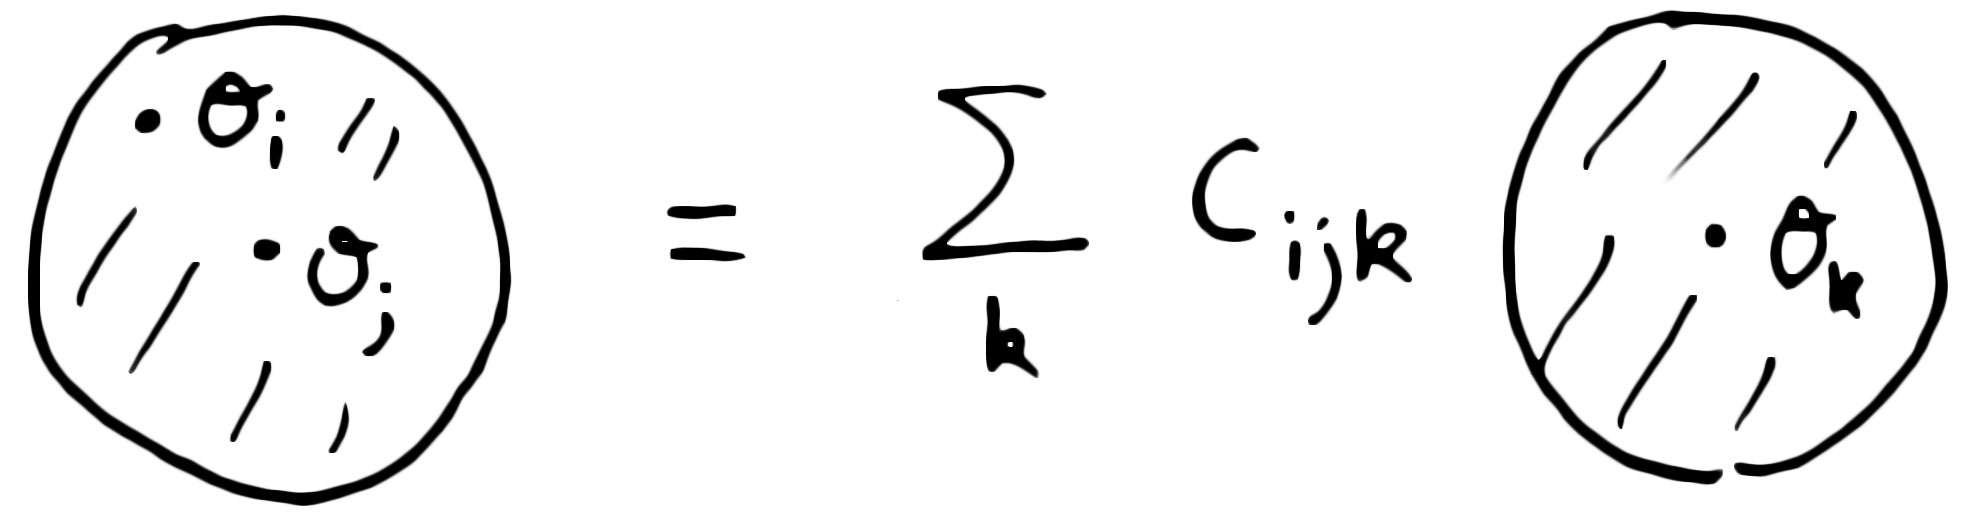
\includegraphics[width=0.6\textwidth]{ope.jpg}
\end{center}
\caption{A state created by two operator insertions can be expanded as a sum of primary and descendant states.  \label{fig:ope}}
\end{figure}

Eq.~(\ref{eq:opeinitial}) is an exact equation that can be used in the path integral, as long as all other operators are outside the sphere with radius $|x|$.  Using the state-operator correspondence, we can write
\be
\label{eq:opeinitial2}
\cO_i(x_1)\cO_j(x_2) &= \sum_{k}C_{ijk}(x_{12},\ptl_2)\cO_k(x_2),\qquad\textrm{(OPE)}
\ee
where it is understood that (\ref{eq:opeinitial2}) is valid inside any correlation function where the other operators $\cO_n(x_n)$ have $|x_{2n}|\geq |x_{12}|$.  Eq.~(\ref{eq:opeinitial2}) is called the Operator Product Expansion (OPE).

We could alternatively perform radial quantization around a different point $x_3$, giving
\be
\label{eq:opealternative}
\cO_i(x_1)\cO_j(x_2) &= \sum_k C'_{ijk}(x_{13},x_{23},\ptl_3)\cO_k(x_3),
\ee
where $C'_{ijk}(x_{13},x_{23},\ptl_3)$ is some other differential operator (figure~\ref{fig:radialquantotherpoint}).  The form  (\ref{eq:opeinitial2}) is usually more convenient for computations, but the existence of (\ref{eq:opealternative}) is important. It shows that we can do the OPE between two operators whenever it's possible to draw any sphere that separates the two operators from all the others.

\begin{figure}
\begin{center}
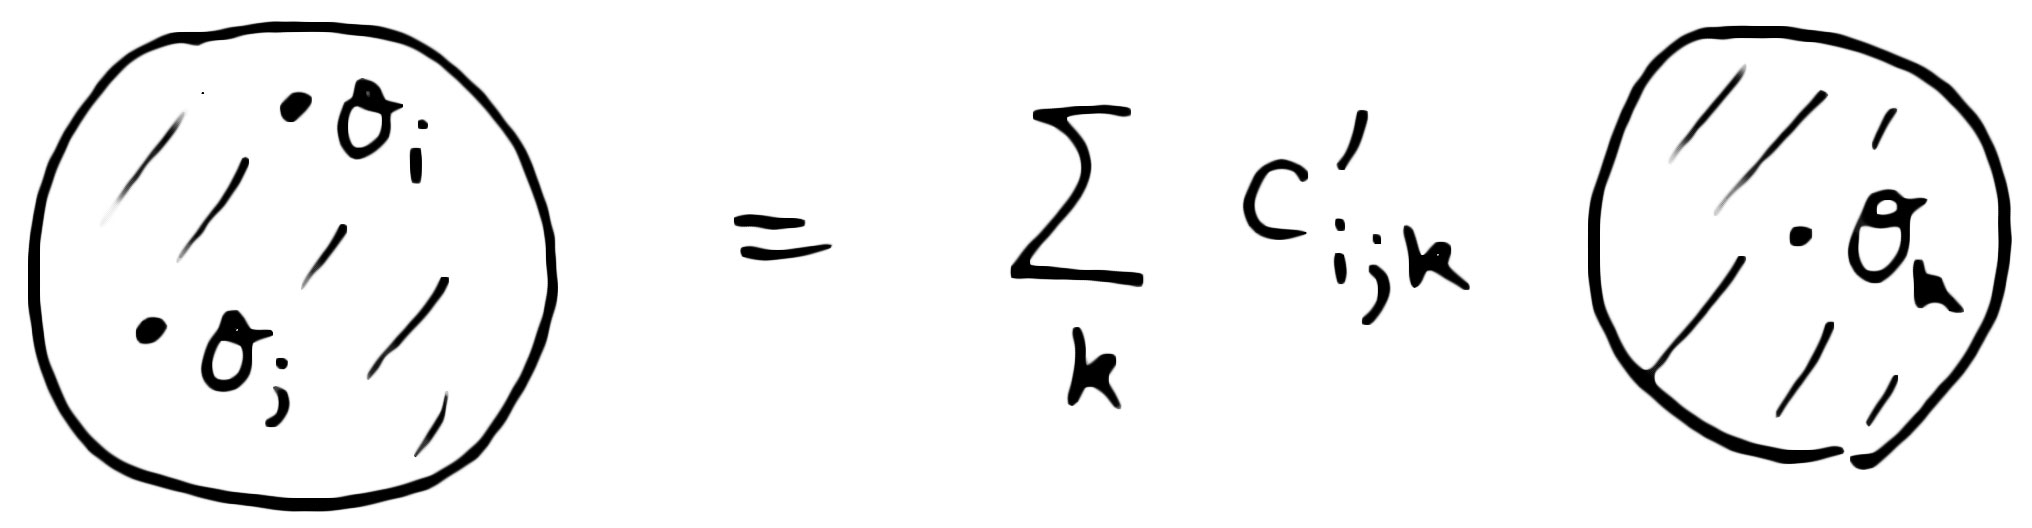
\includegraphics[width=0.6\textwidth]{radialquantotherpoint.jpg}
\end{center}
\caption{It isn't necessary for one of the operators to be at the origin.  \label{fig:radialquantotherpoint}}
\end{figure}

We are being a bit schematic in writing the above equations.  It's possible for all the operators to have spin.  In this case, the OPE looks like
\be
\cO_i^a(x_1)\cO_j^b(x_2) &= \sum_k C_{ijk}^{ab}{}_c(x_{12},\ptl_2)\cO_k^c(x_2),
\ee
where $a,b,c$ are indices for (possibly different) representations of $\SO(d)$.

\subsection{Consistency with conformal invariance}

Conformal invariance strongly restricts the form of the OPE\@.  For simplicity, suppose $\cO_i$, $\cO_j$, and $\cO_k$ are scalars.  
\begin{exercise}
By acting on both sides of (\ref{eq:opeinitial}) with $D$, prove that $C_{ijk}(x,\ptl)$ has an expansion of the form
\be
\label{eq:opeexpansionexample}
C_{ijk}(x,\ptl) &\propto |x|^{\De_k-\De_i-\De_j}\p{1 +\# x^\mu\ptl_\mu + \# x^\mu x^\nu\ptl_\mu\ptl_\nu+\# x^2 \ptl^2 + \dots}.\nn\\
\ee
\end{exercise}
This is just a fancy way of saying we can do dimensional analysis and that $\cO_i$ has length-dimension $-\De_i$. We're also implicitly using rotational invariance by contracting all the indices appropriately. We could have proved this too by acting with $M_{\mu\nu}$.

We get a more interesting constraint by acting with $K_\mu$. In fact, consistency with $K_\mu$ completely fixes $C_{ijk}$ up to an overall coefficient. In this way, we can determine the coefficients in (\ref{eq:opeexpansionexample}).

This computation is a little annoying (exercise!), so here's a simpler way to see why the form of the OPE is fixed, and to get the coefficients in (\ref{eq:opeexpansionexample}).  Take the correlation function of both sides of (\ref{eq:opeinitial2}) with a third operator $\cO_k(x_3)$ (we will assume $|x_{23}|\geq |x_{12}|$, so that the OPE is valid),
\be
\label{eq:threetotwo}
\<\cO_i(x_1)\cO_j(x_2)\cO_k(x_3)\> &= \sum_{k'} C_{ijk'}(x_{12},\ptl_2)\<\cO_{k'}(x_2)\cO_k(x_3)\>.
\ee
The three-point function on the left-hand side is fixed by conformal invariance, and is given in  (\ref{eq:conformalthreeptfunction}). We can choose an orthonormal basis of primary operators, so that $\<\cO_k(x_2)\cO_{k'}(x_3)\>= \de_{kk'}x_{23}^{-2\De_k}$.  The sum then collapses to a single term, giving
\be
\label{eq:matchingthreept}
\frac{f_{ijk}}{x_{12}^{\De_i+\De_j-\De_k}x_{23}^{\De_j+\De_k-\De_i}x_{31}^{\De_k+\De_i-\De_j}} &= C_{ijk}(x_{12},\ptl_2)x_{23}^{-2\De_k}.
\ee
This determines $C_{ijk}$ to be proportional to $f_{ijk}$, times a differential operator that depends only on the $\De_i$'s. The operator can be obtained by matching the small $|x_{12}|/|x_{23}|$ expansion of both sides of (\ref{eq:matchingthreept}).
\begin{exercise}
\label{exercise:seriesfordiffops}
Consider the special case $\De_i=\De_j=\De_\f$, and $\De_k=\De$.  Show
\be
\label{eq:identicalscalaropeoperator}
C_{ijk}(x,\ptl) &= f_{ijk} x^{\De-2\De_\f}\p{1+\frac 1 2 x\.\ptl + \a x^\mu x^\nu\ptl_\mu\ptl_\nu + \b x^2 \ptl^2+\dots},\nn\\
\ee
where
\be
\label{eq:opedescendantcoefficients}
\a &= \frac{\De+2}{8(\De+1)},\quad\textrm{and}\quad \b=-\frac{\De}{16(\De-\frac{d-2}{2})(\De+1)}.
\ee
\end{exercise}

\subsection{Computing correlators with the OPE}

Equation (\ref{eq:threetotwo}) gives an example of using the OPE to reduce a three-point function to a sum of two-point functions.  In general, we can use the OPE to reduce any $n$-point function to a sum of $n-1$-point functions,
\be
\<\cO_1(x_1)\cO_2(x_2)\cdots\cO_n(x_n)\> &= \sum_k C_{12k}(x_{12},\ptl_2)\<\cO_k(x_2)\cdots\cO_n(x_n)\>.\nn\\
\ee
Recursing, we reduce everything to a sum of one-point functions, which are fixed by dimensional analysis,
\be
\<\cO(x)\> &= \begin{cases}
1 & \textrm{if $\cO$ is the unit operator,}\\
0 & \textrm{otherwise.}
\end{cases}
\ee
This gives an algorithm for computing any flat-space correlation function using the OPE\@.  It shows that all these correlators are determined by dimensions $\De_i$, spins, and OPE coefficients $f_{ijk}$.\footnote{The OPE is also valid on any conformally flat manifold.  The difference is that on nontrivial manifolds, non-unit operators can have nonzero one-point functions.  An example is $\R^{d-1}\x S^1_\b$, which has the interpretation as a CFT at finite temperature.  By dimensional analysis, we have $\<\cO\>_{\R^{d-1}\x S^1_\b}\propto \b^{-\De_\cO}\propto T^{\De_\cO}$.\label{foot:finitetemperature}}

\stoplecture

\section{Conformal blocks}

\subsection{Using the OPE}

Let us use the OPE to compute a four-point function of identical scalars.  Recall that Ward identities imply
\be
\<\f(x_1)\f(x_2)\f(x_3)\f(x_4)\> &= \frac{g(u,v)}{x_{12}^{2\De_\f}x_{34}^{2\De_\f}},
\ee
where the cross-ratios $u$, $v$ are given by~(\ref{eq:definitionofcrossratios}).

The OPE takes the form
\be
\label{eq:scalarscalarOPE}
\f(x_1)\f(x_2) &= \sum_\cO f_{\f\f\cO} C_{a}(x_{12},\ptl_2)\cO^{a}(x_2),
\ee
where $\cO^{a}$ can have nonzero spin in general.  For $\cO^a$ to appear in the OPE of two scalars, it must transform in a spin-$\ell$ traceless symmetric tensor representation of $\SO(d)$.
\begin{exercise}
Prove this as follows. Show that $\<\cO^a|\f(x)|\f\>$ vanishes unless $\cO^a$ is a symmetric tensor.  (Tracelessness comes from restricting to irreducible representations of $\SO(d)$.) Argue that if $\<\cO^a|\f(x)|\f\>$ vanishes, then for any descendent $|\psi\>=P\cdots P|\cO\>$, the matrix element $\<\psi|\f(x)|\f\>$ vanishes as well.
\end{exercise}
\begin{exercise}
\label{exercise:elleven}
Using (\ref{eq:conformalthreeptfunction}), show that $f_{\f\f\cO}$ vanishes unless $\ell$ is even.
\end{exercise}

Assuming the points are configured appropriately, we can pair up the operators (12) (34) and perform the OPE between them,\footnote{Although our computation will make it look like we need $x_{3,4}$ to be sufficiently far from $x_{1,2}$, we will see shortly that the answer will be correct whenever we can draw any sphere separating $x_1,x_2$ from $x_3,x_4$.}
\begin{align}
\label{eq:fourptcalc}
\<
\contraction{}{\f}{(x_1)}{\f}
\f(x_1)&\f(x_2)
\contraction{}{\f}{(x_1)}{\f}
\f(x_3)\f(x_4)
\>\nn\\
&= \sum_{\cO,\cO'}f_{\f\f\cO}f_{\f\f\cO'} C_a(x_{12},\ptl_2)C_b(x_{34},\ptl_4)\<\cO^a(x_2)\cO'^b(x_4)\>\nn\\
&= \sum_\cO f_{\f\f\cO}^2 C_a(x_{12},\ptl_2)C_b(x_{34},\ptl_4)\frac{I^{ab}(x_{24})}{x_{24}^{2\De_\cO}}\nn\\
&= \frac{1}{x_{12}^{2\De_\f} x_{34}^{2\De_\f}}\sum_\cO f_{\f\f\cO}^2 g_{\De_\cO,\ell_\cO}(x_i),
\end{align}
where
\be
\label{eq:olddefinitionofg}
g_{\De,\ell}(x_i) &\equiv x_{12}^{2\De_\f} x_{34}^{2\De_\f} C_a(x_{12},\ptl_2)C_b(x_{34},\ptl_4)\frac{I^{ab}(x_{24})}{x_{24}^{2\De}}.
\ee
In (\ref{eq:fourptcalc}), we have chosen an orthonormal basis of operators and used that
\be
\label{eq:canonicallynormalizedtwopt}
\<\cO^a(x)\cO'^b(0)\> &= \de_{\cO\cO'} \frac{I^{ab}(x)}{x^{2\De_\cO}},
\ee
where $I^{ab}(x)=I^{\mu_1\cdots\mu_\ell,\nu_1\cdots\nu_\ell}(x)$ is the tensor in (\ref{eq:twopointfunctionofspinL}).

The functions $g_{\De,\ell}(x_i)$ are called {\it conformal blocks}.  Although it's not obvious from the way we defined them, it turns out they are actually functions of the conformal cross-ratios $u,v$ alone.  We thus have the conformal block decomposition
\be
g(u,v) &= \sum_\cO f_{\f\f\cO}^2 g_{\De_\cO,\ell_\cO}(u,v).
\ee
\begin{exercise}
Using the differential operator (\ref{eq:identicalscalaropeoperator}), show
\be
\label{eq:boundaryconditionforblock}
g_{\De,0}(u,v) &= u^{\De/2}\p{1+\dots}.
\ee
\end{exercise}

\begin{exercise}
Using (\ref{eq:scalarscalarspinL}), argue that $x^{2\De_\f} C_{\f\f\cO}(x,\ptl)$ is independent of $\Delta_\phi$ for any spin of $\cO$. Conclude that $g_{\De,\ell}(u,v)$ is independent of $\Delta_\phi$. (This is a special property of conformal blocks for operators with identical scaling dimensions.)
\end{exercise}

\subsection{In radial quantization}

A conformal block represents the contribution of a single conformal multiplet to a four-point function.  It is instructive to understand it in radial quantization.  Along the way, we'll explain why the blocks are functions of the cross-ratios $u,v$ alone.

Let us pick an origin such that $|x_{3,4}|\geq |x_{1,2}|$, so that
\be
\label{eq:fourptradial}
\<\f(x_1)\f(x_2)\f(x_3)\f(x_4)\> &= \<0|\mathcal{R}\{\f(x_3)\f(x_4)\}\mathcal{R}\{\f(x_1)\f(x_2)\}|0\>.\quad
\ee
For a primary operator $\cO$, let $|\cO|$ be the projector onto the conformal multiplet of $\cO$,
\be
|\cO| &\equiv \sum_{\a,\b=\cO,P\cO,PP\cO,\dots} |\a\>\mathcal{N}^{-1}_{\a\b}\<\b|,\qquad
\mathcal{N}_{\a\b} \equiv \<\a|\b\>.
\ee
The identity is the sum of these projectors over all primary operators.
\be
\mathbf{1} &= \sum_\cO |\cO|.
\ee
Inserting this into (\ref{eq:fourptradial}) gives
\be
\label{eq:insertingprojector}
\<\f(x_1)\f(x_2)\f(x_3)\f(x_4)\> &= \sum_\cO\<0|\mathcal{R}\{\f(x_3)\f(x_4)\}|\cO|\mathcal{R}\{\f(x_1)\f(x_2)\}|0\>.\nn\\
\ee
Each term in the sum is a conformal block times a squared OPE coefficient and some conventional powers of $x_{ij}$,
\be
\label{eq:newdefinitionofg}
\<0|\mathcal{R}\{\f(x_3)\f(x_4)\}|\cO|\mathcal{R}\{\f(x_1)\f(x_2)\}|0\> &= \frac{f_{\f\f\cO}^2}{x_{12}^{2\De_\f}x_{34}^{2\De_\f}}g_{\De_\cO,\ell_\cO}(u,v).\qquad
\ee
\begin{exercise}
Verify the equivalence between (\ref{eq:newdefinitionofg}) and (\ref{eq:olddefinitionofg}) by performing the OPE between $\f(x_3)\f(x_4)$ and $\f(x_1)\f(x_2)$.
\end{exercise}

This expression makes it clear why $g_{\De,\ell}(u,v)$ is a function of $u$ and $v$: the projector $|\cO|$ commutes with all conformal generators (by construction).  Thus, the object above satisfies all the same Ward identities as a four-point function of primaries, and it must take the form (\ref{eq:fourptfunctionofprimaries}).  In path integral language, we can think of $|\cO|$ as a new type of  surface operator.  Here, we've inserted it on a sphere separating $x_{1,2}$ from $x_{3,4}$.

\subsection{From the conformal Casimir}

We can now give a simple and elegant way to compute the conformal block, due to Dolan \& Osborn \cite{DO2}.
Recall that the conformal algebra is isomorphic to $\SO(d+1,1)$, with generators $L_{ab}$ given by (\ref{eq:conformalgeneratorssodplus11}).  The quadratic Casimir of the conformal group is defined by
\be
C&=-\frac 1 2 L^2 = -\frac 1 2 L^{ab}L_{ab} \nn\\
&= -\frac 1 2 M^{\mu\nu} M_{\mu\nu} - \frac 1 2 P\.K - \frac 1 2 K\.P + D^2
\ee
Because $C$ commutes with the algebra of $\SO(d+1,1)$, it acts with the same eigenvalue on every state in an irreducible representation.  
\begin{exercise}
Show that this eigenvalue is given by
\be
C|\cO\> &= \l_{\De,\ell}|\cO\>,\nn\\
\l_{\De,\ell} &\equiv \De(\De-d)+\ell(\ell+d-2).
\ee
\end{exercise}
It follows that $C$ gives this same eigenvalue when acting on the projection operator $|\cO|$ from either the left or right,
\be
C|\cO|=|\cO| C = \l_{\De,\ell}|\cO|.
\ee

Let $\cL_{(i)ab}$ be the differential operator giving the action of $L_{ab}$ on the operator $\f(x_i)$.  Note that
\be
(\cL_{(1)ab}+\cL_{(2)ab})\f(x_1)\f(x_2)|0\> &= \p{[L_{ab},\f(x_1)]\f(x_2)+\f(x_1)[L_{ab},\f(x_2)]}|0\>\nn\\
&= L_{ab}\f(x_1)\f(x_2)|0\>.
\ee
Thus, 
\be
C\f(x_1)\f(x_2)|0\> &= -\frac 1 2 \cL_{(12)}^2 \f(x_1)\f(x_2)|0\>,\nn\\
\textrm{where}\qquad  \cL_{(12)} &\equiv \cL_{(1)}+\cL_{(2)}.
\ee
We then have
\begin{align}
-\frac 1 2 \cL_{(12)}^2\<0|&\mathcal{R}\{\f(x_3)\f(x_4)\}|\cO|\mathcal{R}\{\f(x_1)\f(x_2)\}|0\>\nn\\
&=
\<0|\mathcal{R}\{\f(x_3)\f(x_4)\}|\cO| C\mathcal{R}\{\f(x_1)\f(x_2)\}|0\>\nn\\
&= \l_{\De,\ell}\<0|\mathcal{R}\{\f(x_3)\f(x_4)\}|\cO|\mathcal{R}\{\f(x_1)\f(x_2)\}|0\>.
\end{align}
Plugging in (\ref{eq:newdefinitionofg}), we find that $g_{\De,\ell}$ satisfies the differential equation 
\be
\label{eq:conformalcasimir}
\cD g_{\De,\ell}(u,v) &= \l_{\De,\ell} g_{\De,\ell}(u,v),
\ee
where $\cD$ is a differential operator in terms of $u,v$.

\subsubsection{Computing $\cD$ using the embedding space}

It is relatively simple to compute $\cD$ using the embedding space. Recall that we can lift $\f(x)$ to the embedding space via
\be
\label{eq:embeddinglift}
\Phi(X) &= (X^+)^{-\De_\f} \phi(X^\mu/X^+).
\ee
With this definition, we have
\be
[L_{ab},\Phi(X)] &= \cL_{ab} \Phi(X),
\ee
where $\cL_{ab}$ are simply the generators of $\SO(d+1,1)$ rotations
\be
\cL_{ab} &= X_a \pdr{}{X^b} - X_b \pdr{}{X^a},\qquad (a,b=+,-,1,\dots,d).
\ee
Multiplying (\ref{eq:newdefinitionofg}) by $\prod_i (X_i^+)^{-\De_\f}$, writing $x^\mu=X^\mu/X^+$, and using (\ref{eq:embeddinglift}), we can  write a conformal block in terms of embedding-space operators
\be
\label{eq:newdefinitionofgembedding}
\<0|\mathcal{R}\{\Phi(X_3)\Phi(X_4)\}|\cO|\mathcal{R}\{\Phi(X_1)\Phi(X_2)\}|0\> &= \frac{f_{\f\f\cO}^2}{X_{12}^{\De_\f}X_{34}^{\De_\f}}g_{\De,\ell}(u,v),
\ee
where
\be
X_{ij}&\equiv -2 X_i \. X_j, \quad u = \frac{X_{12} X_{34}}{X_{13} X_{24}},\quad v =\frac{X_{23}X_{14}}{X_{13}X_{24}},
\ee
and we have abbreviated $\De=\De_\cO,\ell=\ell_\cO$.

The same logic as before implies that $-\frac 1 2 \cL_{(12)}^2$ acts with eigenvalue $\l_{\De,\ell}$ on (\ref{eq:newdefinitionofgembedding}). However, note that $\cL_{(12)}$ trivially commutes with $X_{34}$, and it also commutes with $X_{12}$ because $X_{12}$ is invariant under simultaneous rotations of $X_1,X_2$. Thus, we get a differential operator acting on $g_{\De,\ell}(u,v)$ alone
\be
\l_{\De,\ell} g_{\De,\ell}(u,v) &= -\frac 1 2 \cL_{(12)}^2 g_{\De,\ell}(u,v) \nn\\
&= -\frac 1 2\left[\p{(\cL_{(12)}u) \pdr{}{u} + (\cL_{(12)}v)\pdr{}{v} }^2 + (\cL_{(12)}^2 u) \pdr{}{u} +(\cL_{(12)}^2 v)\pdr{}{v}\right]\nn\\
&\qquad \x g_{\De,\ell}(u,v)
\ee
For brevity, we are suppressing indices: $\cL_{(12)}^2 u = \cL_{(12)}^{ab} \cL_{(12)ab}u$.
Plugging in the definitions of $u,v$, it is now straightforward to compute the derivatives. For example,
\be
\cL_{(12)ab} u &= \p{X_{1a}\pdr{}{X_1^b} + X_{2a}\pdr{}{X_2^b} - (a\leftrightarrow b)}\frac{X_{12}X_{34}}{X_{13}X_{24}} \nn\\
&= \p{-\frac{X_{1a}X_{3b}}{X_1\.X_3}-\frac{X_{2a}X_{4b}}{X_2\.X_4} - (a\leftrightarrow b)} u
\ee

Combining everything together, the object in square-brackets becomes a differential operator $\cD$ depending on $u,v$ alone. This differential operator is simplest to write in the coordinates $z,\bar z$ defined by $u=z\bar z,\ v=(1-z)(1-\bar z)$ as usual:
\be
\label{eq:resultforD}
\cD &= 2(z^2(1-z)\ptl_z^2-z^2 \ptl_z) + 2(\bar z^2 (1-\bar z)\ptl_{\bar z}^2-\bar z^2 \ptl_{\bar z})\nn\\
& + 2(d-2)\frac{z\bar z}{z-\bar z}((1-z)\ptl_z - (1-\bar z)\ptl_{\bar z}).
\ee

Eq.~(\ref{eq:conformalcasimir}), together with the boundary condition~(\ref{eq:boundaryconditionforblock}) (and its generalization to nonzero spin, which we give shortly), then determines the conformal block $g_{\Delta,\ell}(u,v)$. 

\subsubsection{Solution in 2d}

In even dimensions, the Casimir equation can be solved analytically. The solution is simplest in 2d, where the second line of (\ref{eq:resultforD}) is zero and $\cD$ splits into a sum of two separate differential operators in $z$ and $\bar z$. In $2d$, the Casimir eigenvalue can be written
\be
\De(\De-2) + \ell^2 &= 2h(h-1) + 2\bar h(\bar h - 1)
\ee
where
\be
h &\equiv \frac{\De+\ell}{2},\quad \bar h = \frac{\De-\ell}{2}.
\ee
Thus, the Casimir equation can be solved by separation of variables. A general solution is a sum of terms of the form
\be
f(z) \bar f(\bar z),
\ee
where $f(z)$ satisfies
\be
2(z^2(1-z)\ptl_z^2-z^2 \ptl_z)f(z) &= 2h(h-1)f(z).
\ee
This is a 1-dimensional hypergeometric differential equation. Its solutions are given by
\be
f(z) &= A\, k_{2h}(z) + B\, k_{2(1-h)}(z) \nn\\
k_{2h}(z) &= z^h {}_2F_1(h,h,2h,z).
\ee
(The factor of $2$ in the notation $k_{2h}$ is a common convention.) The factorization of the Casimir equation in 2d ultimately stems from factorization of the conformal algebra in 2d, which we will discuss in more detail shortly. The function $k_{2h}(z)$ is a conformal block for half of the 2d conformal algebra, which is $\mathrm{SL}(2,\R)$.

The linear combination of solutions in $z$ and $\bar z$ with the right boundary conditions for a conformal block is
\be
\label{eq:explicitblock2d}
g_{\De,\ell}^{(2d)}(u,v) &\propto k_{2h}(z) k_{2\bar h}(\bar z) + k_{2\bar h}(z) k_{2h}(\bar z) \nn\\
&\propto k_{\De+\ell}(z)k_{\De-\ell}(\bar z) + k_{\De-\ell}(z)k_{\De+\ell}(\bar z).
\ee

\subsubsection{Other solutions}

Dolan and Osborn showed that even though the Casimir equation doesn't factorize in general dimensions, it can still be solved analytically in even dimensions \cite{DO1,DO2}. For example, in 4d, the solution with the correct boundary conditions for a conformal block is
\be
\label{eq:explicitblock4d}
g_{\De,\ell}^{(4d)}(u,v) &\propto \frac{z \bar z}{z-\bar z}\p{k_{\De+\ell}(z)k_{\De-\ell-2}(\bar z) - k_{\De-\ell-2}(z)k_{\De+\ell}(\bar z)}.
\ee
(The precise normalization depends on a choice of conventions for two and three-point functions.)
Note that the $\mathrm{SL}(2,\R)$ conformal block appears again, but in a more complicated way.
In odd dimensions, no explicit formula in terms of elementary functions is known.  However the blocks can still be computed in a series expansion using the Casimir equation or alternative techniques like recursion relations. We will re-compute the (\ref{eq:explicitblock2d}) from an elementary sum over states in section~\ref{}.

\stoplecture

\subsection{Series expansion}

It will be helpful to understand the series expansion of the conformal blocks in more detail.
 The ``radial coordinates" of \cite{Pappadopulo:2012jk,Hogervorst:2013sma} are ideal for this purpose.
 Using conformal transformations, we can place all four operators on a plane in the configuration shown in figure~\ref{fig:rho}.  This makes it clear that the conformal block expansion is valid whenever $|\rho|<1$.

\begin{figure}
\begin{center}
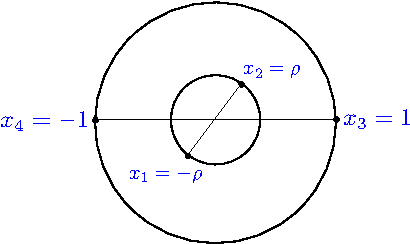
\includegraphics[width=0.55\textwidth]{fig-rho}
\end{center}
\caption{Any four points can be brought to the above configuration using conformal transformations. (Figure from \cite{Hogervorst:2013sma}.)  \label{fig:rho}}
\end{figure}

\begin{exercise}
Show that $\rho=re^{i\theta}$ is related to $z$ via
\be
\label{eq:radialcoordinatedefinition}
\rho = \frac{z}{(1+\sqrt{1-z})^2},\qquad z = \frac{4\rho}{(1+\rho)^2}
\ee
(and similarly for $\bar\rho=r e^{-i\theta}$ and $\bar z$).
\end{exercise}

In radial quantization, this corresponds to placing cylinder operators (\ref{eq:definitionofcylinderop}) at diametrically opposite points $\pm \bn$ and $\pm \bn'$ on $S^{d-1}$, with $\cos\th=\bn\.\bn'$, and with the pairs separated by time $\tau=-\log r$ (figure~\ref{fig:cylinderconfig}).  The conformal block is then
\be
\label{eq:blockintermsofpsi}
 g_{\De,\ell}(u,v) &= \<\psi(\bn)||\cO|e^{-\tau D}|\psi(\bn')\>,
\ee
where we've defined the state\footnote{The factor $2^{\De_\f}=\<\f_\mathrm{cyl.}(0,\bn)\f_\mathrm{cyl.}(0,-\bn)\>^{-1}$ comes from transforming $x_{12}^{-2\De_\f}$ to the cylinder (exercise!).}
\be
|\psi(\bn)\> &\equiv \frac{2^{\De_\f}}{f_{\f\f\cO}}\phi_\mathrm{cyl.}(0,\bn)\phi_\mathrm{cyl.}(0,-\bn)|0\>.
\ee


\begin{figure}
\begin{center}
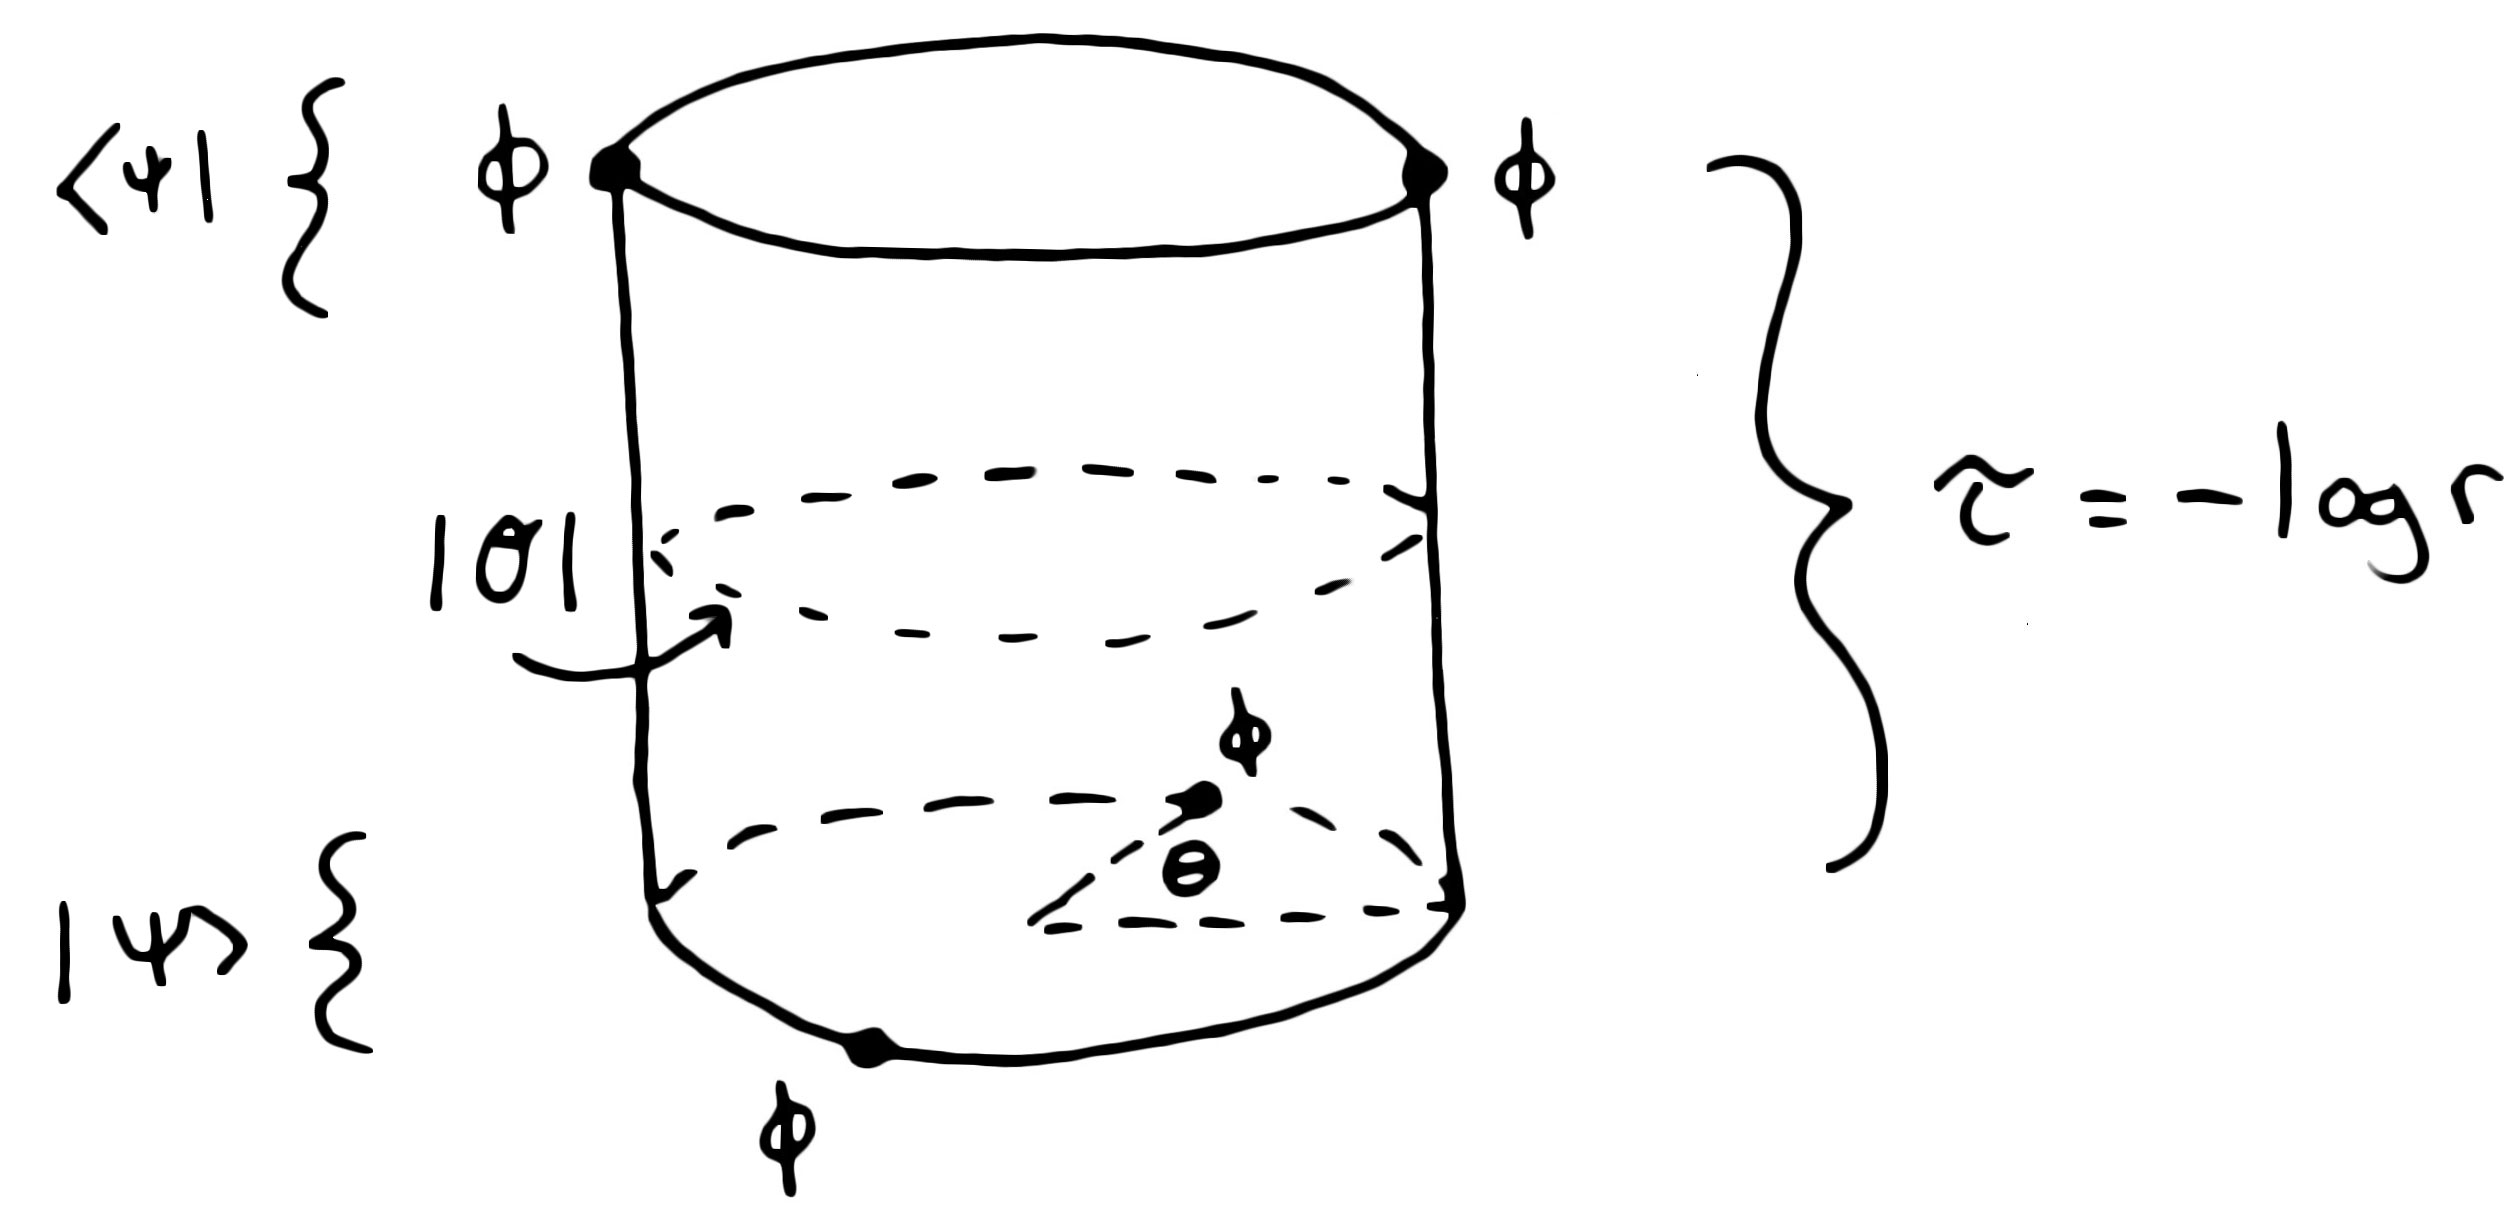
\includegraphics[width=0.75\textwidth]{cylinderconfig.jpg}
\end{center}
\caption{Configuration on the cylinder corresponding to (\ref{eq:blockintermsofpsi}).  \label{fig:cylinderconfig}}
\end{figure}

A descendant $P^{\mu_1}\cdots P^{\mu_n}|\cO\>$ has energy $\De+n$ on the cylinder.  Within the $n$-th energy level, the $\SO(d)$ spins that appear are
\be
\label{eq:rangeofjs}
j \in \{\ell+n,\ell+n-2,\dots,\mathrm{max}(\ell-n,\ell+n\,\,\mathrm{mod}\,\,2)\}.
\ee
Consider a set of descendent states $|n,j\>^{\mu_1\cdots\mu_j}$ with energy $\De+n$ and spin $j$. They contribute
\be
r^{\De+n} \<\psi(\bn)|n,j\>^{\mu_1\cdots\mu_j}{}_{\mu_1\cdots\mu_j}\<n,j|\psi(\bn')\>.
\label{eq:definitespinandenergy}
\ee
By rotational invariance,
\be
\<\psi(\bn)|n,j\>^{\mu_1\cdots\mu_j} &\propto \bn^{\mu_1}\cdots\bn^{\mu_j}-\mathrm{traces}.
\ee
Because $|\psi(\bn)\>=|\psi(-\bn)\>$, $j$ must be even (and thus $n$ is even).
The contraction of two traceless symmetric tensors is a Gegenbauer polynomial,
\be
C_j^{\frac{d-2}{2}}(\bn\cdot\bn') &\propto (\bn^{\mu_1}\cdots\bn^{\mu_j}-\mathrm{traces})(\bn'_{\mu_1}\cdots\bn'_{\mu_j}-\mathrm{traces}),
\ee
so (\ref{eq:definitespinandenergy}) becomes
\be
r^{\De+n} \<\psi(\bn)|n,j\>^{\mu_1\cdots\mu_j}{}_{\mu_1\cdots\mu_j}\<n,j|\psi(\bn')\> &\propto r^{\De+n}C_j^{\frac{d-2}{2}}(\cos\th).
\ee

Summing over descendants, we find
\be
\label{eq:seriesexpansion}
g_{\De,\ell}(u,v) &= \sum_{\substack{n=0,2,\dots \\ j}} B_{n,j}r^{\De+n}C_j^{\frac{d-2}{2}}(\cos\th),%\label{eq:seriesforblock}
\ee
where $j$ ranges over the values in (\ref{eq:rangeofjs}) and $B_{n,j}$ are constants.  
Notice a few properties:
\begin{itemize}
\item The leading term in the $r$-expansion comes from the primary state $|\cO\>$ with $n=0$ and $j=\ell$. This can be used as a boundary condition in the Casimir equation to determine the higher coefficients $B_{n,j}$.
\item The $B_{n,j}$ are positive in a unitary theory because they are given by norms of projections of $|\psi\>$ onto energy and spin eigenstates.
\item The $B_{n,j}$ are rational functions of $\De$.  This follows because the Casimir eigenvalue $\l_{\De,\ell}$ is polynomial in $\De$, or alternatively from the fact that the differential operators $C_a(x,\ptl)$ appearing in the OPE (\ref{eq:scalarscalarOPE}) have a series expansion in $x$ with rational coefficients, see exercise~\ref{exercise:seriesfordiffops}. 
\end{itemize}

\begin{exercise}
Expand $g^{(2d)}_{\De,\ell}(u,v)$ and $g^{(4d)}_{\De,\ell}(u,v)$ to the first few orders in $r$, and check these properties.  Verify that some of the coefficients $B_{n,j}$ become negative when $\De$ violates the unitarity bound.
\end{exercise}

\begin{exercise}
By rewriting in terms of $r,\th$ and using (\ref{eq:seriesexpansion}), show that even spin blocks are invariant under $x_1\leftrightarrow x_2$ or $x_3\leftrightarrow x_4$,
\be
\label{eq:invariantunderonetwo}
g_{\De,\ell}(u,v) &= g_{\De,\ell}\p{\frac{u}{v},\frac 1 v},\qquad(\textrm{$\ell$ even}).
\ee
\end{exercise}

\section{The conformal bootstrap}

\subsection{OPE associativity and crossing symmetry}

We've gotten pretty far using symmetries and basic principles of quantum field theory.  We  classified operators into primaries and descendants. We established the OPE, which determines $n$-point functions as sums of $(n-1)$-point functions,
\be
\label{eq:usingOPEtoreducecorrelator}
\<\cO_1(x_1)\cO_2(x_2)\cdots\cO_n(x_n)\> &= \sum_k C_{12k}(x_{12},\ptl_2)\<\cO_2(x_2)\cdots\cO_n(x_n)\>.\nn\\
\ee
And we showed that the differential operators $C_{ijk}(x,\ptl)$ are determined by conformal symmetry in terms of dimensions $\De_i$, spins, and OPE coefficients $f_{ijk}$. 

Now it's time to implement the last step of the bootstrap program: impose consistency conditions and derive constraints.  Using the OPE, all correlation functions can be written in terms of the ``CFT data" $\De_i,f_{ijk}$.  Now suppose someone hands you a random set of numbers $\De_i,f_{ijk}$.  Does that define a consistent CFT?

\begin{figure}
\begin{center}
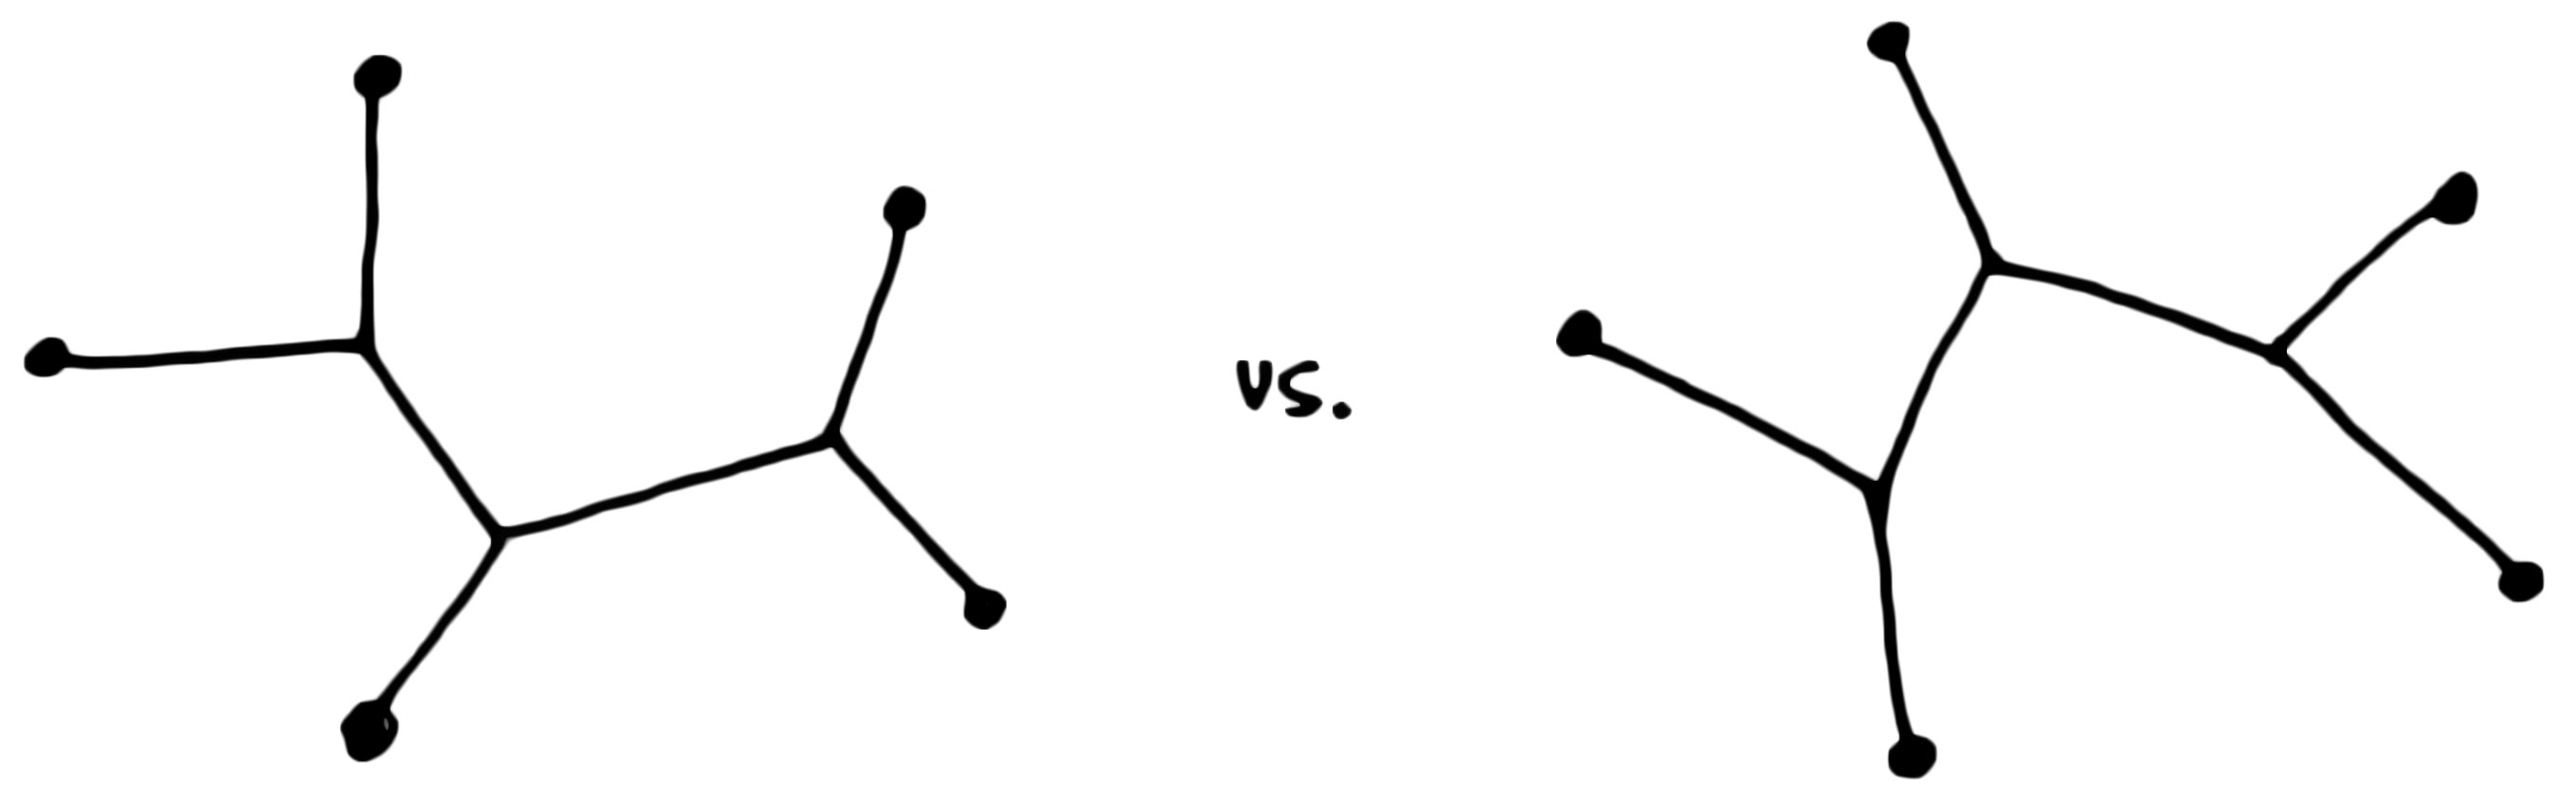
\includegraphics[width=0.9\textwidth]{opedifferentways.jpg}
\end{center}
\caption{Two different ways of evaluating a five-point function using the OPE\@.  Dots represent operators in the correlator, and vertices represent the OPE\@. The two ways differ by a crossing symmetry transformation (\ref{eq:graphicalcrossing}) applied to the left part of the diagram.\label{fig:opedifferentways}}
\end{figure}

The answer is: not always.  By doing the OPE (\ref{eq:usingOPEtoreducecorrelator}) between different pairs of operators in different orders (see figure~\ref{fig:opedifferentways}), we get naively different expressions for the same correlator in terms of CFT data.  These expressions should agree. 
This means the OPE should be associative,
\be
\contraction{}{
\frac 1 2\!\!\!\!\!
\cO_1\cO_2
}{}{\cO_3}
\contraction{}{\cO_1}{}{\cO_2}
\cO_1\cO_2\cO_3
&=
\contraction{}{
\frac 1 2\!\!\!\!\!
\cO_1
}{}{
\contraction{}{\cO_2}{}{\cO_3}
\cO_2\cO_3
}
\contraction{\cO_1}{\cO_2}{}{\cO_3}
\cO_1\cO_2\cO_3,
\ee
or more explicitly,
\be
\label{eq:OPEassociativity}
C_{12i}(x_{12},\ptl_2)C_{i3j}(x_{23},\ptl_3)\cO_j(x_3) &= C_{23i}(x_{23},\ptl_3)C_{1ij}(x_{13},\ptl_3)\cO_j(x_3).\nn\\
\ee
(We suppress spin indices for simplicity.)
Taking the correlator of both sides with a fourth operator $\cO_4(x_4)$ gives the {\it crossing symmetry equation}

\be
\label{eq:graphicalcrossing}
\hspace{-0.4in}
\setlength{\unitlength}{.4in}
\begin{picture}(7,1.7)(0,0.2)
\linethickness{1pt}
\put(1.7,0.4){\line(1,2){0.3}}
\put(1.7,1.6){\line(1,-2){0.3}}
\put(2,1){\line(1,0){0.8}}
\put(2.8,1){\line(1,2){0.3}}
\put(2.8,1){\line(1,-2){0.3}}
\put(1.2,1){\makebox(0,0){$\mathlarger{\sum}_i^{\phantom\cO}$}}
\put(4,1){\makebox(0,0){$=$}}
\put(1.65,1.8){\makebox(0,0){\small $1$}}
\put(1.65,0.2){\makebox(0,0){\small $2$}}
\put(3.15,1.8){\makebox(0,0){\small $4$}}
\put(3.15,0.2){\makebox(0,0){\small $3$}}
\put(5.38,1.8){\makebox(0,0){\small $1$}}
\put(5.38,0.2){\makebox(0,0){\small $2$}}
\put(6.6,1.8){\makebox(0,0){\small $4$}}
\put(6.6,0.2){\makebox(0,0){\small $3$}}
\put(6.3,1){\makebox(0,0){\small $\cO_i$}}
\put(2.4,1.2){\makebox(0,0){\small $\cO_i$}}
\put(5,1){\makebox(0,0){$\mathlarger{\sum}_i^{\phantom\cO}$}}
\put(6,0.6){\line(0,1){0.8}}
\put(5.5,0.35){\line(2,1){0.5}}
\put(6,0.6){\line(2,-1){0.5}}
\put(6,1.38){\line(2,1){0.5}}
\put(5.5,1.65){\line(2,-1){0.5}}
\end{picture}.
\ee
The left-hand side is the conformal block expansion of $\<\cO_1\cO_2\cO_3\cO_4\>$ in the $12\leftrightarrow 34$ channel, while the right-hand side is the expansion in the $14\leftrightarrow 23$ channel.
 
\begin{exercise}
\label{ex:crossingexercise}
Argue that by choosing different operators $\cO_4$ and taking linear combinations of derivatives, one can recover OPE associativity (\ref{eq:OPEassociativity}) from the crossing equation (\ref{eq:graphicalcrossing}). Conclude that crossing symmetry of all four-point functions implies crossing symmetry of all $n$-point functions (i.e.\ that any way of computing an $n$-point function using the OPE gives the same result).
\end{exercise}

%Most of the rest of this course will be devoted to studying its implications for the simplest possible case: a four-point function of identical scalars $\<\f(x_1)\f(x_2)\f(x_3)\f(x_4)\>$.  

\subsubsection{Additional structures and consistency conditions}
\label{sec:additionalstructures}

Let us reflect on the implications of exercise~\ref{ex:crossingexercise}:  A solution to the crossing equations~(\ref{eq:graphicalcrossing}) gives a completely nonperturbative definition of flat-space correlation functions of local operators, without the need for a Lagrangian.  This is most of the way towards a full theory. However, some structures associated with local QFTs are missing, and additional structures might bring new consistency conditions.

Firstly, CFTs can admit extended objects like line operators, surface operators, boundaries, and interfaces. These objects have additional data associated with them, and it's possible to write down OPEs and crossing equations that relate this data to itself and the usual CFT data, see e.g. \cite{Liendo:2012hy,Gaiotto:2013nva}.  It is also interesting to consider correlation functions on manifolds not conformally equivalent to flat space. An example includes the theory at finite temperature (discussed in footnote~\ref{foot:finitetemperature}). This introduces more data, for example the one-point functions of local and extended operators on nontrivial manifolds.\footnote{It is known that this data is not determined by the local operator spectrum.  For example, pure Chern-Simons theory has no local operators at all, but has interesting nonlocal observables that depend on the gauge group and level \cite{Witten:1988hf}.  Also, 4d conformal gauge theories admit different sets of line operators for the same set of local operators \cite{Aharony:2013hda}.} Other interesting constraints come from studying CFTs in Lorentzian signature. Examples include bounds from energy positivity \cite{Hofman:2008ar}, dispersion relations \cite{Komargodski:2011vj,Nachtmann:1973mr,Komargodski:2012ek,Komargodski:2016gci}, and causality \cite{Maldacena:2015waa,Hartman:2015lfa}.

The full set of data and consistency conditions associated with a CFT is not known in general. However, we do have examples of constraints on local operators beyond the OPE and crossing equations. The most famous is modular invariance: the requirement that the partition function of a 2d CFT on the torus $T^2$ be invariant (or covariant) under large diffeomorphisms.  Imposing modular invariance is an additional step that must be performed after solving the crossing equations in 2d CFTs \cite{Moore:1988uz}.\footnote{2d is special because the space of states on a spatial slice $S^1\subset T^2$ is the same as the space of states in radial quantization, and thus modular invariance on $T^2$ directly constrains local operators.  This is not true in $d\geq 3$, so it is not clear how modular invariance on $T^d$ constrains local operators in that case.} We will study modular invariance in more detail in section~\ref{}.
%
\subsection{Crossing symmetry for identical scalars} 
The crossing equation (\ref{eq:graphicalcrossing}) is a powerful but complicated constraint on the CFT data.  
For concreteness, let us write it out for a four-point function of identical real scalars $\<\f(x_1)\f(x_2)\f(x_3)\f(x_4)\>$. We have the conformal block expansion
\be
\<\f(x_1)\f(x_2)\f(x_3)\f(x_4)\> &= \frac{1}{x_{12}^{2\De_\f}x_{34}^{2\De_\f}}\sum_{\cO\in \f\x\f} f_{\f\f\cO}^2 g_{\De,\ell}(u,v),
\label{eq:identicscalarsblockexp}
\ee
where $g_{\De,\ell}(u,v)$ are conformal blocks.  %, and the cross ratios are
%\be
%u = z\bar z = \frac{x_{12}^2 x_{34}^2}{x_{13}^2 x_{24}^2},\qquad v=(1-z)(1-\bar z) =\frac{x_{23}^2 x_{14}^2}{x_{13}^2 x_{24}^2}.
%\ee
By exercise~\ref{exercise:elleven}, $\ell=\ell_\cO$ must be even in order for $\cO$ to appear in an OPE of identical scalars. We have chosen a basis of operators such that the $\cO$'s are real and orthonormal, as in  (\ref{eq:canonicallynormalizedtwopt}).  Unitarity implies that the three-point coefficients $f_{\f\f\cO}$ are real in this basis (section~\ref{sec:realvscomplex}).

Crossing symmetry is equivalent to the statement that the expansion (\ref{eq:identicscalarsblockexp}) should be invariant under permutations of the four points. Invariance under $1\leftrightarrow 3$ or $2\leftrightarrow 4$ implies
\be
\label{eq:crossingeqsummary}
\sum_{\cO\in \f\x\f} f_{\f\f\cO}^2 g_{\De,\ell}(u,v) &= \p{\frac{u}{v}}^{\De_\f} \sum_{\cO\in \f\x\f} f_{\f\f\cO}^2 g_{\De,\ell}(v,u).
\ee
Eq.~(\ref{eq:invariantunderonetwo}) shows that invariance of the four-point function under $1\leftrightarrow 2$ or $3\leftrightarrow 4$ is true block-by-block.  All other permutations can be generated from these. %Thus (\ref{eq:crossingeqsummary}) the only nontrivial condition on the conformal block expansion in this case.

%\end{itemize}

%We know at least two operators present in the $\f\x\f$ OPE: the unit operator and the stress tensor.  Normalizing $\f$ so that $\<\f(x)\f(0)\>=x^{-2\De_\f}$, we have $f_{\f\f\mathbf{1}}=1$.  The stress tensor three-point coefficient is set by Ward identities to be $f_{\f\f T_{\mu\nu}}\propto \De_\f/\sqrt{C_T}$, where $C_T$ is the coefficient of the two-point function of the canonically normalized stress tensor (\ref{eq:twopointfunctionofspinL}).  The factor of $1/\sqrt{C_T}$ relative to (\ref{eq:stresstensorward}) comes from choosing the basis of operators $\cO$ to be orthonormal.

\stoplecture

\subsection{An infinite number of primaries}

As a preview of how the crossing equation works, consider $2$-dimensions. Let us specialize to $z=\bar z$, and study the equation at small $z$. The leading term on the left-hand side is the unit operator, which has conformal block given by
\be
g_{\De=0,\ell=0}(u,v) &= 1.
\ee
On the right-hand side, expanding the blocks at small $z$, we find
\be
g_{\De,\ell}^{(2d)}(v,u)|_{z=\bar z} &= 2 k_{\De+\ell}(1-z) k_{\De-\ell}(1-z)\nn\\
& \sim \log^2 z + \dots,
\ee
where $\dots$ represents less singular terms as $z\to 0$.

Thus, the structure of the crossing equation is
\be
1 &\sim z^{2\De_\f} \sum_\cO (\log^2 z + \dots).
\ee
This immediately looks like a contradiction because $\lim_{z\to 0} z^{2\De_\f} \log^2 z = 0$, but the left-hand side is nonzero.

The problem is that the sum $\sum_\cO$ does not commute with the small-$z$ expansion of the blocks. A toy model for what's happening is the expression
\be
\lim_{z\to 0} \sum_{n=0}^\oo z e^{-n z}.
\ee
Taking the limit inside the sum, we get 0 term-by-term. However, this is incorrect. We must perform the sum first, giving $\lim_{z\to 0} \frac{z}{1-e^{-z}}=1$. The key point is that while $e^{-nz}$ is regular at $z=0$, an infinite sum of terms of the form $e^{-nz}$ can become singular at $z=0$.

A similar phenomenon occurs in the crossing equation. Although each individual block on the right-hand side has at most a $\log^2 z$ singularity as $z\to 0$, an infinite sum of blocks can give an enhanced singularity of the form $z^{-2\De_\f}$, which cancels the $z^{2\De_\f}$ to give $1$.

We conclude that any CFT must have an infinite number of primary operators, since this is necessary for consistency of the crossing equation.

One of our main goals for the rest of the course will be to study the crossing equations and find solutions if possible. 2-dimensional CFTs possess extra symmetries that will allow us to make significant progress in this direction. We will specialize to 2 dimensions in section~\ref{sec:twod}. Before we do so, there are a few more results to discuss in higher dimensions.

\section{Ward identities}

\subsection{Spin-$1$ current}

Most of the three-point coefficients $f_{ijk}$ are unknown a-priori. However, some coefficients involving conserved currents are fixed by symmetries.
For example, let $J^\mu$ be a conserved primary spin-1 operator. By integrating $J^\mu$ over a surface, we can form the conserved charge
\be
Q(\Sigma) &\equiv i\int_\Sigma dS_\mu J^\mu.
\ee
(The factor of $i$ is so that $Q$ is Hermitian when $\Sigma$ is a spatial slice.)  Unitarity implies (\ref{eq:thmaboutconserved}) that $J$ has dimension $d-1$, so $Q$ is dimensionless. Note that $Q$ commutes with conformal transformations.

Suppose $\f(x)$ is a complex scalar with charge $q$ under $Q$,
\be
[Q,\f(x)] &= q \f(x).
\ee
Recall that the three-point function $\<\f^* \f J\>$ is fixed by conformal symmetry up to a coefficient (equation~(\ref{eq:scalarscalarspinL})):
\be
\label{eq:threeptcurrent}
\<\f^*(x_1) \f(x_2) J^\mu(x_3)\> &= \frac{f_{\f^*\f J}}{x_{12}^{2\De_\f-d+2} x_{23}^{d-2} x_{31}^{d-2}}\p{\frac{x_{13}^\mu}{x_{13}^2} - \frac{x_{23}^\mu}{x_{23}^2}}.
\ee
Integrating $x_3$ over a surface $\Sigma$ surrounding $x_2$, we find
\be
\label{eq:wardidentitywefind}
i\int_\Sigma dS_\mu(x_3) \<\f^*(x_1) \f(x_2) J^\mu(x_3)\>
&=
\<\f^*(x_1)Q(\Sigma) \f(x_2) \>\nn\\
 &= q\<\f^*(x_1) \f(x_2)\>.
\ee
Plugging in (\ref{eq:threeptcurrent}), we see that $f_{\f\f J}$ is fixed in terms of $q$.

It is useful to specialize to the configuration\footnote{Recall that $\f^*(\oo) \equiv \lim_{L\to \oo} L^{2\De_\f} \f^*(Le)$, where $e$ is a unit vector.}
\be
\label{eq:specialkinematics}
\<\f^*(\oo) J^\mu(x) \f(0)\> &= f_{\f^* \f J} \frac{x^\mu}{x^d}.
\ee
In this configuration, the Ward identity (\ref{eq:wardidentitywefind}) becomes
\be
\label{eq:chargeintegral}
q &= i\int_\Sigma dS_\mu(x) \frac{f_{\f^*\f J} x^\mu }{x^{d}} = i S_d f_{\f^*\f J},
\ee
where $S_d=\frac{2\pi^{d/2}}{\Gamma(d/2)}$ is the volume of the unit sphere in $d$-dimensions. The fact that the integral in (\ref{eq:chargeintegral}) only depends on the topological class of $\Sigma$ is simply Gauss' law from electrostatics.

%\begin{exercise}
%Derive $q=iS_d f_{\f^* \f J}$ directly from (\ref{eq:wardidentitywefind}) without specializing the positions of the operators.
%\end{exercise}

We can summarize this result by writing the $\f$ term in the $J\x\f$ OPE:
\be
J^\mu(x) \f(0) &= -\frac{i}{S_d}q \frac{x^\mu}{x^d} \f(0) + \dots.
\ee
Here ``$\dots$" represents descendants of $\f$ and other conformal multiplets. Taking the correlator of both sides with $\f^*(\oo)$, we get back to (\ref{eq:specialkinematics}). Integrating $J^\mu$ around a sphere $\Sigma$ centered at $\f$ gives $Q(\Sigma)\f(0)=q\f(0)$.

More generally, suppose $\f_i$ are scalar operators. The commutator $[Q,\f_i]$ must be a primary scalar, since $Q$ commutes with the conformal generators. Thus, we can write
\be
\label{eq:generalizedQ}
[Q,\f_i(x)] &= t_i{}^j \f_j(x),
\ee
for some matrix $t_i{}^j$. Note that $t_i{}^j$ can only be nonzero if $\De_i=\De_j$, by dimensional analysis (more formally, by acting on both sides of (\ref{eq:generalizedQ}) with $D$).
Repeating the above computation, we find
\be
\label{eq:jope}
J^\mu(x) \f_i(0) &= -\frac{i}{S_d} t_i{}^j \frac{x^\mu}{x^d} \f_j(0) + \dots.
\ee
We can also see here that $\f_j$ must have the same dimension as $\f_i$. Otherwise, the $x$-dependence in (\ref{eq:jope}) would be $x^\mu x^{\De_j-\De_i-d}$, which is not conserved.

In general, if $\cO_i,\cO_j$ have spin, there can be multiple three-point structures for $\<\cO_i \cO_j J\>$. One of these three-point structures will be fixed by the Ward-identity, and the others will be unconstrained. For example, given a collection of currents $J_\mu^a$ generating a nonabelian symmetry with structure constants $f^{abc}$, the three-point function will have the form
\be
\<J^a J^b J^c\> &= f^{abc}\x(\textrm{Ward-identity structure}) + \textrm{other structures}.
\ee

\subsection{The stress-tensor}
\label{sec:stresstensorward}

Some OPE coefficients of the stress-tensor are also fixed by Ward identities in a similar way. Again, there is only a single conformally-invariant structure for a three-point function $\<\f_i \f_j T^{\mu\nu}\>$. The integral of $T^{\mu\nu}$ gives the conformal charges, so $f_{ij T}$ must be proportional to $C_{ij}=\<\f_i \f_j\>$.

To compute the constant of proportionality, let us jump straight to the OPE
\be
T^{\mu\nu}(x) \f_i(0) &= f_{T i}{}^{j} \frac{x^\mu x^\nu - \tfrac{1}{d} x^2 \de^{\mu\nu}}{x^{d+2}} \f_j(0) + \dots,
\ee
where $f_{Ti}{}^k C_{kj}=f_{Tij}$. One can derive this expression by taking the correlator of both sides with another scalar and using (\ref{eq:scalarscalarspinL}). However, a shortcut is to use dimensional analysis and tracelessness of $T^{\mu\nu}$ to fix the form that the OPE can take. One can check that the result is automatically conserved (away from the origin).

Note that the dilatation operator is given by
\be
D(\Sigma) &= - \int_\Sigma dS_\mu x_\nu T^{\mu\nu}.
\ee
Applying this above, we find
\be
\De_i \f_i(0) &= D(\Sigma) \f_i(0) = -f_{Ti}{}^j \int dS_\mu \frac{d-1}{d}\frac{x^\mu}{x^d} \f_j(0) \nn\\
&= -\frac{d-1}{d}S_d f_{Ti}{}^j \f_j(0).
\ee
Thus, we have the OPE
\be
\label{eq:tope}
T^{\mu\nu}(x) \f_i(0) &= - \frac{d\De_i}{S_d(d-1)} \frac{x^\mu x^\nu - \tfrac{1}{d} x^2 \de^{\mu\nu}}{x^{d+2}} \f_i(0) + \dots
\ee

We fixed the OPE coefficient $f_{\f_i \f_j T}$ using just the dilatation operator. But what about the other conformal generators? The most interesting case is $P^\mu$.
\begin{exercise}
Using conservation and tracelessness of $T^{\mu\nu}$, show that the term proportional to $\ptl \f_i(0)$ in the $T^{\mu\nu}(x)\f_i(0)$ OPE is given by
\be
\label{eq:tderivativeterm}
T^{\mu\nu}(x) \f_i(0) &= (\ref{eq:tope}) + A \p{\frac{x^\mu\ptl^\nu+x^\nu\ptl^\mu-\de^{\mu\nu}x\.\ptl}{x^d}+(d-2)\frac{x^\mu x^\nu}{x^{d+2}}x\.\ptl} \f_i(0) \nn\\
& \quad + \dots
\ee
for some constant $A$. In general, the contribution of $\f_i$ to the OPE is
\be
\label{eq:generalopeTphi}
T^{\mu\nu}(x_1)\f_i(x_2) &= C^{\mu\nu}(x_{12},\ptl_2) \f_i(x_2) + \textrm{other multiplets},
\ee
where $C^{\mu\nu}(x,\ptl)$ is a differential operator. By taking the correlator of both sides of (\ref{eq:generalopeTphi}) with $\f_i(x_3)$ and using the known form of a conformally-invariant three-point function (\ref{eq:scalarscalarspinL}), show that
\be
A &=\frac{2}{\De_i} f_{Ti}{}^j = -\frac{d}{2S_d(d-1)}.
\ee
Check that this is precisely the value needed to give the Ward identity for momentum
\be
[P^\mu,\f_i(0)] &= -\int_\Sigma dS_\nu(x) T^{\mu\nu}(x) \f_i(0) = \ptl^\mu \f_i(0),
\ee
\end{exercise}

Once we have fixed the coefficient $f_{Ti}{}^j$ using the dilatation Ward identity, we will find that all other Ward identities are automatically satisfied. The situation is different for non-scalar operators $\cO_i$. In this case, there can be multiple conformally-invariant structures for the three-point function $\<\cO_j \cO_i T^{\mu\nu}\>$. In general, Ward identities for both $D$ and $M_{\mu\nu}$ can give nontrivial constraints on these structures. The Ward identities for $P$ and $K$ will follow as a consequence.


\stoplecture


%
%We fixed the OPE coefficient $f_{\f_i \f_j T}$ using just the dilatation operator. But what about the other conformal generators? The most interesting case is $P^\mu$. Let us check how its Ward identity is satisfied.
%As usual, the coefficients of all descendent operators $\ptl\cdots\ptl \f_i$ are fixed by conformal invariance in terms of the same OPE coefficient
%\be
%T^{\mu\nu}(x_1) \f_i(x_2) &= - \frac{d\De_i}{S_d(d-1)}C^{\mu\nu}(x_{12},\ptl_2) \f_i(x_2) + \dots
%\ee
%By a similar computation to exercise~\ref{}, we find
%\be
%C^{\mu\nu}(x,\ptl) &= \frac{x^\mu x^\nu - \tfrac{1}{d} x^2 \de^{\mu\nu}}{x^{d+2}}\p{1+\frac{d}{\De_i} x\.\ptl + \dots}
%\ee
%Let us include this next term in the OPE
%\be
%T^{\mu\nu}(x) \f_i(0) &= - \frac{d\De_i}{S_d(d-1)} \frac{x^\mu x^\nu - \tfrac{1}{d} x^2 \de^{\mu\nu}}{x^{d+2}} \p{\f_i(0)+\frac{d}{\De_i} x\.\ptl \f_i(0) + \dots} \nn\\
%&\qquad + \dots
%\ee
%The momentum operator is given by
%\be
%P^\mu = -\int_\Sigma dS_\nu T^{\mu\nu}.
%\ee
%Applying this to the first two terms above, with $\Sigma=S^{d-1}$ centered at the origin, we find the following integrals
%\be
%-\int_{S^{d-1}} dS_\nu \frac{x^\mu x^\nu - \tfrac 1 d x^2 \de_{\mu\nu}}{x^{d+2}} &= 0\nn\\
%-\int_{S^{d-1}} dS_\nu \frac{x^\mu x^\nu - \tfrac 1 d x^2 \de_{\mu\nu}}{x^{d+2}}x_\rho &= -\frac{d-1}{d^2} S_d \de^\mu_\rho.
%\ee
%Thus, we recover
%\be
%[P^\mu,\f_i(0)] &= \ptl^\mu \f_i(0).
%\ee


\subsection{Two-point functions of conserved currents}
\label{sec:twoptconserved}

In our discussion of conformal blocks, we used a convention that all two-point functions are normalized (\ref{eq:canonicallynormalizedtwopt}) as,
\be
\label{eq:standardtwopt}
\<\cO^{a}(x) \cO^{b}(0)\> &= \frac{I^{ab}(x)}{x^{2\De}},
\ee
where $I^{ab}(x)$ is a standard tensor. For example, for a traceless symmetric tensor
\be
I^{\mu_1\mu_2}{}_{\nu_1\nu_2}(x) &= I^{(\mu_1}{}_{\nu_1}(x) \cdots I^{\mu_\ell)}{}_{\nu_\ell}(x)-\textrm{traces}.
\ee
However, conserved currents and the stress tensor come with a canonical normalization given by demanding that their integrals give the correct charges. Alternatively, we can imagine computing $J^\mu,T^{\mu\nu}$ using the Noether procedure, and this does not give us the freedom to rescale them. The OPEs (\ref{eq:jope}) and (\ref{eq:tope}) are written using this canonical normalization.

In the canonical normalization, we have
\be
\<J^\mu(x)J_\nu(0)\> &= C_J \frac{I^{\mu}{}_{\nu}(x)}{x^{2(d-1)}} \nn\\
\<T^{\mu\nu}(x) T_{\rho\s}(0)\> &= 2C_T \frac{I^{(\mu}{}_{\rho}(x) I^{\nu)}{}_{\s}(x)-\frac{1}{d} \de^{\mu\nu}\de_{\rho\s}}{x^{2d}}.
\ee
The two-point coefficients $C_J, C_T$ are interesting physical observables. Note that they must be positive in a unitary theory. To see this, we can use (\ref{eq:bpznormprim}) to compute
\be
0 &\leq \sum_\mu ||J^\mu\>|^2 = \<J_\mu|J^\mu\> = d C_J \nn\\
0 &\leq \sum_{\mu,\nu} ||T^{\mu\nu}\>|^2 = \<T_{\mu\nu}|T^{\mu\nu}\> = (d^2+d-2)C_T.
\ee
If $C_J$ or $C_T$ vanished, the corresponding state $|J^\mu\>$ or $|T^{\mu\nu}\>$ would have to vanish, which would mean the operators $J^\mu$ or $T^{\mu\nu}$ vanished identically, a contradiction.

When an operator has a non-standard two-point function $\<\cO(x) \cO(0)\> = C_\cO I(x)/x^{2\De}$, the corresponding coefficients in the conformal block expansion get modified according to
\be
f_{\f\f\cO}^2 &\to \frac{f_{\f\f\cO}^2}{C_\cO}.
\ee
For example, the coefficient of the stress-tensor in the conformal block expansion of $\<\f\f\f\f\>$ is proportional to
\be
\frac{f_{\f\f T}^2}{C_T} &\propto \frac{\De_\f^2}{C_T}.
\ee

\section[2 dimensions]{2 dimensions\footnote{Sources for this section: Polchinski \cite{}.}}
\label{sec:twod}

\subsection{Conventions}

We now specialize to $2$-dimensional CFTs and discuss the extra structure that is present there. It is useful to adopt complex coordinates
\be
z &= x^1 + i x^2,\quad \bar z= x^1 - i x^2.
\ee
A vector $v^\mu$ has components
\be
v^z = v^1 + i v^2,\quad v^{\bar z} = v^1 - iv^2,\quad v_z=\frac 1 2 (v^1 - i v^2),\quad v_{\bar z} = \frac 1 2 (v^1 + i v^2).
\ee
These components are raised and lowered using the metric
\be
g_{z\bar z} = g_{\bar z z} = \tfrac 1 2, \quad g_{zz}=g_{\bar z\bar z}=0,\quad g^{z\bar z} = g^{\bar z z} =2,\quad g^{zz} =g^{\bar z \bar z} = 0.
\ee
We also define
\be
\ptl \equiv \ptl_z=\tfrac1 2(\ptl_1-i\ptl_2)=\tfrac 1 2 \ptl^{\bar z},\qquad \bar \ptl \equiv \ptl_{\bar z} = \tfrac 1 2 (\ptl_1+i\ptl_2) = \tfrac 1 2 \ptl^z.
\ee

\subsection{The stress tensor and conformal charges}

Let us study the conditions on the stress-tensor in these coordinates. Tracelessness is the statement that
\be
\label{eq:tracelessness2d}
T_{z\bar z} = 0.
\ee
The conservation condition then implies
\be
\label{eq:conservation2d}
0 &= \ptl^{\bar z} T_{\bar z \bar z} + \ptl^z T_{z\bar z} = \tfrac 1 2\ptl T_{\bar z \bar z} \nn\\
0 &= \ptl^z T_{zz} + \ptl^{\bar z} T_{\bar z z} = \tfrac 1 2\bar\ptl T_{zz}.
\ee
In other words, $T_{zz}$ is holomorphic and $T_{\bar z \bar z}$ is anti-holomorphic. Because $T_{zz}$ is holomorphic, it is traditional to write it as a function of $z$ alone, and similarly for $T_{\bar z\bar z}$,
\be
T_{zz}(z,\bar z) &= T(z) \nn\\
T_{\bar z \bar z}(z,\bar z) &= \bar T(\bar z).
\ee

As usual, the conditions (\ref{eq:tracelessness2d}) and (\ref{eq:conservation2d}) hold as operator equations, which means they are true at separated points, but can be violated by contact terms when $T^{\mu\nu}(x)$ becomes coincident with other operators. This means that correlators of $T(z)$ are only constrained to be holomorphic at separated points. For example, they can have poles at the locations of other insertions
\be
\<T(z) \cO(z_0,\bar z_0)\cdots\> &\sim \frac{1}{(z-z_0)^2} + \dots.
\ee

In 2 dimensions, it is conventional to include a factor of $-2\pi$ in the definition of $T^{\mu\nu}$,
\be
\label{eq:defstresstwod}
\<T^{\mu\nu}\cdots\>_g &= -2\pi \frac{2}{\sqrt g}\frac{\de}{\de g^{\mu\nu}}\<\cdots\>_g\qquad (\textrm{$2$-dimensions})
\ee
The conformal charges are then given by
\be
Q_\e(\Sigma) &= \frac{1}{2\pi} \int_\Sigma dS^\mu \e^\nu(x) T_{\mu\nu}(x)\qquad (\textrm{$2$-dimensions}),
\ee
where $\e^\mu$ is a conformal Killing vector.

Recall that the solutions to the conformal Killing equation in 2d are given by (\ref{eq:killingvectwod})
\be
\e^\mu \ptl_\mu &= \e(z) \ptl + \bar\e(\bar z) \bar\ptl,
\ee
where $\e(z)$ is purely holomorphic and $\bar\e(\bar z)$ is purely anti-holomorphic.
In terms of $\e,\bar \e$, the charges become
\be
\label{eq:definitionofchargetwod}
Q_\e(\Sigma) %&= \frac{1}{2\pi} \int_\Sigma dS^\mu \e^\nu(x) T_{\mu\nu}(x) \nn\\
&= \frac{1}{2\pi i}\oint_\Sigma dz\, \e(z) T(z) - \frac{1}{2\pi i} \oint_\Sigma d\bar z\, \bar \e(\bar z) \bar T(\bar z)
\ee
The space of globally-defined holomorphic vector fields on $S^2$ is only three-dimensional. However, to define topological surface operators, we only need holomorphicity in a neighborhood of the curve $\Sigma$ where the charges are defined. Thus, we can allow $\e(z)$ and $\bar\e(\bar z)$ to have poles. The charges $Q_\e(\Sigma)$ will be topological away from the poles.

It is conventional to define a basis of conformal Killing vectors given by
\be
\ell_m &= z^{m+1} \ptl,\quad \bar \ell_m=\bar z^{m+1} \bar\ptl.
\ee
As vector-fields, they satisfy the Witt algebra
\be
\label{eq:wittalgebra}
[\ell_m,\ell_n]=-(m-n)\ell_{m+n}
\ee
and similarly for $\bar\ell_m$. The corresponding charges are
\be
L_m(\Sigma) &= Q_{\ell_m}(\Sigma) = \frac{1}{2\pi i}\oint_\Sigma z^{m+1} T(z) \nn\\
\bar L_m(\Sigma) &= Q_{\bar\ell_m}(\Sigma) = -\frac 1 {2\pi i} \oint_\Sigma \bar z^{m+1} \bar T(\bar z).
\ee

\begin{exercise}
Show that the $L_m,\bar L_m$ for $m=-1,0,1$ are related to the usual generators of $\SO(d+1,1)=\SO(3,1)$ by
\be
\label{eq:relationtoglobalcharges}
L_{-1} = P_z,\quad L_0 = \tfrac1 2 (D+i M_{12}),\quad L_{1}= K_{\bar z} \nn\\
\bar L_{-1} = P_{\bar z},\quad \bar L_0 = \tfrac 1 2 (D-i M_{12}),\quad \bar L_1=K_z.
\ee
Show that they generate the algebra $\mathrm{SL}(2,\R)\x \mathrm{SL}(2,\R)$:
\be
[L_0,L_1]=-L_1,\quad [L_0,L_{-1}]=L_{-1},\quad [L_1,L_{-1}]=2L_0 \nn\\
[\bar L_0,\bar L_1]=-\bar L_1,\quad [\bar L_0,\bar L_{-1}]=\bar L_{-1},\quad [\bar L_1,\bar L_{-1}]=2\bar L_0
\ee
with all other commutators vanishing.
\end{exercise}
The fact that of $\SO(3,1)\cong \mathrm{SL}(2,\R)\x \mathrm{SL}(2,\R)$ as complexified Lie algebras is a familiar group theory fact.

We call $L_{-1,0,1},\bar L_{-1,0,1}$ the ``global" conformal charges because they come from conformal Killing vectors that are globally-defined on the sphere $S^2$. This is in contrast to the charges $L_m,\bar L_m$ for $m\notin\{-1,0,1\}$, which come from conformal Killing vectors with poles (either at zero or infinity).

\subsubsection{BPZ conjugation}

Recall from section~\ref{sec:reflposcyl} that the BPZ conjugate of $Q_\e$ is $Q_\e^\dag = Q_{-I\e^* I^{-1}}$, where $I$ acts on functions by $(I f)(x)=f(I(x))$. In our coordinates, an inversion acts as $I(z,\bar z) = (1/\bar z, 1/z)$, so we have
\be
(-I \ell_m^* I)f(z,\bar z) &= \left.-(\bar z^{m+1}\bar\ptl) f\p{\frac 1 {\bar z},\frac 1 { z}}
\right|_{(z,\bar z) \to \p{\frac 1 {\bar z},\frac 1 { z}}} \nn\\
%&= - \left.\bar z^{m+1} \bar\ptl f\p{\frac 1 {\bar z},\frac 1 { z}}
%\right|_{(z,\bar z) \to \p{\frac 1 {\bar z},\frac 1 { z}}}\nn\\
&= \left.\bar z^{m-1} f^{(1,0)}\p{\frac 1 {\bar z},\frac 1 { z}}
\right|_{(z,\bar z) \to \p{\frac 1 {\bar z},\frac 1 { z}}}\nn\\
&=\ell_{-m} f(z,\bar z).
\ee
Thus, we have
\be
L_m^\dag = L_{-m},\quad \bar L_m^\dag = \bar L_{-m}.
\ee
This is easy to verify for the global charges from (\ref{eq:relationtoglobalcharges}).

Essentially, complex conjugation exchanges $z$ and $\bar z$, but reflection exchanges them back.
As another example, consider a local operator $\cO_{\mu_1\cdots\mu_J}(z,\bar z)$ satisfying the reality condition (\ref{eq:reflectionforhermitianconjugation}). Hermitian conjugation maps $z,\bar z$ components to themselves, for example
\be
\cO_{z\cdots z}^\dag(z,\bar z) &= \cO_{z \cdots z}(\bar z,z).
\ee
This is necessary for a purely holomorphic operator to have a nonvanishing two-point function consistent with unitarity,
\be
\p{\frac{c}{z_{12}^4}}^* = \<0|T_{zz}(z_1)T_{zz}(z_2)|0\>^\dag = \<0|T_{zz}(\bar z_2) T_{zz}(\bar z_1)|0\> = \frac{c}{\bar z_{12}^4}.
\ee


\subsection{The Virasoro algebra}

In exercise~(\ref{exercise:primarytransofmationfort}), we argued that in $d\geq 3$
\be
\label{eq:higherdimQT}
[Q_\z,T^{\mu\nu}] &= \z^\rho \ptl_\rho T^{\mu\nu} + (\ptl\.\z)T^{\mu\nu} - \ptl_\rho \z^\mu T^{\rho \nu} + \ptl^\nu \z_\rho T^{\rho \mu} \quad (d\geq 3).
\ee
The form of this expression is fixed by dimensional analysis, conservation and tracelessness of $T^{\mu\nu}$, and the Ward identity for momentum. In retrospect, we can see that it is equivalent to the condition that $T^{\mu\nu}$ transforms like a primary under the global conformal algebra $\SO(3,1)$.

In $d=2$ dimensions, it is possible to write two additional terms proportional to the unit operator that are consistent with these conditions (exercise~\ref{exercise:virasoro}):
\be
\label{eq:extraterm}
[Q_\z,T^{\mu\nu}] &= (\ref{eq:higherdimQT}) + a\,\ptl^\mu \ptl^\nu \ptl\.\z + b\,\ptl^\mu \ptl^\nu \ptl\.\tl\z
\ee
where 
\be
\tl \z_\mu = \e_{\mu\nu} \z^\nu
\ee
with $\e_{\mu\nu}$ the 2-dimensional $\e$-symbol. Here $a,b$ are constants. Note that tracelessness and conservation are implied by $\ptl^2 (\ptl\.\z)=\ptl^2 (\ptl\.\tl\z)=0$, which is a consequence of the conformal Killing equation  (equation~(\ref{eq:termneededforvirasoro})). The extra term in (\ref{eq:extraterm}) does not affect the global generators because the corresponding vector fields are at most quadratic polynomials in $x$.

In holomorphic coordinates, (\ref{eq:extraterm}) becomes
\be
[Q_\z,T(z)] &= (\ref{eq:higherdimQT}) + \frac{c}{12}\ptl^3 \z(z), \nn\\
[Q_\z,\bar T(\bar z)] &= (\ref{eq:higherdimQT}) + \frac{\bar c}{12}\bar \ptl^3 \bar\z(\bar z),
\ee
where we have defined
\be
c = 12(a + ib),\quad \bar c = 12(a - i b).
\ee
(The factors of $12$ are for later convenience.)
Plugging into (\ref{eq:definitionofchargetwod}), we find a modification of the algebra of charges
\be
\label{eq:virasoronice}
[Q_{\z},Q_{\xi}] &= Q_{-[\z,\xi]} + \frac c {24\pi i} \oint_\Sigma dz\, \xi(z) \ptl^3 \z(z) - \frac{\bar c}{24\pi i} \oint_\Sigma d\bar z\, \bar\xi(\bar z)\bar\ptl^3 \bar \z(\bar z),
\ee
where the contour $\Sigma$ is the same as the one used to define $Q_\xi$.
Let us consider charges defined on a circle surrounding the origin. Applied to $L_m,\bar L_m$, (\ref{eq:virasoronice}) becomes
\be
\label{eq:virasoroalgebra}
[L_m,L_n] &= (m-n)L_{m+n} + \frac{c}{12} (m^3-m) \de_{m,-n}.
\ee
The $\bar L_m$ satisfy the same algebra with $\bar c$ instead of $c$. We call $L_m$ the ``left-moving" Virasoro algebra and $\bar L_m$ the ``right-moving" Virasoro algebra.

The commutation relations (\ref{eq:virasoroalgebra}) define the so-called Virasoro algebra. The constant $c$ is called the ``central charge." The Virasoro algebra is a nontrivial central extension of the Witt algebra (\ref{eq:wittalgebra}). ``Central" refers to the fact that the term in (\ref{eq:virasoroalgebra}) proportional to $c$ commutes with all the generators --- i.e.\ it is in the center of the algebra.

\subsection{Determining the central charge}
\label{sec:determinec}

We have seen that a central term is consistent with basic properties of the stress tensor. However, does it actually need to be there? We can find out by computing it. Let us study the vacuum expectation value of the simplest expression containing $c$. This is
\be
\frac c 2 = \<[L_2,L_{-2}]\> = \left\<\frac{1}{2\pi i} \oint_{C_1} dz_1 z_1^3 T(z_1) \frac{1}{2\pi i} \oint_{C_2} dz_2 z_2^{-1} T(z_2)\right\> - (C_2 \leftrightarrow C_1). \nn\\
\ee
Here $C_1,C_2$ are circles surrounding the origin, with $C_1$ outside $C_2$. Because there is no singularity in the integrand when $z_2$ is near the origin and $T(z_2)$ is holomorphic, the $z_2$-integral just gives $T(0)$ by Cauchy's theorem. The term with $C_2\leftrightarrow C_1$ vanishes because $z_1^3 T(z_1)$ is holomorphic inside $C_2$. (Recall that $T(z)$ can fail to be holomorphic when it coincides with other operator insertions, but in this case the other $T$ is outside $C_2$.) Thus, we find
\be
\frac c 2 &= \frac{1}{2\pi i} \oint_{C_1} dz_1 z_1^3\< T(z_1) T(0) \>
\ee

We saw in section~\ref{sec:twoptconserved} that
\be
\label{eq:twoptstresstwod}
\<T_{\mu\nu}(x)T_{\rho\s}(0)\> &= 2C_T \frac{\tfrac 1 2 (I_{\mu\rho}(x) I_{\nu\s}(x) + I_{\mu\s}(x) I_{\nu\rho}(x)) -  \tfrac{1}{d}\de_{\mu\nu} \de_{\rho\s}}{x^4},
\ee
where $C_T$ is positive in a unitary theory. In 2d, this expression actually assumes parity-invariance, as we discuss below, but let us continue on for now.
\begin{exercise}
Show that in holomorphic coordinates, (\ref{eq:twoptstresstwod}) becomes
\be
\label{eq:twodstressholo}
\<T(z)T(0)\> &= \frac{C_T}{2 z^4}.
\ee
\end{exercise}
We could have alternatively derived (\ref{eq:twodstressholo}) just using dimensional analysis and holomorphicity. Plugging (\ref{eq:twodstressholo}) into (\ref{eq:twoptstresstwod}), we find
\be
c &= C_T.
\ee
Thus, $c$ is related to the two-point function of stress tensors, and it is nonzero and positive in any unitary theory.

If we allow ourselves to use the 2d $\e$-symbol, then there is actually an additional allowed tensor structure for $\<T_{\mu\nu}(x)T_{\rho\s}(0)\>$.\footnote{Exercise: find it!} Previously in section~\ref{sec:twoptsection} we proved that operators in an irreducible representation of $\SO(d)$ have a unique two-point structure. This is not a contradiction because the spin-$\ell$ representation in 2d is actually {\it reducible}. Specifically, $\SO(2)=U(1)$, and the spin-$\ell$ representation splits into two 1-dimensional irreps of $U(1)$ with charges $s=\pm \ell$. In the case of the stress tensor, these irreps are precisely described by $T(z)=T_{zz}(z)$ and $\bar T(\bar z) = T_{\bar z\bar z}(\bar z)$ --- they don't mix with each other under $\SO(2)$ rotations. Thus, it is possible to write two separate two-point structures\footnote{Note that the charge $\ell$ representation under $\SO(2)=U(1)$ is isomorphic to its dual-reflected representation, which allows these two-point functions to be nonvanishing.}
\be
\<T(z)T(0)\> = \frac{c}{2z^4},\quad \<\bar T(\bar z) \bar T(0)\> = \frac{\bar c}{2\bar z^4},
\ee
where $c,\bar c$ can be different. By a similar calculation to the above, we find that $\bar c$ is the central charge for the antiholomorphic Virasoro algebra.

Unitarity implies that $c$ and $\bar c$ are each nonnegative:
\be
\frac c 2 &= \<0|[L_{2},L_{-2}]|0\> = \<0|L_2 L_{-2}|0\> = |L_{-2}|0\>|^2
\ee
(and similarly for $\bar c$). In a parity-invariant theory, we would have $c=\bar c$.


\stoplecture


\subsection{Virasoro multiplets}
\label{sec:virasorormult}

One of the commutation relations of the Virasoro algebra is
\be
[L_0,L_m] &= -m L_m.
\ee
Thus, the generators $L_m$ with $m>0$ are {\it lowering} operators for $L_0$ and the generators with $m<0$ are {\it raising} operators.

Recall that $L_0 = \tfrac 1 2(D+i M_{12})$. Acting on an operator with spin $\ell$, its eigenvalues are given by $\tfrac 1 2 (\De\pm \ell)$. The unitarity bounds (\ref{eq:unitaritysummary}) imply that this is positive. We can also re-derive the unitarity bounds using the fact that $L_{-1}^\dag = P_z^\dag = K_{\bar z} = L_1$, so
\be
0 \leq |L_{-1} |\cO\>|^2 = \<\cO|L_1 L_{-1}|\cO\> = 2\<\cO|L_0|\cO\>,
\ee
where $|\cO\>$ is a primary state with respect to $\SL(2,\R)$ (i.e.\ it is killed by $L_1=K_{\bar z}$). Thus, $L_0$ has positive eigenvalues in any $\SL(2,\R)$-primary state, and consequently in any state.

In section~\ref{sec:conformalreps}, we used positivity of $D$ to argue that there must exist states that are killed by the lowering operators $K_\mu$. By the same reasoning, there must exist states that are killed by $L_m$ for all $m>0$. If not, we could build an infinite chain of states with decreasing $L_0$ eigenvalue by repeatedly acting with $L_m$'s. This motivates us to define a {\it Virasoro primary} by
\be
L_0|\cO\> &= h|\cO\> \\
L_m|\cO\> &= 0,\quad m>0.
\ee
We call $h$ the left-moving weight of $|\cO\>$.

Virasoro primariness is a stronger condition that primariness with respect to $\SL(2,\R)$: every Virasoro primary is an $\SL(2,\R)$-primary, but not vice-versa.\footnote{In the literature, you often see the terminology ``Virasoro primary" $\to$ ``primary" and ``$\SL(2,\R)$-primary" $\to$ ``quasiprimary." This leads to confusion in higher-dimensions, so I won't this terminology here.}

Given a Virasoro primary $|\cO\>$, we can build a Virasoro multiplet by acting with raising operators:
\be
\begin{array}{ll}
\textrm{state}& \textrm{$L_0$-eigenvalue}\\
|\cO\> & h\\
L_{-1}|\cO\> & h+1\\
L_{-1}^2|\cO\>,L_{-2}|\cO\> & h+2\\
L_{-1}^3|\cO\>,L_{-2}L_{-1}|\cO\>,L_{-3}|\cO\>\quad & h+3 \\
\dots & \dots
\end{array}
\ee
The non-primary states in the multiplet are called Virasoro descendants. To write them, we have used commutation relations of the Virasoro algebra to place the $L_{-m}$'s in increasing order. The number of states at the $n$-th level is equal to $p(n)$, the number of partitions of $n$. By the same argument as in section~\ref{sec:onlyprimariesanddescendants}, in a unitary 2d CFT, all states are linear combinations of Virasoro primaries and descendants.

A 2d CFT has both a left-moving and right-moving Virasoro symmetry, so we can organize operators in the theory into primaries/descendants with respect to both Virasoro algebras. The left- and right-moving weights are related to the usual quantum numbers by
\be
h+\bar h = \De,\quad h-\bar h = s.
\ee
Here, $s$ is the charge under $i M_{12}$. A spin-$\ell$ traceless symmetric tensor splits into two states with charges $s=\pm \ell$. Note that $s\in \Z$ for bosonic operators and $s\in \Z + \frac 1 2$ for fermionic operators.


One of the most important Virasoro primaries is the vacuum state $|0\>$. It's clear that the vacuum must be primary because it has the lowest $L_0$ eigenvalue of any state in the theory. However, we can verify this more directly by computing
\be
\label{eq:stresstensorintegral}
L_m|0\> &= \frac{1}{2\pi i}\oint_C dz\, z^{m+1} T(z)|0\>,
\ee
where $C$ is a circle around the origin.
Because there are no operator insertions inside $C$, the combination $z^{m+1} T(z)$ is holomorphic inside $C$ whenever $m\geq -1$. In this case, we can shrink the contour to zero, giving
\be
\label{eq:primarvac}
L_m|0\> = 0\quad (m\geq -1).
\ee
Thus, the vacuum is a Virasoro primary and is additionally killed by $L_{-1}$ (a translation generator).

When $m<-1$,  $z^{m+1} T(z)$ has a pole at the origin and the contour in (\ref{eq:stresstensorintegral}) cannot be shrunk to zero.
A particularly interesting case is $m=-2$, where Cauchy's theorem gives
\be
\label{eq:stressisvirasoro}
L_{-2}|0\> &= T(0)|0\>.
\ee
Thus, the stress-tensor is not a Virasoro primary --- it is a Virasoro descendent of the identity operator. (It is still a primary with respect to the global conformal algebra.) The fact that the stress tensor can be created purely using conserved charges in 2d is extremely powerful, with far-reaching consequences.

\subsection{OPEs with the stress tensor}

We can generalize the above computation by considering the action of $T(z)$ on any state in radial quantization
\be
T(z)|\Psi\>.
\ee
Suppose that $|\Psi\>$ is created by inserting operators strictly inside the unit disc. Then $T(z)|\Psi\>$ is holomorphic for $z$ in an annulus around the origin. Consequently, it has a convergent Laurent expansion inside the annulus,
\be
T(z)|\Psi\> &= \sum_{n=-\oo}^\oo \frac{1}{z^{n+2}}|\Phi_n\>.
\ee
On the other hand, by integrating $T(z)$ along a circle, we can produce the conformal charges:
\be
L_m |\Psi\> &= \frac{1}{2\pi i} \oint dz\, z^{m+1} \sum_{n=-\oo}^\oo \frac{1}{z^{n+2}}|\Phi_n\> = |\Phi_m\>.
\ee
We conclude that
\be
T(z)|\Psi\> &= \sum_{m=-\oo}^\oo \frac{L_m }{z^{m+2}} |\Psi\>.
\ee
Because this is true in a complete basis of states, we can write
\be
\label{eq:stresstensorlaurent}
T(z) = \sum_{m=-\oo}^\oo \frac{L_m}{z^{m+2}},
\ee
where we should interpret both sides as operators acting on a state in radial quantization. Applying (\ref{eq:stresstensorlaurent}) to the vacuum state, using (\ref{eq:primarvac}), and taking $z\to 0$, we recover (\ref{eq:stressisvirasoro}).


Consider now a Virasoro primary state $|\cO\>=\cO(0,0)|0\>$, with $L_0,\bar L_0$-eigenvalues $h,\bar h$. Acting with (\ref{eq:stresstensorlaurent}) and replacing $m\to -m$ in the sum, we find
\be
\label{eq:applytoOvirasoro}
T(z)|\cO\> &= \sum_{m=0}^\oo z^{m-2} L_{-m}|\cO\>\quad(\textrm{Virasoro primary})
\ee
The sum starts at zero because $L_m|\cO\>=0$ for $m>0$ by Virasoro-primariness of $\cO$. We also know the action of the first two charges:
\be
L_0|\cO\> &= h|\cO\>,\nn\\
L_{-1}|\cO\> &= \ptl \cO(0,0)|0\>.
\ee
Thus, using the state-operator correspondence, (\ref{eq:applytoOvirasoro}) becomes
\be
\label{eq:opeofstresswithvirprim}
T(z)\cO(0,0) &= \frac{h}{z^2} \cO(0,0) + \frac{1}{z}\ptl\cO(0,0) + \dots,
\ee
where $\dots$ are higher Virasoro-descendents $L_{-m}\cO$. Note that these higher descendants come with nonsingular powers of $z$. Equation (\ref{eq:opeofstresswithvirprim}) is the two-dimensional version of (\ref{eq:tope}) and (\ref{eq:tderivativeterm}).

As a final application of (\ref{eq:stresstensorlaurent}), let us study the OPE of the stress-tensor with itself. Recall that $T(z)$ is not a Virasoro primary, so this computation is slightly different from (\ref{eq:opeofstresswithvirprim}). We have
\be
\label{eq:applyttot}
T(z)T(0)|0\> &= \sum_{m=-\oo}^\oo \frac{L_m}{z^{m+2}} L_{-2}|0\>
\ee

\begin{exercise}
Using the Virasoro algebra and primariness of the vacuum, show that (\ref{eq:applyttot}) becomes
\be
\frac{c}{2z^4}|0\> + \frac{2}{z^2}L_{-2}|0\> + \frac{1}{z}L_{-1}L_{-2}|0\> + \dots,
\ee
where ``$\dots$" are nonsingular in $z$.
\end{exercise}
The state-operator correspondence then gives the OPE
\be
\label{eq:ttopetwod}
T(z)T(0) &= \frac{c}{2z^4} + \frac{2}{z^2}T(0) + \frac{1}{z} \ptl T(0) + \dots
\ee
The second and third terms in (\ref{eq:ttopetwod}) are the two-dimensional versions of (\ref{eq:tope}) and (\ref{eq:tderivativeterm}). The first term is the contribution of the unit operator in the $T\x T$ OPE. We could have derived the presence of the above terms using only Ward identities for global conformal invariance, following the logic in section~\ref{sec:stresstensorward}. However, this would not have made clear that these are the {\it only\/} singular terms in the $T\x T$ OPE.

\subsection{Example: the free boson}

\newcommand\no[1]{:\!#1\!:}
\newcommand\cV{\mathcal{V}}

The free boson is perhaps the most important 2d CFT.\footnote{Our discussion of the free boson will be brief. This subject is treated in much more detail in di Francesco or Polchinski \cite{}, and I encourage you to look there if anything is confusing.} The action is
\be
S &= \frac{1}{4\pi} \int d^2 x \ptl_\mu \f \ptl^\mu \f.
\ee 
The factor $\tfrac{1}{4\pi}$ out front is a convention. Correlation functions in this theory are computed via Wick contractions with the propagator
\be
\<\f(z_1,\bar z_1) \f(z_2,\bar z_2)\> &= -\frac{1}{2} \log |z_{12}|^2.
\ee
The equation of motion says that
\be
\ptl \bar\ptl \f &= 0.
\ee
This means that $\ptl \f$ is holomorphic, so we write $\ptl \f(z)$.

Suppose we would like to define a composite operator $\f^2(z_1,\bar z_1)$. We can take the product $\f(z_1,\bar z_1)\f(z_2,\bar z_2)$ and try to take the limit $z_{12}\to 0$. However, in any correlation function, there would be a contribution from the Wick contraction between these two fields, which is singular when the points become coincident. Thus, to get a well-defined limit, we must first subtract off this contraction
\be
\label{eq:normalorderedtwophi}
\no{\f(z_1,\bar z_1)\f(z_2,\bar z_2)} &\equiv \f(z_1,\bar z_1)\f(z_2,\bar z_2) + \frac{1}{2} \log |z_{12}|^2
\ee
This procedure is called ``normal ordering." The normal-ordered product (\ref{eq:normalorderedtwophi}) now has a nonsingular limit as $z_1\to z_2$, which we can use to define a composite operator.
Similarly, the normal ordering of a product
\be
\no{\mathcal{A}_1\cdots \mathcal{A}_n}
\ee
is defined by subtracting off all the contractions among fields inside the $\mathcal{A}_i$. 

With these definitions, the stress tensor is given by
\be
T(z) &= - \no{\ptl \phi \ptl \phi},\qquad \bar T(\bar z)=-\no{\bar\ptl \phi \bar\ptl \phi}
\ee
Let us compute the OPE of two stress tensors. The first step is to express their product in terms of normal-ordered operators. This means we must include all possible Wick contractions between the two $T$'s (but not inside of an individual $T$, because they are already normal-orderd).
\be
T(z_1)T(z_2) &= \no{\ptl\phi(z_1)\ptl\phi(z_1)} \no{\ptl \phi(z_2)\ptl\phi(z_2)} \nn\\
&= 2\x\frac{1}{4z_{12}^4} - 4\x\frac{1}{2 z_{12}^2}\no{\ptl\f(z_1)\ptl\f(z_2)}\nn\\
&\quad + \no{\ptl\phi(z_1)\ptl\phi(z_1)\ptl \phi(z_2)\ptl\phi(z_2)}
\ee
Here, we repeatedly use $\<\ptl \f(z_1)\ptl\f(z_2)\>=-\frac{1}{2z_{12}^2}$. Let us focus on the singular terms in the OPE and Taylor expand in small $z_{12}$ inside the normal-ordering symbol. We find
\be
T(z_1)T(z_2) &= \frac{1}{2z_{12}^4} + \frac{2}{z_{12}^2} T(z_2) + \frac{1}{z_{12}}\ptl T(z_2) + \dots.
\ee
This is indeed consistent with the expected OPE of two stress tensors. Furthermore, we see that the free boson theory has central charge $c=1$.

This theory has an important class of Virasoro primaries called ``vertex operators," defined by 
\be
\cV_\a(z,\bar z)=\no{e^{i\a\f(z,\bar z)}}\quad (\a\in \R).
\ee
We can verify that $\cV_\a$ is a Virasoro primary by studying the OPE
\be
T(z)\cV_\a(w,\bar w) &= -\no{\ptl\f(z)\ptl\f(z)}\no{\sum_{n=0}^\oo \frac{(i\a)^n}{n!} \f(w,\bar w)^n} \nn\\
&= -\frac{1}{4(z-w)^2}\sum_{n=2}^\oo \frac{(i\a)^n}{(n-2)!} \no{\f(w,\bar w)^{n-2}} \nn\\
&\quad +\frac{1}{z-w}\sum_{n=1}^\oo \frac{(i\a)^n}{(n-1)!}\no{\ptl\f(z)\f(w,\bar w)^{n-1}} \nn\\
&=\frac{\a^2}{4(z-w)^2}\cV_\a(w,\bar w)+\frac{1}{z-w} \ptl \cV_\a(w,\bar w) + \dots
\ee
This shows that $\cV_\a$ is primary because the strongest singularity is a double pole, so $L_m\.\cV_\a=0$ for $m>0$. Comparing with (\ref{eq:opeofstresswithvirprim}), we see that $\cV_\a$ has dimension $\frac{\a^2}{4}$.

The free boson has a number of pathologies. Firstly, $\f$ has dimension zero, but it is not the unit operator. This immediately shows that the theory is nonunitary. Another way to see nonunitarity is to note that the two-point function $-\tfrac 1 2\log|z|^2$ actually becomes {\it negative} for large $|z|$. Furthermore, there is a continuous infinity of primary operators $\cV_\a$ indexed by $\a$, which means that the partition function of the theory is infinite.

All of these pathologies can be fixed by imposing periodicity
\be
\label{eq:freebosonperiodicity}
\f &\sim \f + 2\pi R
\ee
for some constant $R$. More formally, $\f$ now becomes a map from $\R^2$ into the circle with radius $R$, so we call this theory the free boson with ``compact target space." Note that the periodicity (\ref{eq:freebosonperiodicity}) does not violate conformal invariance because $\f$ has dimension 0, so $R$ is a dimensionless constant. By contrast, in higher dimensions a free boson has mass-dimension $\tfrac{d-2}{2}$, so to introduce a periodicity we would have to introduce a mass scale, breaking conformal invariance.

The periodicity condition (\ref{eq:freebosonperiodicity}) has several effects. Firstly, it {\it removes} the operator $\f$ itself from the theory, since $\f$ is not invariant under shifts by $2\pi R$.  This solves the pathologies associated with a logarithmic two-point function. Instead, we can have derivatives $\ptl \f, \bar \ptl \f$. We can also have vertex operators $\cV_\a$, but $\a$ now must be quantized $\a\in \tfrac 1 R \Z$ in order to be consistent with (\ref{eq:freebosonperiodicity}). This solves the problem of a continuous infinity of states. A more subtle effect of periodicity is that it introduces new operators into the theory called ``vortex" or ``winding" operators. We will hopefully have time to discuss them in a later section.

\stoplecture


\subsection{Correlators of primaries and descendants}

Consider a correlation function of $n$ Virasoro primaries $\cO_i$ and a single stress-tensor $T(z)$. Poles in $z$ are determined by the singular terms in the OPE (\ref{eq:opeofstresswithvirprim}):
\be
\label{eq:corwithholo}
&\<T(z)\cO_1(z_1,\bar z_1) \cdots \cO_n(z_n,\bar z_n)\> \nn\\
&= \sum_{i=1}^n \p{\frac{h_i}{(z-z_i)^2} + \frac{1}{z-z_i} \ptl_{i}} \<\cO_1(z_1,\bar z_1) \cdots \cO_n(z_n,\bar z_n)\> + \textrm{holomorphic}.
\ee
Furthermore, the correlator must decay like $1/z^4$ at large $z$. The reason is that we can perform the OPE between the $\cO_i$, resulting in a sum of operators at the origin. Only the global conformal multiplet of $T$ contributes, and the leading term at large-$z$ is given by $\<T(z)T(0)\>\propto 1/z^4$.

To satisfy this boundary condition at infinity, the ``holomorphic" addition in (\ref{eq:corwithholo}) must actually vanish. Thus, the correlator is completely determined by Ward identities\footnote{In higher dimensions, Ward identities give a kind of cohomology class of the correlator of $T^{\mu\nu}$, but they do not determine the correlator entirely.}
\be
\label{eq:correlatorwithsinglet}
&\<T(z)\cO_1(z_1,\bar z_1) \cdots \cO_n(z_n,\bar z_n)\> \nn\\
&= \sum_{i=1}^n \p{\frac{h_i}{(z-z_i)^2} + \frac{1}{z-z_i} \ptl_{i}} \<\cO_1(z_1,\bar z_1) \cdots \cO_n(z_n,\bar z_n)\>.
\ee
This expression clearly decays as fast as $z^{-1}$ at large-$z$. However, the asymptotics behaving as $z^{-1},z^{-2},z^{-3}$ must actually vanish, for consistency with the boundary condition at infinity.
\begin{exercise}
Expand (\ref{eq:correlatorwithsinglet}) to orders $z^{-1},z^{-2},z^{-3}$ at large $z$, and show that each term vanishes by using invariance of $\<\cO_1\cdots\cO_n\>$ under global conformal transformations.
\end{exercise}

From (\ref{eq:correlatorwithsinglet}), we can compute the action of Virasoro charges on any operator in the correlator by integrating $T(z)$. For example, consider a correlator containing the Virasoro descendent
\be
L_{-k}\.\cO_1(z_1,\bar z_1) &= \frac{1}{2\pi i} \oint_C dz \frac{1}{(z-z_1)^{k-1}} T(z) \cO_1(z_1,\bar z_1),
\ee
where $C$ encircles $z_1$.
This operator is equivalent to acting with $L_{-k}$ on $\cO(0,0)$ and then translating the resulting operator to $(z,\bar z)$,
\be
L_{-k}\.\cO(z,\bar z) &\equiv e^{zL_{-1}+\bar z \bar L_{-1}}(L_{-k} \cO(0,0))e^{-zL_{-1}-\bar z \bar L_{-1}}.
\ee
Performing the integral inside (\ref{eq:correlatorwithsinglet}), or equivalently expanding (\ref{eq:correlatorwithsinglet}) in a Laurent expansion around $z_1$, we find
\be
\<(L_{-k}\.\cO_1)\cO_2\cdots \cO_n\> &= \cL_{-k} \<\cO_1\cdots \cO_n\>,
\ee
where
\be
\label{eq:higherdiffop}
\cL_{-k} &= \sum_{i=2}^n \p{\frac{h_i(k-1)}{(z_i-z_1)^k} - \frac{1}{(z_i-z_1)^{k-1}} \ptl_i}.
\ee

Correlation functions with multiple Virasoro descendants can be computed by starting with a correlation function containing more $T(z)$'s. These are determined in a similar way by the singular terms in their OPEs. For example, a correlator with two $T$'s can be reduced to a sum of correlators with zero and one $T$ via
\be
&\<T(z)T(z_0)\cO_1(z_1,\bar z_1)\cdots \cO_n(z_n,\bar z_n)\>\nn\\
 &= \sum_{i=0}^n \p{\frac{h_i}{(z-z_i)^2} + \frac{1}{z-z_i} \ptl_{i}} \<T(z_0)\cO_1(z_1,\bar z_1) \cdots \cO_n(z_n,\bar z_n)\> \nn\\
&\quad + \frac{c}{2(z-z_0)^4}\<\cO_1(z_1,\bar z_1) \cdots \cO_n(z_n,\bar z_n)\>
\ee
In this way, we can in principle compute arbitrary correlation functions
\be
\<(L_{-k_1}\cdots L_{-k_n}\.\cO_1)\cdots (L_{-j_1}\cdots L_{-j_m}\.\cO_n)\>
\ee
in terms of differential operators acting on the correlator of primaries.

\subsection{Unitarity bounds and the Kac determinant formula}

We derived the unitarity bounds (\ref{}) by demanding that global descendant states have positive norms. We can get stronger conditions using the Virasoro algebra. Let $|h\>$ be a primary state with left-moving weight $h$. As we have discussed, the inner product
\be
\cM^1 &\equiv \<h|L_1 L_{-1}|h\> = 2h
\ee
implies that $h\geq 0$ in a unitary theory. At the second level of a Virasoro multiplet, we have two states, and we can compute a matrix of inner products
\be
\cM^2 &= \begin{pmatrix}
\<h|L_1^2 \\
\<h|L_2 
\end{pmatrix}
\label{eq:leveltwomatrixnorms}
\begin{pmatrix}
L_{-1}^2|h\> & L_{-2}|h\>
\end{pmatrix} \nn\\
&= \begin{pmatrix}
8 h^2 + 4h & 6h \\
6h & 4h+c/2
\end{pmatrix}.
\ee
This two-by-two matrix must be positive-definite, which is equivalent to positivity of its trace and its determinant. The determinant is
\be
\label{eq:leveltwo}
\det(\cM^2) &= 32 h(h-h_+)(h-h_-) \nn\\
h_{\pm} &= \frac{(5-c) \pm ((1-c)(25-c))^{1/2}}{16}.
\ee
The determinant is nonnegative in the region $c\geq 1,h\geq 0$. However, when $0<c<1$, positivity also requires that $h$ is not between $h_-$ and $h_+$.

In general one can study the full matrix of norms of descendants,
\be
\label{eq:matrixofvirasoronorms}
\cM_{\{k\},\{k'\}} &= \<h|L_{\{k\}}L_{-\{k'\}}|h\>.
\ee
Here, we use the notation that $\{k\}$ denotes a collection of positive integers in decreasing order $k_1\geq k_2 \geq\dots \geq k_l \geq 1$, and $L_{-\{k\}}$ denotes the corresponding product of Virasoro generators
\be
L_{-\{k\}} &\equiv L_{-k_1}\cdots L_{-k_l}.
\ee

The matrix $\cM$ splits into blocks $\cM^N$ for each level $N=k_1+\cdots+k_l$.
The determinant of $\cM^N$ was computed as a function of $h,c$ by Kac \cite{}:
\be
\det(\cM^N(c,h)) &= K_N\prod_{1\leq rs \leq N} (h-h_{r,s})^{p(N-rs)}.
\ee
Here, $K_N$ is a positive constant. The zeros of the determinant are 
\be
\label{eq:kaczeros}
h_{r,s} &= \frac{c-1}{24} + \frac {(r \a_++s\a_-)^2} 4  \nn\\
\a_{\pm} &= (24)^{-1/2}((1-c)^{1/2} \pm (25-c)^{1/2}).
\ee
Finally, $p(n)$ counts ``partitions of $n$," i.e.\ the number of ways $n$ can be written as a sum of positive integers
\be
& 1 &\implies p(1) =1 \nn\\
& 2=1+1 &\implies p(2) = 2\nn\\
& 3=2+1=1+1+1 &\implies p(3) = 3 \nn\\
& 4=3+1=2+2=2+1+1=1+1+1+1 &\implies p(4) = 5 \nn\\
&\dots
\ee
It has the generating function
\be
\sum_{n=0}^\oo p(n) q^n &= \prod_{k=1}^\oo \frac{1}{1-q^k}.
\ee

By analyzing the Kac determinant formula, one can show that unitary representations can exist either for $c\geq 1, h\geq 0$, or at a discrete set of points $(c,h)$ for $0\leq c < 1$:
\be
c &= 1-\frac{6}{m(m+1)},\quad (m=2,3,\dots),\nn\\
h &= h_{r,s} = \frac{(r(m+1)-sm)^2-1}{4m(m+1)},\quad (1\leq r \leq m-1,\  1\leq s \leq m).
\ee

The discrete representations correspond to values of $c,h$ where the Kac determinant vanishes. This means that one of the descendant states has zero norm, and consequently must vanish in a unitary theory. For example, when $m=3$, we have $c=1/2$ and one of the possible values of $h$ is $h_{1,2}=\tfrac 1 {16}$. The Kac determinant vanishes at level $2$, since $h_{1,2}=h_-$ in equation~(\ref{eq:leveltwo}). The corresponding null state is
\be
\label{eq:correspondingnull}
\p{L_{-2} - \tfrac{4}{3} L_{-1}^2}|h=\tfrac 1 {16}\>.
\ee
We will see shortly that this representation of the Virasoro algebra plays an important role in the 2d Ising model.

\stoplecture

\subsection{Virasoro blocks}

Recall that a conformal block with respect to the global conformal algebra is defined by inserting a projector onto a conformal multiplet into a four-point function,
\be
\label{eq:newdefinitionofgagain}
\<0|\f(x_3)\f(x_4)|\cO|\f(x_1)\f(x_2)|0\> &= \frac{f_{\f\f\cO}^2}{x_{12}^{2\De_\f}x_{34}^{2\De_\f}}g_{\De_\cO,\ell_\cO}(u,v).\qquad
\ee
Explicitly, the projector $|\cO|=|\cO|_\mathrm{global}$ is defined by
\be
|\cO|_\mathrm{global} &\equiv \sum_{\a,\b=\cO,P\cO,PP\cO,\dots} |\a\>\mathcal{N}^{-1}_{\a\b}\<\b|,\qquad
\mathcal{N}_{\a\b} \equiv \<\a|\b\>.
\ee
In 2d theories, it is conventional to {\it not\/} strip off the dimensionful factors $x_{12}^{-2\De_\f} x_{34}^{-2\De}$, and instead define a conformal block to be the left-hand side, divided by the squared OPE coefficient $f_{\f\f\cO}^2$. Alternatively, we can simply compute the left-hand side, pretending that we're in a fictitious theory where $f_{\f\f\cO}^2=1$.

We can similarly define Virasoro$\x$Virasoro blocks by inserting a projector onto a single Virasoro$\x$Virasoro multiplet. Given a Virasoro$\x$Virasoro primary $|\cO\>$, the projector onto its corresponding multiplet is given by
\be
\label{eq:virasoroprojector}
|\cO|_{\mathrm{V}\x\mathrm{V}} &\equiv \sum_{\{k,\bar k\},\{k',\bar k'\}}|\cO,\{k,\bar k\}\>\cM^{-1}_{\{k\},\{k'\}} \cM^{-1}_{\{\bar k\},\{\bar k'\}}\<\cO,\{k',\bar k'\}|.
\ee
As before, the descendent label $\{k\}$ represents a collection of positive integers in decreasing order, and we have defined
\be
|\cO,\{k\}\>=L_{-\{k\}}|\cO\> \equiv L_{-k_1}\cdots L_{-k_n} |\cO\>
\ee
A pair of descendent labels $|\cO,\{k,\bar k\}\>$ represents a descendant with respect to both the left- and right-moving Virasoro algebra. $\cM_{\{k\},\{k'\}}$ is the matrix of norms (\ref{eq:matrixofvirasoronorms}). In writing (\ref{eq:virasoroprojector}), we have used the fact the matrix of norms with respect to the Virasoro$\x$Virasoro algebra is a tensor product of the $\cM$'s for each individual Virasoro algebra. 

Let us insert (\ref{eq:virasoroprojector}) into a four-point function of Virasoro$\x$Virasoro primaries
\be
\<0|\cO_3(z_3,\bar z_3)\cO_4(z_4\bar z_4)|\cO|_{\mathrm{V}\x\mathrm{V}}\ \cO_1(z_1,\bar z_1)\cO_2(z_2,\bar z_2)|0\>.
\ee
We find that we must compute three-point functions like
\be
\<\cO_3(z_3,\bar z_3)\cO_4(z_4,\bar z_4) L_{-\{k\}}\bar L_{-\{\bar k\}} \cO(0,0)\>.
\ee
Fortunately, these can be written in terms of three-point functions of primaries using the appropriate differential operators
\be
 &= \cL_{-\{k\}}\bar \cL_{-\{\bar k\}}\<\cO_3(z_3,\bar z_3) \cO_4(z_4,\bar z_4) \cO(z,z)\>|_{z=\bar z=0}
\ee

Three-point functions are determined by conformal symmetry (up to a constant) in terms of the weights $h_i,\bar h_i$ as follows
\be
&\<\cO_1(z_1,\bar z_1)\cO_2(z_2,\bar z_2) \cO_3(z_3,\bar z_3)\>\nn\\
 &= \frac{1}{z_{12}^{h_1+h_2-h_3} z_{23}^{h_2+h_3-h_1} z_{31}^{h_3+h_1-h_2}} \x \textrm{antiholomorphic}.
 \label{eq:twodthreept}
\ee
Note that even if the spins $\ell_i=h_i-\bar h_i$ are nonzero, there is still precisely one solution to the conformal Ward identities in 2 dimensions. This is because each operator transforms in a 1-dimensional representation of $\SO(2)=U(1)$, so we always have $(\rho_1\otimes \rho_2 \otimes \rho_3)^{\SO(1)}=1$.

Because the three-point functions, the differential operators $\cL_{-\{k\}}$, and the matrix of norms factorize into completely independent holomorphic and antiholomorphic pieces, it follows that the Virasoro$\x$Virasoro block factorizes too
\be
\<0|\cO_3(z_3,\bar z_3)\cO_4(z_4\bar z_4)|\cO|_{\mathrm{V}\x\mathrm{V}}\ \cO_1(z_1,\bar z_1)\cO_2(z_2,\bar z_2)|0\>
&= \mathcal{F}^{34}_{12}(h|z_i)\bar{\mathcal{F}}^{34}_{12}(\bar h|\bar z_i)
\ee
To compute the individual pieces $\mathcal{F}^{34}_{12}(h|z_i)$, we can pretend that all the antiholomorphic weights $\bar h_i$ are zero, so that we are studying a four-point function of purely holomorphic operators with weights $h_i$,
\be
\mathcal{F}^{34}_{12}(h|z_i) &= \<0|\cO_3(z_3)\cO_4(z_4)|\cO|_\mathrm{Vir} \cO_1(z_1)\cO_2(z_2)|0\>.
\ee
This quantity is called a Virasoro block.

The three-point function $\<\cO_1(z_1)\cO_2(z_2)\cO(z)\>$ is equal to the first term in (\ref{eq:twodthreept}). It is not strictly-speaking a function of $z_1,z_2,z$ because it is not necessarily single-valued (since the $h_i$ can take non-integer values). Only after combining it with the antiholomorphic term in (\ref{eq:twodthreept}), do we get a single-valued function in two dimensions, due to the condition $h-\bar h\in \Z$. Similarly, the Virasoro block $\mathcal{F}^{34}_{12}(h|z_i)$ is not actually a single-valued function of the $z_i$. It has interesting monodromies that we will discuss later.

\subsubsection{Computing the first few levels}

Let us compute $\mathcal{F}^{34}_{12}(h|z_i)$ up to level $2$. As we will see, we have actually already done the computation, but let us start from the definition since it is instructive. For simplicity, we will take the external $h_i$ to be equal, $h_1=h_2=h_3=h_4=\de$. The answer should obey the conformal Ward identities for a four-point function of operators with weight $\de$. Thus, it suffices to compute it in the standard configuration
\be
\label{eq:standardconfigholo}
z_1=0,\quad z_2=z,\quad z_3=1,\quad z_4=\oo.
\ee
An operator insertion at infinity is defined by $\cO(\oo)=\lim_{L\to \oo} L^{2h} \cO(L)$. Note that $\cO_1(0)|0\>=|\cO_1\>$ and $\<0|\cO_4(\oo)=\<\cO_4|$. The Virasoro block in a general configuration is fixed by conformal Ward identities to be
\be
\mathcal{F}^{34}_{12}(h|z_i) &= \frac{1}{ x_{13}^{2\de}z_{24}^{2\de}} \mathcal{F}^{34}_{12}\p{h\left|0,\frac{z_{12} z_{34}}{z_{13} z_{24}},1,\oo\right.}
\ee
This can be derived by noting that both sides agree in the standard configuration and also satisfy the Ward identities for a four-point function of primaries.

The first few terms in the Virasoro block are
\be
\mathcal{F}(h|z) &=\<\cO_4|\cO_3(1)|\cO\>\<\cO|\cO_2(z)|\cO_1\> \nn\\
&+\<\cO_4|\cO_3(1)L_{-1}|\cO\>(\cM^1)^{-1}\<\cO|L_1\cO_2(z)|\cO_1\> \nn\\
&+\<\cO_4|\cO_3(1) \begin{bmatrix}
L_{-1}^2|\cO\> &
L_{-2}|\cO\>
\end{bmatrix}
(\cM^2)^{-1}
\begin{bmatrix}
\<\cO|L_{1}^2 \\
\<\cO|L_{2}
\end{bmatrix}
\cO_2(z)|\cO_1\>\nn\\
&+\dots
\ee

Each of the matrix elements can be computed from derivatives of the basic three-point functions
\be
\<\cO_1(z_1)\cO_2(z_2)\cO(z_0)\> &= \frac{1}{z_{12}^{2\de-h} z_{10}^h z_{20}^h}\nn\\
\<\cO_3(z_3)\cO_4(z_4)\cO(z_0)\> &= \frac{1}{z_{34}^{2\de-h} z_{30}^h z_{40}^h}
\ee
For example,
\be
\<\cO_4|\cO_3(1)L_{-1}|\cO\> &= \ptl_{z_0}\lim_{z_4\to\oo} z_4^{2\de} \<\cO_4(z_4)\cO_3(1)\cO(z_0)\>|_{z_0=0}\nn\\
& = \left.\ptl_{z_0} \frac{1}{(1-z_0)^h}\right|_{z_0=0} = h
\ee
Similarly, taking two derivatives
\be
\<\cO_4|\cO_3(1)L_{-1}^2|\cO\> &= \ptl_{z_0}^2\lim_{z_4\to\oo} z_4^{2\de}\<\cO_4(z_4)\cO_3(1)\cO(z_0)\>|_{z_0=0}\nn\\
& = \left.\ptl_{z_0}^2 \frac{1}{(1-z_0)^h}\right|_{z_0=0} = h(h+1)
\ee
For the $L_{-2}$ term, we have
\be
\<\cO_3(z_3)\cO_4(z_4)L_{-2}\.\cO(0)\> &= \cL_{-2}\<\cO_3(z_3)\cO_4(z_4)\cO(z_0)\>|_{z_0=0} \nn\\
&= \sum_{i=3,4} \p{\frac{\de}{z_i^2} - \frac{1}{z_i} \ptl_i} \<\cO_3(z_3)\cO_4(z_4)\cO(0)\>
\ee
In the $z_4\to \oo$ limit, the term with $i=4$ is subleading. Thus, we have
\be
\<\cO_4|\cO_3(1)L_{-2}|\cO\> &= \left.\p{\frac{\de}{z_3^2} - \frac{1}{z_3}\ptl_{z_3}}\frac{1}{z_3^{h}}\right|_{z_3=1} = \de+h
\ee

Now, consider the matrix elements with $\cO_1$ and $\cO_2$. We can relate these to the computations we've already done as follows. We would first like to relate $\cO_2(z)$ to $\cO_2(1)$. This can be done by integrating the Ward identity for dilatations,
\be
[L_0,\cO(w)] &= (w\ptl_w+h)\cO(w) \nn\\
e^{\lambda L_0}\cO(w) e^{-\lambda L_0} &= e^{\lambda(w\ptl_w+h)}\cO(z) = e^{\l h} \cO(e^\l w)
\ee
Setting $\l=\log z$ and $w=1$, we have
\be
z^{L_0} \cO(1) e^{-L_0} = z^h \cO(z).
\ee
Inserting this inside a matrix element,
\be
\<\cO|L_{\{k\}} \cO_2(z) |\cO_1\> &= z^{-h_2}\<\cO|L_{\{k\}} z^{L_0} \cO_2(1) z^{-L_0} |\cO_1\> \nn\\
&= z^{-h_2-h_1+h_\cO+N} \<\cO|L_{\{k\}} \cO_2(1)|\cO_1\>,
\label{eq:zdependence}
\ee
where $N$ is the level of $L_{\{k\}}$. We also have
\be
\<\cO|L_{\{k\}} \cO_2(1)|\cO_1\> = (\<\cO_1|\cO_2(1)L_{-\{k\}}|\cO\>)^*
\ee
And these are precisely the same as the quantities we computed above. Our expansion for the Virasoro block becomes
\be
\mathcal{F}(h|z) &= z^{h-2\de}\p{1 + \frac{h^2}{\cM^1} z + 
\begin{bmatrix}
h(h+1) &
(\de + h)
\end{bmatrix}
(\cM^2)^{-1}
\begin{bmatrix}
h(h+1) \\
\de+h
\end{bmatrix} z^2 + \dots} \nn\\
&= z^{h-2\de}\p{1+\frac{h}{2} z + \p{\frac{h(h+1)^2}{4(2h+1)}
+ \frac{\p{2\de (2h+1)+h(h-1)}^2}{2(2h+1)(c(2h+1)+2h(8h-5))}}z^2 + \dots}
\label{eq:seriesexpansionforvir}
\ee
where we used the expression (\ref{eq:leveltwomatrixnorms}) for $\cM^2$.

The Virasoro block is equal to $z^{h-2\de}$ times a power series in $z$, where each integer power corresponds to the level of the descendent being ``exchanged" between $\cO_1\cO_2$ and $\cO_3 \cO_4$. The coefficients in this power series are rational functions of $h,\de$, and $c$.

\subsubsection{Expression in terms of global blocks}

A single unitary Virasoro multiplet splits into a direct sum of $\SL(2,\R)$ multiplets. (Recall that $\SL(2,\R)$ is generated by $L_{-1},L_0,L_1$.) Consequently, the projector onto a Virasoro multiplet can be expressed as a sum of projectors onto global $\SL(2,\R)$ multiplets
\be
\label{eq:virasoroprojectorglobal}
|\cO|_\mathrm{Vir} &= \sum_{\{k\},\{k'\}} |\cO,\{k\}\> \cM_{\{k\},\{k'\}}^{-1} \<\cO,\{k'\}| \nn\\
&= \sum_{\cO'} |\cO'|_\mathrm{\SL(2,\R)}.
\ee
Here, $\cO'$ runs over all Virasoro descendants of $\cO$ that are primaries with respect to $\SL(2,\R)$. In other words, $L_{1}|\cO'\>=0$, but the higher $L_{m}$'s do not necessarily kill $\cO'$. As a consequence of (\ref{eq:virasoroprojectorglobal}), Virasoro blocks can be written as a sum of global conformal blocks,
\be
\label{eq:sumoversltwoblocksforvir}
\mathcal{F}(h|z) &= \sum_{\cO'} \frac{f_{12\cO'} f_{34\cO'}}{C_{\cO'}} g^{\SL(2,\R)}_{h'}(z)
\ee
The three-point coefficients $f_{12\cO'},f_{34\cO'}$ are determined by the Virasoro algebra, as we will see shortly. The coefficient $C_{\cO'}=\<\cO'|\cO'\>$ is the norm of $\cO'$. Note that when $h_1=h_2=h_3=h_4$, the combination $\frac{f_{12\cO'} f_{34\cO'}}{C_{\cO'}}$ is necessarily positive in a unitary theory.


We have already computed $\SL(2,\R)$ blocks using the Casimir equation, but let us re-derive them using the methods above. We have
\be
g^{\SL(2,\R)}_{h}(z) &= \sum_{n=0}^\oo \frac{\<\cO_4|\cO_3(1)L_{-1}^n|\cO\>\<\cO|L_1^n \cO_2(z)|\cO_1\>}{\<\cO|L_1^n L_{-1}^n|\cO\>}.
\ee
There is only one $\SL(2,\R)$ descendant at each level. Their matrix elements are a slight generalization of what we've already computed:
\be
\<\cO_4|\cO_3(1)L_{-1}^n|\cO\> &= \ptl_{z_0}^n\lim_{z_4\to\oo} z_4^{2\de}\<\cO_4(z_4)\cO_3(1)\cO(z_0)\>|_{z_0=0}\nn\\
& = \left.\ptl_{z_0}^n \frac{1}{(1-z_0)^h}\right|_{z_0=0} = (h)_n,
\ee
where $(h)_n=h(h+1)\cdots(h+n-1)=\frac{\Gamma(h+n)}{\Gamma(h)}$ is the Pochhammer symbol.
\begin{exercise}
Assuming $\<\cO|\cO\>=1$, show that
\be
\<\cO|L_1^n L_{-1}^n|\cO\> &= n!(2n)_n.
\ee
\end{exercise}
Putting everything together and using (\ref{eq:zdependence}), the $\SL(2,\R)$ block is
\be
\label{eq:sumforsltwoblock}
g^{\SL(2,\R)}_{h}(z)= \sum_{n=0}^\oo \frac{(h)_n^2}{n!(2n)_n} z^{h+n-2\de} = z^{-2\de} k_{2h}(z).
\ee
In section~\ref{}, we used the Casimir equation to derive
\be
\<0|\cO_4(z_4) \cO_3(z_3) |\cO|_{\SL(2,\R)} \cO_2(z_2) \cO_1(z_1)|0\> &= \frac{1}{z_{12}^{2\de} z_{34}^{2\de}} k_{2h}\p{\frac{z_{12} z_{34}}{z_{13} z_{24}}},
\ee
which agrees with (\ref{eq:sumforsltwoblock}) after specializing to the standard configuration (\ref{eq:standardconfigholo}).

The leading $\SL(2,\R)$ primary in a Virasoro multiplet is the Virasoro primary $|\cO\>$ itself. The next $\SL(2,\R)$ primary occurs at level 2. Note that the series expansion of the Virasoro block (\ref{eq:seriesexpansionforvir}) agrees with the series expansion of $z^{-2\de} k_{2h}$ up to order $z^{h-2\de+1}$. This is consistent with the fact that the first two levels belong to a single $\SL(2,\R)$ multiplet.

We can find the new primary at level 2 by solving
\be
0 &= L_1(L_{-2}+ aL_{-1}^2)|\cO\> \nn\\
 &= (3+2 a (2h+1)) L_{-1} |\cO\> \quad \implies \quad a = - \frac{3}{2(2h+1)}
\ee
Thus, the next $\SL(2,\R)$ primary state is\footnote{Note that this is precisely the state (\ref{eq:correspondingnull}) that becomes null when $c=\frac 1 2, h=\frac 1 {16}$. When a Virasoro descendent in a multiplet with $h\geq 0$ becomes null, its entire global conformal multiplet must simultaneously become null. This is because the unitarity bounds for $\SL(2,\R)$ forbid null $\SL(2,\R)$ descendants that aren't built from a null primary. Thus, the leading null Virasoro descendent is always a global primary.}
\be
\label{eq:exprforleveltwoprim}
|\cO'\> &= \p{L_{-2} - \frac{3}{2(2h+1)} L_{-1}^2}|\cO\>.
\ee
As a check, let us compute the three-point function
\be
\<\cO_1(z_1)\cO_2(z_2) \cO'(z_0)\> &=
\label{eq:checkonleveltwoprim}
\p{\cL_{-2} - \frac{3}{4h+2} \cL_{-1}^2} \frac{1}{z_{12}^{2\de-h} z_{20}^{h}z_{10}^{h}}\nn\\
&= \frac{2\de(2h+1)+h(h-1)}{2(2h+1)} \frac{1}{z_{12}^{2\de-h-2} z_{20}^{h+2}z_{10}^{h+2}}.
\ee
After some cancellations, we find that the result indeed has the form of a three-point function of $\SL(2,\R)$ primaries. The norm-squared of the level-2 $\SL(2,\R)$ primary is given by
\be
\label{eq:normglobalprim}
C_{\cO'} = \left|\p{L_{-2} - \frac{3}{4h+2} L_{-1}^2}|\cO\>\right|^2 &= \frac{c(2h+1)+2h(8h-5)}{2(2h+1)}.
\ee
%Thus, we could have jumped straight to (\ref{eq:expansioninglboalblocks}) based on the calculations (\ref{eq:checkonleveltwoprim}) and (\ref{eq:normglobalprim}).
%

% The Virasoro block should be expressible as a linear combination of $\SL(2,\R)$ blocks corresponding to the global primaries
%\be
%\cO,\quad \p{L_{-2} - \frac{3}{4h+2}L_{-1}^2}\.\cO,\quad\dots.
%\ee
%Indeed, note that the first two terms in the $z$-expansion match the $\SL(2,\R)$ block for $\cO$,
%\be
%\<\cO_4(\oo)\cO_3(1)|\cO|_\mathrm{global} \cO_2(z)\cO_1(0)\> &=
%z^{-2\de} k_{2h}(z) \nn\\
%&= z^{h-2\de}{}_2F_1(h,h,2h,z) \nn\\
%&= z^{h-2\de}\p{1+\frac{h^2}{2h} z + \frac{h^2(h+1)^2}{4h(2h+1)} z^2 + \dots}
%\ee
%The factor of $z^{-2\de}$ is because we are no longer stripping off the dimensionful factors $x_{12}^{-2\De_\f}x_{34}^{-2\De_\f}$ from the block.

Plugging (\ref{eq:checkonleveltwoprim}) and (\ref{eq:normglobalprim}) into (\ref{eq:sumoversltwoblocksforvir}), we deduce
\be
\label{eq:expansioninglboalblocks}
\mathcal{F}(h|z) &= z^{-2\de} k_{2h}(z) + \frac{\p{2\de (2h+1)+h(h-1)}^2}{2(2h+1)(c(2h+1)+2h(8h-5))} z^{-2\de} k_{2(h+2)}(z) + \dots,
\ee
which agrees with (\ref{eq:seriesexpansionforvir}) up to order $z^{h-2\de+2}$. 

In going from (\ref{eq:seriesexpansionforvir}) to (\ref{eq:expansioninglboalblocks}), we essentially just changed our basis of level-2 Virasoro descendants
\be
\begin{pmatrix}
L_{-1}^2|\cO\> \\
\ L_{-2}|\cO\>
\end{pmatrix}
 &\quad\to\quad
 \begin{pmatrix}
 L_{-1}^2|\cO\>\\
 \p{L_{-2}-\frac{3}{2(2h+1)}L_{-1}^2}|\cO\>
 \end{pmatrix}.
\ee
This change of basis does not affect the Virasoro block, by construction, but it does make the $\SL(2,\R)$ multiplet structure manifest.

Because all of the global primaries besides $|\cO\>$ contain higher Virasoro generators $L_{-k}$ with $k>1$, their norms are polynomials in $c$ with nonzero degree.  In the large-$c$ limit, the contribution of these states goes away, and we are left with only the leading $\SL(2,\R)$ block $z^{-2\de} k_{2h}(z)$.


One can imagine computing Virasoro blocks to higher orders by following the procedure above. Unsurprisingly, this gets cumbersome quite quickly. The most efficient methods for computing general Virasoro blocks are based on recursion relations discovered by Zamolodchikov, which take advantage of the analyticity structure of the blocks in $h$ and $c$ in a clever way. However, in some special cases, Virasoro blocks can be computed in closed form. We will explore an example shortly.

\stoplecture

\subsection[Minimal models]{Minimal models\footnote{Source for this section: Polchinski \cite{}.}}

\subsubsection{Verma modules and null states}

The Virasoro multiplet defined in section~\ref{}, given by a primary $|\cO\>$ and arbitrary descendent states $L_{-\{k\}}|\cO\>$, is called a {\it Verma module\/}, and denoted by $V(h,c)$. At special values of $h,c$, it can happen that $V(h,c)$ becomes reducible: it contains a subrepresentation that transforms into itself under the Virasoro algebra. This subrepresentation is generated by its own primary $|\chi\>$, which is simultaneously a descendent of $|\cO\>$. $|\chi\>$ is called a {\it null state}.

When $V(h,c)$ has a null state, we can define the quotient representation
\be
M(h,c) = V(h,c)/V_\chi,
\ee
where $V_\chi$ is the Verma module built from $|\chi\>$. In other words, $M(h,c)$ is defined by setting $|\chi\>$ and all its descendants to zero.

Null states are necessarily orthogonal to all of $V(h,c)$, since
\be
\<\chi|L_{-\{k\}}|\cO\> &= \<\cO|L_{\{k\}}|\chi\>^* = 0,
\ee
where we used that $|\chi\>$ is primary. In particular, $\<\chi|\chi\>=0$, so $|\chi\>$ must vanish in a unitary theory. In this case, unitarity requires that $|\cO\>$ transform in the quotient representation $M(h,c)$. We say that $\cO$ is {\it degenerate}.

The simplest example of a degenerate operator is the unit operator $1$, which has weight $h=0$. The Verma module $V(0,c)$ has a null state
\be
L_{-1}|0\>.
\ee
Unitarity requires this state to vanish, so the Virasoro multiplet of the identity is $M(0,c)$. Vanishing of $L_{-1}|0\>$ expresses translation-invariance of the vacuum.

The next simplest example of a degenerate operator is a primary $\cO_{1,2}$ with weight
\be
\label{eq:leveltwonullweight}
h=h_{1,2}=\frac{c-1}{24} + \frac{(\a_++2\a_-)^2}{4},
\ee
where $h_{r,s}$ is given in (\ref{eq:kaczeros}). The null state is the level-2 $\SL(2,\R)$-primary discussed in the previous section
\be
\label{eq:nullconditionleveltwo}
\cN_{1,2} &= \p{L_{-2}-\frac{3}{2(2h_{1,2}+1)}L_{-1}^2}\.\cO_{1,2} = 0.
\ee
In section~\ref{}, we saw that the multiplet $\cO_{1,2}$ is consistent with unitarity if $c=\frac 1 2$. For now, we will not assume unitarity, so we allow $c$ to be arbitrary. Unitarity will make an appearance later.

The null condition (\ref{eq:nullconditionleveltwo}) is a generalization of a conservation condition like $\ptl_\mu J^\mu=0$. Like conservation conditions, it imposes constraints on correlation functions. Let us imagine that $\cO_{1,2}$ has left-moving weight (\ref{eq:leveltwonullweight}) and some unspecified (not necessarily degenerate) right-moving weight. Inserting (\ref{eq:nullconditionleveltwo}) into a correlation function with other primary operators and using (\ref{eq:higherdiffop}), we find
\be
0 &= \< \cN_{1,2}(z_1,\bar z_1) \prod_{i=2}^n \cO_i(z_i,\bar z_i)\> \nn\\
&= \p{\cL_{-2} - \frac{3}{2(2h_{1,2}+1)} \cL_{-1}^2 } \cA_n \nn\\
&= \p{\sum_{i=2}^n \frac{h_i}{(z_i-z_1)^2} - \sum_{i=2}^n \frac{1}{z_i-z_1} \ptl_{z_i} - \frac{3}{2(2h_{1,2}+1)} \frac{\ptl^2}{\ptl z_1^2}} \cA_n,
\label{eq:degeneracycondition}
\ee
where
\be
\cA_n &\equiv \<\cO_{1,2}(z_1,\bar z_1)\prod_{i=2}^n \cO_i(z_i,\bar z_i)\>.
\ee

\subsubsection{Degenerate three-point functions and fusion rules}

Consider the case of a three-point function
\be
\cA_3 &= \<\cO_{1,2}(z_1,\bar z_1) \cO_2(z_2,\bar z_2) \cO_3(z_3,\bar z_3)\> \nn\\
&= \frac{1}{z_{12}^{h_{1,2}+h_2-h_3} z_{23}^{h_2+h_3-h_{1,2}} z_{31}^{h_3+h_{1,2}-h_2}} \x \textrm{antiholomorphic}.
\ee
Applying (\ref{eq:degeneracycondition}) and specializing the points to $z_1=0,z_2=1,z_3=\oo$, we find
\be
\label{eq:quadraticfordegenerate}
\frac{h_{1,2}^2  - 3(h_2-h_3)^2 + h_2 +  h_3 + h_{1,2}(2h_2+2h_3-1)}{2(h_{1,2}+1)} &= 0
\ee
Thus, given $h_2$, there are only two possible choices for $h_3$ consistent with the degeneracy condition (\ref{eq:nullconditionleveltwo})! They are given by the roots of (\ref{eq:quadraticfordegenerate}). Parameterizing $h_2$ by
\be
\label{eq:funnyparameterization}
h_2 &= \frac{c-1}{24} + \frac{\g^2}{4},
\ee
the roots are
\be
h_3 &= \frac{c-1}{24} + \frac{(\g\pm \a_-)^2}{4}.
\ee
In other words, the only nonzero three-point functions involving $\cO_{1,2}$ are
\be
\<\cO_{1,2} \cO_{(\g)} \cO_{(\g\pm \a_-)} \>,
\ee
where $\cO_{(\g)}$ denotes a primary with weight (\ref{eq:funnyparameterization}).

We can summarize this situation by writing the {\it fusion rule\/}
\be
\cO_{1,2} \x \cO_{(\g)} &= \cO_{(\g+\a_-)} + \cO_{(\g-\a_-)}.
\ee
A fusion rule is a list of conformal multiplets that are allowed by symmetry to appear in a given OPE. The nice feature of degenerate operators is that their fusion rules are finite. Perhaps the closest analog in higher dimensions is the statement (\ref{eq:tope}) that the only scalar appearing in the $T^{\mu\nu} \f$ OPE is $\f$ itself (though an infinite number of types of higher-spin operators can appear).

For the operator $\cO_{2,1}$, one can derive
\be
\cO_{2,1} \x \cO_{(\g)} &= \cO_{(\g+\a_+)} + \cO_{(\g-\a_+)}.
\ee
In the case where the operator $\cO_{(\g)}$ is itself degenerate, the fusion rules become
\be
\label{eq:fusionalgebragenerators}
\cO_{1,2}\x \cO_{r,s} &= \cO_{r,s+1} + \cO_{r,s-1},\nn\\
\cO_{2,1} \x \cO_{r,s} &= \cO_{r+1,s} + \cO_{r-1,s}.
\ee
One can show that only positive values of the indices on the right-hand side can appear. For example, consider the OPE $\cO_{1,2}\cO_{2,1}$. Using the first fusion rule, we find that onl $\cO_{2,2}$ and $\cO_{2,0}$ can appear. However, using the second we find that only $\cO_{0,2}$ and $\cO_{2,2}$ can appear. Thus $\cO_{0,2}$ and $\cO_{2,0}$ are excluded. This argument generalizes to show that $r,s$ can never become zero on the right-hand side. Thus, the operators on the right-hand side are always degenerate.

The values of $r,s$ can still be unbounded above. However, when $\a_-/\a_+=-p/q$ is rational, the fusion algebra truncates to a finite set. In this case, we have
\be
\label{eq:cminimal}
c &= 1-6 \frac{(p-q)^2}{pq}, \nn\\
h_{r,s} &= \frac{(rq-sp)^2 - (p-q)^2}{4 p q}.
\ee
The reason for the truncation is that there is a reflection symmetry
\be
\label{eq:reflectionweights}
h_{p-r,q-s} &= h_{r,s},
\ee
so each conformal family has at least two null vectors at level $rs$ and $(p-r)(q-s)$ and its correlators satisfy two differential equations. Under reflection, the conditions $r>0$ and $s>0$ become $r<p$ and $s<q$, so the operators are restricted to the range
\be
\label{eq:rangesrs}
1 \leq r < p,\quad 1 \leq s < q
\ee
Thus, when $c$ takes the value (\ref{eq:cminimal}), it is possible to have a theory with a finite number of degenerate Virasoro multiplets.

So far, we have focused on multiplets with respect to the left-moving Virasoro algebra. We can also have a finite number of degenerate primaries with respect to the right-moving algebra, so that the Hilbert space has the form
\be
\cH &= \bigoplus_{h,\bar h} M(c,h) \otimes \bar M(c,\bar h).
\ee
Theories with a finite algebra of degenerate conformal multiplets are called {\it minimal models}. Not all possible $(h,\bar h)$ must be present in a given theory, and some pairs could occur multiple times. The possible ways to pair left- and right-weights are constrained by conditions like (half-)integrality of spin (locality) and modular invariance (which we discuss in section~\ref{}). For now, we simply assert that one possible solution is to set left- and right-moving weights to be equal, with exactly one primary of each type. In other words, the Hilbert space is
\be
\cH &= \frac 1 2 \bigoplus_{\substack{1 \leq r < p \\ 1 \leq s < q}} M(c, h_{r,s}) \otimes \bar M(c,h_{r,s}),
\ee
where $\frac 1 2$ indicates that we should restrict to non-redundant values of $h_{r,s}$ under the reflection (\ref{eq:reflectionweights}). The resulting theory is called a {\it diagonal} minimal model and denoted by $\cM_{p,q}$. Without loss of generality, we take $p>q$.

\subsubsection{The 2d Ising model}

When $(p,q)=(m+1,m)$, the modules $M(c, h_{r,s})$ become the discrete unitary Virasoro multiplets described in section~\ref{sec:virasorormult}. The central charge is
\be
c=1-\frac{6}{m(m+1)}.
\ee
Thus, the dimensions and central charge of $\cM_{m+1,m}$ are consistent with unitarity if $m=3,4,\dots$. We have not yet computed the three-point coefficients of these theories, but those turn out to be real and thus consistent with unitarity as well.

The simplest nontrivial unitary minimal model is $\cM_{4,3}$, with central charge $c= \frac{1}{2}$. Its left-moving weights are
\be
\label{eq:leftmovingisingweights}
h_{1,1}=0,\quad h_{2,1}=\frac 1 2,\quad h_{1,2}=\frac 1{16}.
\ee
(There are 6 values $(r,s)$ consistent with (\ref{eq:rangesrs}), but the reflection symmetry (\ref{eq:reflectionweights}) reduces the number of unique weights to 3.)
The diagonal minimal model $\cM_{4,3}$ thus has operators
\be
\label{eq:spectrumtwodising}
\begin{array}{cc}
\textrm{operator} & (h,\bar h) \\
\hline
1 & (0,0) \\
\s & (\tfrac 1 {16},\tfrac 1 {16}) \\
\e & (\tfrac 1 {2},\tfrac 1 2)
\end{array}.
\ee
The operator $\s$ is a scalar with dimension $\tfrac 1 {16}+\tfrac 1{16}=\tfrac 1 8$, and $\e$ is a scalar with dimension $\tfrac 1 2 + \tfrac 1 2=1$. The fusion rules (\ref{eq:fusionalgebragenerators}) imply
\be
\s \x \e = \s,\quad \s \x \s = 1 + \e,\quad \e \x \e = 1,
\label{eq:fusionrulesising}
\ee
together with the trivial rule $1\x \cO=\cO$.

Note that the fusion rules (\ref{eq:fusionrulesising}) are consistent with a $\Z_2$ global symmetry under which $\s$ has charge $-1$ and $\e$ has charge $+1$. Note also that $\e$ is the only $\Z_2$-even relevant scalar in the theory. Thus $\cM_{4,3}$ describes a unitary critical point with critical exponent $\nu = \frac{1}{2-\De_\e}=1$, where we've used (\ref{eq:nuexponent}). These are exactly the properties of the quantum transverse-field Ising model we computed in section~\ref{}. Indeed $\cM_{4,3}$ describes the critical point of the 2d Ising model.\footnote{In fact, in section~\ref{}, we showed that the 2d critical Ising model is equivalent to a free fermion. We will discuss the relationship between $\cM_{4,3}$ and the free fermion in section~\ref{}.}

\stoplecture

\subsubsection{Degenerate Virasoro blocks}

Let us now apply the degeneracy condition (\ref{eq:degeneracycondition}) to a four-point function of primaries. For simplicity, consider the four-point function $\<\s\s\s\s\>$ in the 2d Ising model. This has Virasoro block expansion
\be
\label{eq:sigmafourpt}
\<\s(z_1,\bar z_1)\cdots \s(z_4,\bar z_4)\> &= \sum_{\cO=1,\e} f_{\s\s\cO}^2 \mathcal{F}(h_\cO|z_1,\dots,z_4) \mathcal{F}(\bar h_\cO|\bar z_1,\dots,\bar z_4),
\ee
where $f_{\s\s\cO}$ are coefficients we must determine.

The four-point function (\ref{eq:sigmafourpt}) satisfies the degeneracy condition (\ref{eq:degeneracycondition}) in both $z$ and $\bar z$. In fact, each individual Virasoro block $\mathcal{F}(h_\cO,z)$
\be
\label{eq:virasororighthandside}
\mathcal{F}(h_\cO|z_1,\dots,z_4) &= \frac{1}{z_{13}^{2 h_\s} z_{24}^{2h_\s}} \mathcal{F}(h_\cO|z)
\ee
must also satisfy (\ref{eq:degeneracycondition}). The reason is that $\mathcal{F}$ is given by
\be
\mathcal{F}(h_\cO|z_1,\dots,z_4) &= \<\cO_{1,2}(z_4) \cO_{1,2}(z_3)|\cO|_\mathrm{Vir.}\cO_{1,2}(z_2)\cO_{1,2}(z_1)\>,
\ee
where $\cO_{1,2}$ is a degenerate operator, and the projector $|\cO|_{\mathrm{Vir.}}$ is transparent to the Virasoro charges. Thus, $\mathcal{F}$ satisfies the same Ward identities as physical four-point functions of degenerate operators.

Plugging the right-hand side of (\ref{eq:virasororighthandside}) into (\ref{eq:degeneracycondition}), we obtain a second-order differential equation for the Virasoro block
\be
\p{\frac{\ptl^2}{\ptl z^2} - \frac{2(2h_\s+1)(2z-1)}{3 z(1-z)}\pdr{}{z} - \frac{2h_\s(2h_\s+1)}{3 z^2(1-z)^2}} \cF(h|z) &= 0,
\ee
where $h_\s=\frac 1 {16}$.
The general solution is
\be
A\frac{\sqrt{1+ \sqrt z}}{z^{1/8}(1-z)^{1/8}} + B\frac{\sqrt{1- \sqrt z}}{z^{1/8}(1-z)^{1/8}}.
\ee
for some coefficients $A,B$. Matching to the leading term $z^{h-2h_\s}$ in the series expansion for the Virasoro block (\ref{eq:seriesexpansionforvir}), we find
\be
\cF(0|z) &= \frac{\sqrt{1+ \sqrt z}+\sqrt{1-\sqrt z}}{2z^{1/8}(1-z)^{1/8}}, \nn\\
\cF(\tfrac 1 2|z) &= \frac{\sqrt{1+ \sqrt z}-\sqrt{1-\sqrt z}}{z^{1/8}(1-z)^{1/8}}. 
\ee
Thus in this special case, the Virasoro blocks can actually be determined in closed form! This is true more generally for Virasoro blocks involving degenerate primaries: they satisfy differential equations of hypergeometric type which can be solved analytically.

\subsubsection{Bootstrapping the 2d Ising model}

We now have a tremendous amount of information about the four-point function $\<\s\s\s\s\>$. Let us normalize $\s$ so that $f_{\s\s 1}=1$. The only remaining unknown is the coefficient $f_{\s\s\e}$. We can determine it using crossing symmetry. Specializing to the standard configuration (\ref{eq:standardconfigholo}), we have
\be
\<\s(0,0)\s(z,\bar z) \s(1,1) \s(\oo,\oo) \> &= |\cF(0|z)|^2 + f_{\s\s\e}^2 |\cF(\tfrac 1 2|z)|^2.
\ee
Expanding around $z=0,1$, the leading terms are
\be
\frac{1}{|z|^4},\quad \frac{1}{|1-z|^{\frac 1 4}} \p{\frac 1 2 + 2 f_{\s\s\e}^2}.
\ee
Crossing symmetry says that these should be exchanged under $(z,\bar z)\to (1-z,1-\bar z)$, which determines $f_{\s\s\e}^2 = \tfrac 1 4$. We can choose the sign of $\e$ so that $f_{\s\s\e}=\tfrac 1 2$.

The final result for the four-point function is 
\be
\<\s(0,0)\s(z,\bar z) \s(1,1) \s(\oo,\oo) \> &= \frac{\sqrt{1-\sqrt z}\sqrt{1-\sqrt{\bar z}} + \sqrt{1+\sqrt z}\sqrt{1+\sqrt{\bar z}}}{2(z(1-z)\bar z(1-\bar z))^{1/8}}.
\ee
Despite appearances, this is actually crossing-symmetric (check it!).

\section{Anomalies and nontrivial manifolds}

\subsection{The Weyl anomaly}
\label{eq:twodflatspaceanalysis}

Given a QFT with some symmetries, we can try to couple the corresponding symmetry currents to non-dynamical classical background fields. For a spin-1 current $J^\mu$, this means coupling to a background gauge field by adding $\int dx\,A_\mu(x) J^\mu(x)$ to the action. For the stress-tensor, this means placing the theory on a nontrivial metric. Coupling to a background field is a first step towards gauging a symmetry. To gauge the symmetry, we make the background field dynamical by path-integrating over it. We will not discuss gauging in this section --- all background fields are non-dynamical.

 It can happen that symmetries present in a trivial background are broken in a nontrivial background (and furthermore they cannot be restored by modifying details of the coupling to background fields). This is called an anomaly. Sometimes the procedure of coupling to a background field requires a choice, and by making different choices we can decide which symmetries are broken and which ones are preserved. This is called a mixed anomaly.

A Weyl anomaly is a mixed anomaly between coordinate invariance and Weyl-invariance.\footnote{Coordinate invariance is often called ``diffeomorphism invariance" because a change of coordinates is equivalent to a diffeomorphism between different coordinate patches.} We almost always choose to preserve coordinate invariance (otherwise, the theory would depend on a choice of {\it coordinates}, not just a choice of metric). Thus a Weyl anomaly is effectively a breaking of Weyl invariance in a nontrivial background.\footnote{This can include a nontrivial metric, as well as gauge fields, background scalars, and more.}

\stoplecture

The simplest example of a Weyl anomaly occurs in 2 dimensions.
Consider a correlation function $\<\cO_1\cdots\cO_n\>_g$ in a metric that is infinitesimally close to flat space
\be
g_{\mu\nu}(x) &= \de_{\mu\nu} + h_{\mu\nu}(x),\qquad h_{\mu\nu} \ll 1.
\ee
In perturbation theory in $h_{\mu\nu}$, this is given by a series of integrated correlation functions of the stress tensor,
\be
\label{eq:integratedstresstensorintegrals}
\<\cO_1\cdots\cO_n\>_g &= \<\cO_1\cdots\cO_n\>\nn\\
&\quad -\frac{1}{4\pi} \int d^2 x \<\cO_1\cdots \cO_n T^{\mu\nu}(x)\>  h_{\mu\nu}(x)\nn\\
&\quad + \frac{1}{2(4\pi)^2}\int d^2 x d^2 y \< \cO_1\cdots\cO_n T^{\mu\nu}(x)T^{\rho\s}(y)\> h_{\mu\nu}(x) h_{\rho\s}(y)  \nn\\
&\quad + \dots,
\ee
where $\<\cdots\>$ represents a correlator in the flat metric. The $-4\pi$'s come from our convention for the stress tensor in 2d (\ref{eq:defstresstwod}).

So far, we have discussed how to compute flat-space correlators at separated points. However, this is not enough to evaluate (\ref{eq:integratedstresstensorintegrals}). The reason is that we must integrate $x,y$ over all of space. In particular $x,y$ can become coincident with each other and with other operators in the correlator. To compute integrated correlation functions, we must give a prescription for what to do at coincident points.

Another way to say this is that to compute integrated correlation functions, we must specify the correlators as {\it distributions\/}, not just functions. A distribution on $M$ is an element of the dual space to a space of ``test" functions $S(M)$. The test functions should be sufficiently nice, but we will not be specific about their properties.

For example, a distribution on $\R$ is a linear map $D : S(\R) \to \R$. Formally we write this as an integral
\be
(D,f) &= \int dx\, D(x) f(x).
\ee
However, the values $D(x)$ are not necessarily well-defined --- only the integral against $f$ is well-defined. The classic example of a distribution is the Dirac $\de$-function, defined by
\be
(\de_y,f) &= f(y).
\ee
Of course we write this formally as
\be
\int dx\, \de(x-y)f(x) = f(y).
\ee
The integrals (\ref{eq:integratedstresstensorintegrals}) should be interpreted as pairings of the metric fluctuations $h_{\mu\nu}(x)$ (which we assume to be test functions) with distributions defined by the correlators $\<\cO_1\cdots \cO_n T^{\mu\nu}(x)\>$.

For simplicity, consider metric fluctuations that vanish quickly near the operators $\cO_i$, so there is no problem defining the integral there. The term second-order in $h_{\mu\nu}$ has a singularity when $x$ and $y$ approach each other, and we must treat this singularity carefully to define the integral. The leading singularity is given by the unit operator in the $T\x T$ OPE,
\be
\label{eq:singulardoubleintegral}
\frac{1}{2(4\pi)^2}\int d^2 x\, d^2 y\, h_{\mu\nu}(x) h_{\rho\s}(y) \<T^{\mu\nu}(x)T^{\rho\s}(y)\>\<\cO_1\cdots\cO_n\> + \textrm{less-singular},
\ee
where
\be
\label{eq:usualfourpt}
\<T^{\mu\nu}(x)T^{\rho\s}(0)\>&= c\frac{I^{\mu\rho}(x) I^{\nu\s}(x) + I^{\nu\rho}(x) I^{\mu\s}(x) - \de^{\mu\nu}\de^{\rho\s}}{x^4}.
\ee
One approach to defining the integral would be to cutoff the integral over $x-y$ at some radius $\e$, and subtract divergences as $\e\to 0$. This requires some choice of precisely how to subtract divergences.

However, coordinate invariance singles out precisely one correct way to regularize (\ref{eq:singulardoubleintegral}). (Recall that we are treating coordinate invariance as sacred.) Infinitesimal changes of coordinates act by
\be
\label{eq:infinitesimaldiffs}
h_{\mu\nu}(x) &\to h_{\mu\nu}(x) + \ptl_\mu v_\nu(x) + \ptl_\nu v_\mu(x),
\ee
for some vector field $v_\mu(x)$. We can ensure invariance under this transformation as follows. First, rewrite the separated points correlator as
\be
\label{eq:fancytwopt}
\<T^{\mu\nu}(x)T^{\rho\s}(y)\> &= -\frac{c}{6} (\ptl_x^\mu \ptl_x^\nu - \de^{\mu\nu}\ptl_x^2) (\ptl_y^\rho\ptl_y^\s - \de^{\rho\s} \ptl_y^2) \log(\mu|x-y|).
\ee
To prove this expression, note that it's symmetric, traceless (by the fact that $\log|x|$ is a Green's function for the Laplacian in 2 dimensions), conserved at separated points, and has the right scaling dimension. It suffices to fix the coefficient, which we can do by contracting all indices with a null vector $n$ satisfying $n^2=0$. The two expressions (\ref{eq:usualfourpt}) and (\ref{eq:fancytwopt}) both become
\be
\frac{2c(n\.I\.n)^2}{x^4} = -\frac{c}{6}(n\.\ptl)^4 \log(\mu |x|) = \frac{8c(n\.x)^4}{x^8}.
\ee
Using the expression (\ref{eq:fancytwopt}), we can integrate by parts in the integral (\ref{eq:singulardoubleintegral}) and write
\be
\label{eq:diffinvariant}
&-\frac c {12(4\pi)^2}\int d^2 x\, d^2 y\, (\ptl^\mu\ptl^\nu - \de^{\mu\nu}\ptl^2)h_{\mu\nu}(x)\, (\ptl^\rho \ptl^\s - \de^{\rho \s}\ptl^2)h_{\rho\s}(y)\nn\\
&\qquad\qquad\qquad \x \log(\mu|x-y|)\<\cO_1\cdots\cO_n\> + \textrm{less-singular}
\ee
The combination of derivatives of $h_{\mu\nu}$ above is manifestly invariant under infinitesimal changes of coordinates (\ref{eq:infinitesimaldiffs}). In fact, it is equal to the Ricci scalar, expanded to first order in $h$,
\be
\label{eq:riccicurvature}
R(x) &= (\ptl^\mu\ptl^\nu - \de^{\mu\nu}\ptl^2)h_{\mu\nu}(x) + O(h^2)
\ee
Thus, the integral (\ref{eq:diffinvariant}) is manifestly coordinate-invariant. This is essentially because (\ref{eq:fancytwopt}) is defined in such a way that it is conserved {\it even at coincident points}.  Furthermore, (\ref{eq:diffinvariant}) is finite if $h_{\mu\nu}$ is smooth, and thus defines a distribution.

However, coordinate invariance comes at a cost. To write (\ref{eq:diffinvariant}), we had to introduce a scale $\mu$, and this introduces nontrivial scale-dependence into correlators on the nontrivial metric. One way to see this is to compute the trace of the stress tensor in the nontrivial background. To leading order in $h$, this is given by a derivative of (\ref{eq:diffinvariant}) with respect to $h$,
\be
&\<T^\mu{}_\mu(x) \cO_1 \cdots \cO_n\>_{\de+h}\nn\\
 &= -4\pi \de_{\mu\nu}\frac{\de}{\de h_{\mu\nu}(x)}(\ref{eq:diffinvariant})\nn\\
 &=  \frac{c}{6(4\pi)} \int d^2 y (\ptl^\rho \ptl^\s - \de^{\rho \s}\ptl^2)h_{\rho\s}(y)(-\ptl_x^2)\log(\mu |x-y|) \<\cO_1 \cdots \cO_n\>\nn\\
 &= -\frac{c}{12} \int d^2 y (\ptl^\rho \ptl^\s - \de^{\rho \s}\ptl^2)h_{\rho\s}(y) \de(x-y) \<\cO_1 \cdots \cO_n\> \nn\\
 &= -\frac{c}{12} R(x) \<\cO_1 \cdots \cO_n\>.
\ee
In the fourth line, we used $\ptl^2 \log(\mu|x-y|) = 2\pi \de(x)$, and in the last line we used (\ref{eq:riccicurvature}).

One useful way to describe distributions is in momentum space, since convolution in position space simply becomes multiplication in momentum space. We just proved that when the two-point function $\<TT\>$ is regulated in a coordinate-invariant way, there is a contact term for $T^\mu{}_\mu$. However, we already did this analysis in section~\ref{}, with the same conclusion. There we considered a two-point function of stress tensors in momentum space. We showed that conservation and scale symmetry imply
\be
\<T_{\mu\nu}(q)T_{\rho \s}(-q)\> &\propto (q_\mu q_\nu - \de_{\mu \nu} q^2)(q_\rho q_\s - \de_{\rho \s} q^2) \frac{1}{q^2}.
\ee
Taking a trace of one of the $T$'s, we find
\be
\<T^\mu{}_\mu(q) T_{\rho \s}(-q)\> &\propto q_\rho q_\s - \de_{\rho \s} q^2.
\ee
Because the right-hand side is polynomial in momentum, it corresponds to a contact term in position space.

To summarize, we have found that on a metric infinitesimally close to flat space, the trace of the stress-tensor is nonzero and given by
\be
\label{eq:Weylanomaly}
T^\mu{}_\mu &= -\frac c{12} R \qquad (\textrm{close to flat space}).
\ee
The appearance of a nonzero trace is a short-distance effect, coming from the need to regularize integrated correlators of $T^{\mu\nu}$ in such a way that coordinate invariance holds at the level of distributions, not just at separated points.

\subsubsection{The Wess-Zumino consistency condition}

A nonzero trace of the stress tensor means non-invariance under infinitesimal Weyl transformations $g\to e^{2 \w} g$, since
\be
\de_\w \<\cdots\>_g &= -\frac{1}{2\pi} \int d^2 x\, \w(x) \<T^\mu{}_\mu(x)\cdots\>_g.
\ee

We have calculated the leading breaking of Weyl invariance in a metric infinitesimally close to flat space, but what should it be in a general (non-infinitesimal) metric? We expect breaking of Weyl invariance to be a short-distance effect, since it comes from regularizing coincident singularities in integrated correlators. Consequently, the Weyl variation of a correlation function should be a local functional of the background fields (in this case the metric). Furthermore, on a general metric, we continue to demand coordinate invariance, so this functional should be coordinate-invariant,
\be
\label{eq:weylvariationinfinitesimal}
\de_\w \<\cdots\>_g &= -\p{\int d^2 x \sqrt g\, \w(a_0+a_1 R + a_2 R^2 + a_3\nabla^2 R + \dots)}\<\cdots\>_g.
\ee
Specializing to a correlator of the unit operator, we can write the above functional as
%The same functional should appear for all correlators $\<\cdots\>_g$. Thus, we can summarize (\ref{eq:weylvariationinfinitesimal}) in terms of the log of the partition function
\be
\label{eq:weylvariationpartition}
\de_\w\mathcal{W}[g] &= \int d^2 x \sqrt g\, \w(a_0+a_1 R + a_2 R^2 + a_3 \nabla^2 R + \dots),\\
\mathcal{W}[g]&\equiv -\log\<1\>_g.
\ee
Dimensional analysis actually tells us that only the $a_1$ term can be present. However, let us derive this more slowly.


Although (\ref{eq:weylvariationpartition}) makes it look like Weyl-invariance is completely broken, it is still a very strong condition. $\mathcal{W}[g]$ is in general a very {\it nonlocal\/} functional of the background metric $g$. The fact that its Weyl variation is {\it local\/} is surprising and useful. For many purposes, this condition is just as good as Weyl-invariance.

The Weyl variation (\ref{eq:weylvariationpartition}) is subject to several consistency conditions:
\begin{itemize}
\item {\bf{Locality and coordinate invariance.}} 

\item {\bf Wess-Zumino consistency.} Note that repeated Weyl variations commute
\be
\left[\de_{\w_1},\de_{\w_2}\right] &= 0.
\ee
Applying this condition to $\mathcal{W}[g]$, we get constraints on the coefficients $a_i$. For example, $a_0,a_1$ are unconstrained because
\be
\de_{\w_2} \p{\int d^2x \sqrt g \w_1 R} &= \int d^2 x \sqrt g\, \w_1 (-2\nabla^2 \w_2)= 2 \int d^2 x \sqrt g\, \ptl_\mu\w_1\ptl^\mu \w_2
\ee
is symmetric under $\w_1\leftrightarrow \w_2$. We however find that $a_3 = 2 a_2$.

\item {\bf Defined modulo Weyl variations of local counterterms.} Correlation functions in conformal field theory are only defined modulo local functionals of background fields, called ``local counterterms." The reason is that different microscopic theories can give rise to different counterterms when we integrate out their degrees of freedom. Because the CFT only describes the low-energy fixed-point, we are ignorant of which microscopic theory the CFT came from, and we must allow addition of arbitrary local counterterms to the action.\footnote{An example is the ``cosmological constant" discussed in section~\ref{}.} Quantities that can be shifted by local counterterms are called ``scheme-dependent." For example, $\mathcal{W}[g]$ is only defined modulo
\be
\mathcal{W}[g] &\sim \mathcal{W}[g] + \int d^2 x \sqrt g (b_0 + b_1 R + b_2 R^2 + \dots).
\ee
Taking the variation of both sides, we find that we can shift $a_0,a_2$, but not $a_1$.

In general, addition of arbitrary counterterms allows us to remove any terms in (\ref{eq:weylvariationpartition}) that are not consistent with dimensional analysis. We could have simplified our discussion by only including the $a_1$ term in (\ref{eq:weylvariationpartition}).

\end{itemize}


Thus, the space of consistent anomalies is determined by solving a kind of cohomology problem. In two dimensions, the only nontrivial solution is the $a_1$ term, which we can fix by matching to the Weyl anomaly near flat space (\ref{eq:Weylanomaly}):
\be
\de_\w \mathcal{W} &= -\frac{c}{24\pi} \int d^2x \sqrt{g}\, \w R.
\ee
The Wess-Zumino consistency condition guarantees that we can integrate the infintesimal Weyl anomaly to a finite one
\be
\label{eq:integratedanomaly}
\mathcal{W}[e^{2\w}g] - \mathcal{W}[g] &=  -S_\mathrm{Weyl}[g,\w] \nn\\
S_\mathrm{Weyl}[g,\w] &\equiv \frac{c}{24\pi}\int d^2 x \sqrt g \p{\w R + g^{\mu\nu}\ptl_\mu \w \ptl_\nu \w}
\ee
\begin{exercise}
Show that (\ref{eq:integratedanomaly}) satisfies the condition 
\be
S_\mathrm{Weyl}[g,\w_1+\w_2] &= S_\mathrm{Weyl}[g,\w_1] + S_\mathrm{Weyl}[e^{2\w_1}g,\w_2].
\ee
Show that this is equivalent to the Wess-Zumino consistency condition.
\end{exercise}

\stoplecture

Integrating the Weyl variation of a correlator (\ref{eq:weylvariationinfinitesimal}), we find
\be
\<\cdots\>_{e^{2\w} g} &= e^{S_{\mathrm{Weyl}}[g,\w]}\<\cdots\>_g.
\ee
So far, we have considered Weyl variations that are trivial near operator insertions. If we now allow them to become nontrivial, we get nontrivial Weyl factors depending on the dimensions of the operators. For example, for primary scalars $\cO_i$, we have
\be
\label{eq:weylvariationwithanomaly}
\<\cO_1(x_1)\cdots \cO_n(x_n)\>_{e^{2\w} g} &= e^{S_\mathrm{Weyl}[g,\w]-\sum_i\De_i \w(x_i)} \<\cO_1(x_1)\cdots \cO_n(x_n)\>_{g}.
\ee
This is the generalization of (\ref{eq:weyltransformation}) to include the Weyl anomaly. 

\subsubsection{Higher dimensions}

In 3 dimensions, there is no nontrivial solution to the Wess-Zumino consistency conditions, so there is no Weyl anomaly.

In 4 dimensions, the most general variation consistent with dimensional analysis is
\be
\de_\w \mathcal{W} &= \int d^4 x \sqrt{g} \w \p{\a R^2 + \b R_{\mu\nu} R^{\mu\nu} + \g R_{\mu\nu\rho\s} R^{\mu\nu\rho\s} + \de \Box R}
\ee
The Wess-Zumino consistency condition reduces this to
\be
\label{eq:fourdweylanom}
\de_\w \mathcal{W} &= \frac{1}{(4\pi)^2} \int d^4 x \sqrt g \w (a E_4 - c W^2),
\ee
where $E_4$ is the Euler density and $W$ is the Weyl tensor. The coefficients $a$ and $c$ can be fixed by expanding around flat space and performing a similar analysis to the one in section~\ref{eq:twodflatspaceanalysis}. One finds that $c$ is proportional to the two-point function of the stress tensor $\<TT\>$, while $a$ is proportional to the coefficient of one of the structures in the stress-tensor three-point function $\<TTT\>$. The 4d Weyl anomaly can be integrated to compute $S_\mathrm{Weyl}[g,\s]$, see \cite{}.

\subsection{Casimir energy}

To figure out how the stress-tensor transforms under a Weyl transformation, we can take a derivative of (\ref{eq:weylvariationwithanomaly}) with respect to the metric. We find %Let $g'=e^{2\w} g$. We have
\be
%\frac{\sqrt{g'}}{\sqrt g} \frac{\de g'^{\rho\s}}{\de g^{\mu\nu}} \<T_{\rho\s}\cdots\>_{g'} &= -\frac{4\pi}{\sqrt{g}}\frac{\de S_\mathrm{Weyl}[g,\w]}{\de g^{\mu\nu}}\<\cdots\>_g + \<T_{\mu\nu}\cdots\>_g \nn\\
 &\<T^{\mu}{}_\nu(x)\cO_1(x_1)\cdots \cO_n(x_n)\>_{e^{2\w} g}= e^{S_\mathrm{Weyl}[g,\w]-d\w(x)-\sum_i \De_i \w(x_i)}\nn\\
  &\x\p{\<T^\mu{}_{\nu} \cO_1(x_1)\cdots \cO_n(x_n) \>_g-\frac{4\pi}{\sqrt{g}}  g^{\mu\rho}\frac{\de S_\mathrm{Weyl}[g,\w]}{\de g^{\rho\nu}}\<\cO_1(x_1)\cdots \cO_n(x_n)\>_g }
 \label{eq:anomalousstresstensortransf}
\ee
The first term is what we might have expected given that $T_{\mu\nu}$ is a primary of dimension $d$. However, we also find an anomalous contribution proportional to a derivative of $S_\mathrm{Weyl}$. Why does the stress tensor transform differently from a typical primary operator?

The reason is that to compute the Weyl transformation of an operator, we must specify how to insert it on a nontrivial metric. For general primary operators, we can define them so that they transform in a simple way under Weyl transformations. One way to do this is to define the insertion of $\cO(x)$ by flattening out the metric in a small neighborhood of $x$ and then inserting $\cO$ in the middle of that neighborhood. When we perform a Weyl transformation, the neighborhood of $\cO$ stretches by a constant factor, so we simply get $e^{-\De_i \w(x_i)}$.

However, to define $T_{\mu\nu}$ we do not have a choice. An insertion of $T_{\mu\nu}$ is always the variation with respect to the metric. This is the only definition that respects coordinate invariance (conservation of $T_{\mu\nu}$). Using this definition, we find (\ref{eq:anomalousstresstensortransf}).

Similarly for other operators, symmetries (like e.g.\ supersymmetry) might prevent us from using a naive definition of the operators, and force a nontrivial Weyl anomaly on us. This can only happen for operators with integer scaling dimension.

Let us apply (\ref{eq:anomalousstresstensortransf}) to the case where $g=\de$ is the flat-space metric, working in $d=2$ dimensions.  We have
\be
\label{eq:anomalousstresstensor}
\left.-\frac{4\pi}{\sqrt{g}}  g^{\mu\rho}\frac{\de S_\mathrm{Weyl}[g,\w]}{\de g^{\rho\nu}}\right|_{g=\de}
&= \frac{c}{12} \p{\ptl^\mu \w \ptl_\nu \w + \de^\mu_\nu \ptl^2 \w - \ptl^\mu \ptl_\nu \w - \frac 1 2 \de^{\mu}_\nu (\ptl\w)^2}
\ee
Consider in particular the cylinder with metric
\be
ds^2_{S_R^1 \x \R} &= \frac{1}{r^2}(dr^2 + r^2 d\th^2),
\ee
so that $\w=-\log r$ relative to flat space. Plugging in to (\ref{eq:anomalousstresstensor}), we find
\be
\label{eq:stresscyl}
\<T^\tau{}_\tau\>_\mathrm{cyl.} &=  - \frac{c}{24\pi}.
\ee
Thus, even though the one-point function of $T^{\mu\nu}$ vanishes in flat space, it is non-vanishing on the cylinder. Integrating (\ref{eq:stresscyl}) along a spatial slice of length $2\pi$, we find that the vacuum state on the cylinder has energy
\be
E_\mathrm{Casimir} &= -\frac{c}{12}.
\ee
More generally, integrating (\ref{eq:anomalousstresstensortransf}) along a spatial slice of the cylinder, we find that the Hamiltonian on the cylinder is equal to the flat-space dilatation operator, with an additional shift by the Casimir energy
\be
H_\mathrm{cyl.} &= D - \frac{c}{12} = L_0 + \bar L_0 - \frac{c}{12}.
\ee
This shift doesn't affect any of our previous analysis of correlation functions on the cylinder because the Casimir energy cancels from the position dependence of operators
\be
e^{-\tau H_\mathrm{cyl.}} \phi(0) e^{\tau H_{\mathrm{cyl.}}} &= e^{-\tau D} \phi(0) e^{\tau D}.
\ee
However, the Casimir energy becomes an important observable when we study effects that depend on the total amount of time evolution in the cylinder Hilbert space.\footnote{One can also compute the Casimir energy in 4-dimensions using the appropriate $S_\mathrm{Weyl}$. However, the 4-dimensional Casimir energy is scheme-dependent on the cylinder $S^3 \x R$ because it can be shifted by adding the counterterm $\int d^d x \sqrt g R^2$ to the action. Supersymmetry can remove this scheme dependence, rendering the 4d Casimir energy a good observable again, see \cite{}.}

Another way to derive the Casimir energy is to study how the partition function changes as we perform a Weyl transformation to the cylinder
\be
dr^2 + r^2 d\th^2 \to \frac{1}{r^2} (dr^2 + r^2 d\th^2).
\ee
We have
\be
S_\mathrm{Weyl}[\de,-\log r] &= \frac{c}{24\pi} \int d^2 x \sqrt g (-\ptl_\mu \log r)(-\ptl^\mu \log r) \nn\\
&= \frac{c}{24\pi} \int \frac{d^2 x}{r^2} 
\label{eq:divergentweylintegral}
\ee
This is a divergent integral. The reason is that the cylinder is noncompact, so the partition function diverges. Instead, let us modify the Weyl factor to create a cylinder of finite length $T$. This means we should cutoff the integral (\ref{eq:divergentweylintegral}) at $\log (r_\mathrm{max}/r_\mathrm{min}) = T$. The result is then
\be
S_\mathrm{Weyl} &\approx \frac{c}{24\pi} 2\pi T = \frac{cT}{12}.
\ee
The partition function under a long amount of time evolution $T$ is dominated by the ground state energy $E_0$. So we have
\be
e^{-E_0 T} &\sim e^{S_\mathrm{Weyl}} \sim e^{\frac{cT}{12}}\qquad \implies \qquad E_0 = -\frac{c}{12}.
\ee
Here, $\sim$ means equal in the large $T$. For this argument, we do not have to be careful about the precise way of choosing the Weyl factor to cap off the cylinder because those choices are unimportant at large $T$.

Finally, there is another way of deriving the Casmir energy using the transformation law for $T(z)$ under a conformal transformation. We will not have time to discuss this, but see \cite{}.

\subsection{Modular invariance}

\subsubsection{Partition functions and characters}

Now that we understand the Hamiltonian on the cylinder $S^1 \x \R$, let us compute the partition function of a 2d CFT on the torus $T^2=S^1 \x S^1_\ell$, where $S^1_\ell$ has radius $\ell$. Using the state-operator correspondence, we can label every state by its corresponding operator. We have
\be
Z(\b) &= \Tr(e^{-2\pi \ell H_\mathrm{cyl.}}) = \sum_\cO e^{-2\pi\ell(\De_\cO - \frac{c}{12})}.
\ee
More generally, we can consider the torus given by quotienting the complex plane $\mathbb{C}$ by the lattice $2\pi(\mathbb{Z}+\tau \mathbb{Z})$. The case we just considered is $\tau = i\ell$. If $\tau=\tau_1 + i\tau_2$ has a nonzero real part, the torus can be thought of as $S^1 \x S^1_\b$, where we twist the spatial $S^1$ by an angle $2\pi \tau_1$ before gluing. This is equivalent to inserting $e^{-2\pi \tau_1 M_{12}}$ into the trace, where $M_{12}=L_0-\bar L_0$ is the rotation generator (equivalently, minus the spatial translation generator on the cylinder). This more general partition function is
\be
Z(\tau) &= \Tr(e^{-2\pi \tau_2 H_\mathrm{cyl.} - 2\pi \tau_1 M_{12}}) \nn\\
&= \Tr(e^{2\pi i \tau (L_0 - \frac{c}{24}) - 2\pi i \bar\tau (\bar L_0 - \frac{c}{24})}) \nn\\
&= \Tr(q^{L_0 - \frac{c}{24}} \bar q^{\bar L_0 - \frac{c}{24}}),
\ee
where we have defined $q=e^{2\pi i \tau}, \bar q = e^{-2\pi i \bar\tau}$.

The sum over states in the trace can be split into a sum over different Virasoro$\x$Virasoro multiplets
\be
Z(\tau) &= \sum_{\textrm{primary }\cO} %\Tr_{\mathcal{V}_\cO}(q^{L_0 - \frac{c}{24}} \bar q^{\bar L_0 - \frac{c}{24}})
%\nn\\
\p{ \sum_{\a = L_{-\{k\}} \bar L_{-\{\bar k\}}\cO} q^{h_\a -\frac{c}{24}}\bar q^{\bar h_\a - \frac{c}{24}}} \nn\\
&= \sum_{(R,\bar R)} m_{R,\bar R}\chi_{R}(\tau) \bar \chi_{\bar R}(\bar\tau).
\ee
Here, we have used that the sum over an individual Virasoro$\x$Virasoro multiplet factorizes into a product of holomorphic and antiholomorphic functions of $\tau$ (equivalently, $q$). The integer coefficient $m_{R,\bar R}$ is the multiplicity of the representation $R\otimes\bar R$  in the Hilbert space.
The holomorphic function $\chi_R(\tau)$ is called a Virasoro character. It is defined by
\be
\chi_R(\tau) &\equiv \Tr_{R}(q^{L_0- \frac{c}{24}}) = q^{h-\frac{c}{24}}\sum_n d(n) q^n,
\ee
where $d(n)$ denotes the number of states at level $n$ in the representation $R$.

For a Verma module $V(h,c)$, the number of states at level $n$ is equal to the number of partitions $p(n)$. Its character is given by
\be
\chi_{V(h,c)}(\tau) &= q^{h-\frac{c}{24}}(1+q+q^2 + \dots)(1+q^2 + q^4 + \dots)(1+q^3 + q^6 + \dots)\dots \nn\\
&= q^{h-\frac{c}{24}}\prod_{n=0}^\oo \frac{1}{(1-q^n)} \nn\\
&= \frac{q^{h-(c-1)/24}}{\eta(\tau)}.
\ee
Here, the Dedekind eta function is defined by
\be
\eta(\tau) &= q^{\frac{1}{24}}\prod_{n=1}^\oo(1-q^n).
\ee

When a Virasoro multiplet has a null state at level $N$, we should omit the corresponding term $(1+q^N+q^{2N}+\dots)$ from the character. This is equivalent to multiplying by $(1-q^N)$. For example, the vacuum Virasoro multiplet, with $h=0$ has a null state at level $1$, and for generic $c$ this is the only null state. Thus its character is
\be
\chi_{\mathrm{vac.}}(\tau) &= \frac{q^{-(c-1)/24}(1-q)}{\eta(\tau)}.
\ee

The Virasoro representations $M(h_{r,s},c)$ for minimal models $\mathcal{M}_{p,p'}$ have a complicated nested pattern of null descendants. We will not derive their characters, but simply state the result
\be
\chi_{r,s}(\tau) &= \chi_{M(h_{r,s},c)}(\tau) = K_{r,s}^{(p,p')}(q) - K_{r,-s}^{(p,p')}(q) \nn\\
K_{r,s}^{(p,p')}(q) &= \frac{1}{\eta(\tau)}\sum_{n\in \Z} q^{(2p p' n + pr - p' s)^2/4p p'},
\ee
where
\be
c &= 1+ 6\frac{(p-p')^2}{p p'}.
\ee

\subsubsection{Modular transformations}

The torus $T^2$ is completely specified by the lattice $L=\Z+\tau \Z=\Z + \tau \Z$. However, different values of $\tau$ can give rise to the same lattice. For example, shifting $\tau$ by $1$ obviously doesn't change $L$.
 More generally, we can consider a lattice given by the integer span of two complex numbers $\b \Z + \a \Z$. We get an isomorphic lattice by doing any integer change of basis
\be
\begin{pmatrix}
\a\\
\b
\end{pmatrix} 
&\to
g 
\begin{pmatrix}
\a\\
\b
\end{pmatrix}
=
\begin{pmatrix}
a & b\\
c & d
\end{pmatrix}
\begin{pmatrix}
\a\\
\b
\end{pmatrix}
\ee
We require that $a,b,c,d$ be integers and that this transformation be invertible. This requires that $g\in \SL(2,\Z)$.

The partition function of a CFT on $T^2$ should depend only on the geometry of the $T^2$, not on the basis vectors we choose to describe the underlying lattice. Furthermore, because of Weyl-invariance, the partition function on $T^2$ is independent of the area of the $T^2$. (We have to be slightly careful: there is a nonzero Weyl anomaly $T^\mu_\mu = -\frac{c}{12}R$, but the Ricci curvature $R$ vanishes on the torus.) Thus, in addition to $\SL(2,\Z)$ transformations, we can multiply $\a,\b$ by a common factor to set $\b=1$. This implies that the partition function should be invariant under
\be
\begin{pmatrix}
\tau\\
1
\end{pmatrix}
&
\to
\begin{pmatrix}
a\tau + b\\
c\tau + d
\end{pmatrix}
\begin{pmatrix}
\tau\\
1
\end{pmatrix}
\to
\begin{pmatrix}
\frac{a\tau+b}{c\tau+d}\\
1
\end{pmatrix}
\ee
for any element of $\SL(2,\Z)$. Note that the matrix $\begin{pmatrix} -1 & 0 \\ 0 & -1\end{pmatrix}$ acts trivially on $\tau$, so the group acting on $\tau$ is actually $\mathrm{PSL}(2,\Z)$, the projective special linear group. $\mathrm{PSL}(2,\Z)$ is generated by the transformations
\be
T:\tau\to \tau+1 \\
S:\tau \to -1/\tau.
\ee
Our claim is that the partition function of a CFT should be invariant under these:
\be
Z(\tau) = Z(\tau+1) = Z(-1/\tau).
\ee
This is called {\it modular invariance}.

As a simple example, consider the case $\tau=i\ell$ with $\ell\in \R$. The transformation $\tau\to -1/\tau$ corresponds to rotating the torus by $90^\circ$ and then rescaling it by $1/\ell$ to make the spatial slice have length $2\pi$ again.

\subsubsection{The Cardy formula}

Modular invariance is a powerful constraint on the CFT spectrum. One basic consequence is the Cardy formula for the growth of the number of primary operators in a 2d CFT at high energy. Let us set $q=\bar q$ and consider the limit $q=e^{2\pi i \tau}\to 0$, corresponding to large imaginary $\tau$. The behavior of $Z(\tau)$ is dominated by the state with lowest energy, i.e.\ the vacuum. Taking into account the Casimir energy, we have
\be
\label{eq:qtozero}
Z(\tau)&\sim q^{-\frac{c}{12}}\qquad (q\to 0),
\ee
so the partition function is growing (assuming $c$ is positive).
On the other hand, as $\tau=i\ell \to i\oo$, the $S$-transform $\tl q = e^{-2\pi i/\tau}\to 1$. If we write the partition function in terms of $\tl q$,
\be
Z(\tau) = Z(-1/\tau) = \Tr(\tl q^{L_0+\bar L_0 - \frac{c}{12}}),
\ee
then we find that it is dominated by high energy states in the limit $\tl q \to 1$.

In order to reproduce the correct behavior (\ref{eq:qtozero}) as $q\to 0$, we need a particular density of high-energy states. Denote the average density of states with energy $E$ as $\rho(E)$. In the limit $\ell\to \oo$, we can approximate the sum over energies as an integral
\be
e^{\frac{c}{12}2\pi \ell} &= \int dE\, \rho(E)\, e^{-2\pi E/\ell}.
\ee
Let us suppose the integral is sharply peaked at a saddle point. The saddle value of $E$ is the solution to
\be
\label{eq:saddlecondition}
\pdr{}{E}\log \rho(E) - \frac{2\pi}{\ell} &= 0
\ee
The partition function is approximately given by evaluating the integrand at this value
\be
\label{eq:saddleequation}
\frac{c}{12} 2\pi \ell &= \log \rho(E(\ell)) - 2\pi \frac{E(\ell)}{\ell}.
\ee
Taking a derivative with respect to $\ell$ and using the saddle condition (\ref{eq:saddlecondition}), we find
\be
2\pi \frac{c}{12} &= 2\pi \frac{E(\ell)}{\ell^2}.
\ee
Finally, solving for $\ell$ and plugging back into (\ref{eq:saddleequation}), we find
\be
\log\rho(E) &= 2\pi \sqrt{\frac{c E}{3}} \qquad(\textrm{Cardy formula}).
\ee
Thus, the density of high-energy states is determined by the central charge.
The Cardy formula has many applications. For example, it is behind the first successful counting of black hole microstates in String Theory, by Strominger and Vafa.

\subsubsection{Modular invariance of minimal models}

In minimal models, the partition function can be written as a sum of characters for degenerate Virasoro multiplets
\be
Z(\tau) &= \sum_{(h,\bar h)} m_{h,\bar h} \chi_{M(h,c)}(\tau)\chi_{\bar M(\bar h,c)}(\bar\tau).
\ee
The individual characters are not modular-invariant, but instead transform in an interesting way under $\mathrm{PSL}(2,\Z)$. One can show using the Poincare resummation formula that
\be
\label{eq:minimalmodulartrans}
\chi_{r,s}(-1/\tau) &= \sum_{r',s'} \mathcal{S}_{rs,r's'} \chi_{r',s'}(\tau) \nn\\
S_{rs,r's'} &= 2 \sqrt{\frac{2}{p p'}}(-1)^{1+ss'+rr'} \sin\p{\pi \frac{p}{p'}rr'}\sin\p{\pi \frac{p'}{p}ss'}.
\ee
Here $\mathcal{S}$ is called the ``modular $\mathcal{S}$-matrix." Because $S^2=1$ in $\mathrm{PSL}(2,\Z)$, we automatically have
\be
\mathcal{S}^2 = 1.
\ee
The interesting observation for us is that $\mathcal{S}$ is symmetric and real, so that we can also write this as
\be
\mathcal{S}^\dag \mathcal{S} = 1,
\ee
i.e.\ $\mathcal{S}$ is unitary.
As an example, the modular $\mathcal{S}$-matrix for the case $(p,p')=(4,3)$ is given by
\be
\mathcal{S} &= \frac{1}{2} \begin{pmatrix}
1 & 1 & \sqrt 2 \\
1 & 1 & -\sqrt 2 \\
\sqrt 2 & -\sqrt 2 & 0
\end{pmatrix}
\ee
in the basis of representations $h=0,h=\frac 1 2,h=\frac 1 {16}$.

A consequence of unitarity of $\cS$ is that the diagonal minimal models with Hilbert space
\be
\cH &= \sum_{(r,s)} M(h_{r,s},c)\otimes \bar M(h_{r,s},c)
\ee
always have a modular-invariant partition function. More precisely, we can form a vector of characters
\be
\vec\chi(\tau) &= \begin{pmatrix}
\chi_{1,1}(\tau) \\
\chi_{2,1}(\tau) \\
\vdots
\end{pmatrix},
\ee
where we include all $(r,s)$ allowed in a minimal model.
The modular transformation rule (\ref{eq:minimalmodulartrans}) reads
\be
\vec\chi(-1/\tau) &= \mathcal{S} \vec\chi(\tau).
\ee
The partition function of a diagonal minimal model is
\be
Z_\mathrm{diag.}(\tau) &=\sum_{(r,s)} \bar \chi_{r,s}(\bar\tau) \chi_{r,s}(\tau) =  \vec \chi(\tau)^\dag \vec\chi(\tau),
\ee
which is automatically invariant under $\mathcal{S}$. We should also check invariance under $T$, which acts by
\be
\chi_{r,s}(\tau+1) &= e^{2\pi i(h_{r,s}-c/24)} \chi_{r,s}(\tau).
\ee
This is a diagonal matrix of phases, and is thus unitary as well.

In general, modular-invariance of the partition function gives a constraint on admissible ways to pair up left- and right-moving weights in consistent theories. There exist so-called non-diagonal modular invariants, which give rise to new minimal models. The simplest example is the three-state Potts model, which is constructed from a nontrivial left-right pairing of $\mathcal{M}_{6,5}$ representations.

In general, one can ask whether there are new constraints on 2d CFTs from consistency on nontrivial manifolds. Moore and Seiberg showed that the only nontrivial conditions are crossing symmetry of the operator algebra and modular-invariance of one-point functions on the torus. We have just discussed modular-invariance of the partition function, which can be thought of as the one-point function of the unit operator $Z(\tau)=\<1\>_{T^2_\tau}$. More generally, one could study $\<\cO\>_{T^2_\tau}$, and these quantities should be modular-invariant as well.\footnote{More precisely, they are real modular forms with weight $\De_\cO$.} Once these conditions are satisfied, the CFT has consistent correlation functions on any manifold.

Unfortunately, an equally nice analog of modular invariance in higher-dimensionals is not known. It is true that partition functions on higher-dimensional torii like $T^3$ should be invariant under a higher-dimensional generalization of the modular group. However, this doesn't give simple constraints on local operators because the spatial slices on $T^3$ have topology $T^2$, and the Hilbert-space on $T^2$ is not simply related to the Hilbert space on $S^2$ (which is related to local operators). The problem of understanding CFT partition functions and Hilbert spaces on general manifolds is still very much open.

\stoplecture

\section{Numerical bootstrap methods}

\subsection{Crossing symmetry recap} 

For the rest of this course, we study the crossing equation for a four-point function of identical real scalars $\<\f(x_1)\f(x_2)\f(x_3)\f(x_4)\>$, using techniques that work in any spacetime dimension.  Let us summarize the consequences of conformal symmetry and unitarity for this case.
\begin{itemize}
\item We have the OPE
\be
\f(x_1)\f(x_2) &= \sum_{\cO} f_{\f\f\cO} C_{\mu_1\cdots\mu_\ell}(x_{12},\ptl_2) \cO^{\mu_1\cdots\mu_\ell}(x_2).
\ee
We denote the dimension of $\cO$ by $\De$ and the spin by $\ell$. By exercise~\ref{exercise:elleven}, $\ell$ must be even.

\item We can choose a basis of operators such that the $\cO$'s are real and orthonormal, as in  (\ref{eq:canonicallynormalizedtwopt}).  Unitarity implies that the three-point coefficients $f_{\f\f\cO}$ are real in this basis (section~\ref{sec:realvscomplex}).

\item Each $\cO$ satisfies the unitarity bounds
\be
\label{eq:unitarityboundsummary}
\De &= 0 \ \textrm{(unit operator), or}\nn\\
\De &\geq \left\{
\begin{array}{ll}
\frac{d-2}{2} & (\ell=0),\\
\ell+d-2 & (\ell > 0).
\end{array}
\right.
\ee

\item We have the conformal block expansion
\be
\<\f(x_1)\f(x_2)\f(x_3)\f(x_4)\> &= \frac{g(u,v)}{x_{12}^{2\De_\f}x_{34}^{2\De_\f}}\\
g(u,v) &= \sum_\cO f_{\f\f\cO}^2 g_{\De,\ell}(u,v),
\ee
where $g_{\De,\ell}(u,v)$ are conformal blocks, and the cross ratios are
\be
u = z\bar z = \frac{x_{12}^2 x_{34}^2}{x_{13}^2 x_{24}^2},\qquad v=(1-z)(1-\bar z) =\frac{x_{23}^2 x_{14}^2}{x_{13}^2 x_{24}^2}.
\ee


\item Crossing symmetry is equivalent to the condition (\ref{eq:crossingsymmetry}) that our four-point function is invariant under $1\leftrightarrow 3$ or $2\leftrightarrow 4$,
\be
\label{eq:crossingeqsummary}
g(u,v) &= \p{\frac{u}{v}}^{\De_\f} g(v,u).
\ee
Eq.~(\ref{eq:invariantunderonetwo}) shows that invariance of the four-point function under $1\leftrightarrow 2$ or $3\leftrightarrow 4$ is true block-by-block.  All other permutations can be generated from these.

\end{itemize}

We know at least two operators present in the $\f\x\f$ OPE: the unit operator and the stress tensor.  Normalizing $\f$ so that $\<\f(x)\f(0)\>=x^{-2\De_\f}$, we have $f_{\f\f\mathbf{1}}=1$.  The stress tensor three-point coefficient is set by Ward identities to be $f_{\f\f T_{\mu\nu}}\propto \De_\f/\sqrt{C_T}$, where $C_T$ is the coefficient of the two-point function of the canonically normalized stress tensor (\ref{eq:twopointfunctionofspinL}).  The factor of $1/\sqrt{C_T}$ relative to (\ref{eq:stresstensorward}) comes from choosing the basis of operators $\cO$ to be orthonormal.

%
%\subsection{An Infinite Number of Primaries}
%
%To get a feel for the crossing equation (\ref{eq:crossingeqsummary}), let us consider a simple limit: $z\to 0$ with $z=\bar z$. This corresponds to $x_2\to x_1$ with all four operators collinear.
%
%Recall that the blocks go like $g_{\De,\ell}(u,v)\sim (z\bar z)^{\De/2}$ in this limit, so the left-hand side of (\ref{eq:crossingeqsummary}) is dominated by the smallest dimension operator in the OPE, the unit operator:
%\be
%\mathrm{LHS} &:& 1+\dots \qquad(z\to 0).
%\ee
%
%Crossing $u\leftrightarrow v$ corresponds to $(z,\bar z)\to (1-z,1-\bar z)$.  In the limit $z\to 0$, the crossed conformal blocks $g_{\De,\ell}(1-z,1-z)$ go like $\log z$.
%\begin{exercise}
%Check this for the explicit formulae (\ref{eq:explicitblock2d}) and (\ref{eq:explicitblock4d}).
%\end{exercise}
%Thus, each term on the right-hand side goes like
%\be
%\label{eq:rhsterms}
%\textrm{each term, RHS} &:& z^{2\De_\f}\log z + \dots \qquad(z\to 0).
%\ee
%As $z\to 0$, any finite sum of terms of the form (\ref{eq:rhsterms}) vanishes.  Thus, for a sum of operators on the right-hand side to reproduce the unit operator on the left-hand side, we need an infinite number of primary operators.\footnote{This doesn't contradict the textbook statement that rational 2d CFTs contain a finite number of primary operators.  In that context, ``primary" refers to primary operators with respect to the Virasoro algebra.  Here, we are discussing primaries with respect to the global conformal group, which is $\mathrm{SL}(2,\R)\x\mathrm{SL}(2,\R)$ in 2d.  A single Virasoro representation contains an infinite number of global conformal representations.}
%
%One can prove that as $z\to 0$, the sum on the right-hand side is dominated by operators of dimension $\Delta\sim 1/\sqrt z$ \cite{Pappadopulo:2012jk}.  In other words, the unit operator on the left-hand side maps to the large-$\De$ asymptotics of the sum over operators on the right-hand side.  This is a general feature of the crossing equation --- it cannot be satisfied block-by-block.
%
%One can also show \cite{Pappadopulo:2012jk} that the conformal block expansion converges exponentially in $\De$ whenever $|\rho|\leq 1$, where $\rho$ is defined in (\ref{eq:radialcoordinatedefinition}).  In particular, this means that both sides of the crossing equation converge exponentially in a finite neighborhood of the point $z=\bar z=\frac 1 2$, which will play an important role in the next section.
%
%Analyzing different limits of the crossing equation can give other information about the CFT spectrum.  For example, the limit $z\to 0$ with $\bar z$ fixed gives information about operators with large spin \cite{Alday:2007mf,Fitzpatrick:2012yx,Komargodski:2012ek,Alday:2015ewa}.

\subsection{Bounds on CFT data}
\label{sec:bounds}

The crossing equation (\ref{eq:crossingeqsummary}) has been known for decades.  However, little progress was made in solving it for CFTs in $d\geq 3$ until 2008, in a breakthrough paper by Rattazzi, Rychkov, Tonni, and Vichi \cite{Rattazzi:2008pe}.  Instead of trying to solve the crossing equation exactly, their insight was to derive bounds on CFT data by studying the crossing equation geometrically.  Crucially, their methods let one make rigorous statements about some of the CFT data (for example, the lowest few operator dimensions), without having to compute all of it.

The basic idea is simple.  Let us write the crossing equation as
\be
\label{eq:crossingononeside}
\sum_\cO f_{\f\f\cO}^2 \underbrace{\p{v^{\De_\f}g_{\De,\ell}(u,v)-u^{\De_\f} g_{\De,\ell}(v,u)}}_{F_{\De,\ell}^{\De_\f}(u,v)} &= 0.
\ee
Abstractly, we can think of the functions $F_{\De,\ell}^{\De_\f}(u,v)$ as vectors $\vec{F}_{\De,\ell}^{\De_\f}$ in the (infinite-dimensional) vector space of functions of $u$ and $v$.  Recall that the coefficients $f_{\f\f\cO}^2$ are positive, so (\ref{eq:crossingononeside}) has the form
\be
\label{eq:abstractcrossingeq}
\sum_{\De,\ell} p_{\De,\ell} \vec{F}_{\De,\ell}^{\De_\f} &= 0,\qquad p_{\De,\ell}\geq 0,
\ee
where $\De,\ell$ run over dimensions and spins of operators in the $\f\x\f$ OPE.  

\begin{figure}
\begin{center}
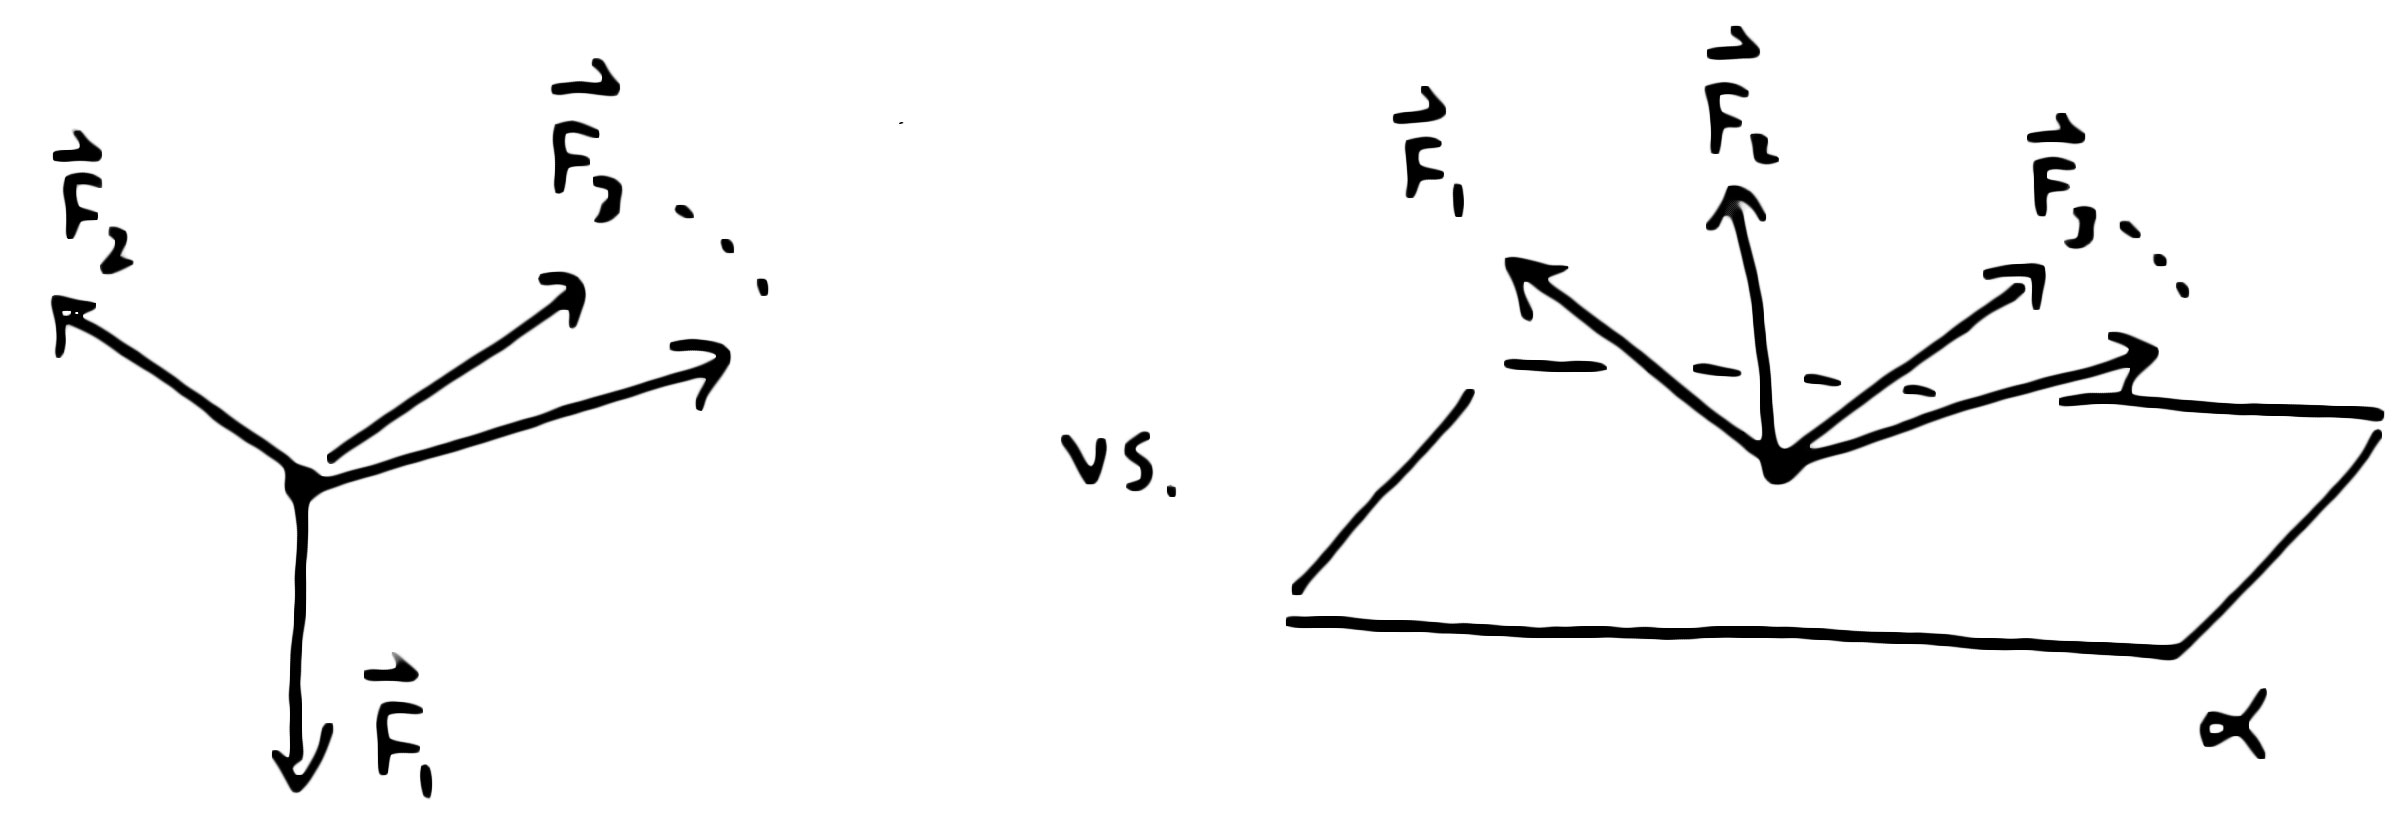
\includegraphics[width=0.85\textwidth]{vectorpossibilities.jpg}
\end{center}
\caption{On the left, a bunch of vectors that can sum to zero with positive coefficients.  On the right, a bunch of vectors that can't.  In the latter case, it's possible to find a separating plane $\a$.\label{fig:vectorpossibilities}}
\end{figure}

Equation~(\ref{eq:abstractcrossingeq}) says that a bunch of vectors sum to zero with positive coefficients.  This may or may not be possible, depending on the vectors.  The left-hand side of figure~\ref{fig:vectorpossibilities} shows a case where it's possible, and the right-hand side shows a case where it's impossible.  The way to distinguish these cases is to search for a {\it separating plane} $\alpha$ through the origin such that all the vectors $\vec{F}_{\De,\ell}^{\De_\f}$ lie on one side of $\alpha$.  If $\alpha$ exists, then the  $\vec{F}_{\De,\ell}^{\De_\f}$ cannot satisfy crossing, for any choice of coefficients $p_{\De,\ell}=f_{\f\f\cO}^2$.  This suggests the following procedure for bounding CFT data.

\begin{algorithm}[Bounding Operator Dimensions]
\label{thealgorithm}
\qquad

\begin{enumerate}
\item Make a hypothesis for which dimensions and spins $\De,\ell$ appear in the $\f\x\f$ OPE.
\item Search for a linear functional $\alpha$ that is nonnegative acting on all $\vec F_{\Delta,\ell}^{\Delta_\f}$ satisfying the hypothesis,
\be
\alpha(\vec F_{\Delta,\ell}^{\De_\f})\geq 0,
\ee
and strictly positive on at least one operator (usually taken to be the unit operator).
\item If $\alpha$ exists, the hypothesis is wrong.  We see this by applying $\alpha$ to both sides of (\ref{eq:abstractcrossingeq}) and finding a contradiction.
\end{enumerate}
\end{algorithm}

A slight modification of this algorithm also lets one bound OPE coefficients \cite{Caracciolo:2009bx}.

\subsection{An example bound}
\label{sec:boundsexample}

Let's work through an example.\footnote{An early version of this example is due to Sheer El-Showk, and this specific implementation is due to Jo\~ao Penedones and Pedro Vieira.}  Consider a 2d CFT with a real scalar primary $\f$ of dimension $\De_\f=\frac 1 8$.
Project the crossing equation onto a two-dimensional subspace with the linear map
\be
\label{eq:vecv}
\vec v(F) &= \p{H\p{\frac 1 2,\frac 3 5} - H\p{\frac 1 2, \frac 1 3}, H\p{\frac 1 2,\frac 3 5} - H\p{\frac 1 3, \frac 1 4}}\in \R^2,\nn\\
&\quad \textrm{where}\quad H(z,\bar z) = \frac{F(u,v)}{u^{\De_\f}-v^{\De_\f}},\nn\\
&\qquad \qquad \qquad\,\,\,\,\,\,\, u=z\bar z,\nn\\
&\qquad \qquad \qquad\,\,\,\,\,\,\, v= (1-z)(1-\bar z).
\ee
By linearity, the vectors $\vec v(F_{\De,\ell}^{\De_\f})$ also sum to zero with positive coefficients,
\be
\label{eq:finitedimensionalcrossing}
\sum_{\De,\ell} p_{\De,\ell} \vec v(F_{\De,\ell}^{\De_\f}) &= 0.
\ee

In figure~\ref{fig:twodvectorsexample}, we plot $\vec v(F_{\De,\ell}^{\De_\f})$ for all $\De,\ell$ satisfying the unitarity bounds (\ref{eq:unitarityboundsummary}), where the conformal blocks are given by (\ref{eq:explicitblock2d}).  We have normalized the vectors so that they are easy to see, since changes in normalization can be absorbed into the coefficients $p_{\De,\ell}$.

\begin{figure}
\begin{center}
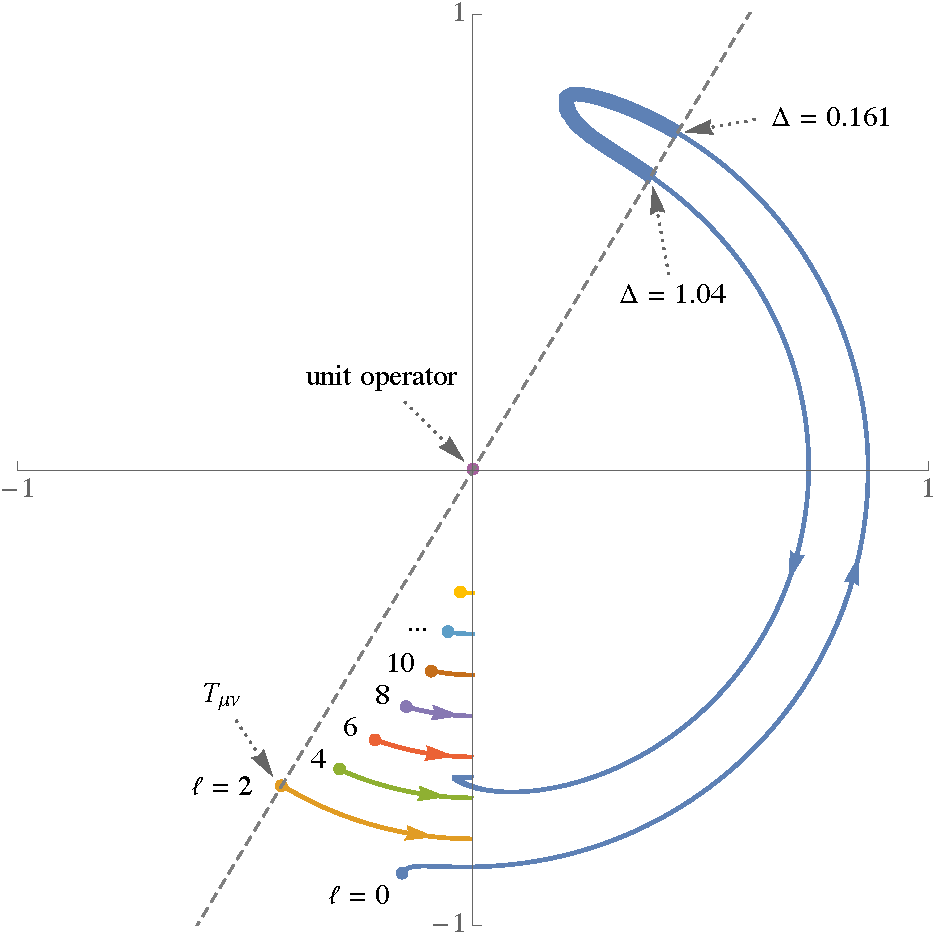
\includegraphics[width=0.9\textwidth]{2dVectorsExample}
\end{center}
\caption{Vectors $\vec v(F_{\De,\ell}^{\De_\f})$ for all values of $\De,\ell$ satisfying the 2d unitarity bound $\De\geq \ell$, with $\ell$ even.  Dots represent vectors at the unitarity bound $\De=\ell$.  As $\De$ varies, $\vec v(F_{\De,\ell}^{\De_\f})$ sweeps out a curve starting at the dot and approaching  the negative $y$-axis as $\De\to \oo$. The curves for spins $\ell=16,18,\dots$ look similar and converge quickly as $\ell\to \oo$, so we have not included them in the figure.  All vectors are normalized for visual simplicity, except for the unit operator $\vec v(F_{0,0}^{\De_\f})=\vec 0$.  The dashed line splits the figure into two half-spaces with the stress tensor $\vec v(F_{2,2}^{\De_\f})$ on the boundary.  The thicker region of the $\ell=0$ curve, in a different half-space from the rest of the figure, corresponds to scalars with dimension $\De\in[0.161,1.04]$.}
\label{fig:twodvectorsexample} 
\end{figure}

As $\De$ varies from $\ell$ (the unitarity bound) to $\oo$, $\vec v(F_{\De,\ell}^{\De_\f})$ sweeps out a curve.  The curves for higher spin operators $\ell\geq 2$ are extremely simple, converging quickly at large $\De$.  The scalar curve is more interesting. It circles counterclockwise partway around the origin before circling back and converging as $\De\to \oo$.  The region $\De\in[0.161,1.04]$ of the scalar curve lies in a different half space from the other curves.  To satisfy (\ref{eq:finitedimensionalcrossing}), we must include at least one vector from this region.  Thus, we immediately conclude
\begin{claim}
In a unitary 2d CFT with a real operator $\f$ of dimension $\De_\f=\frac 1 8$, there must exist a scalar in the $\f\x\f$ OPE with dimension $\De\in[0.161,1.04]$.
\label{claimboundone}
\end{claim}
\begin{proof}
We have already given the proof, but let us rephrase it in terms of Algorithm~\ref{thealgorithm}.
\begin{itemize}
\item Suppose (for a contradiction) that there are no scalars with $\De\in[0.161,1.04]$ in the $\f\x\f$ OPE.
\item Let
\be
\alpha(F) &= \vec u \. \vec v(F),
\ee
where $\vec v(F)$ is defined in (\ref{eq:vecv}) and $\vec u\in \R^2$ is normal to the dashed line, pointing to the bottom right in figure~\ref{fig:twodvectorsexample}.  Note that $\alpha(F_{\De,\ell}^{\De_\f})\geq 0$ for all $\De,\ell$ satisfying our hypothesis.  Further, $\alpha$ is strictly positive on at least one vector appearing in the $\f\x\f$ OPE. (To establish this, we could rotate $\vec u$ slightly so that $\alpha$ is strictly positive on the stress tensor vector. Alternatively, we could use the fact that at least one higher dimension operator must appear in the $\f\x\f$ OPE.)
\item Applying $\alpha$ to both sides of (\ref{eq:abstractcrossingeq}), we find a contradiction: $0>0$.
\end{itemize}
\end{proof}

\begin{exercise}
\label{exercise:asymptotics}
Check that $\alpha(F_{\De,\ell}^{\De_\f})\geq 0$ is true asymptotically as $\De\to \oo$ and $\ell\to \oo$.  Convince yourself that the proof of Claim~\ref{claimboundone} could be made rigorous to a mathematician's standards.
\end{exercise}

Fiddling around with two-dimensional vectors has yielded a surprisingly strong result.  The 2d Ising CFT is an example of a unitary theory with a real scalar $\s$ (the spin operator) with dimension $\De_\s=\frac 1 8$.  The lowest dimension scalar in the $\s\x\s$ OPE is the energy operator $\e$, which has $\De_\e=1$.  So our upper bound $\De_\mathrm{scalar}\leq 1.04$ is within $4$ percent of being saturated by an actual theory!

\subsection{Numerical techniques}
\label{sec:numericaltechniques}

The bound $\De_\mathrm{scalar}\in[0.161,1.04]$ is not particularly special.  If we had picked a different two-dimensional subspace (\ref{eq:vecv}), we would have gotten different numbers.  We might also consider higher-dimensional subspaces and derive even stronger results.  Although it is possible to prove bounds by hand as we did in the previous subsection, computerized searches are the current state-of-the-art.  In this section, we describe some of the techniques involved.

The hard part of Algorithm~\ref{thealgorithm} is the middle step: finding a functional $\alpha$ such that
\be
\label{eq:positivityconstraints}
\alpha(\vec F_{\De,\ell}^{\De_\f}) \geq 0,\qquad\textrm{for all $\De,\ell$ satisfying our hypothesis}.
\ee
If we want to use a computer, we have two immediate difficulties:
\begin{enumerate}
\item The space of possible $\alpha$'s is infinite-dimensional.
\item There are an infinite number of positivity constraints (\ref{eq:positivityconstraints}) --- one for each $\De,\ell$ satisfying our hypothesis.  Our hypothesis usually allows $\ell$ to range from $0$ to $\oo$, and $\De$ to vary continuously (aside from a few discrete values).\footnote{This is due to ignorance about the spectrum. Although physical CFT spectra should be discrete, we don't know exactly which discrete values $\De$ takes, and so we must include positivity constraints for continuously varying $\De$.}
\end{enumerate}

The first difficulty is easy to fix.  Instead of searching the infinite-dimensional space of all functionals, we restrict to a finite-dimensional subspace.  If we find $\alpha$ in our subspace that satisfies the positivity constraints, we can immediately rule out our hypothesis about the spectrum.  If we can't find $\alpha$, then we can't conclude anything about the spectrum: either no functional exists, or we just weren't searching a big enough subspace.

In the example from section~\ref{sec:boundsexample}, we restricted $\alpha$ to linear combinations of the components of $\vec v(F)$ in (\ref{eq:vecv}).  For numerical computations, we usually take linear combinations of derivatives around the crossing-symmetric point $z=\bar z = \frac 1 2$,
\be
\label{eq:choiceoffunctionals}
\alpha(F) &= \sum_{m+n\leq \Lambda} a_{mn}\ptl_z^m \ptl_{\bar z}^n F(z,\bar z)|_{z=\bar z=\frac 1 2},
\ee
where $\Lambda$ is some cutoff.  The functional $\alpha$ is now parameterized by a finite number of coefficients $a_{mn}$, and a computer can search over these coefficients.\footnote{Note that $F(z,\bar z)$ is symmetric under $z\leftrightarrow \bar z$ (because $u$ and $v$ are), so we can restrict $m\leq n$.  Also, $F(z,\bar z)$ is odd under $(z,\bar z)\to (1-z,1-\bar z)$, so we can restrict to $m+n$ odd. This gives $\frac 1 2\lfloor \frac{\Lambda+1}{2}\rfloor(\lfloor \frac{\Lambda+1}{2}\rfloor+1)$ coefficients.}\footnote{Sometimes these bounds appear to converge as $\Lambda$ increases, justifying post-hoc the choice of subspace (\ref{eq:choiceoffunctionals}).  However, this subspace is not always obviously the best choice.  New results might come from studying different points in the $z,\bar z$ plane, integrating against kernels $K(z,\bar z)$, or doing something more exotic.  For example, the limit $z\to 0$, with $\bar z$ fixed is known to encode interesting information about high spin operators. Finding the optimal space of functionals is an open problem.}

Getting around the second difficulty takes more care.  To solve the inequalities (\ref{eq:positivityconstraints}) on a computer, we must encode them with a finite amount of data.  It is usually sufficient to restrict $\ell\leq \ell_\mathrm{max}$ for some large cutoff $\ell_\mathrm{max}$.  After we find $\alpha$, we can go back and check afterwards that it satisfies $\alpha(F_{\De,\ell}^{\De_\f})\geq 0$ for $\ell>\ell_\mathrm{max}$, as in exercise~\ref{exercise:asymptotics}.

To deal with the continuous infinity of $\De$'s, three techniques have been used in the literature:
\begin{itemize}
\item Discretize $\De$ with a small spacing and impose a cutoff $\De_\mathrm{max}$.  We then have a finite set of linear inequalities for $a_{mn}$, which can be solved using {\it linear programming}.  This is the approach taken in the original paper on CFT bounds \cite{Rattazzi:2008pe}.

\item Use a version of the simplex algorithm (underlying many linear programming solvers) that is customized to handle continuously varying constraints, see \cite{El-Showk:2014dwa,Paulos:2014vya}.

\item Approximate the constraints (\ref{eq:positivityconstraints}) as positivity conditions on polynomials and use {\it semidefinite programming} \cite{Poland:2011ey,Kos:2013tga,Kos:2014bka,Simmons-Duffin:2015qma}.  We discuss this idea in more detail in section~\ref{app:semidefinite}.

\end{itemize}

\subsection{Improving on our hand-computed bound}

Let us compute an upper bound on the lowest-dimension scalar in the $\f\x\f$ OPE using a computer search. We will assume a $\Z_2$ symmetry under which $\f$ is odd so that $\f$ doesn't appear in its own OPE\@. The procedure is as follows
\begin{enumerate}
\item Pick a value $\De_0$ and assume that all scalars in the $\f\x\f$ OPE have dimension $\De\geq \De_0$.

\item Use a computer to search for $a_{mn}$ such that
\begin{align}
\label{eq:positivityconditioninexample}
\sum_{m+n\leq \Lambda} & a_{mn}  \ptl_z^m\ptl_{\bar z}^n F^{\De_\f}_{\De,\ell}(z,\bar z)|_{z=\bar z = \frac 1 2} \geq 0,\nn\\
\textrm{for all }\quad\ell &= 0,2,\dots,\ell_\mathrm{max},\quad\De \geq \begin{cases}
\De_0 & (\ell=0), \\
\ell+d-2 & (\ell>0).
\end{cases}
\end{align}

\item If (\ref{eq:positivityconditioninexample}) is solvable, there must exist a scalar with dimension below $\De_0$.

\end{enumerate}

The best bound is the critical value $\De_{0}^\mathrm{crit.}$ above which (\ref{eq:positivityconditioninexample}) is solvable and below which it is not. To find it, we can perform a binary search in $\De_0$, running the algorithm above at each step. By additionally varying $\De_\f$, we obtain a $\De_\f$-dependent upper bound on the lowest-dimension scalar in the $\f\x\f$ OPE.

An implementation of this procedure is included with the semidefinite program solver {\tt SDPB} \cite{Simmons-Duffin:2015qma}.\footnote{See {\tt mathematica/Bootstrap2dExample.m} at {\tt https://github.com/davidsd/sdpb}.}  See also \cite{Behan:2016dtz} for a Python interface to {\tt SDPB} and \cite{Paulos:2014vya} for another user-friendly bootstrap package.  Running the code for $\Lambda=6,8,12,16,20,28$ gives the bounds shown in figure~\ref{fig:2dbound}.\footnote{We use the {\tt SDPB} parameters listed in the appendix of \cite{Simmons-Duffin:2015qma}.}  

\begin{figure}[hrt!]
\begin{center}
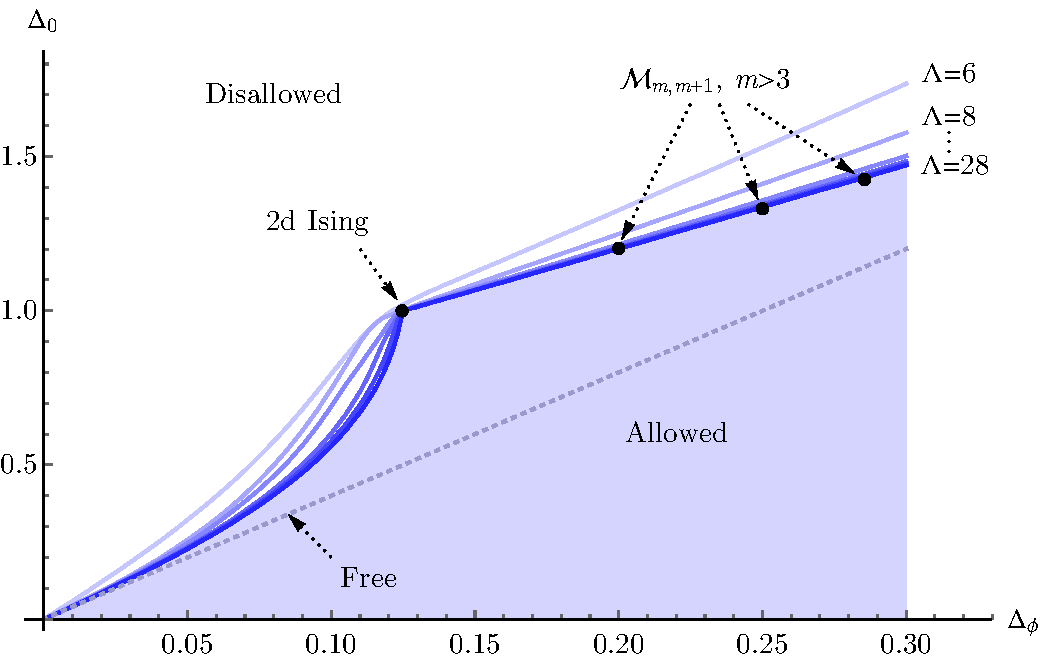
\includegraphics[width=\textwidth]{2dBound}
\end{center}
\caption{\label{fig:2dbound}
Upper bounds on the dimension $\De_0$ of the lowest dimension scalar in the $\f\x\f$ OPE as a function of $\De_\f$, for 2d CFTs with a $\Z_2$ symmetry. The bounds are computed using {\tt SDPB} for $\Lambda=6,8,12,16,20,28$, with the strongest bound (darkest blue curve) corresponding to $\Lambda=28$ (a 105-dimensional space of functionals). The black dots represent the unitary minimal models $\mathcal{M}_{m,m+1}$ with $(\De_\f,\De_0)=(\frac 1 2 - \frac{3}{2(m+1)},2-\frac{4}{m+1})$ for $m=3,4,5,6$, of which the 2d Ising model is the case $m=3$.  The dashed line represents the lowest dimension scalar in an OPE of operators $\cos(k\phi)$ in the free boson theory.  These bounds first appeared in~\cite{Rychkov:2009ij}. It should be possible to improve on the lower bound in section~\ref{sec:boundsexample} as well, though we have not attempted this.
}
\end{figure}

As the cutoff $\Lambda$ on the number of derivatives increases, the bounds $\De_0^\mathrm{crit.}(\De_\f)$ get stronger. Remarkably, the strongest bounds are nearly saturated by interesting physical theories. The most obvious feature of figure~\ref{fig:2dbound} is a {\it kink\/} near the location of the 2d Ising model $(\De_\f,\De_0)=(\frac 1 8,1)$.  (Other exactly soluble unitary minimal models $\mathcal{M}_{m,m+1}$ also lie near the bound.) The bounds for different $\Lambda$ at the 2d Ising point $\De_\f=\frac 1 8$ are given in table~\ref{tab:twodbounds}.  Taking $\Lambda=28$ gives a bound $\De_\e \leq \De_0^\mathrm{crit.}(\frac 1 8)\approx 1.0000005$, within $5\x 10^{-7}$ of the correct value.

\begin{table}[ht]
\tbl{\label{tab:twodbounds} Upper bounds on $\De_\e$ in the 2d Ising model, computed with different cutoffs $\Lambda$ on the number of derivatives.}{
\begin{tabular}{c|c|c|c|c|c|c}
$\Lambda$  & 6 & 8 & 12 & 16 & 20 & 28 \\
\hline
$\De_0^\mathrm{crit.}(\De_\f=\frac 1 8)$ & 1.020 & 1.0027 & 1.00053 & 1.000043 & 1.0000070 & $\sim1.0000005$
\end{tabular}}
\end{table}

\subsection{Numerical results in 3d}

It is helpful to compare to exact solutions in 2d, but the above results are remarkable because the methods are so general. We input information about 2d global conformal symmetry (nothing about the Virasoro algebra!) and unitarity, and the 2d Ising model pops out.  Wonderfully, the same thing happens in 3d! Again, we compute an upper bound on the lowest dimension scalar in the $\f\x\f$ OPE, this time using the 3d conformal blocks and the 3d unitarity bound.  The resulting bound, shown in figure~\ref{fig:singletbound3d}, has a kink at $(\De_\f,\De_0)\approx(0.518,1.412)$ --- close to the values realized in the 3d Ising CFT \cite{ElShowk:2012ht}.

\begin{figure}[hrt!]
\begin{center}
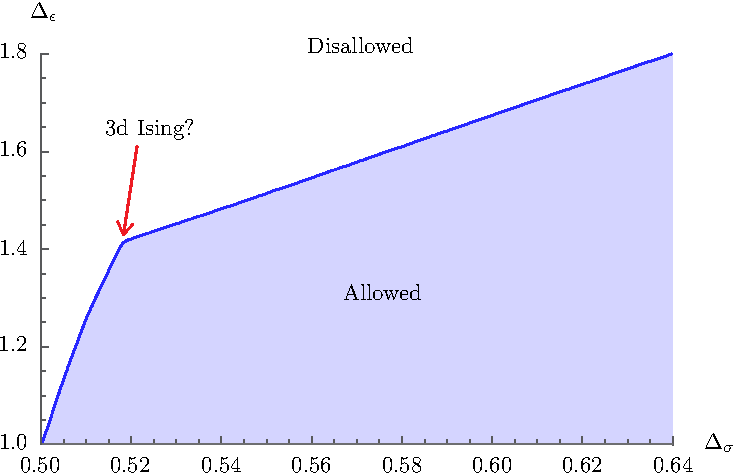
\includegraphics[width=\textwidth]{singleCorrelator3dBound}
\end{center}
\caption{\label{fig:singletbound3d} Upper bound on the dimension $\De_\e$ of the lowest dimension scalar in the $\s\x\s$ OPE, where $\s$ is a real scalar primary in a unitary 3d CFT with a $\Z_2$ symmetry, from \cite{El-Showk:2014dwa}. This bound is computed with $\Lambda=24$ (78-dimensional space of derivatives).}
\end{figure}

All the results discussed so far come from studying crossing symmetry of a single four-point function.  However, the techniques can be generalized to systems of correlation functions. The system $\<\s\s\s\s\>$, $\<\s\s\e\e\>$, $\<\e\e\e\e\>$ in the 3d Ising CFT was studied in \cite{Kos:2014bka}.  To get interesting new bounds in this case, it's necessary to input an additional fact: that $\s$ and $\e$ are the only relevant scalars in the theory.\footnote{This is an obvious experimental fact about the 3d Ising CFT. (It would be interesting to prove mathematically.)  Relevant scalars are in one-to-one correspondence with parameters that must be tuned to reach the critical point in some microscopic theory.  The fact that the phase diagram of water is 2-dimensional (the axes are temperature and pressure) tells us that the critical point of water has two relevant operators.}  In practice, this roughly means that we impose positivity conditions $\alpha(F_{\De,\ell})\geq 0$ for $\De=\De_\s,\De_\e$, and $\De\geq 3$.  The resulting bound in figure~\ref{fig:multicorrelator3d} now restricts $(\De_\s,\De_\e)$ to a small island in the space of operator dimensions.

\begin{figure}[hrt!]
\begin{center}
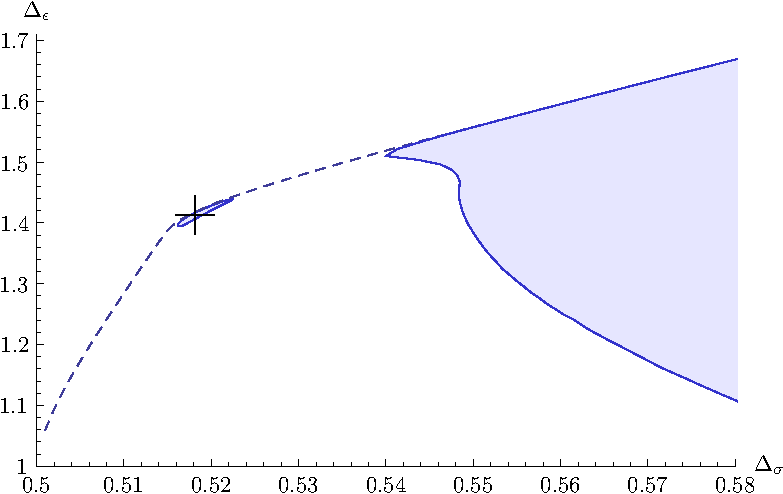
\includegraphics[width=\textwidth]{multiCorrelator3dBound}
\end{center}
\caption{\label{fig:multicorrelator3d} Bound on $(\De_\s,\De_\e)$ in a unitary 3d CFT with a $\Z_2$ symmetry and two relevant scalars $\s,\e$ with $\Z_2$ charges $-,+$.  The bound comes from studying crossing symmetry of $\<\s\s\s\s\>$, $\<\s\s\e\e\>$, $\<\e\e\e\e\>$, and is computed with $\Lambda=12$.  The allowed region is now a small island near the 3d Ising point (black cross), with an additional bulk region to the right.}
\end{figure}

The same multiple correlator bound, computed with $\Lambda=43$ using {\tt SDPB}, is shown in figure~\ref{fig:sdpbBound} \cite{Simmons-Duffin:2015qma}.  The island has shrunk substantially, giving a precise determination of the 3d Ising operator dimensions,
\be
(\De_\s,\De_\e) &= (0.518151(6), 1.41264(6)).
\ee
Figures~\ref{fig:multicorrelator3d} and~\ref{fig:sdpbBound} are conceptually interesting.  Firstly, the striking agreement between Monte Carlo simulations and the conformal bootstrap is strong evidence that the critical 3d Ising model actually does flow to a conformal fixed-point, as originally conjectured by Polyakov \cite{Polyakov:1970xd}.

Secondly, figures~\ref{fig:multicorrelator3d} and~\ref{fig:sdpbBound} give a way to understand the phenomenon of critical universality discussed at the beginning of this course.  If a theory flows to a unitary 3d CFT with a $\Z_2$-symmetry and two relevant scalars $\s,\e$ --- and if $\De_\s,\De_\e$ don't live in the bulk region in figure~\ref{fig:multicorrelator3d} --- then the IR theory must live in the 3d Ising island!  Perhaps future bootstrap studies will shrink the 3d Ising island to a point, proving the IR equivalence of these theories.

\begin{figure}[hrt!]
\begin{center}
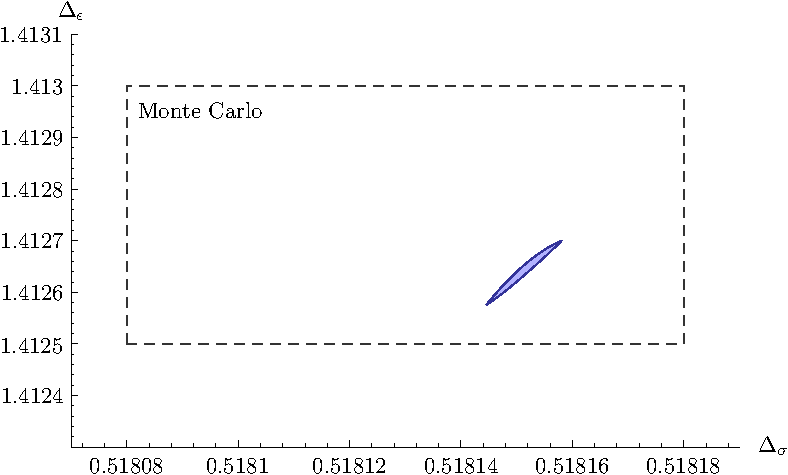
\includegraphics[width=\textwidth]{sdpbBound}
\end{center}
\caption{\label{fig:sdpbBound} Bound on $(\De_\s,\De_\e)$ in a unitary 3d CFT with a $\Z_2$ symmetry and two relevant scalars $\s,\e$ with $\Z_2$ charges $-,+$.  The bound comes from studying crossing symmetry of $\<\s\s\s\s\>$, $\<\s\s\e\e\>$, $\<\e\e\e\e\>$, and is computed with $\Lambda=43$ using {\tt SDPB}. The allowed region is the blue sliver. The dashed rectangle shows the $68\%$ confidence region for the current best Monte Carlo determinations.}
\end{figure}


%\section*{Acknowledgements}
%
%I am grateful to Joe Polchinski and Pedro Vieira for inviting me to give this course, and Tom DeGrand, Oliver DeWolfe, and Sherry Namburi for helping make TASI such a fun experience.  I am also grateful to Justin David, Chethan Krishnan and Gautam Mandal for organizing the Advanced Strings School at ICTS, Bangalore.  A special thanks to the spectacular students at TASI and the Strings School, who asked so many good questions.  Thanks to Chris Beem, Joanna Huey, Filip Kos, Petr Kravchuk, David Poland, and Slava Rychkov for comments.  Thanks to Sheer El-Showk, Jo\~ao Penedones, and Pedro Vieira for the nice example in section~\ref{sec:boundsexample}. I am supported by DOE grant number DE-SC0009988 and a William D. Loughlin Membership at the Institute for Advanced Study.


%\begin{appendix}[Quantization of the Lattice Ising Model]
%\label{app:latticequantization}
%
%In this section, we show how to interpret the partition function of the Ising model on a square lattice in terms of Hilbert spaces and discrete time evolution.  This is a textbook trick,\footnote{It is the starting point for Onsager's exact solution of the 2d Ising model \cite{PhysRev.65.117}.} but we review it because it clearly illustrates several ideas from section~\ref{sec:quantization}.
%
%Consider the 2d Ising model on an $m\x n$ lattice with periodic boundary conditions.  The spins are given by $s_{i,j}\in \{\pm 1\}$, where $i\in \Z/m\Z$ and $j\in \Z/n\Z$.  The partition function is
%\be
%\label{eq:isingpartitionfunction}
%Z &= \sum_{\{s\}} \exp\p{-JS_h(s) -J S_v(s)},\nn\\
%S_h(s) &\equiv& \sum_{i,j} s_{i,j}s_{i+1,j},\nn\\
%S_v(s) &\equiv& \sum_{i,j} s_{i,j} s_{i,j+1},
%\ee
%where we have separated the action into contributions from horizontal and vertical bonds.
%
%We will think of the $j$-direction as ``time", and introduce a Hilbert space $\cH_m$ associated with a ``slice" of $m$ lattice sites at constant time.  The space $\cH_m$ has a basis state for each spin configuration on the slice,
%\be
%|s_1,\dots,s_m\>,\qquad s_i\in\{\pm 1\}.
%\ee
%These are the analogs of the field eigenstates $|\phi_b\>$ in section~\ref{sec:operatorimpliesstate}.
%The Pauli spin matrices $\widehat\sigma_i^{\mu}$, $\mu=x,y,z$ act on the $i$-th site.
%
%The operator
%\be
% U &\equiv & \exp\p{-J\sum_{i=1}^m \widehat\s^z_i \widehat\s^z_{i+1}}
%\ee
%encodes the contribution to the partition function from horizontal bonds between $m$ spins in a line. For example on an $m\x 1$ lattice, we would have
%\be
% U |s_1,\dots,s_m\> &= e^{-JS_h(s)}|s_1,\dots,s_m\>.
%\ee
%The operator
%\be
% V &\equiv& \prod_i(e^{-J} + e^{J}\widehat\s_i^x)
%\ee
%encodes the effects of vertical bonds. For each site, it either preserves the spin, giving a factor $e^{-J}$ associated with aligned spins, or flips it, giving a factor $e^{J}$ associated with anti-aligned spins.  Defining the ``transfer matrix" $ T\equiv VU$, it's easy to check that
%\be
%Z &= \Tr_{\cH_m}( T^n).
%\ee
%
%We have interpreted the discrete path integral (\ref{eq:isingpartitionfunction}) in terms of operators on a Hilbert space.  The transfer matrix is a discrete analogue of the time-evolution operator $e^{-tH}$.  The path integral variable $s_{i,j}$ maps to the quantum operator
%\be 
%\label{eq:quantizationmapone}
%s_{i,j} &\to& T^{-j} \s_i^z  T^j,
%\ee
%and correlation functions become traces of time-ordered products, e.g.\footnote{We use the convention $\th(0)=\frac 1 2$.}
%\be
%\<\s_{i_1,j_1}\s_{i_2,j_2}\> &= \Tr_{\cH_m}(T^{n+j_2-j_1} \widehat \s_{i_1}^z T^{j_1-j_2} \widehat \s_{i_2}^z)\theta(j_1 - j_2) + (1\leftrightarrow 2).\nn\\
%\ee
%
%We could instead have quantized the theory with the horizontal direction as time.  This would give a different Hilbert space $\cH_n$ with dimension $2^n$ instead of $2^m$, a new transfer matrix $T'$ (acting on $\cH_n$), and a different formula for the same path integral
%\be
%Z &= \Tr_{\cH_n}(T'^m)=\Tr_{\cH_m}(T^n).
%\ee
%The new quantization map would be
%\be
%\label{eq:quantizationmaptwo}
%s_{i,j} &\to& T'^{-i} \widehat \s_j^z T'^i.
%\ee
%Let us emphasize that the operators (\ref{eq:quantizationmapone}) and (\ref{eq:quantizationmaptwo}) are truly different, even though they represent the same path integral variable.  They even act on different-dimensional Hilbert spaces ($2^m$ vs.\ $2^n$)!  Thus, it's not surprising that properties associated to a particular quantization, like their behavior under Hermitian conjugation (section~\ref{sec:reflectionpositivity}), could be different.
%
%\vspace{0.2in}
%
%\end{appendix}
%
%\begin{appendix}[Euclidean vs. Lorentzian and Analytic Continuation]
%\label{app:analyticcontinuation}
%
%Here we make some brief comments about Euclidean and Lorentzian correlation functions and analytic continuation between them.  
%
%The first comment is that in Euclidean quantum field theory, out-of-time-order correlators don't make sense.  For example, consider a Euclidean two-point function,
%\be
%\label{eq:euclideantwopt}
%\<0|\cO_1(t_1)\cO_2(t_2)|0\> &= \<0| \cO_1(0) e^{H(t_2-t_1)} \cO_2(0)|0\>.
%\ee
%In QFT, the Hamiltonian $H$ is bounded from below and has arbitrarily large positive eigenvalues.  If we take $t_2 > t_1$, then the operator $e^{H(t_2-t_1)}$ is unbounded.  Generically, local operators $\cO_{1,2}(0)$ have nonzero amplitude to create arbitrarily high energy states. Thus, (\ref{eq:euclideantwopt}) is formally infinite.
%
%Because the Euclidean path integral gives a time-ordered product
%\be
%\label{eq:euclideantimeorderedproduct}
%\<\cO_1(t_1)\cO_2(t_2)\> &= \<0|\cO_1(0)e^{H(t_2-t_1)}\cO_2(0)|0\>\th(t_1-t_2)+\nn\\
%& \<0|\cO_2(0)e^{H(t_1-t_2)}\cO_1(0)|0\>\th(t_2-t_1),
%\ee
%it is well-defined for any ordering of the time coordinates. Specifically, the operators $e^{H(t_i-t_j)}$ in (\ref{eq:euclideantimeorderedproduct}) are always bounded.
%
%In Lorentzian quantum field theory, however,  non-time-ordered correlators (Wightman functions) are interesting observables.  They can be obtained from time-ordered Euclidean correlators as follows.  First set the Euclidean times equal to small values $t_{Ei}=\e_i$, increasing in the same order as the operator ordering we want.  For example, to place $\cO_1$ later than $\cO_2$, consider
%\be
%\<\cO_1(\e)\cO_2(0)\> &= \<0|\cO_1(0)e^{-\e H}\cO_2(0)|0\>,\qquad \e>0.
%\ee
%Now continue $t_{Ei}$ in the pure imaginary direction to the desired Lorentzian times $it_{Li}$.  Because $e^{H(t_{Ei}-t_{Ej})}$ never becomes unbounded, the operators remain in the same order,
%\be
%\<\cO_1(\e+i t_{L1})\cO_2(it_{L2})\> &= \<0|\cO_1(0)e^{-\e H - iH(t_{L1}-t_{L2})}\cO_2(0)|0\>.
%\ee
%Finally, take $\e\to 0$ to get the desired Wightman function.
%
%To get a time-ordered Lorentzian correlator, there is a simple trick: just simultaneously rotate all Euclidean times $t\to i (1-i\e) t$. Because the ordering of the real parts of $t$ are preserved, the order of the operators will be too. This is Wick rotation.
%
%Many properties of correlators under analytic continuation are clearer when thinking about states and Hamiltonians, as opposed to path integrals.
%
%\vspace{0.2in}
%
%\end{appendix}

\subsection{Semidefinite programming}
\label{app:semidefinite}

For our purposes, a semidefinite program solver is an oracle that can solve the following problem:
\be
\label{eq:semidefiniteprogram}
\textrm{Find $\vec a$ such that $\vec a \. \vec P_i(x) \geq 0$ for all $x\geq 0$, $i=1,\dots,N$},
\ee
where $\vec P_i(x)$ are vector-valued polynomials.  There are many freely-available semidefinite program solvers.  {\tt SDPB} \cite{Simmons-Duffin:2015qma} in particular was written for application to the conformal bootstrap.

We would like to write our search in the form (\ref{eq:semidefiniteprogram}).
After restricting to the subspace (\ref{eq:choiceoffunctionals}), our positivity constraints become
\be
\label{eq:positivityinfinitespace}
\sum_{m+n\leq \Lambda} a_{mn}\ptl_z^m \ptl_{\bar z}^n F_{\De,\ell}^{\De_\f}(z,\bar z)|_{z=\bar z = \frac 1 2} \geq 0.
\ee
The trick is to find an approximation
\be
\label{eq:polynomialapproximation}
\ptl_z^m \ptl_{\bar z}^n F_{\De,\ell}^{\De_\f}(z,\bar z)|_{z=\bar z= \frac 1 2} &\approx \chi_\ell(\De) P^{mn}_\ell(\De),
\ee
where $\chi_\ell(\De) \geq 0$ are positive and $P^{mn}_\ell(\De)$ are polynomials.  Then, dividing (\ref{eq:positivityinfinitespace}) by $\chi_\ell(\De)$ and writing $\De=\De_{\mathrm{min},\ell}+x$, our inequality becomes
\be
\sum_{m+n\leq \Lambda} a_{mn} P_\ell^{mn}(\De_{\mathrm{min},\ell}+x) &\geq 0.
\ee
This has the right form if we group the coefficients $a_{mn}$ into a vector $\vec a$ and identify $\ell\to i$, $\ell_\mathrm{max}\to N$.  The value $\De_{\mathrm{min},\ell}$ depends on the calculation at hand, see for example (\ref{eq:positivityconditioninexample}).

To get a positive-times-polynomial approximation, we can start with the series expansion (\ref{eq:seriesexpansion}),
\be
g_{\De,\ell}(u,v) &= \sum_{n,j} B_{n,j} r^{\De+n} C_j^{\frac{d-2}{2}}(\cos\th).
\ee
Recall that the coefficients $B_{n,j}$ are positive rational functions of $\De$.  The crossing-symmetric point $z=\bar z = \frac 1 2$ corresponds to a very small value of $r=r_*=3-2\sqrt 2 \approx 0.17$.  Thus, truncating the series at some large $n_\mathrm{max}$ gives a good approximation,
\be
\ptl_r^a \ptl_\th^b g_{\De,\ell}(u,v)|_{r=r_*,\th=0} &\approx r_*^\De \frac{P^{ab}_\ell(\De)}{Q_\ell(\De)}  + O(r_*^{\De+n_\mathrm{max}}),
\ee
where $P^{ab}_\ell$ and $Q_\ell$ are polynomials and $Q_\ell(\De)$ is positive.  Since derivatives of $F_{\De,\ell}^{\De_\f}(z,\bar z)$ are linear combinations of derivatives of $g_{\De,\ell}(u,v)$, this establishes (\ref{eq:polynomialapproximation}) with
\be
\chi_\ell(\De) &= \frac{r_*^\De}{Q_\ell(\De)}.
\ee

When exact formulae for conformal blocks are not available (for example, in odd dimensions), the polynomials $P^{ab}_\ell(\De)$ can be computed using recursion relations \cite{Zamolodchikov:1985ie,Zamolodchikov:1987,Kos:2013tga,Kos:2014bka,Penedones:2015aga,Yamazaki:2016vqi,Iliesiu:2015akf} or differential equations \cite{Hogervorst:2013kva}.

\subsection{Open questions}

The techniques above have been applied to numerous theories in different spacetime dimensions, with different amounts of supersymmetry \cite{Rattazzi:2008pe, Rychkov:2009ij, Caracciolo:2009bx, Poland:2010wg, Rattazzi:2010gj, Rattazzi:2010yc, Vichi:2011ux, Poland:2011ey, Rychkov:2011et, ElShowk:2012ht,Liendo:2012hy, Beem:2013qxa, Kos:2013tga, El-Showk:2013nia, Alday:2013opa, Gaiotto:2013nva,Bashkirov:2013vya, Berkooz:2014yda, El-Showk:2014dwa, Nakayama:2014lva,Nakayama:2014yia, Alday:2014qfa, Chester:2014fya, Kos:2014bka, Caracciolo:2014cxa, Nakayama:2014sba, Golden:2014oqa, Chester:2014mea, Paulos:2014vya, Beem:2014zpa, Simmons-Duffin:2015qma, Bobev:2015vsa, Bobev:2015jxa, Kos:2015mba, Chester:2015qca, Beem:2015aoa, Iliesiu:2015qra,poland2015exploring,Lemos:2015awa,Lin:2015wcg,Chester:2015lej,Chester:2016wrc}.  Because we don't start with a Lagrangian, there's no guarantee when and how a particular physical theory will show up in the bounds. It's an open question which correlators to study to isolate different CFTs.

Other open questions include the following:
\begin{itemize}
\item How do the bounds behave in the limit $\Lambda\to \oo$? Does the Ising island shrink to a point, still using a finite number of correlation functions, or must we study larger systems of crossing equations?
\item How does one efficiently compute higher operator dimensions and OPE coefficients?  The extremal functional method \cite{Poland:2010wg,ElShowk:2012hu,El-Showk:2014dwa} is one way, but it is hard to estimate the associated errors.
\item Can the requirement of unitarity be relaxed? Gliozzi's method of determinants \cite{Gliozzi:2013ysa} has shown success analyzing the crossing equation in nonunitary theories and other situations where positivity is not obviously present \cite{Gliozzi:2014jsa,Gliozzi:2015qsa,Nakayama:2016cim}. Can it be made rigorous?
\item What information is hidden in correlators of higher-spin operators like stress tensors?
\item What can we prove analytically about the crossing equations? Progress has been made in certain limits, for example large-$N$ \cite{Heemskerk:2009pn}, large dimension \cite{Pappadopulo:2012jk}, large spin \cite{Alday:2007mf,Fitzpatrick:2012yx,Komargodski:2012ek,Alday:2015ewa}, and combinations thereof \cite{Fitzpatrick:2014vua,Fitzpatrick:2015qma,Fitzpatrick:2015zha}. Another approach is to study the implications of slightly broken symmetries \cite{Maldacena:2012sf,Rychkov:2015naa,Alday:2015ota,Skvortsov:2015pea,Giombi:2016hkj}. It would be extremely interesting to prove analytical results about the small-$N$, small $\De,\ell$ regime.
\item What additional structures and consistency conditions should we incorporate into the bootstrap? (See section~\ref{sec:additionalstructures}.)
\item What protected information can be computed using supersymmetry? Bootstrap studies recently led to the discovery of beautiful new algebraic structures in the OPE algebra of supersymmetric theories in $3,4,6$ dimensions \cite{Beem:2013sza,Chester:2014mea,Beem:2016cbd}. How do these structures interact with the full non-protected bootstrap? 
\end{itemize}

That's a lot of open questions, and there are certainly many more.
I hope some of you will help find the answers!


\bibliographystyle{ws-rv-van}
\bibliography{ph229-notes}
\ifarxivsubmission
\else
  \blankpage
\fi
\printindex
\end{document}
